\documentclass[a4paper,8pt,titlepage]{scrbook}

\usepackage[T1]{fontenc}
\usepackage[utf8]{inputenc}
\usepackage[ngerman]{babel}
\usepackage{hyperref}
\usepackage{tabularx}
\usepackage{amsmath}
\usepackage{amssymb}
\usepackage{graphicx}
\usepackage{listings}
\usepackage{listings_glsl}
\usepackage{listings_mips}
\usepackage{listings_vhdl}
\usepackage[ruled,vlined]{algorithm2e}
\usepackage{esdiff}
\usepackage{float}
\usepackage{placeins}
\usepackage{lscape}
\usepackage{array}
\usepackage{geometry}
\geometry{left=2cm,right=2cm,top=2cm,bottom=2cm,bindingoffset=10mm}
\restylefloat{table}

\usepackage{enumitem}
\setlistdepth{20}
\renewlist{itemize}{itemize}{20}
\setlist[itemize]{label=$\cdot$}
\setlist[itemize,1]{label=\textbullet}
\setlist[itemize,2]{label=--}
\setlist[itemize,3]{label=\(\ast\)}

\usepackage{subcaption}
\usepackage{tikz}
\usetikzlibrary{calc}
\usetikzlibrary{decorations.pathreplacing}
\usetikzlibrary{shapes}

\title{Vorlesungen am Karlsruher Institut für Technologie}
\author{Maximilian Heß}
\date{September 2017}

\begin{document}
\maketitle
\tableofcontents

\part{Bachelor}
\include{algo2}
\include{algo2algorithmen}
\include{bwlc}
\include{computergrafik}
\include{echtzeitsysteme}
\include{financial_management}
\include{investments}
\include{it_sicherheitsmanagement}
\chapter{Programmierparadigmen}

Zusammenfassung der Vorlesung "`Programmierparadigmen"' aus dem Wintersemester 2014.\footnote{\url{https://pp.info.uni-karlsruhe.de/lehre/WS201415/paradigmen/}}

\section{Funktionale Programmierung (S16)}

\subsection{Einführung: Funktionale Programmierung in Haskell}
\begin{itemize}
	\item Funktionale Programme sind kompakt, frei von Seiteneffekten, unabhängig von der Anweisungsreihenfolge
	\item Der Begriff \textit{Funktion} in Sprachen wie Haskell entspricht der mathematischen Sicht: Ausgaben hängen lediglich von Eingaben ab \(\rightarrow\) Auswertungen haben keinen Effekt auf Daten des Programms.
	\item Haskellprogramme sind Folgen von Funktionsdefinitionen
\end{itemize}

\subsection{Rekursion (S27)}
\begin{itemize}
	\item Auswertung: Zwischenausdrücke können mit Eingabegröße wachsen
	\item Speicherverbrauch in \(\mathcal{O}(n)\) bei \(\mathcal{O}(n)\) Aufrufen
	\item \textbf{Akkumulation}
	\begin{itemize}
		\item Übergebe Zwischenergebnisse in Hilfsparameter \texttt{acc}
		\item Speicherverbrauch in \(\mathcal{O}(1)\) bei \(\mathcal{O}(n)\) Aufrufen
	\end{itemize}
\end{itemize}

\subsubsection{Endrekursion (S30)}
\begin{itemize}
	\item Linearität: Eine Funktion heißt \textit{linear rekursiv}, wenn in jedem Defitionszweig nur ein rekursiver Aufruf vorkommt.
	\item Endrekursion: Eine linear rekursive Funktion heißt \textit{endrekursiv}, wenn in jedem Zweig der rekursive Aufruf nicht in andere Aufrufe eingebettet ist.
\end{itemize}


\subsection{Listen (S34)}
\begin{itemize}
	\item Eine Liste \texttt{(x:xs)} besteht immer aus Listenkopf \texttt{x} und Listenrest \texttt{xs}
\end{itemize}

\subsubsection{Pattern Matching (S37)}
\begin{itemize}
	\item Mehrere Gleichungen zur Definition einer Funktion
	\item Jede Gleichung gilt für Argumente mit speziellem Strukturmuster
	\item Überlappende Muster: Erste Gleichung wird angewandt
\end{itemize}


\subsection{Funktionen höherer Ordnung (S44)}

\subsubsection{Lambda-Notation (S45)}
\begin{itemize}
	\item Anonyme Funktionen und Funktionen höherer Ordnung möglich
	\item Beispiel: \(g(x,y)=x-\frac{y}{2} \longrightarrow\) \texttt{g = \textbackslash x y -> x - 2/y}
\end{itemize}

\subsubsection{Definition: Funktion höherer Ordnung (S47)}
Funktionen, die andere Funktionen als Parameter erhalten oder Funktionen als Rückgabewerte liefern, heißen Funktionen höherer Ordnung.

\subsubsection{Currying (S50)}
\begin{itemize}
	\item Ersetzung einer mehrstelligen Funktion durch Schachtelung einstelliger Funktionen.
	\item Jede Funktion erhält, wie oben erwähnt, nur ein Argument. Werden scheinbar mehrere Argumente definiert, so steckt immer Currying dahinter.
	\item Unterversorgung: Anwendung mehrstelliger Funktionen auf zu wenig Parameter
\end{itemize}

\textbf{Beispiel\footnote{\url{https://de.wikipedia.org/wiki/Currying\#Haskell}}}

\begin{lstlisting}[frame=single,numbers=left,mathescape,language=Haskell]
addiere x y = x + y
addiere 1 3                -- ist aequivalent zu (addiere 1) 3
addiereZu2  = addiere 2
addiereZu2 1               -- 3
\end{lstlisting}

\subsubsection{Namensbindung (S54)}
\begin{itemize}
	\item Bindungsstrukte legen Bedeutung und Geltungsbereiche von Variablen fest
	\item Verdeckung: Innere Bindungen verdecken äußere
	\item \textbf{Bindung}
	\begin{itemize}
		\item \texttt{f x = x*x}: Bindung von \texttt{x} im Rumpf von \texttt{f}, globale Bindung von \texttt{f}
		\item \texttt{\textbackslash x -> x*x}: Bindung von \texttt{x} innerhalb des \(\lambda\)-Ausdrucks
	\end{itemize}
\end{itemize}

\subsubsection{Lokale Bindung (S57)}
\begin{itemize}
	\item Anwendung: Lokale Hilfsfunktionen
	\item \texttt{let} bindet stärker als \texttt{where}
\end{itemize}

\textbf{Beispiele}

\begin{lstlisting}[frame=single,numbers=left,mathescape,language=Haskell]
energy m = let c = 299792458
           in m * c * c

energy m = m * c * c
  where c = 299792458
\end{lstlisting}

\subsection{Kombinatoren (S64)}

\subsubsection{Folds (S65)}
\begin{itemize}
	\item Anwendung einer Operation und eines Initialwertes auf eine Liste
	\item \textbf{Beispiel Summenberechnung}
	\begin{itemize}
		\item \texttt{sum = (+) 0}
		\item Berechnung mittels \texttt{foldr}: \texttt{(1 + (2 + (3 + (4 + 0))))} (rechts-geklammert)
		\item Berechnung mittels \texttt{foldl}: \texttt{((((1 + 0) + 2) + 3) + 4)} (links-geklammert)
	\end{itemize}
	\item Anwendung: Koplexe Funktionen als Kombination einfacher Funktionen
\end{itemize}

\subsubsection{Kombination von Listen (S67)}
\begin{itemize}
	\item Zusammenfügen von Listen per Reißverschluss: \texttt{zip = zipWith (,)}
	\item \texttt{zipWith} definiert eine Zusätzliche Operation
	\item Bricht ab, wenn eine der Listen keine weiteren Elemente enthält
\end{itemize}

\subsubsection{List Comprehensions (S67)}
\begin{itemize}
	\item Automatisiertes Erzeugen von Listen, basierend auf bereits existierenden Listen
	\item Inspiriert durch die mathematische Mengenschreibweise: \texttt{s = {[} 2 * x {|} x <- {[}0..{]}, x\textasciicircum 2 > 3 {]} } \footnote{\url{https://en.wikipedia.org/wiki/List_comprehension\#Haskell}}
	\item Multidimensionale Liste: \texttt{s = {[} 2*x*y {|} x <- {[}0..{]}, x\textasciicircum2 > 3, y <- {[}1,3..x{]}, y\textasciicircum2 < 100-x\textasciicircum2 {]}}
	\item Bei mehrdimensionaler Eingabe: Nur die erste Liste gegen Unendlich laufen lassen (siehe Klausur WS1314, Aufgabe 1)
\end{itemize}


\subsection{Lazy Evaluation (S70)}

\subsubsection{Auswertung (S73)}
\begin{itemize}
	\item Struturierte Daten: Nur auswerten, falls wirklich benötigt wird
	\item Duplizierte Argumente: Auswertung maximal einmal (\textit{sharing})
	\item Pattern-Matching: So weit wie nötig, bis passendes Muster gematched
	\item Boolsche Operatoren: Auswertung bis zum ersten \textit{false} (\textit{short-circuit-Auswertung})
	\item \textbf{Nachteile}
	\begin{itemize}
		\item Erschwerte Fehlersuche
		\item Fehler, die beim Testen nicht beachten wurden, tauchen eventuell später im Betrieb auf
	\end{itemize}
\end{itemize}


\subsection{Typen (S82)}
\begin{itemize}
	\item Haskell ist statisch typisiert
	\item Jeder gültige Ausdruck hat immer einen Typ und wertet immer zu gültigen Werten dieses Typs aus
	\item Schreibweise: \texttt{e :: t} falls Ausdruck \texttt{e} und Typ \texttt{t}
	\item Untypisierbare Ausdrücke erzeugen Übersetzerfehler
	\item Haskell erkennt den korrekten Typ (fast immer) zuverlässig, optional manuelle Deklaration möglich
\end{itemize}

\subsubsection{Polymorphe Typen (S86)}
\begin{itemize}
	\item Der Listen-Typ sind polymorph, die Typvariable \texttt{{[}t{]}} steht auch für Nicht-Basistypen
	\item Typvariablen parametrisieren polymorphe Typen
	\item Typkonstruktoren wie \texttt{{[} {]}} erzeugen neue Typen aus bestehenden
	\item \textbf{Funktionstypen}
	\item Funktionstypen sind ebenfalls polymorph
\end{itemize}

\subsubsection{Beispiele}
\begin{itemize}
	\item Typen mehrstelliger Funktionen: \texttt{f x y = x * y, f :: Integer -> Integer -> Integer}
	\item Typen eingebauter Operatoren: \texttt{(<=) :: Integer -> Integer -> Bool}
	\item Tupel: \texttt{(3, True) :: (Integer, Bool); (not, 7) :: (Bool -> Bool, Integer)}
\end{itemize}

\subsubsection{Typinferenz (S91)}
Errechnen der Typen durch den Compiler, dadurch entstehen kompakte Programme, die trotzdem typsicher sind. Manuelle Deklaration ist dennoch möglich.

\subsubsection{Typsynonyme (S93)}
Ableiten neuer Typen aus vorhandenen. Z.B. \texttt{type String = {[}char{]}} (kann die Lesbarkeit erhöhen). Es werden keine explizit neuen Typen erzeugt.

\subsubsection{Typen bei der Fehlersuche (S94)}
\begin{itemize}
	\item Typendeklarationen können beim Lokalisieren von Programmfehlern helfen
	\item Beabsichtigten Typ der Funktion deklarieren
	\item \textbf{Beispiel}
	\begin{itemize}
		\item \texttt{isDigit :: Char -> Bool}\\\texttt{isDigit c = isIn c "0123456789"}
		\item \texttt{*Main> isDigit '3'} würde zu einem Typfehler führen
	\end{itemize}
\end{itemize}

\subsubsection{Mengen (S95)}
\begin{itemize}
	\item Mengen bestehen aus dem Typ \texttt{Set = ...} sowie Funktionen zum Iterieren, Einfügen, Löschen, Vergleichen, usw.
	\item Einfachste Implementierung als Listen: \texttt{type Set t = {[} {]}}
\end{itemize}


\subsection{Algebraische und rekursive Datentypen (S102)}

\subsubsection{Produkttypen}
Typen mit mehreren Komponenten.

\subsubsection{Nachteile von Tupeln (S103)}
\begin{itemize}
	\item Typsynonyme: Typen mit mehreren Komponenten. Beispiel: Personen mit Name und Alter \texttt{type Person = (String, Int)}
	\item Nachteil: Bedeutung von Werten nicht explizit; ungewollte Verwendung gleicher Tupel (z.B. \texttt{(String, Int)}) mit verschiedener Bedeutung
\end{itemize}

\subsubsection{Algebraische Datentypen (S104)}
\begin{itemize}
	\item Verwendung des Schlüsselwortes \texttt{data} statt \texttt{type} zur definition \textit{neuer} Typen
	\item Einfachste Anwendung: Aufzählungstypen. Funktionsimplementierung über Pattern Matching\\\\
	\begin{minipage}{\linewidth}
	\begin{lstlisting}[frame=single,numbers=left,mathescape,language=Haskell]
data Temp   = Cold | Hot
data Season = Spring | Summer | Autumn | Winter

weather :: Season -> Temp
weather spring = Cold
weather summer = Hot
weather autumn = Cold
weather winter = Cold
	\end{lstlisting}
	\end{minipage}
	\item Alternativ-Typen mit mehreren Konstruktoren\\\\
	\begin{minipage}{\linewidth}
	\begin{lstlisting}[frame=single,numbers=left,mathescape,language=Haskell]
data Shape = Circle Double | Rectangle Double Double | Square Double

-- Konstruktor
dinA4 = Rectangle 210.0 297.0

-- Flaechenberechnung
area (Circle r)      = pi*r*r
area (Rectangle a b) = a*b
area (Square a)      = a*a
	\end{lstlisting}
	\end{minipage}
	\item Polymorphe Datentypen\\\\ % TODO
	\begin{minipage}{\linewidth}
	\begin{lstlisting}[frame=single,numbers=left,mathescape,language=Haskell]
data Maybe t = Nothing | Just t
	\end{lstlisting}
	\end{minipage}
\end{itemize}

\subsection{Anwendung algebraischer Datentypen (S108)}
\begin{itemize}
	\item \textbf{Algebraischer Datenstrukturen ermöglichen}
	\begin{itemize}
		\item Implementierung von Datenstrukturen
		\item Modellierung problemspezifischer Daten
	\end{itemize}
	\item \textbf{Einsatz von Pattern-Matching}
	\begin{itemize}
		\item Erleichtert Umsetzung komplexer Algorithmen
		\item Besonders für baumartige Strukturen
	\end{itemize}
	\item \textbf{Anwendungsbeispiele}
	\begin{itemize}
		\item Datenstrukturen: Maps, Bäume, Rot-Schwarz-Bäume \\\\
		\begin{minipage}{\linewidth}
		\begin{lstlisting}[frame=single,numbers=left,mathescape,language=Haskell]
data Tree = Leaf | Node (Tree t) t (Tree t)
someTree  = Node (Node Leaf 1 Leaf) 3 Leaf
		\end{lstlisting}
		\end{minipage}
		\item Polymorphe Datentypen
		\item Fehlerbehandlung
		\item Termersetzungssysteme
	\end{itemize}
\end{itemize}


\subsection{Typklassen (S124)}
Motivation am Beispiel \textit{Quicksort}: Algorithmus prinzipiell für alle (sortierbaren) Element-Typen umsetzbar.

\subsubsection{Implementierungsansätze (S126)}
\begin{enumerate}
	\item Eigene Funktion je Datentype: Softwaretechnisch katastrophal\\\\
	\begin{minipage}{\linewidth}
	\begin{lstlisting}[frame=single,numbers=left,mathescape,language=Haskell]
qsortI :: [Integer] -> [Integer]
qsortD :: [Double]  -> [Double]
	\end{lstlisting}
	\end{minipage}
	\item Umsetzung als polymorphe Funktion: Funktioniert nicht, da nicht alle Typen \texttt{t} sortierbar sind.\\\\
	\begin{minipage}{\linewidth}
	\begin{lstlisting}[frame=single,numbers=left,mathescape,language=Haskell]
qsort :: [t] -> [t]
	\end{lstlisting}
	\end{minipage}
	\item Lösung: Polymorphe Funktion mit Typeinschränkung\\\\
	\begin{minipage}{\linewidth}
	\begin{lstlisting}[frame=single,numbers=left,mathescape,language=Haskell]
qsort :: Ord t => [t] -> [t]
	\end{lstlisting}
	\end{minipage}
\end{enumerate}

\subsubsection{Standard-Typklassen (S127)}
\begin{itemize}
	\item Fassen Typen anhand auf ihnen definierter Operationen zusammen
	\item Ähneln grob Java-Interfaces
	\item \texttt{Beispiele}
	\begin{itemize}
		\item Äquivalenzrelation: \texttt{Eq t} (vergleichbar)
		\item Geordnete Typen: \texttt{Ord t} (sortierbar)
		\item Numerische Typen: \texttt{Num t} (berechenbar)
		\item Anzeigbare Typen: \texttt{Show t}
		\item Aufzählungstypen: \texttt{Enum t} (beispielsweise Vorgänger oder Nachfolger berechenbar)
	\end{itemize}
\end{itemize}

\subsubsection{Typklassendefinition (S128)}
\begin{minipage}{\linewidth}
\begin{lstlisting}[frame=single,numbers=left,mathescape,language=Haskell]
-- Typklassendefinition: Eq t
class (Eq t) where
	(==) :: t -> t -> Bool
	(/=) :: t -> t -> Bool

-- Typklasseninstanziierung: Gleichheit von Bool
instance (Eq Bool) where
	True  == True  = True
	False == False = True
	False == True  = False
	True  == False = False

-- oder alternativ
instance (Eq Bool) where
	True  /= True  = False
	False /= False = False
	False /= True  = True
	True  /= False = True
\end{lstlisting}
\end{minipage}

\subsubsection{Automatische Instanziierung (S129)}
\begin{minipage}{\linewidth}
\begin{lstlisting}[frame=single,numbers=left,mathescape,language=Haskell]
data Shape = Circle Double | Rectangle Double Double | Square Double deriving Eq

-- Verschiedene Konstruktoren ergibt verschiedene Werte
Circel 1      == Square 1 $\rightarrow$ False
Rectangle 1 1 == Square 1 $\rightarrow$ False

-- Gleicher Konstruktor, verschiedene Werte ergibt verschiedene Werte
Circle 1 == Circle 3 $\rightarrow$ False

-- Gleicher Konstruktor, gleiche Werte ergibt gleiche Werte
Square 2 == Square 2  $\rightarrow$ True
\end{lstlisting}
\end{minipage}

\subsubsection{Vererbung von Typklassen (S130)}
Typklassen sind vererbbar. Beispielsweise ist jede Instanz von \texttt{Ord} auch eine Instanz von \texttt{Eq}.



\section{Theoretische Grundlagen (S153)}
Kalküle sind minimalistische Programmiersprachen zur Beschreibung von Berechnungen.	

\subsection{Der untypisierte $\lambda$-Kalkül (S159)}
\begin{itemize}
	\item Turing-mächtiges Modell funktionaler Programme zur Beschreibung sqeuentieller imperativer Konstrukte
	\item Linkassoziative Funktionsanwendung
	\item \(\lambda\)-Term: Ein Term der Form \texttt{(\(\lambda\)x.\(t_1\))\(t_2\)}
	\item \textbf{\(\alpha\)-Äquivalenz}
	\begin{itemize}
		\item \(t_1\) und \(t_2\) heißen \(\alpha\)-äquivalent, wenn \(t_1\) in \(t_2\) durch konsistente Umbenennung der \(\lambda\)-gebundenen Variablen überführt werden kann
		\item Funktionsbezeichnungen dürfen nicht geändert werden
		\item Beispiel: \texttt{\(\lambda\)x. (\(\lambda\)z. f(\(\lambda\)y. z y) x) = \(\lambda\)y. (\(\lambda\)x. f(\(\lambda\)z. x z) y)}
	\end{itemize}
	\item \textbf{\(\eta\)-Äquivalenz (S160)}
	\begin{itemize}
		\item Zwei Funktionen genau dann gleich sind, wenn sie für alle Argumente dasselbe Resultat liefern\footnote{\url{https://de.wikipedia.org/wiki/Lambda-Kalkül\#.CE.B7-Konversion}}
		\item Terme \texttt{\(\lambda\)x. f x} und \texttt{f} heißen \(\eta\)-äquivalent, falls \texttt{x} eine nicht-freie Variable von \texttt{f} ist
	\end{itemize}
\end{itemize}

\subsubsection{$\beta$-Reduktion (S161)}
\begin{itemize}
	\item Formalisiert das Konzept der Funktionsanwendung
	\item Anwendung ausschließlich von links nach rechts
	\item Eine \(\beta\)-Reduktion entspricht der Ausführung der Funktionsanwendung auf einem Redex: \texttt{(\(\lambda\)x.\(t_1\))\(t_2 \Rightarrow\) \(t_1\){[} x \(\mapsto t_2\) {]}}
	\item Volle \(\beta\)-Reduktion: Jeder Redex kann reduziert werden
	\item \textbf{Beispiele}
	\begin{itemize}
		\item \texttt{(\(\lambda\)x.x)y \(\Rightarrow\) x{[} x \(\mapsto\) y {]} = y}
		\item \texttt{(\(\lambda\)x.x (\(\lambda\)x.x))(y z) \(\Rightarrow\) (x (\(\lambda\)x.x)){[} x \(\mapsto\) y z {]} = (y z)(\(\lambda\)x.x)}
	\end{itemize}
	\item \textbf{Braucht man primitive Operationen?}
	\begin{itemize}
		\item Nein, nicht unbedingt. Beispiel: \texttt{let}
		\item \texttt{let x = \(t_1\) in \(t_2\)} wird zu \texttt{(\(\lambda\)x.\(t_2\)) \(t_1\))}
		\item \texttt{let x = g y in f x = (\(\lambda\)x.f x)(g y) \(\Rightarrow\) f(g y)}
	\end{itemize}
\end{itemize}

\subsubsection{Kodierung natürlicher Zahlen (S172)}
\begin{itemize}
	\item Einbettung von Daten und Operationen in den \(\lambda\)-Kalkül
	\item Eine (natürliche) Zahl drückt aus, wie oft die Funktion \texttt{s} angewendet wird
	\item \textbf{Church-Zahlen}
	\begin{itemize}
		\item \texttt{\(c_0\) = \(\lambda\)s. \(\lambda\)z. z}
		\item \texttt{\(c_1\) = \(\lambda\)s. \(\lambda\)z. s z}
		\item \texttt{\(c_2\) = \(\lambda\)s. \(\lambda\)z. s (s z)}
		\item \texttt{\(c_3\) = \(\lambda\)s. \(\lambda\)z. s (s (s z))} \\ \(\vdots\)
		\item \texttt{\(c_n\) = \(\lambda\)s. \(\lambda\)z. \(s^n\) z}
	\end{itemize}
\end{itemize}

\subsubsection{Kodierung boolscher Werte (S174)}
\begin{itemize}
	\item \texttt{True} und \texttt{False} wird zu \texttt{\(c_{true}\) = \(\lambda\)t. \(\lambda\)f. t} und \texttt{\(c_{false}\) = \(\lambda\)t. \(\lambda\)f. f}
	\item \texttt{True} gibt den ersten Wert zurück, \texttt{false} den zweiten
	\item \texttt{if \_ then \_ else \_} wird zu \texttt{\(\lambda\)a. a}. Beispielsweise wird aus \texttt{if True then x else y}: \texttt{(\(\lambda\)a. a) (\(\lambda\)t. \(\lambda\)f. t) x y \(\Rightarrow\) (\(\lambda\)t. \(\lambda\)f. t) x y \(\Rightarrow\) (\(\lambda\)f. x) y}
	\item \texttt{\(b_1\) \&\& \(b_2\)} wird zu \texttt{if \(b_1\) then \(b_2\) else False}
	\item \texttt{True \&\& True} ergibt: \texttt{(\(\lambda\)a. a) \(c_{true}\) \(c_{true}\) (\(\lambda\)t. \(\lambda\)f. t)}
\end{itemize}

\subsubsection{Divergenz (S175)}
\begin{itemize}
	\item Terme, die nicht zu einer Normalform auswerten, divergieren. Diese modellieren unendliche Ausführungen
	\item Beispiel: \texttt{\(\lambda\)x. x x} wendet sein Argument auf das Argument selbst an und reprodiziert sich selbst. \texttt{\(\omega\) = (\(\lambda\)x. x x)(\(\lambda\)x. x x) \(\Rightarrow\) (\(\lambda\)x. x x)(\(\lambda\)x. x x)}
\end{itemize}

\subsubsection{Rekursionsoperator (S177)} % TODO
\begin{itemize}
	\item \texttt{\(\hat{f}\)} reproduziert sich ein jedem Schritt zusätzlich
	\item \texttt{Y \(\hat{f}\) = (\(\lambda\)f. (\(\lambda\)x. f (x x))(\(\lambda\)x. f (x x))) \(\hat{f}\)}
\end{itemize}

\subsubsection{Auswertungsstrategien (S182)}
\begin{itemize}
	\item \textbf{Auswertungsstrategien}
	\begin{itemize}
		\item Normalenreihenfolge: Immer der linkeste, äußerste Redex wird reduziert (S170)
		\item \textbf{Call-by-Name}
		\begin{itemize}
			\item Reduziere linkesten, äußersten Redex. Aber nur, falls nicht von einem \(\lambda\) umgeben
			\item Ituitiv: Reduziere Argumente erst, wenn benötigt
			\item Standardauswertungsstrategie für Funktionen/Konstruktoren
		\end{itemize}
		\item \textbf{Call-by-Value}
		\begin{itemize}
			\item Reduziere linkesten Redex, der nicht von einem \(\lambda\) umgeben ist und dessen Argument kein Wert ist
			\item Intuitiv: Argumente vor Funktionsaufruf auswerten
			\item Auswertungsstrategie vieler Sprachen: Java, C, Scheme, ML, etc.
		\end{itemize}
	\end{itemize}
\end{itemize}


\subsection{Typsysteme (S192)}
\begin{itemize}
	\item \textit{Typen} legen die möglichen Werte von Variablen, Operationen und Operanden fest. Beispiel: Integer, Float, String
	\item Statisch typisierte Sprachen: Jede Variable/jeder Ausdruck hat einen vom Compiler bestimmbaren Typ. Beispiel: Java, Haskell, C++
	\item Dynamisch typisierte Sprachen: Typ von Variablen kann sich zur Laufzeit ändern. Beispiele: JavaScript, Python, PHP
	\item \textbf{Vorteile von Typsystemen}
	\begin{itemize}
		\item Code ist verständlicher
		\item Compiler kann effizienteren Code erzeugen
		\item Typsicherheit: Abstürze wegen falscher Typen zur Laufzeit unmöglich
	\end{itemize}
	\item Typklassen definieren Funktionen, die für jede Instanz der Typklasse aufgerufen werden können
	\item Man kann eine Instanz für jeden Typ erstellen, indem man die Funktionen der Typklasse für den jeweiligen Typ definiert
	\item Beispiel: Vergleichsoperator (\texttt{==})
\end{itemize}


\subsubsection{Typherleitung (S196)} % TODO
\begin{itemize}
	\item Nachweis von Herleitbarkeit als Herleitungsbaum
	\item Die Struktur des Herleitungsbaums wird durch den \(\lambda\)-Term bestimmt
	\item Zu jedem Subterm genau eine passende Regel: \texttt{App, Var, Abs oder Const}
	\item \texttt{t} ist typisierbar im Kontext \(\Gamma\), falls \(\tau\) mit \(\Gamma\vdash t_2~:~\tau_2\) exisitiert
	\item Beispiel mit Ableitungsbaum auf Folie 196
	\item \textbf{Beispiele zum direkten Ablesen}
	\begin{itemize}
		\item \texttt{\(\lambda\)f. \(\lambda\)x. f x \\ x: \(\alpha\) \\ f x: \(\beta\) \(\Rightarrow\) f: \(\alpha\) \(\rightarrow\) \(\beta\) \\ \(\lambda\)x. f x: \(\alpha\) \(\rightarrow\) \(\beta\) \\ \(\lambda\)f. \(\lambda\)x. f x: (\(\alpha\) \(\rightarrow\) \(\beta\)) \(\rightarrow\) \(\alpha\) \(\rightarrow\) \(\beta\)}
		\item \texttt{\(\lambda\)o. \(\lambda\)f. \(\lambda\)g. \(\lambda\)x. o (f g) (g x) \\ x: \(\alpha\) \\ g x: \(\beta\) \(\Rightarrow\) g: \(\alpha\) \(\rightarrow\) \(\beta\) \\ f x: \(\gamma\) \(\Rightarrow\) f: \(\alpha\) \(\rightarrow\) \(\gamma\) \\ o (f x) (g x): \(\delta\) \(\Rightarrow\) \(\gamma\) \(\rightarrow\) \(\beta\) \(\rightarrow\) \(\delta\) \\ \(\lambda\)o. \(\lambda\)f. \(\lambda\)g. \(\lambda\)x. o (f g) (g x): (\(\gamma\) \(\rightarrow\) \(\beta\) \(\rightarrow\) \(\delta\)) \(\rightarrow\) (\(\alpha\) \(\rightarrow\) \(\gamma\)) \(\rightarrow\) (\(\alpha\) \(\rightarrow\) \(\beta\)) \(\rightarrow\) \(\alpha\) \(\rightarrow\) \(\delta\) \(\Rightarrow\)  (\(\alpha\) \(\rightarrow\) \(\beta\) \(\rightarrow\) \(\gamma\)) \(\rightarrow\) (\(\delta\) \(\rightarrow\) \(\alpha\)) \(\rightarrow\) (\(\delta\) \(\rightarrow\) \(\beta\)) \(\rightarrow\) \(\delta\) \(\rightarrow\) \(\gamma\)}
		\item \textbf{Typschema einer \texttt{let}-gebundenen Variable \texttt{f}}
		\begin{itemize}
			\item \texttt{G = \(\lambda\)y. let f = \(\lambda\)x. x 0 in f (\(\lambda\)z. y)}
			\item Lösung: Typschema für \texttt{f} in \texttt{G: f: \(\forall\)\(\alpha\). (int \(\rightarrow\) \(\alpha\)) \(\rightarrow\) \(\alpha\)}
		\end{itemize}
	\end{itemize}
\end{itemize}

\subsubsection{Untypisierbare \(\lambda\)-Terme (S197)}
\begin{itemize}
	\item Nicht alle sicheren Programme sind typisierbar \(\rightarrow\) Typsystem nicht vollständig bzgl. \(\beta\)-Reduktion
	\item Beispiel: \texttt{(\(\lambda\)x. x + 42) true} ist nicht typisierbar
	\item Die Korrektheit des Typsystems ist per Induktion über die Typsystemregeln beweisbar (S198)
\end{itemize}


\subsection{Polymorphie (S199)}
\begin{itemize}
	\item Polymorphe Funktionen: Verhalten hängt nicht vom konkreten Typ \(\tau\) der Elemente ab und haben unendlich viele Typen
	\item Beispiel: Operationen auf Containern (Zusammenfügen von Listen)
\end{itemize}

\subsubsection{\texttt{let}-Polymorphismus (S201)}
\begin{itemize}
	\item Beispielprogramm P: \texttt{let f = \(\lambda\)x. 2 in f (f true)}
	\item \texttt{f} ist eine polymorphe Hilfsfunktion: Anwendung erst auf \texttt{true}, dann auf \texttt{2}
	\item Typisierung auf so nicht möglich. Daher: \texttt{let x = \(t_1\) in \(t_2\)} als neues Konstrukt im \(\lambda\)-Kalkül. Neue Typregeln mit \textit{Typschemata}
	\item \textbf{Typschemata (S202)}
	\begin{itemize}
		\item Ein Typ der Gestalt \(\forall\alpha_1.\forall\alpha_2.~...~\forall\alpha_n.~\tau\) heißt Typschema
		\item Es bindet freie Typvariablen \(alpha_1,...,\alpha_n\) in \(\tau\)
		\item Beispiel: \(\forall\alpha.~\alpha\rightarrow\alpha\) steht für unendlich viele Typen
		\item Ausführliches Ableitungsbeispiel auf Folie S205 % TODO
	\end{itemize}
	\item Flexibel einsetzbar, trotzdem bleibt Typsicherheit garantiert
\end{itemize}


\section{Logische Programmierung (S210)}
Prolog-Programme bestehen aus einer Datenbasis, deren Einträge sich Fakten und Regeln nennen. Der Benutzer formuliert Anfragen an diese Datenbasis. Der Prolog-Interpreter benutzt die Fakten und Regeln, um systematisch eine Antwort zu finden. Ein positives Resultat bedeutet, dass die Anfrage logisch ableitbar ist. Ein negatives Resultat bedeutet nur, dass aufgrund der Datenbasis keine Ableitung gefunden werden kann.\footnote{\url{https://de.wikipedia.org/wiki/Prolog_(Programmiersprache)\#Grundprinzip}}

\subsection{Einführung in Prolog (S211)}
\begin{itemize}
	\item Situationsbeschreibung sowie Definition von Objekten und Beziehungen zwischen Objekten. Prolog-Programme definieren eine Liste von Regeln und Fakten
	\item Elemente: \textit{Atome} (z.B. \texttt{hans, inge, fritz, fisch}), \textit{Zahlen (z.B. \texttt{3, 4.5})}, \textit{Variablen} (z.B. \texttt{X, Y, \_X, X1, Fisch}) oder \textit{Termlisten (z.B. \texttt{3, 4.5, X, fritz})}
\end{itemize}

\subsubsection{Abfragen (S217)}
\begin{itemize}
	\item Alle Fakten werden zur Laufzeit in einer Datenbank gehalten
	\item Einleitung per \texttt{?}: z.B. \texttt{?liebt(fritz,fisch)}
	\item \textbf{Mehrfachlösungen}
	\begin{itemize}
		\item Durchsuche Datenbank von vorne nach hinten
		\item Versuche jeweils, Abfrageparameter mit Datenbankfaktor zu unifizieren
		\item Wenn Variablen übergeben werden, dann werden diese gefüllt. Es wird immer die erste Lösung zurückgegeben
		\item Bei Bedarf kann nach weiteren Lösungen gesucht werden
	\end{itemize}
	\item \textbf{Konjunktion von Abfragen}
	\begin{itemize}
		\item Konjunktion von Teilzielen getrennt durch Komma, entspricht logischem \(\wedge\)
		\item Erfülle Teilziele von links nach rechts und nehme jeweils erstes Ergebnis
		\item Mehrere Ergebnisse: Fahre mit dem ersten Ergebnis bis zum Ende fort, prüfe danach weitere Ergebnisse
		\item Nach Erfüllung eines Teilziels: Nächstes Teilziel erbt Instanziierung
	\end{itemize}
\end{itemize}

\subsubsection{Regeln (S222)}
\begin{itemize}
	\item Aufbau: Regelkopf (1 Term) und Regelrumpf (1+ Terme): \texttt{term :- termlist .}
	\item \texttt{:-} liest sich als \textit{wenn}, Kommata als \textit{und}
	\item \textbf{Beispiele}
	\begin{itemize}
		\item "`Wenn Inge X liebt und wenn X Fisch liebt, dann liebt Hugo X"':\newline\texttt{liebt(hugo,X) :- liebt(inge,X),liebt(X,fisch)}
		\item "`Wenn es jemanden gibt, der Fisch mag, dann liebt Emil Erna"':\newline\texttt{liebt(emil,erna) :- liebt(X,fisch)}
	\end{itemize}
\end{itemize}

\subsubsection{Logische Programmierung ist anders (S225)}
\begin{itemize}
	\item Keine herkömmlichen Variablen
	\item Prädikate liefern außer ihrer Erfüllbarkeit keinen Ergebniswert
	\item Aber Unifikation und Backtracking eingebaut
	\item Sehr gut geeignet für Such- und Constraintprobleme, weniger für Berechnungen
\end{itemize}


\subsection{Backtracking (S226)}
\begin{itemize}
	\item Visualisierung durch einen Ausführungsbaum
	\item Jedes Teilziel wird als Box mit vier Ein- bzw. Ausgängen dargestellt
\end{itemize}

\subsubsection{Der Algorithmus informell (S228)}
\begin{enumerate}
	\item Anlegen und erstmaliges Betreten der Box durch den \texttt{call}-Eingang beim ersten Aufruf des Teilziels
	\item Falls keine passende Regel gefunden wird, wird die Box durch den \texttt{fail}-Ausgang verlassen und gelöscht
	\item Für eine passende Regel werden Kind-Boxen für Teilziele im Regelrumpf angelegt. Die Box wird durch den \texttt{success}-Ausgang verlassen. Dieser verweist auf den \texttt{call}-Eingang der ersten Kindbox
	\item Falls keine Kinder existieren (Fakt), verweist \texttt{success} auf den \texttt{call}-Eingang des nächsten Teilziels
	\item Der \texttt{fail}-Ausgang verweist auf den \texttt{redo}-Eingang des vorherigen Teilziels
	\item Wird eine Box durch den \texttt{redo}-Eingang betreten, werden mit Hilfe des Choice Points weitere anwendbare Regeln gesucht. Falls kein Choice Point existiert, wird die Box durch \texttt{fail}
	\item Der \texttt{fail}-Ausgang der obersten/ersten Box erzeugt die Ausgabe \texttt{no}
	\item Der \texttt{success}-Ausgang der rechtest-untersten/letzten Box gib Substitution aus. Falls der Benutzer eine alternative Lösungen anfordert, wird die Box durch \texttt{redo} wieder betreten
\end{enumerate}


\subsection{Arithmetik und Listen (S230)}

\subsubsection{Listen: \texttt{{[}X{|}Y{]}} (S231)}
\begin{itemize}
	\item \texttt{X} ist das erste Element der Liste (\textit{head}), \texttt{Y} ist der Rest der Liste (\textit{tail}), \texttt{{[}{]}} bezeichnet die leere Liste
	\item \texttt{Y} muss nicht instanziiert sein
	\item Listen können von vorne aufgebaut werden (im Gegensatz zu Haskell)
	\item \textbf{Listenfunktionen}
	\begin{itemize}
		\item \texttt{member (S232)}
		\begin{itemize}
			\item Berechnet, ob ein Element in der Liste vorkommt
			\item \texttt{member(X, {[}X{|}R{]}).} \\ \texttt{member(X, {[}Y{|}R{]}) := member(X,R).}
		\end{itemize}
		\item \texttt{append (S232)}
		\begin{itemize}
			\item Fügt zwei Listen zusammen (Konkatenation)
			\item Wenn die Konkatenation von \texttt{R} und \texttt{L} die Liste \texttt{T} ergibt, dann ergibt die Konkatenation von \texttt{{[}X{|}R{]}} und \texttt{L} die Liste \texttt{{[}X{|}T{]}}.
			\item \texttt{append({[]}, L, L).} \\ \texttt{append({[}X{|}R{]}, L, {[}X{|}T{]}) :- append(R, L, T).}
			\item Beispiel: \texttt{?append({[}1, 2, 3, 4{]}, {[}2, 3, 4, 5{]}, X).} ergibt \texttt{X = {[}1, 2, 3, 4, 2, 3, 4, 5{]}}
		\end{itemize}
		\item \texttt{rev (S234)}
		\begin{itemize}
			\item Naiver Ansatz: Eine nichtleere Liste wird invertiert, in dem man rekursiv den Listenrest invertiert und jeweils die Listenköpfe davor hängt
			\item Ineffizient, da in jedem Schritt die neue Liste durchlaufen und kopiert werden muss, um ein neues Element anzuhängen
			\item Alternativ: Nutze Akkumulator zum Zwischenspeichern des Ergebnisses
		\end{itemize}
		\item \texttt{Quicksort (S236)}
		\item \texttt{permute (S237)}: Erzeugt alle möglichen Permutationen einer Liste
	\end{itemize}
\end{itemize}

\subsubsection{Arithmetik (S238)}
\begin{itemize}
	\item Reines Prolog kann alle berechnebaren Funktionen verarbeiten, Prädikate werden über Atome dargestellt. In der Praxis können Arithmetik/Datentypen trotzdem nützlich sein
	\item Zuweisung per Teilziel \texttt{is}
	\item Unterschied zur normalen Resolution: Variablen im \textit{rechten} Term müssen instanziiert sein \(\rightarrow\) nur vorwärts anwendbar
\end{itemize}

\subsubsection{Funktionen (S239)}
\begin{itemize}
	\item Funktionen in Prolog als Prädikate
	\item Prädikate tragen außer der Erfüllbarkeit keinen Rückgabewert \(\rightarrow\) Rückgabewert als zusätzliche, uninstanziirte Variable
	\item Formal ähnlich zum Pattern Matching
\end{itemize}

\subsubsection{Generate und Test (S241)}
Prolog ist besonders gut:
\begin{itemize}
	\item Für systematisches Durchprobieren
	\item Mittels mehrfach reerfüllbarer Prädikate
	\item Erzeugen von Lösungskandidaten, welche danach getestet werden
	\item Häufiges Entwurfsmuster in Prolog. Zur Vermeidung vonkominatorischen Explosionen: Generator möglichst intelligent machen
	\item Beispiel: \texttt{nat(X) :- nat(Y), X is Y+1.}
\end{itemize}


\subsection{Der Cut (S243)}

\subsubsection{Determinismus (S244)}
Ein Prädikat heißt \textit{deterministisch}, wenn es stets auf höchstens eine Weise erfüllt werden kann; hat es möglicherweise mehrere Lösungen, so heißt es nichtdeterministisch.

In der nichtfunktionalen Welt kann Nichtdeterminismus nur behandelt werden, indem man von Lösungen zu Listen von Lösungen übergeht.

\subsubsection{Beschneiden des Ausführungsbaums}
\begin{itemize}
	\item Die Lösungsfindung kann vorzeitig durch den Programmierer abgebrochen werden ("`Cut"')
	\item Das Einfügen eines Cuts ("`\texttt{!}"') verhindert, dass im Fehlerfall, die Teilziele links davon nicht erneut aufgerufen werden
	\item Beispiel auf Folie 246
\end{itemize}

\subsubsection{Blaue, grüne und rote Cuts (S248)}
\begin{itemize}
	\item \textbf{Blauer Cut}
	\begin{itemize}
		\item Beeinflusst weder Programmlaufzeit noch -verhalten
	\end{itemize}
	\item \textbf{Grüner Cut (S249)}
	\begin{itemize}
		\item Beeinflusst Programmlaufzeit aber nicht -verhalten
		\item Schnellere Ausführung und weniger Speicherbedarf
		\item Beispiel: Einfügen in Funktionen, von denen man weiß, dass sie deterministisch sind
	\end{itemize}
	\item \textbf{Roter Cut (S250)}
	\begin{itemize}
		\item Beeinflusst das Programmverhalten
		\item Werden verwendet, um Wächter zu ersetzen. Ist der erste Wächter erfolgreich, wird der zweite nie angewendet
		\item Können zu erheblichem Effiziensgewinn führen, da sie u.U. sehr komplexe und teure Wächter ersetzen
	\end{itemize}
	\item Faustregel: Der Cut darf erst kommen, wenn man weiß, dass man in der rechtigen Regel ist, aber muss vor der Instanziierung der Ausgabevariablen stehen
	\item Negation: Ein Negationsprädikat ist in Prolog ohne (roten) Cut nicht ausdrückbar
\end{itemize}


\subsection{Unifikation und Resolution (S272)}

\subsubsection{Unifikation (S273)}
\begin{itemize}
	\item Methode zur Vereinheitlichung prädikatenlogischer Ausdrücke\footnote{\url{https://de.wikipedia.org/wiki/Unifikation_(Logik)}}
	\item Ziel: Finde Substitution, die alle Gleichungen erfüllt \(\rightarrow\) "`Unifikator"'
	\item Formaler Algorithmus auf Folie S274, ausführliches Beispiel auf Folie S275
	\item Klammersetzung beachten!
\end{itemize}

\subsubsection{Elemente}
\begin{table}[H]
\begin{tabularx}{\textwidth}{l|X|X|X}
	Typterme \(\tau\) & Basistypen: \texttt{int, bool} & Variablen: \(\alpha,~\alpha_2,~\beta\) & Typkonstruktor: \(\tau_1 \rightarrow \tau_2\) \\
	Prologterme \(\theta\) & Atome: \texttt{f, g, a, hans, ...} & Variablen: \texttt{X, Y, \_Y, ...} & Funktor: Atom\((\theta_1,...,\theta_2)\) \\
\end{tabularx}
\end{table}

\subsubsection{Der Algorithmus}
\begin{itemize}
	\item Eingabe: Eine Liste von Gleichungen
	\item Wiederhole, solange Gleichungen in der Liste
	\begin{enumerate}
		\item Nehme die erste Gleichung und versuche die Variable, die alleine steht, in den anderen Gleichungen zu ersetzen
		\item Füge die Gleichung einer invertierten Ergebnisliste hinzu
	\end{enumerate}
\end{itemize}



\section{Grundlagen der Parallelprogrammierung (RE1)}
Motivation: Leistungssteigerung über steigende Taktfrequenzen hinaus. Murphys Gesetz der mangelnden Performance: Jeder Computer ist zu langsam.

\subsubsection{Grundbegriffe}
\begin{itemize}
	\item Race Condition: Ein kritischer Wettlauf ist in der Programmierung eine Konstellation, in der das Ergebnis einer Operation vom zeitlichen Verhalten bestimmter Einzeloperationen abhängt. Im Allgemeinen ist die Möglichkeit, dass eine Race Condition entsteht, zu vermeiden.\footnote{\url{https://de.wikipedia.org/wiki/Race_Condition}}
	\item \textbf{Bedingungen für einen Deadlock\footnote{\url{https://de.wikipedia.org/wiki/Deadlock_\%28Informatik\%29\#Allgemeines}}}
	\begin{enumerate}
		\item No Preemption: Die Betriebsmittel werden ausschließlich durch die Prozesse freigegeben
		\item Hold and Wait: Die Prozesse fordern Betriebsmittel an, behalten aber zugleich den Zugriff auf andere
		\item Mutual Exclusion: Der Zugriff auf die Betriebsmittel ist exklusiv
		\item Circular Wait: Mindestens zwei Prozesse besitzen bezüglich der Betriebsmittel eine zirkuläre Abhängigkeit
	\end{enumerate}
\end{itemize}

\subsubsection{Programmieransätze gemäß der Computerarchitektur (RE11)}
\begin{itemize}
	\item Gemeinsamer Speicher: Jeder Prozessor kann jede Speicherzelle ansprechen (z.B. Multikernrechner)
	\item Verteilter Speicher: Jeder Prozessor hat seinen eigenen Speicher, Kommunikation über \textit{Message Passing} (z.B. bei Computerclustern)
\end{itemize}
Bei sequentieller Programmierung arbeitet der Prozessor nacheinander einzelne Befehle aus dem Arbeitsspeicher ab (von-Neumann-Architektur).

Bei paralleler Programmierung wird in der Theorie häufig das \textit{PRAM-Modell} (RE12) mit einer beliebigen Anzahl an Prozessoren mit
\begin{itemize}
	\item jeweils lokalem Speicher
	\item und synchronem Zugriff auf globalen, gemeinsam genutzten Speicher (in der Praxis eher problematisch bei der Umsetzung)
\end{itemize}
zu Grunde gelegt.

\subsubsection{Flynn's Taxonomy (RE13)}
\begin{enumerate}
	\item \textit{Single Instruction x Single Data:} Klassische von-Neumann-Architektur, ein Befehlsstrom arbeitet auf dem Speicher
	\item \textit{Single Instruction x Multiple Data:} Ein Befehl wird auf gleichartige Daten (z.B. Arrays) angewendet, typischerweise in Vektorprozessoren früherer Supercomputers
	\item \textit{Multiple Instruction x Multiple Data:} Verschiedene Prozessoren arbeiten auf verschiedenen Daten, beispielsweise in heutigen Multicore-Maschinen
	\item \textit{Multiple Instruction x Single Data:} Mehrere Befehle werden gleichzeitig auf den gleichen Daten ausgeführt, beispielsweise in redundanten Architekturen oder in den Pipelines moderner Prozessoren (Ansicht ist umstritten)
\end{enumerate}

\subsubsection{Herausforderungen (RE14)}
\begin{itemize}
	\item Bereits schrittweise Parallelität benötigt Synchronisation
	\item Kommunikation der Prozesse untereinander
	\item Wettlaufbedingungen und Verklemmungen
\end{itemize}
Idealerweise lassen sich Probleme für Parallelverarbeitung so zerlegen, dass sie ohne Abhängigkeiten berechnet werden können; auch stückweise Parallelisierung ist möglich.

\subsubsection{Mögliche Beschleunigung (RE17)}
\begin{itemize}
	\item Speedup: \(S(p) = \frac{T(n,1)}{T(n,p)} = \frac{Aufwand~mit~einem~Prozessor}{Aufwand~mit~p~Prozessoren}\)
	\item Amdahls Gesetz berechnet die maximale Beschleunigung, die durch Parallelverarbeitung erreicht werden kann: \(\frac{1}{(1-P)+\frac{P}{N}}\)
\end{itemize}


\subsection{Fortgeschrittene Konzepte in Java (R21)}
Beispiele befinden sich jeweils bei den entsprechenden Folien.

\subsubsection{Multithreading in Java (RE22)}
\begin{itemize}
	\item Threads vor Java oft eher schwierig zu implementieren (in C/C++ zusätzliche Bibliotheken notwendig)
	\item In Java bereits in der Sprache enthalten
	\item Nicht vorgegeben ist allerdings die interne Implementierung des Multithreading in der jeweiligen VM
	\item Erben von der Klasse \textit{Thread} oder implementieren des Interface \textit{Runnable}
	\item Threads beenden (RE27): \(stop()\) mit Hilfe von Pollen realisiert; ein Thread, der nicht beendet werden will, kann von außen nicht "`sauber"' beendet werden
	\item Rückgabewerte (RE30): Über \(Thread.join()\) realisierbar oder durch die Verwendung von \(Callables\) oder \(Futures\)
	\item Prioritäten (RE31): Threads können mit Hilfe von \texttt{setPriority()} Prioritäten zugewiesen werden
	\item Synchronisation (RE31): Methoden und Blöcke können mit dem Schlüsselwort \texttt{synchronized} vor Unterbrechnung geschützt werden
\end{itemize}

\subsubsection{Java ThreadPools und Executors (RE32)}
\begin{itemize}
	\item Seit Java 5 gibt es eine Reihe von Erleichterungen zur Umsetzung von Parallelität
	\item \texttt{ThreadPools} und \texttt{Executors} ersparen eine eigene Thread-Verwaltung
	\item \texttt{Futures} erlauben die Rückgabe von Ergebnissen (R33)
	\item Ausführliches Beispiel auf Folie 34
\end{itemize}


\subsection{Message Passing Interface (RM1)}
\begin{itemize}
	\item Prozesse mit separaten Speicherbereichen kommunizieren via \textit{Messages}
	\item SIMD: Das selbe Programm wird auf allen Rechnern ausgeführt (RM6)
	\item Jeder Teilnehmer kennt seinen eigenen Rang (ID) und die Anzahl an Teilnehmern (RM5)
	\item Es gibt keinen direkten Master, allerdings wird Prozess 0 per Konvention als "`master control program"' verwendet (RM9)
	\item Die Prozesse können explizit synchronisiert werden, um eine sortierte Ausgabe zu erhalten (RM9)
\end{itemize}

\subsubsection{Übertragen von Nachrichten (RM11)}
\begin{itemize}
	\item Asynchrone Übertragung und erst einmal blocking
	\item \texttt{MPI\_Send} blockiert bis der Nachrichtenpuffer wiederverwendet werden kann
	\item \texttt{MPI\_Recv} blockiert bis die Nachricht komplett gelesen worden ist
	\item Non-blocking ebenfalls möglich, allerdings muss dann zusätzlich überprüft werden, ob die Nachricht vollständig übertragen worden ist (RM18)
\end{itemize}

\subsubsection{Data Distribution (RM19)}
\begin{itemize}
	\item \textbf{Generelles Vorgehen}
	\begin{enumerate}
		\item Verteilen der Daten ("`breakup"')
		\item Durchführen der Berechnungen
		\item Zusammenführen der Ergebnisse
	\end{enumerate}
	\item Spezielle Operationen zum Verteilen und Zusammenführen der Daten
	\item Master-Teilnehmer zum Verteilen und Zusammenführen verantwortlich
	\item Verschiedene Möglichkeiten zum Verteilen und Zusammenführen der Daten. Beispiele ab Folie 22
\end{itemize}


\subsection{Scala (RS1)}

\subsubsection{Überblick (RS3)}
\begin{itemize}
	\item \textit{scalable language} mit kompakterem Code (beispielsweise automatische Getter und Setter)
	\item Erweiterte Unterstützung für Parallelprogrammierung (Actors)
	\item Kompiliert zu Java Bytecode
	\item \textbf{Vergleich zu Java (RS5)}
	\begin{itemize}
		\item Primitive Datentype sind Objekte (vermeided Overhead beim boxing und unboxing)
		\item In beiden Fällen keine Mehrfachvererbung
		\item Compiler erkennt den Typ von Variablen ohne explizite Dekleration
		\item \textit{Traits} (Interfaces) können bereits konkrete Implementierung enthalten
		\item Direkte Integration von Singletons über das Schlüsselwort \texttt{objekt}
		\item Funktional: Funktionen sind First-Class-Objects, Pattern-Matching, Closures, etc)
	\end{itemize}
\end{itemize}

\subsubsection{Referenz}
\begin{itemize}
	\item Variablen können als Konstanten definiert werden (RS8)
	\item \textbf{Klassen und Konstruktoren (RS13)}
	\begin{itemize}
		\item Der primäre Konstruktor definiert impliziert \textit{einige} Getter und Setter (\texttt{.lastName} und \texttt{.lastName =})
		\item Für Parameter ohne explizite Definition als Variable oder Konstante werden nicht als Feld initialisiert und erhalten daher auch weder Getter noch Setter
		\item Uniform Access: Zugriffe werden auf Getter und Setter gemappt (RS14)
	\end{itemize}
	\item Methoden sind vergleichbar mit Java-Methoden, allerdings sind Kurzschreibweisen möglich, da Typen automatisch erkannt werden können (RS15)
	\item Spezifische Getter und Setter: Die Namen von Feldern müssen umbenannt werden (RS16)
	\item Typhierarchie (RS18)
	\item \textbf{Traits (RS19)}
	\begin{itemize}
		\item Vergleichbar zu Java-Interfaces ("`Wesenszug"' oder "`Charaktereigenschaft"')
		\item Können bereits (teilweise) implementiert sein (Vgl. Java-Abstract-Class)
	\end{itemize}
	\item Pattern-Matching: Vgl. mit Java-Switch (RS25)
\end{itemize}

\subsubsection{Parallelität in Scala (RS45)}
\begin{itemize}
	\item Java: Feingranular, threadbasiert
	\item Scala unterstützt die Java API
	\item \textbf{Actors (RS46)}
	\begin{itemize}
		\item Implementierung ähnlich wie bei einem Java-Thread (Erweitern einer Klasse oder per Factory)
		\item Nachrichtenbasierte Kommunikation mit asynchroner, race-freier und non-blocking Warteschlange (RS48)
		\item Implementierung vergleichsweise schwergewichtig, beispielsweise blockiert ein \texttt{receive} den kompletten Thread
	\end{itemize}
	\item \textbf{Futures in Scala (RS52)}
	\begin{itemize}
		\item Konzept: Platzhalter für ein Ergebnis, das später von einem bestimmten Thread ausgefüllt wird
		\item Non-blocking und asynchron \(\rightarrow\) erlaubt Parallelität
	\end{itemize}
\end{itemize}

\subsubsection{Code-Beispiel: Actor}
\begin{minipage}{\linewidth}
\begin{lstlisting}[frame=single,numbers=left,mathescape,language=Scala]
class MyActor extends Actor {
	def act() {
		loop {
			receive {
				// do something fancy
				// sender ! "stuff"
			}
		}
	}
}
\end{lstlisting}
\end{minipage}

\subsubsection{Code-Beispiel: Future}
\begin{minipage}{\linewidth}
\begin{lstlisting}[frame=single,numbers=left,mathescape,language=Scala]
val i = 10;
val tasks = for (d <- 0 until b.length()) yield future {
	// do something fancy and return
	// can access elements defined out of the future
	val x = 1000 * i;

	x;
}

val futuresResult = awaitAll(20000L, tasks: _*);
\end{lstlisting}
\end{minipage}

\subsection{X10}

\subsubsection{Motivation (RX4)}
\begin{itemize}
	\item Parallele Berechnung ist von der Unterstützung der Programmiersprache abhängig
	\item Automatisierte Parallelprogrammierung durch den Compiler funktioniert nicht
	\item Existierende Programmiersprache sind weitestgehend auf Threads limitiert
	\item Programmiersprachen mit direkter Integration benötigt
\end{itemize}

\subsubsection{Design}
\begin{itemize}
	\item \textbf{Designziele (RX7)}
	\begin{itemize}
		\item Safety: Vermeidung von typischen Programmierfehlern wie beispielsweise NPE, Initialisierungsfehler, Overflows, etc
		\item Analyzability: Automatische Erkennung von Parallelpfaden innerhalb des Programms
		\item Scalability: Hinzufügen von Prozessoren sollte die Performance verbessern
		\item Flexibility: Unterstützung für verschiedene Parallelentwicklungsansätze
	\end{itemize}
	\item \textbf{Designentscheidungen (RX8)}
	\begin{enumerate}
		\item Neue Programmiersprache: Keine Bibliothek oder Framework
		\item Java als Ausgangspunkt
		\item Einführung des \textit{Partitioned global address space} (PGAS)
		\item Leichtgewichtige Nebenläufigkeit
		\item Unterstützung für große, mehrdimensionale Arrays
	\end{enumerate}
	\item \textbf{Gemeinsamkeiten mit Java (RX9)}
	\begin{itemize}
		\item Klassen und Interfaces mit Einfachvererbeung und Objekthierarchie
		\item Die üblichen Programm- und Kontrollstrukturen
	\end{itemize}
	\item \textbf{Unterschiede gegenüber Java (RX11)}
	\begin{itemize}
		\item Zusätzliche arithmetische Datentypen
		\item Variablen und Konstanten wie in Scala
		\item "`Richtige"' mehrdimensionale Arrays (keine Arrays in Arrays)
		\item Eingeschränkte Typen und Methoden
	\end{itemize}
	\item Structs: Performanter als Objekte, allerdings ohne Vererbung (RX13)
	\item Functions sind First-Class-Objects (RX14)
	\item \textbf{Distribution (RX15)}
	\begin{itemize}
		\item Fundamentale Möglichkeiten zur Datenverteilung
		\item Messages: Message-passing, MPI, Actors
		\item Prozesse/Threads: Gemeinsamer Speicher, OpenMP, Java
		\item Address Space: PGAS, UPC, CAF, Chapel, X10
	\end{itemize}
\end{itemize}

\subsubsection{PGAS (RX17)}
\begin{itemize}
	\item \textbf{Eigenschaften eines PGAS-System}
	\begin{itemize}
		\item Besteht aus einer Menge von Prozessoren und Arbeitsspeicher. Letzterer wird zwischen den Porzessoren aufgeteilt
		\item Es gibt einen Mechanismus, um auf den Speicherbereich anderer Prozessoren zuzugreifen, was allerdings zwangsläufig mit einer Verzögerung verbunden ist
		\item Jede Speicherzelle ist mit einem Thread assoziiert
	\end{itemize}
	\item \textbf{Einfache Parallelität mit async: \texttt{async S} (RX19)}
	\begin{itemize}
		\item Legt eine neue Kind-Activity an, welches das Statement \texttt{S} ausführt und sofort zurückgibt
		\item Kann nicht benannt oder abgebrochen werden
		\item Ersetzt kein \texttt{atomic} bei konkurierendem Zugriff auf ein Objekt!
	\end{itemize}
	\item \textbf{Synchronisation: \texttt{finish S} (RX20)}
	\begin{itemize}
		\item Führt \texttt{S} aus und wartet, bis alle \texttt{asyncs} abgearbeitet worden sind \(\rightarrow\) geschachtelt mit \texttt{async} verwendbar
		\item Nützlich für lokale oder entfernte Daten
	\end{itemize}
	\item \textbf{Isolation: \texttt{atomic S} (RX21)}
	\begin{itemize}
		\item Führt \texttt{S} atomar seriell aus
		\item Vergleichbar mit \texttt{synchronized} in Java
		\item Atomare Blöcke müssen non-blocking und sequentiell sein und müssen auf lokalen daten arbeiten
		\item Diese Einschränkungen werden dynamisch überprüft
	\end{itemize}
	\item \textbf{Conditional Wait: \texttt{when (E) S} (RX22)}
	\begin{itemize}
		\item Die Activity setzt aus, bis der Zustand des Guard \texttt{E} \texttt{true} gesetzt wird
		\item \texttt{S} wird dann atomar ausgeführt
		\item Für den Guard \texttt{E} gelten die selben Eigenschaften, wie für atomare Blöcke
	\end{itemize}
	\item \textbf{Localization: \texttt{at (p) S} (RX23)}
	\begin{itemize}
		\item Leichtgewichtiger Thread ohne eigenen Namen, der asynchron ausgeführt wird
		\item \texttt{S} wird bei \texttt{p} ausgeführt
		\item Während der Ausführung von \texttt{S} wird \texttt{p} blockiert
	\end{itemize}
\end{itemize}



\section{Compiler (S323)}

\subsection{Einführung (S324)}
\begin{itemize}
	\item Reiner Übersetzer: Liest den Quelltext Anweisung für Anweisung; billig; sinnvoll bei Kommandosprachen (Unix-Shell)
	\item Interpretation nach Vorübersetzer: Transformation in eine günstigere Form; nicht unbedingt maschinennah; beispielsweise Java-Bytecode oder Python
	\item Vollständige Übersetzung: Übersetzung in Maschinencode,; Zielsprache beschreibt eine abstrakte Laufzeitmaschine, definiert durch Hardware, Betriebssystem, etc; beispielsweise C/C++ oder Fortran
	\item Just-in-time-Compiler: Übersetzung bedarfsgerecht während der Ausführung; beispielsweise die moderne JVM oder .NET
\end{itemize}


\subsection{Lexikalische Analyse (S332)}
\begin{itemize}
	\item Eingabe: Sequenz von Zeichen
	\item Erkennen von bedeutungstragenden Zeichengruppen (\textit{tokens}) und Überspringen unwichtiger Zeichen (Leerzeichen, Kommentare, etc)
	\item Bezeichner identifizieren und in Stringtabelle zusammenfassen
\end{itemize}

\subsection{Syntaktische Analyse (S333)}
\begin{itemize}
	\item Eingabe: Sequenz von Tokens; Ausgabe; Abstrakter Syntaxbaum
	\item Überprüfen, ob die Eingabe zu kontextfreier Sprache gehört
	\item Erkennen der hierarchischen Struktur der Eingabe
	\item \textbf{\texttt{First}- und \texttt{Follow}-Mengen (S364)}
	\begin{itemize}
		\item First: Die Menge aller Symbole, mit denen ein durch Nichtterminalsymbole abgeleitetes Wort beginnen kann. Leeres Wort (\(\epsilon\)) ggf. nicht vergessen und \texttt{\#} hinzufügen. Wird das erste Element zum leeren Wort abgeleitet, kann auch zu weiteren Terminalen abgeleitet werden (siehe \texttt{PD} in Klausur SS2014, Aufgabe 10)
		\item Follow: Die Menge aller Terminale, die auf das entsprechende Nichtterminal in einem Wort der Sprache folgen können. Über welche Ableitungsschritte kann das Wortende \texttt{\#} erreicht werden? 
		\item Beispiele auf S365, ausführliches Beispiel mit den FOLLOW-Schritten auf Übungsblatt 13
	\end{itemize}
\end{itemize}

\subsection{Semantische Analyse (S335)}
\begin{itemize}
	\item Eingabe: Abstrakter Syntaxbaum; Ausgabe: Attributierter Syntaxbaum
	\item \textbf{Kontextsensitive Analyse}
	\begin{itemize}
		\item Namensanalyse: Beziehungen zwischen Deklaration und Verwendung
		\item Typanalyse: Bestimme und prüfe Typen von Variablen, Funktionen, etc.
		\item Konsistenzprüfung: Sind alle Einschränkungen der Programmiersprache eingehalten worden?
	\end{itemize}
	\item Ungültige Programme werden spätestens hier abgelehnt
\end{itemize}

\subsubsection{Zwischencodegenerator (S337)}
\begin{itemize}
	\item Aufgabe: Bringe den Code in sprach- und zielunabhängige Zwischensprache
	\item Optimiere den Code: Konstantenfaltung (Konstanten zusammenfassen), Kopienfortschaltung (setze Werte direkt ein), Code-Verschiebung (Befehle vor statt in einer Schleife ausführen), gemeinsame Teilausdrücke entfernen, Inlining, etc.
\end{itemize}

\subsubsection{Codegenerierung (S338)}
\begin{itemize}
	\item Eingabe: Attributierter Syntaxbaum oder Zwischensprache; Ausgabe: Programm in Assembler oder Maschinencode
	\item \textbf{Erzeuge Code für Zielmaschine}
	\begin{itemize}
		\item Anpassung an Konventionen des Laufzeitsystems
		\item Codeauswahl
		\item Scheduling
		\item Registerallokation
		\item Nachoptimierungen
	\end{itemize}
	\item Danach: Assemblieren und Binden
\end{itemize}


\subsection{Java-Bytecode (S390)}
\begin{itemize}
	\item \textbf{Java-Technologie}
	\begin{itemize}
		\item Bytecode: Portable, plattformunabhängige Zwischensprache
		\item Als virtuelle Maschine mit Laufzeitsystem spezifiziert
		\item Umfangreiche Bibliothek
	\end{itemize}
	\item \textbf{Virtuelle Maschine - Laufzeitsystem (S392)}
	\begin{itemize}
		\item Heap: Speicher für Objektinstanzen, getypt, Garbage Collection, gemeinsamer Speicher für alle Threads
		\item Method Area: Code für Methoden (read-only)
		\item Runtime Constant Pool: Konstante Daten (Literale, Typinformationen, etc)
		\item Threads: Jeweils mit Program Counter, JVM Stack mit Activation Records (Rücksprungadresse, dynamischer Vorgänger, lokale Variablen, Operandenstack) und Native JVM Stack (Laufzeitsystem, meist in C/C++ geschrieben) 
	\end{itemize}
\end{itemize}

\subsubsection{Instruktionen (S395)}
\begin{itemize}
	\item Typen bekannt aus Java
	\item Instuktionen explizit typisiert: \texttt{iadd(int)}, \texttt{fadd(float)}
	\item Instruktionsklassen im Anhang
	\item Beispiel ab S396
\end{itemize}

\subsubsection{Methodenaufrufe (S398)}
Komplettes Beispiel mit Konstantenpool auf S399
\begin{itemize}
	\item Bezugsobjekt auf den Stack (falls nicht \texttt{static})
	\item Parameter auf den Stack
	\item \texttt{invokevirtual} oder \texttt{invokestatic} ausführen (weitere Details hierzu auf der Folie)
	\item \texttt{Return}-Wert vom Stack holen und weiterarbeiten
\end{itemize}

\subsubsection{Deskriptoren (S400)}
Namen von Klassen, Felder und Methoden müssen einem festgelegten Schema entsprechen. Beispiele sind auf der Folie zu finden.

\subsubsection{Objekt erzeugen und initialisieren (S401)}
\begin{itemize}
	\item Objekt anlegen und Speicher reservieren
	\item Danach Objekt initialisieren (Konstruktor aufrufen)
	\item Jede Klasse braucht mindestens den Default-Konstruktor
	\item Beispiel auf der Folie
\end{itemize}

\subsubsection{Weitere Beispiele}
\begin{itemize}
	\item Array anlegen und darauf zugreifen (S402)
	\item Auf Feld zugreifen (S403)
\end{itemize}


\subsection{Codeerzeugung (S404)}

\subsubsection{Umgekehrte polnische Notation (S405)}
\begin{itemize}
	\item Schreibweise für Ausdrücke, bei der zuerst die Operanden und dann die auszuführende Operation angegeben wird
	\item Eindeutig, auch ohne Präzedenzen und Klammern
	\item Natürliche Darstellung für Stackmaschinen. Ermöglicht einfache Übersetzung von Ausdrücken in Byte-Code
	\item Beispiele auf der Folie
	\item \textbf{Erzeugung von UPNs}
	\begin{itemize}
		\item Gegeben: Berechnungsformel als Baum
		\item Postfixordnung bei Tiefensuche erzeugt UPN
		\item Postfixordnung: Ausgabe beim Verlassen eines Knoten, also nach dem Kinder besucht sind
	\end{itemize}
\end{itemize}

\subsubsection{Kontrollstukturen (S408)}
\begin{itemize}
	\item Kontrollstrukturen werden mit bedingten Sprüngen realisiert
	\item \texttt{if} (S408): Labelbereiche mit Sprungbefehlen
	\item \texttt{while} (S409): Aufgeteilt in \texttt{loopheader}, \texttt{loopbody} und \texttt{afterloop}
\end{itemize}

\subsubsection{Codeerzeugung: Bedingte Sprünge (S410)}
\begin{itemize}
	\item Hilfsmethoden zur Umsetzung von Kontrollstrukturen
	\item \texttt{makeLabel();} erzeugt eine neue, eindeutige Sprungmarke
	\item \texttt{evaluateBooleanExpression(expr, trueLabel, falseLabel);} wertet einen Ausdruck aus und springt zur angegebenen Zielmarke
\end{itemize}



\section{Appendix A: Haskell}

\subsection{Funktionen}
\begin{table}[H]
\begin{tabularx}{\textwidth}{l|X|X}
	\textbf{\textit{drop}} & \(Int \rightarrow [a] \rightarrow [a]\) & Gibt die Liste ohne die ersten \textit{n} Elemente zurück \\
	\textbf{elem} & & Prüft, ob ein Element in einer Liste vorhanden ist \\
	\textbf{\textit{head}} & \([a] \rightarrow a\) & Gibt das erste Element einer nicht-leeren Liste zurück \\
	\textbf{\textit{inits}} & & \\
	\textbf{\textit{isDigit}} & & Erkennt eine Zahl \\
	\textbf{\textit{iterate}} & \((a \rightarrow a) \rightarrow [a] \rightarrow [a]\) & Gibt eine unendliche Liste durch mehrfachausführung einer Funktion zurück \\
	\textbf{\textit{head}} &  & Gibt das erste Element einer Liste zurück \\
	\textbf{\textit{last}} & \([a] \rightarrow a\) & Gibt das letzte Element einer Liste zurück \\
	\textbf{\textit{length}} & \([a] \rightarrow Int\) & Gibt die Länge einer Liste oder eines Texts zurück \\
	\textbf{\textit{map}} & \((a \rightarrow b) \rightarrow [a] \rightarrow [b]\) & Führt eine gegebene Operation auf allen Elementen einer Liste aus \\
	\textbf{\textit{max}} & & Vergleicht zwei Elemente und gibt das größere zurück \\
	\textbf{\textit{null}} & & Prüft, ob eine Liste leer ist \\
	\textbf{\textit{reverse}} & \([a] \rightarrow [a]\) & Gibt eine invertierte Form der Eingabeliste zurück \\
	\textbf{\textit{sort}} & \(Ord~a \Rightarrow [a] \rightarrow [a]\) & Gibt eine sortierte Form der Eingabeliste zurück \\
	\textbf{\textit{tail}} & \([a] \rightarrow [a]\) & Gibt eine Liste ohne Kopfelemente der Eingabeliste (Listenrest) zurück \\
	\textbf{\textit{take}} & \(Int \rightarrow [a] \rightarrow [a]\) & Gibt die ersten \textit{n} Elemente einer Liste zurück \\
	\textbf{\textit{zipWith}} & \((a \rightarrow b \rightarrow c) \rightarrow [a] \rightarrow [b] \rightarrow [c]\) & Kombiniert jeweils die Elemente zweier Listen über eine beliebige Funktion, beispielsweise \textit{(*)} \\
\end{tabularx}
\end{table}


\subsection{Spezielle Listenoperationen}
\begin{itemize}
	\item \texttt{(x:xs)}: Trennt die übergebene Liste in einen Listenkopf \texttt{x} (einelementig) und einen Listenrest \texttt{xs} (kann mehrelementig oder auch leer sein)
	\item \texttt{l ++ x}: Konkateniert die Listen \texttt{l} und \texttt{x}
	\item \texttt{l !! n}: Gibt das \texttt{n}-te Element der Liste \texttt{l} zurück 
\end{itemize}


\section{Appendix B: Zahlenkodierungen}

\subsection{Rechnen mit Church-Zahlen (S173)}
\begin{table}[H]
\begin{tabularx}{\textwidth}{l|X}
	Paar & \texttt{pair = \(\lambda\)a. \(\lambda\)b. \(\lambda\)f. f a b} \\
	Erstes Paarelement & \texttt{fst = \(\lambda\)p. p (\(\lambda\)a. \(\lambda\)b. a)} \\
	Zweites Paarelement & \texttt{snd = \(\lambda\)p. (\(\lambda\)a. \(\lambda\)b. b)} \\
	Paarnachfolger & \texttt{next = \(\lambda\)p. pair(snd p)(succ(snd p))} \\
	Nachfolgerfunktion & \texttt{succ = \(\lambda\)n. \(\lambda\)s. \(\lambda\)z. s(n s z)} \\
	Vorgängerfunktion & \texttt{pred = \(\lambda\)n. fst(n next(pair \(c_0\) \(c_0\)))} \\
	Test auf Null & \texttt{isZero = \(\lambda\)n. n (\(\lambda\)x. \(c_{false}\)) \(c_{true}\)} \\
	Addition & \texttt{plus = \(\lambda\)m. \(\lambda\)n. \(\lambda\)s. \(\lambda\)z. m s (n s z)} \\
	Subtraktion & \texttt{sub = \(\lambda\)m. \(\lambda\)m. n pred m} \\
	Multiplikation & \texttt{times = \(\lambda\)m. \(\lambda\)n. \(\lambda\)s. n (m s)} \\
	Potenzierung & \texttt{exp = \(\lambda\)m. \(\lambda\)n. n m} \\
	Vergleichsoperator \texttt{(<=)} & \texttt{lessEq = \(\lambda\)m. \(\lambda\)n. isZero(sub n m)} \\
\end{tabularx}
\end{table}



\section{Appendix C: Typherleitungsregeln (S195)}

\subsection{Regeln für Typschemata}

\subsubsection{\texttt{CONST}}
\[CONST:~\frac{c \in Const}{\Gamma \vdash c~:~\tau_c}\]

\subsubsection{\texttt{VAR}}
\[VAR:~\frac{\Gamma(x)=\tau}{\Gamma \vdash x~:~\tau},~Constrait: \frac{\alpha_1~\alpha_2}{} \Rightarrow \alpha_1 = \alpha_2\]

\subsubsection{\texttt{ABS}}
\[ABS:~\frac{\Gamma,x~:~\tau_1 \vdash t~:~\tau_2}{\Gamma \vdash \lambda x.t~:~\tau_1 \rightarrow \tau_2},~Constrait: \frac{\alpha_2~\alpha_3}{\alpha_1} \Rightarrow \alpha_1 = \alpha_2 \rightarrow \alpha_3\]

\subsubsection{\texttt{APP}}
\[APP:~\frac{\Gamma \vdash t_1~:~\tau_2 \rightarrow \tau~~~~~~~\Gamma\vdash t_2~:~\tau_2}{\Gamma\vdash t_1t_2~:~\tau},~Constrait: \frac{\alpha_2~\alpha_3}{\alpha_1} \Rightarrow \alpha_2 = \alpha_3 \rightarrow \alpha_1\]


\subsection{Angepasste Regeln für Typschemata}
\texttt{CONST}- und \texttt{APP}-Regeln bleiben gleich.

\subsubsection{\texttt{VAR} (S203)}
\[VAR:~\frac{\Gamma(x)=\tau~~~~~~~\tau'\succeq\tau}{\Gamma \vdash x~:~\tau}\]

\subsubsection{\texttt{ABS} (S203)}
\[ABS:~\frac{\Gamma,x~:~\tau_1 \vdash t~:~\tau_2~~~~~~~\tau_1~kein~Typschema}{\Gamma \vdash \lambda x.t~:~\tau_1 \rightarrow \tau_2}\]

\subsubsection{\texttt{LET} (S205)}
\[LET:~\frac{\Gamma \vdash t_1~:~\tau_1~~~~~~~\Gamma,x~:~ta(\tau_1,\Gamma)\vdash t_2~:~\tau_2}{\Gamma \vdash let~x=t_1~in~t_2~:~\tau_2}\]



\section{Appendix D: MPI}
\begin{itemize}
	\item \textbf{\texttt{MPI\_Send} (RM11)}
	\begin{itemize}
		\item Synchrone Punkt-zu-Punkt Kommunikation
		\item \texttt{int MPI\_Send(void* buf, int count, MPI\_Datatype datatype, int dest, int tag, MPI\_Comm comm)}
	\end{itemize}
	\item \textbf{\texttt{MPI\_Recv} (RM12)}
	\begin{itemize}
		\item Synchrone Punkt-zu-Punkt Kommunikation
		\item \texttt{int MPI\_Recv(void* buf, int count, MPI\_Datatype datatype, int source, int tag, MPI\_Comm, MPI\_Status *status)}
	\end{itemize}
	\item \textbf{\texttt{MPI\_Bcast}: Streuen (RM20)}
	\begin{itemize}
		\item Ein ausgewählter MPI-Prozess \textit{root} schickt allen anderen Prozessen in seiner Gruppe \textit{comm} die gleichen Daten
		\item Die dafür definierte Funktion ist dabei für alle beteiligten Prozesse identisch
		\item \texttt{int MPI\_Bcast(void* buf, int count, MPI\_Datatype t, int root, MPI\_Comm comm)}
		\item Implementiert in Klausur WS2012
	\end{itemize}
	\item \textbf{\texttt{MPI\_Scatter}: Streuen (RM23)}
	\begin{itemize}
		\item Der MPI Prozess \textit{root} jedem beteiligten Prozess ein unterschiedliches, aber gleich großes Datenelement
		\item \texttt{MPI\_Scatterv} erlaubt das vektorbasierte Senden von unterschiedlicher Datengröße (RM24)
		\item \texttt{int MPI\_Scatter(void* sendbuf, int sendcount, MPI\_Datatype sendtype, void* recvbuf, int recvcount, MPI\_Datatype recvtype, int root, MPI\_Comm comm)}
		\item Implementiert in Klausur SS2015
	\end{itemize}
	\item \textbf{\texttt{MPI\_Gather}: Sammeln (RM25)}
	\begin{itemize}
		\item Der MPI-Prozess sammelt \textit{root} die Daten aller beteiligten Prozesse ein
		\item Die Daten aller Sendepuffer werden dabei (nach Rang sortiert) hintereinander im Empfangspuffer abgelegt
		\item Vektorbasierte Variante vorhanden
		\item \texttt{int MPI\_Gather(void* sendbuf, int sendcount, MPI\_Datatype sendtype, void* recvbuf, int recvcount, MPI\_Datatype recvtype, int root, MPI\_Comm comm)}
	\end{itemize}
	\item \textbf{\texttt{MPI\_Allgather} (RM27)}
	\begin{itemize}
		\item Jeder Prozess schickt an jeden anderen Prozess die gleichen Daten
		\item Multi-Broadcast-Operation, bei der es keinen gesonderten MPI-Prozess gibt
		\item Im Anschluss hält der Buffer von jedem Prozess in \textit{comm} die selben Daten in der selben Reihenfolge (inklusiv der eigenen)
		\item \texttt{int MPI\_Allgather(void* sendbuf, int sendcount, MPI\_Datatype sendtype, void* recvbuf, int recvcount, MPI\_Datatype recvtype, MPI\_Comm comm)}
	\end{itemize}
	\item \textbf{\texttt{MPI\_Alltoall} (RM28}
	\begin{itemize}
		\item Datenaustausch zwischen allen Prozessen
		\item Nur der i-te Teil des Sendebuffers wird an den i-ten Prozess gesendet, Daten, die vom Prozess mit dem Rang j kommen, werden entsprechend an j-ter Stelle im Empfangsbuffer gespeichert
		\item Die Funktion kehrt erst zurück, nachdem alle in der angegebenen Gruppe befindlichen MPI-Prozesse diesen Teil des Programmes erreicht haben
		\item \texttt{int MPI\_Alltoall(void* sendbuf, int sendcount, MPI\_Datatype sendtype, void* recvbuf, int recvcount, MPI\_Datatype recvtype, MPI\_Comm comm)}
	\end{itemize}
	\item \textbf{\texttt{MPI\_Reduce} (RM29)}
	\begin{itemize}
		\item Spezielle Form der Gather-Operation
		\item Es werden ebenfalls die Daten aller beteiligten Prozesse aufgesammelt, aber zusätzlich noch mittels einer festgelegten Reduktionsoperation zu einem Datum reduziert
		\item Arithmetische und logische Operationen verfügbar (siehe Folie)
		\item \texttt{int MPI\_Reduce(void* sendbuf, void* recvbuf, int count, MPI\_Datatype type, MPI\_Op op, int root, MPI\_Comm comm)}
		\item Implementiert für \texttt{SUM} in Klausur SS2013
	\end{itemize}
\end{itemize}



\section{Appendix E: Bytecode}

\subsection{Instruktionsklassen (S395)}
\begin{itemize}
	\item Lesen/Schreiben von lokalen Variablen: \texttt{?load, ?store <x>, ...}
	\item Lesen/Schreiben von Feldern: \texttt{getfield, putfield, ...}
	\item Sprungbefehle: \texttt{ifeq, ifnull, tableswitch, ...}
	\item Methodenaufrufe mit Funktionen aus dem Konstantenpool: \texttt{invokevirtual \#N, invokestatic \#N, ...}
	\item Objekterzeugung: \texttt{new, newarray, ...}
	\item Arithmetische Berechnung: \texttt{?mul, ?add, ...}
\end{itemize}

\subsection{Ladebefehle}
\begin{itemize}
	\item Laden von Konstanten: \texttt{ldc}
	\item Laden von Variablen: \texttt{iload}
	\item Laden von lokalen Variablen: \texttt{iload\_N}
\end{itemize}

\subsection{Kontrollstrukturen}
\begin{itemize}
	\item Bedingter Sprung: \texttt{if\_icmpgt [Sprungziel]}
	\item Unbedingter Sprung: \texttt{goto [Sprungziel]}
\end{itemize}

\part{Master}
\chapter{BWL: Asset Pricing}

Zusammenfassung der Vorlesung "`Asset Pricing"' aus dem Sommersemester 2017.\footnote{\url{https://derivate.fbv.kit.edu/942.php}}

\section{Stochastischer Diskontfaktor (SDF)}
\begin{itemize}
	\item Häufig als \textit{reale} Größe modelliert, da Konsum üblicherweise als \textit{reale} Größe gemessen wird
\end{itemize}

\subsection{Powernutzenfunktion}
\begin{itemize}
	\item \textbf{Anforderungen}
	\begin{itemize}
		\item Positiver Grenznutzen: \(u^\prime(c)>0\); "`mehr ist besser als weniger"' (nicht-gesättigter Investor)
		\item Abnehmender Grenznutzen: \(u^{\prime\prime}(c)<0\); je höher der Konsum, desto geringer ist der weitere Nutzenzuwachs
	\end{itemize}
	\item \textbf{Interpretation von \(\gamma\)}
	\begin{description}
		\item[\(\gamma<0\):] Risikofreudig; kleineres \(\gamma\) bedeutet höhere Risikofreudigkeit
		\item[\(\gamma=0\):] Risikoneutral
		\item[\(\gamma>0\):] Risikoavers; höheres \(\gamma\) bedeudetet höhere Risikoaversion und höhere Krümmung der Funktion \(\rightarrow\) höhere Risikovergütung gefordert
	\end{description}
\end{itemize}

\subsection{Zentrale Bewertungsgleichung mit SDF}
\begin{itemize}
	\item Zentrale Bewertungsgleichung: \(p=\mathbb{E} \big\lbrack \beta \frac{u^\prime(c_{t+1})}{u^\prime(c_t)} \cdot x_{t+1} \big\rbrack\)
	\item \(m_{t+1} = \beta \cdot \frac{u^\prime(c_{t+1})}{u^\prime(c_t)}\) (SDF) vereinfacht die zentrale Bewertungsgleichung zu \(p=\mathbb{E} \big\lbrack m_{t+1} x_{t+1} \big\rbrack\)
	\item SDF ist zufällig und für alle Assets und Cash Flows identisch
\end{itemize}

\subsubsection{Beispiele für Preise und Zahlungen}
\begin{itemize}
	\item Aktieninvestment: Preis \(p_t\) setzt sich zusammen aus Preis \(p_{t+1}\) und Dividendenzahlung \(d_{t+1}\) (siehe \ref{eq:paktie})
	\item Erwartete Rendite: Berechnung des Preises nach \ref{eq:p}
	\item Brutto-Rendite: Berechnung des anteiligen "`Gewinnzuwachses"' im Erfolgsfall
\end{itemize}



\section{Klassische Theorien}

\subsection{Ökonomie der Zinsen}
\begin{itemize}
	\item Zentrale Bewertungsbeziehung für das Geldmarktkonto: \ref{eq:rf}
	\item \textbf{Erkenntnisse}
	\begin{itemize}
		\item Realzinsen sind hoch, wenn Investoren ungeduldig sind (niedriges \(\beta\)) oder wenn das Konsumwachstum hoch ist
		\item Realzinsen reagieren sensitiver bei hoher Risikoaversion (hohes \(\gamma\)) auf Änderungen des Konsumwachstums
		\item Konsumwachstum ist hoch, wenn die Zinsen hoch sind (bei hohen Zinsen wird mehr gespart)
		\item In unsicheren Zeiten wird mehr gespart \(\rightarrow\) niedrigere Zinsen ("`Precautionary Savings"')
	\end{itemize}
\end{itemize}


\subsection{Risikoanpassung}
\begin{itemize}
	\item Für Assets, die mehr zur Konsumglättung beitragen, werden höhere Preise bezahlt
	\item Preis wird nach oben korrigiert, falls Payoff in schlechten Zeiten hoch ist (Versicherungsidee)
	\item Wieso Kovarianz statt Varianz relevant? - Investor interessiert sich nicht für Volatilität eines einzelnen Papiers, sondern für den resultierenden Konsum
	\item Überrendite: Wertpapiere, deren Returns positiv mit Konsum variieren, führen zu volatilerem Konsum \(\rightarrow\) liefern höherere erwartete Returns (und umgekehrt)
\end{itemize}


\subsection{Unsystematisches Risiko}
\begin{itemize}
	\item Mit SDF unkorrelierte Zahlungen (\(Cov(m,x)=0\)) erfordern keine Risikokorrektur im Preis \(\rightarrow\) unsystematisches Risiko wird nicht vergütet
	\item Erwartete Rendite entspricht der risikolosen Rendite
\end{itemize}


\subsection{Der \(\mu\)-\(\sigma\)-Rand}
\begin{itemize}
	\item Investments auf dem \(\mu\)-\(\sigma\)-Rand: Alle Investments, die perfekt negativ mit dem SDF korrelieren (maximal riskant; höchste Rendite; maximale Konsumschwankung)
	\begin{description}
		\item[Oberer Rand:] Maximal riskant; maximaler Ertrag
		\item[Unterer Rand:] Bestmögliche Versicherung gegen Konsumschwankungen
	\end{description}
	\item Erwartete Rendite besteht aus \textit{risikoloser Rendite} \(R^f\) und \textit{Risikoprämie} \(\beta_{i,mv}\lambda\)
\end{itemize}



\section{Contingent Claims}

\subsubsection{Wann sind Märkte vollständig?}
\begin{itemize}
	\item Anzahl zukünftiger Umweltzustände sind gleich der Dimension des Vektorraums
	\item Auszahlungsvektoren in den Umweltzuständen sind linear unabhängig
\end{itemize}


\subsection{Diskontfaktor im vollständigen Markt}


\subsection{Risikoneutrale Wahrscheinlichkeiten}
\begin{itemize}
	\item Der Wert eines Derivats in der realen Welt, in der Anwender sich nicht risikoneutral verhalten, muss identisch sein zum Wert des gleichen Derivats in einer hypothetischen, risikoneutralen Welt\footnote{\url{https://de.wikipedia.org/wiki/Risikoneutrale_Bewertung}} \(\rightarrow\) Bewertung erfolgt als wären Akteure risikoneutral
	\item Zukünftige Zahlungen werden mit risikolosem Zinssatz diskontiert
	\item Zustände mit überdurchshcnittlich hohem Grenznutzen werden stärker gewichtet
	\item Bei Risikoaversion werden "`schlechte"' Zustände stärker gewichtet
	\item Anwendung Derivatebewertung: Unterstelle Verteilung für Underlying und bestimme im aktuellen Underlying-Preis implizite risikoneutrale Wahrscheinlichkeiten
\end{itemize}



\section{Faktormodelle}

\subsection{Grundidee der Faktormodelle}
\begin{itemize}
	\item Ersetze konsumbasierten Ausdruck für Grenznutzen durch lineares Faktormodell (siehe \ref{eq:lfm})
	\item \textbf{Grundsätzliches Vorgehen zur Berechnung der erwarteten Rendite}
	\begin{itemize}
		\item Berechnung der Risikoexposition mittels Zeitreihendaten
		\item Berechnung der Risikoprämien durch Querschnittsregression
	\end{itemize}
\end{itemize}


\subsection{Arbitragepreistheorie}
\begin{itemize}
	\item Aus dem CAPM entwickelt, fordert allerdings kein Marktgleichgewicht sondern lediglich Arbitragefreiheit
	\item Besteht aus Faktoren, denen jeweils Risikoprämien zugeordnet werden (siehe \ref{eq:apt})
	\item Betrachtet idosynkratisches Risiko als nicht bewertungsrelevant
\end{itemize}

\subsection{Fama-French-Dreifaktorenmodell}
\begin{itemize}
	\item Erweitert CAPM um zwei weitere Faktoren, um die Rendite eines Papiers mit der Marktrendite zu erklären
	\item Long und Short in ähnlichen Firmen \(\rightarrow\) keine Risikoexposition gegenüber Markt \(\rightarrow\) reine \(\alpha\)-Strategie (möglichst niedrig zu wählen)
	\item \textbf{\textit{high (Buch-Marktwert-Verhältnis) minus low} (HML)}
	\begin{itemize}
		\item Renditedifferenz zwischen Value- und Growthaktien
		\item Renditedifferenz zwischen Aktien mit hohem und niedrigem \textit{Buchwert-zu-Marktwert-Verhältnis}
		\item Interpretation
		\begin{description}
			\item[Hoch:] Asset-lastige Industrie
			\item[Niedrig:] Hohes Wachstumspotential
		\end{description}
	\end{itemize}
	\item \textbf{\textit{small (Marktkapitalisierung) minus big} (SMB)}
	\begin{itemize}
		\item Renditedifferenz zwischen kleinen und großen Aktien
		\item Renditedifferenz von Aktien mit geringem und hohem Marktwert des Eigenkapitals
		\item Interpretation
		\begin{description}
			\item[Hoch:] Junge Unternehmen; Nischenmarkt
			\item[Niedrig:]
		\end{description}
	\end{itemize}
\end{itemize}
\newpage


\section{Appendix A: Formelsammlung}

\subsection{Grundlagen}

\subsubsection{Erwartete Rendite}
\begin{equation}
	\mathbb{E} \big\lbrack R \big\rbrack = \frac{\mathbb{E} \big\lbrack x \big\rbrack}{p} = \frac{\mathbb{E} \big\lbrack x \big\rbrack}{\mathbb{E} \big\lbrack mx \big\rbrack}
\end{equation}

\subsubsection{Varianz}
\begin{equation}
	Var(m) = \pi_u \Big(m_u - \mathbb{E} \big\lbrack m_u \big\rbrack\Big)^2 + \pi_d \Big(m_d - \mathbb{E} \big\lbrack m_d \big\rbrack\Big)^2
\end{equation}

\subsubsection{Kovarianz}
\begin{equation}
	Cov\big(m,x\big) = \mathbb{E} \big\lbrack m x \big\rbrack - \mathbb{E} \big\lbrack m \big\rbrack \cdot \mathbb{E} \big\lbrack x \big\rbrack
\end{equation}

\subsubsection{Standardabweichung \(\sigma\)}
\begin{equation}
	\sigma = \sqrt{Var}
\end{equation}


\subsection{Stochastischer Diskontfaktor (Grenzrate der Substitution)}
\begin{equation}
	m_{t_1,t_2} = \beta^{t_2 - t_1} \cdot \frac{u^\prime(c_{t_2})}{u^\prime(c_{t_1})} = \beta^{t_2 - t_1} \cdot \bigg(\frac{c_{t_2}}{c_{t_1}}\bigg)^{-\gamma} \label{eq:m}
\end{equation}

\subsubsection{Preis}
\begin{equation}
	p = \sum^n_1 \mathbb{E} \big\lbrack m_{0,i} x_i \big\rbrack = \mathbb{E} \big\lbrack m \big\rbrack \cdot \mathbb{E} \big\lbrack x \big\rbrack + Cov\big(m,x\big) = \frac{\mathbb{E} \big\lbrack x \big\rbrack}{R^f} + Cov\big(m,x\big) \label{eq:p}
\end{equation}
\paragraph{Für \(n=1\)}
\begin{equation}
	p = \sum^1_1 \mathbb{E} \big\lbrack m x \big\rbrack = \pi_u \cdot m_u \cdot x_u + \pi_d \cdot m_d \cdot x_d
\end{equation}

\subsubsection{Aktieninvestment}
\begin{equation}
	p_t = \mathbb{E} \big\lbrack m \cdot (p_{t+1} + d_{t+1}) \big\rbrack \label{eq:paktie}
\end{equation}

\subsubsection{Risikoloser Zinssatz}
\begin{equation}
	\mathbb{E} \big\lbrack m \big\rbrack = \pi_u \cdot m_u + \pi_d \cdot m_d = \frac{1}{R^f} \label{eq:E}
\end{equation}
\begin{equation}
	R^f_{t_1, t_2} = \frac{1}{\mathbb{E} \big\lbrack m_{t_1,t_2} \big\rbrack} = \frac{1}{\beta^{t_2-t_1}} \cdot \mathbb{E} \Bigg\lbrack \frac{u^\prime(c_{t_2})}{u^\prime(c_{t_1})} \Bigg\rbrack^{-1} = \frac{1}{\beta^{t_2-t_1}} \cdot \mathbb{E} \Bigg\lbrack \bigg( \frac{c_{t_2}}{c_{t_1}} \bigg)^{-\gamma} \Bigg\rbrack^{-1} \label{eq:rf}
\end{equation}


\subsection{Beta als Risikomaß}

\subsubsection{Risikomenge}
\begin{equation}
	\beta_{i,m} = \frac{Cov(m,R_i)}{Var(m)}
\end{equation}

\subsubsection{Preis des Risikos}
\begin{equation}
	\lambda_m = - \frac{Var(m)}{\mathbb{E} \big\lbrack m \big\rbrack}
\end{equation}


\subsection{Risikoneutrale Wahrscheinlichkeiten}

\begin{equation}
	\pi^*_u = \frac{m_u}{\mathbb{E} \big\lbrack m \big\rbrack} \cdot \pi_u = \frac{m_u}{m_u \cdot \pi_u + m_d + \pi_u} \cdot \pi_u
\end{equation}

\begin{equation}
	\pi^*_d = 1 - \pi^*_u
\end{equation}

\begin{equation}
	p^* = \frac{\mathbb{E}^* \big\lbrack x \big\rbrack}{R^f} = \frac{\pi^*_u \cdot x_u + \pi^*_d \cdot x_d}{R^f}
\end{equation}

\subsubsection{Berechnung von Calls und Puts}

\paragraph{Call (\(S_d\) wird Null)}
\begin{equation}
	C_t = \frac{\pi^*_u \cdot \big( S_{u,t+1} - Ausuebungspreis \big)}{R^f}
\end{equation}


\paragraph{Call (\(S_u\) wird Null)}
\begin{equation}
	P_t = \frac{\pi^*_d \cdot \big( Ausuebungspreis - S_{d,t+1} \big)}{R^f}
\end{equation}


\subsection{Abritragepreistheorie}
\begin{equation}
	\mathbb{E} \big\lbrack r \big\rbrack = R^f + \beta_1 \cdot \lambda_1 \dots \beta_n \cdot \lambda_n \label{eq:apt}
\end{equation}


\subsection{Equity Premium Puzzle}

\subsubsection{Sharpe-Ratio}
\begin{equation}
	SR = \frac{\mathbb{E} \big\lbrack R^i \big\rbrack - R^f}{\sigma \big\lbrack R^i \big\rbrack}
\end{equation}

\subsubsection{Maximale Sharpe-Ratio}
\begin{equation}
	SR_{max} = \frac{\sqrt{Var \big( m \big)}}{\mathbb{E} \big\lbrack m \big\rbrack}
\end{equation}


\subsection{Faktormodelle}

\subsubsection{Lineares Faktormodell}
\begin{equation}
	m_{t+1} = a + b^\prime f_{t+1} \label{eq:lfm}
\end{equation}

\subsubsection{Fama-French-Dreifaktorenmodell}

\(\lambda_M\), \(\lambda_{SMB}\) und \(\lambda_{HML}\) bezeichnen individuelle Marktrisokoprämien.
\begin{equation}
	r = R^f + \beta_M \cdot \lambda_M + \beta_{SMB} \cdot \lambda_{SMB} + \beta_{HML} \cdot \lambda_{HML} \label{eq:ff}
\end{equation}

\subsubsection{Berechnen der Marktrisikoprämien}
\begin{equation}
	\lambda_M = \mathbb{E} \big\lbrack R^M - R^f \big\rbrack = (Ueberrendite~des~Marktes) \cdot (Handelstage~pro~Jahr)
\end{equation}

\begin{equation}
	\lambda_{SMB} = \mathbb{E} \big\lbrack R^S - R^B \big\rbrack = (Durchschnittswerte) \cdot (Handelstage~pro~Jahr)
\end{equation}

\begin{equation}
	\lambda_{HML} = \mathbb{E} \big\lbrack R^H - R^L \big\rbrack = (Durchschnittswerte) \cdot (Handelstage~pro~Jahr)
\end{equation}

\chapter{BWL: Derivate}

Zusammenfassung der Vorlesung "`Derivate"' aus dem Sommersemester 2016.\footnote{\url{https://derivate.fbv.kit.edu/943.php}}

\section{Teil I - Einführung}

\subsection{Begriffliche Grundlagen}
\begin{itemize}
	\item Derivate Finanzinstrumente: Finanzkontrakte, deren Wert durch andere, grundlegendere Größen (Basiswert, Underlying) bestimmt wird
	\item Beispiele: Optionen (aktiver Börsenhandel), Forwards oder Swaps (over-the-Counter)
	\item Basiswerte: Grundsätzliche jede beliebige Größe möglich, häufig jedoch Preise börsengehandelter Wertpapiere, bzw. davon abgeleitete Größen. Beispiele: Aktien, Aktienindizes, Anleihen, Zinssätze, Wechselkurse, andere Derivate
	\item \textbf{Kassageschäft versus Termingeschäft}
	\begin{itemize}
		\item Kassageschäft: Sofortiger Kauf der Aktie A zum aktuellen Kassapreis. Vertragsabschluss und -erfüllung zugleich
		\item Termingeschäft: Vereinbarung, die Aktie A in einem zukünftigen Zeitpunkt zu kaufen. Vertragsabschluss und -erfüllung zu unterschiedlichen Zeitpunkten
		\begin{itemize}
			\item Forward auf Aktie A: Erfüllung verpflichtend (\textit{unbedingtes Termingeschäft})
			\item Option auf Aktie A: Erfüllung für den Optionskäufer nicht verpflichtend (\textit{bedingtes Termingeschäft})
		\end{itemize}
	\end{itemize}
	\item \textbf{Typische Handelsmotive}
	\begin{itemize}
		\item Hedging: Reduktion des Risikos einer bestehenden der zukünftig aufzubauenden Kassaposition
		\item Spekulation: Aufbau einer Position zur Umsetzung von Erwartungen
		\item Arbitrage: Ausnutzung von Preisunterschieden auf verschiedenen Märkten
	\end{itemize}
\end{itemize}

\subsubsection{Optionskontrakte}
Inhaber (Verkäufer, long) besitzt das Recht, aber nicht die Pflicht, vom Vertragspartner (Verkäufer, Stillhalter, short) in einem oder mehreren zukünftigen Zeitpunkten die Erfüllung der eingegangen Verpflichtung zu verlangen. Beispielsweise bei Finanztiteln die Lieferung zu einem festgelegten Preis.

\subsubsection{Forward- und Future-Kontrakte}
\begin{itemize}
	\item Forward: Vereinbarung zweier Vertragspartner, den Kontraktgegenstand (Basiswert) in einem zukünftigen Zeitpunkt zu einem festgelegten Preis (Forwardpreis) zu kaufen oder zu verkaufen
	\item Future: Vereinbarung analog zu Forward, i.d.R. börsengehandelter Kontrakt, daher standardisiert. Wesentliche Unterschiede: Täglicher Gewinn- und Verlustausgleich (marking to market) sowie häufig Lieferoption für den Verkäufer
\end{itemize}


\subsection{Grundidee der Derivatebewertung}
Annahme: Wertpapierpreise stellen sich so ein, dass keine risikolosen Gewinne (Arbitrage) möglich sind. Bei dauerhafter Verletzung dieser Forderung würde jeder nicht-gesättigte Investor Arbitragmöglichkeiten ausnutzen und beliebig reich werden können.

\subsubsection{No-Arbitrage-Definitionen}
\begin{itemize}
	\item \textbf{Typ 1:} Es gibt kein geschenktes Lotterielos mit positiver Gewinnchance
	\begin{itemize}
		\item Kein Kapitaleinsatz in \(t=0\)
		\item Wert der Position \(\ge 0\) mit Wahrscheinlichkeit \(1\)
		\item Wert der Position \(> 0\) mit positiver Wahrscheinlichkeit
	\end{itemize}
	\item \textbf{Typ 2:} Ex gibt kein Geschenk ohne zukünftige Verpflichtung - \textit{No-Free-Lunch}
	\begin{itemize}
		\item Mittelzufluss in \(t=0\)
		\item Für einen zukünftigen Zeitpunkt \(t>0\) gilt: Wert der Position \(\ge 0\) mit Wahrscheinlichkeit \(1\)
	\end{itemize}
	\item Gesetz des einen Preises: Identische zukünftige Zahlungsströme bedeuten identische Werte heute
\end{itemize}

\subsubsection{Arbitrage- und gleichgewichtsorientierte Bewertung}
\begin{itemize}
	\item \textbf{Gleichgewichtsorientiert:} Explizite Modellierung des individuellen Risikos und Nutzenkalküls sowie Markträumung \(\rightarrow\) abhängig von beobachtbaren Größen wie Risikopräferenzen, Aussattungen, Planugshorizonten etc.
	\item \textbf{Arbitrageorientiert:} Replikation der zukünftigen Zahlungen durch Basiswertpapiere sowie Arbitragefreiheit \(\rightarrow\) Ergebnisse bei gegebener Dynamik der Preise der Basiswertpapiere präferenzfrei. Spezialfall des allgemeinen gleichgewichtsorientierten Ansatzes und funktioniert daher nicht immer (s.u.)
	\begin{itemize}
		\item Reine Relativbewertung, führt zu praktikablen Bewertungsmodellen, deren Eingangsgrößen weitgehend objektiv ermittelbar sind
		\item Funktioniert nicht, wenn Werte beispielsweise im wesentlichen von nichthandelbaren Absatzrisikien abhängen (Bsp.: Wetterderivat)
	\end{itemize}
\end{itemize}



\section{Teil II - Forwards und Futures}

\subsection{Arbitragefreie Terminpreise}
\begin{itemize}
	\item Annahmen: Keine Transaktionskosten oder Steuern oder Informationskosten oder Leerverkaufsbeschränkungen, beliebige Teilbarkeit der Wertpapiere, risikolose Mittelanlage, lagerfähiger Basiswert (perfekter Markt)
	\item \textbf{Ermittlung des fairen (arbitragefreien) Terminpreises \(f(t,T))\): Cash und Carry Arbitrage}
	\begin{itemize}
		\item Forward löst bei Abschluss keine Zahlung aus und besitzt einen Wert von \(0\), d.h. der Terminpreis \(f(t,T)\) ist gerade so festgelegt, dass das Geschäft für beide Parteien fair ist
		\item Prinzip: Synthetisches Erzeugen des Forwards durch soforten Kauf des lagerfähigen Basiswerts sowie Kreditaufnahme in Höhe des aktuellen Preises
		\item Im einfachsten Fall entspricht der faire Terminpreis dem aufgezinsten Kassapreis (ohne Haltekosten etc.)
		\item Basis konvergiert am Ende immer gegen \(0\), da zu diesem Zeitpunkt das Termingeschäft einem Kassageschäft entspricht
	\end{itemize}
	\item \textbf{Beispiele für Terminpreise}
	\begin{itemize}
		\item Ertragloser Basiswert: \(f(0,T) = S(0)\cdot(1+r)^t \approx S(0) \cdot e^{rT}\)
		\item Ertragsloser Basiswert mit erwarteter Rendite \(q\): \(f(0,T) = S(0) \cdot e^{(r-q)\cdot T}\)
		\item Einmalige, sichere Zahlung \(X\) in \(t_1\) (Bsp.: Dividenden- oder Kuponzahlung). Alle Erträge werden entsprechend Diskontiert: \(f(0,T) = \big(S(0)-X(0)\big)\cdot (1+r)^T = \big(S(0)-X(0)\big)\cdot e^{rT}\)
	\end{itemize}
\end{itemize}



\section{Appendix A: Exkurse}

\subsection{Stetige Zinsrechnung}

Die stetige Verzinsung ist ein Sonderfall der unterjährigen Verzinsung mit Zinseszinsen, bei der die Anzahl der Zinsperioden gegen unendlich strebt. Der Zeitraum der einzelnen Zinsperiode geht also gegen \(0\).\footnote{\url{https://de.wikipedia.org/wiki/Zinsrechnung\#Stetige_Verzinsung}}

Variation der Verzinsungsperiode: \(r_m\) Zinssatz p.a. bei \(m\) Verzinsungsperioden pro Jahr, lineare Umrechung von Jahreszinssatz in Periodenzinssatz

\[\Big(1+\frac{r_m}{m}\Big)^{mT} \longrightarrow e^{rT}\]


\section{Appendix B: Bezeichnungen und Formeln}

\subsection{Bezeichnungen}
\begin{itemize}
	\item Kassapreis des Basiswerts zum Zeitpunkt \(t\): \(S(t)\)
	\item Terminpreis in \(t\) für den Kauf des Basiswerts in \(T\): \(f(t,T)\)
	\item Absicherungsniveau: Zukünftiger Kaufkurs, also \(f(0,T)\)
	\item Glattstellen: Neutralisieren einer Transaktion durch Einnehmen der Gegenposition zur Risikominimierung
	\item Stückzinsen: Zinsausgleichszahlung an bisherigen Inhaber der Anleihe, wenn Kauf zwischen Kuponterminen. Kupon wird dabei anteilig nach Besitzzeit zwischen Neu- und Altbesitzer geteilt 
\end{itemize}


\subsection{Formeln}
\begin{itemize}
	\item Terminpreis in \(t\) für den Kauf des Basiswerts in \(T\): \(f(t,T) = S(t)\cdot e^{r\cdot (T-t)}\)
	\item Terminpreis = Kassapreis + Haltekosten (Kreditzinsen, Lagerkosten, etc.) - Halteerträge (Dividenden, Zinserträge, etc.)
	\item Basis = Forwardpreis - Kassapreis
	\item Terminpreis in \(t=0\) für den Kauf des Basiswerts in \(T\) mit Halteertrag: \(f(0,T) = (S(0)-X(0))\cdot e^{rT}\)
	\item Kontinuierlicher Zins vs. Zins p.a.: \(r_c = m \cdot ln\Big(1+\frac{r_m}{m}\Big)\), \(r_m\) bereits auf das komplette Jahr hochgerechnet
	\item Wert eines Forward: \(W_K(t,T) = \Big(f(t,T)-f(0,T)\Big) \cdot e^{r\cdot (T-t)}\)
\end{itemize}

\chapter{Internet of Everything}

Zusammenfassung der Vorlesung "`Internet of Everything"' aus dem Wintersemester 2015.\footnote{\url{http://telematics.tm.kit.edu/ws201617_IoE.php}}

\section{Einführung}
\begin{itemize}
	\item Zielvorstellung: Erhöhung der Lebensqualität in einer zunehmend Technik geprägten und vernetzten Umgebung
	\item Allerdings vebunden mit allgegenwärtigem Sammeln und Auswerten von Daten, meist beim Hersteller, ohne Kontrolle des Eigentümers
	\item Alltagsbeispiele: Die intelligente Toilette; Lifelogging-Armband; internetfähige Wetterstation (die eine öffentliche Wetterkarte bereitstellt)
	\item Sensor/Aktor, Anwendungsbeispiel Gewächshaus: Sensoren erfassen Umweltdate, Aktoren setzen Regeln zur Kontrolle um (Wasserzufuhr, Schatten, etc.)
	\item \textbf{Historische Beispiele}
	\begin{itemize}
		\item Great Duck Island (2002): Erforschung des Mikroklimas der unterirdischen Nestern von Sturmschwalben ohne die Tiere zu stören ("`non-intrusive"' und "`non-disruptive"'). Seonsorknoten in den Höhlen der Nestern sowie Basisstation mit direktem Satellitenuplink
		\item ZebraNet (2003): Langfristige Erforschung des Migrationsverhaltens von Zebras durch kontinuierliche Lokalisation sowie Erfassung der biometrischen Daten. Selbstorganisation der Knoten durch großes zu überwachendes Gebiet notwendig (Verbindung Zebra \(\rightarrow\) Zebra günstig, zu einer Basisstation allerdings teuer)
	\end{itemize}
	\item Besonderheiten: Dezentral, selbstorganisierend, limitierte Ressourcen, unzuverlässiger Kommunikationskanal, unsicher (bzgl. IT-Sicherheit)
\end{itemize}



\section{Geräteklassen und Anwendungen}

\subsection{Einführung}
\begin{itemize}
	\item Klassifizierung von Geräten. Beispielsweise nach Anwendungsbreich, Leistungsfähigkeit, Energiebedarf, Lebensdauer, Kosten, Größe/Gewicht, etc.
	\item Auswahl von Geräteklasse und hardwarekomponenten von konkreter Anwendungsanforderung abhängig
\end{itemize}


\subsection{Klassifikationskriterien}
\begin{itemize}
	\item Energiebedarf. Grundlegende Problematiken bei Energiebschränkung: bereitstellung durch Batterien oder Kondensatoren, alternativ Umwandlung alternativer Enegieformen aus der Umgebung (\textit{Energie Harvesting})
	\item Deployment-Model: Klassifikation anhand Aufteilung und Ausbringungsort der Komponenten. Logisch-funtionale Aufteilung mittels Systemmodell/Schnittstellen/HW-Ressourcen/Dienste
	\item Sonsoren: Kontext/Technik/Funktionsweise/Messgröße
\end{itemize}


\subsection{Hardware und Anwendungen}
\begin{itemize}
	\item Nanonetze: Vernetzte Nanomaschinen, die jeweils nur eine Aufgabe erledigen (Berechnen/Speichern/Messen/Manipulieren). Anwendung beispielsweise in Biomedizin, Militär oder (Chemie-)Industrie. Kommunikation über E. coli Bakterien oder Pheromone in Wasser
	\item Smart Dust: Sehr viele kleine (dumme) Knoten, die unaufdringlich in die Umwelt integriert werden. Sehr beschränkte Hardware und viele Probleme und offene Fragen (Skalierbarkeit/Netzdichte/Energieversorgung/Entsorgung)
	\item Klassische Sensornetze: Sehr kleine, maßgeschneiderte Systeme für Einzelanwendungen. Selbstoranisierend, geringe Leistungsaufnahme, Batteriebetrieb
	\item Physical und Embedded Computing: Flexible Systeme aus eingebetteter, miniaturisierter Standardhardware. Kostengünstig und energieeffizient. Einsatzbereiche u.a. Steuerungselektronik, Home Automation, Bastlerprojekte
	\item Smart- und Submetering: Zeitnahe Erfassung und Steuerung von Energieverbräuchen. Große Ansammlung von Geräten und Kommunikationsstandards
	\item Smart Home: Hausautomation und -monitoring durch (drahtlose) Sensornetze mit Steuerung wahlweise vor Ort oder über das Internet. Herausforderungen beispielsweise Nutzbarkeit vs. Sicherheit, Zugriffsschutz, Robustheit, Skalierbarkeit. Privacy bisher kaum umgesetzt
	\item Drohnen und Roboter: Mobile Plattform mit Sensoren und Aktoren zur Messung vor Ort. Einsatzbereiche sind kritische/lebensfeindliche/unzugängliche Gebiete sowie Hilfestellung im menschlichen Umfeld
	\item Wearables: Datenverarbeitung unauffällig in Kleidung oder Körpernähe zur Unterstützung in Alltagssituatione. Verwendung neuartiger Benutzerschnittstellen wie Gestenerkennung, Anwendung beispielsweise Life-Logging
	\item Smartphones: Heutige Schnittstelle des Menschen zum IoE. Leistungsfähige Hardware, die leistungsfähige Kommunikationsinfrastruktur voraussetzt
	\item Single-Board Computer: Eingesetzt in Entwicklungs- und Prototypingumgebungen. Anpassbare bzw. vielfältige Betriebssysteme und kostengünstige Herstellungsweise (beispielsweise Raspberry Pi oder BeagleBone)
	\item Industrie 4.0 / Industrial Internet: Breites Spektrum an unterschiedlicher Hardware. Hohe Anforderungen an Zuverlässigkeit, Robustheit, Langlebigkeit
\end{itemize}


\subsection{Geräteanbindung und Datenmodell}
\begin{itemize}
	\item Betriebssysteme und Programmierung: Große Unterschiede zwischen den Geräteklassen. Hardwarenähe/Abstraktionsebenen/Anzahl Anwendungen pro Gerät/Power- und Speichermanagement. Spezielle (angepasste) Betriebssysteme für die Geräteklassen
	\item Cloudanbindung: Trend zur Interation von IoE-Kleinstgeräten in Cloud für Datenhaltung
\end{itemize}



\section{Privatsphäre}

\subsection{Einführung}
\begin{itemize}
	\item Problem: Sensoren können über das Internet angegriffen werden
	\item Beispiel RFID als Herausforderung für den Datenschutz: Eindeutige Identifikation jedes Objekts ohne Sichtkontakt möglich. Historie verschiedenster Objekte kann im Vorbeigehen überwacht werden (Kleidungsstücke, Fahrkarten, Inhalt einer Einkaufstasche)
	\item Lösungsansätze: Kill-Befehl, Blocker-Tags, Authentifizierung für Zugriff (z.B. Reisepass), Abreißen der Antenne
	\item Neben den personenbezogenen Daten auch Metadaten schützenswert, da mit ihnen ein Benutzerprofil erstellt werden kann
	\item Säulen der Privatsphäre: Regulierung durch Gesetze; Selbstregulierung durch die Anbieter; Selbstschutz
	\item Allgemeine IT-Schutzziele: Vertraulichkeit, Integrität, Verfügbarkeit (CIA: Confidentiality, Integrity, Availability)
	\item Schutzziele für Privatsphäre: Unverkettbarkeit, Transparenz, Intervenierbarkeit
	\item Privacy Enhancing Technologies, Technologie zur Verbesserung des Datenschutzes, beispielsweise in RFID-Systemen\footnote{\url{https://de.wikipedia.org/wiki/PET}}
	\item \textbf{Prozess zum Entwurf und zur Bewertung}
	\begin{enumerate}
		\item Analyse des Systems: Welche Entitäten sind beteiligt und welcher Dienst wird erbracht?
		\item Erstellen von Vertrauensmodell (Wie viel Vertrauen wird dem Anbieter entgegengebracht?) und Angreifermodell (Kategorisierung des Angreifers nach Motivation/Ressourcen/Ziel/etc.)
		\item Entwurf geeigneter PETs
		\item Bewertung der PETs
	\end{enumerate}
\end{itemize}


\subsection{Ansätze zum Schutz der Privatsphäre}
\begin{itemize}
	\item Anwendungsabhängige Anforderungen. Diensterbringung mit dem Prinzip der Datensparsamkeit
	\item Es sollen lediglich Daten erfasst werden, die möglichst wenig privates preisgeben und die nicht mit Nutzern oder untereinander in Verbindung gebracht werden können
	\item Ansätze: Verschleierung von Sampling-Werten (Präzision herabsetzen oder Störwerte einfügen); Vermeidung von zentralen Datensenken (P2P oder lokale Diensterbringung); Verschleierung der Identität der Quelle; Unverkettbarkeit von Samples gewährleisten (Anpassen der Samplerate)
	\item \textbf{Entwurfsstrategien: Schutz der Privatsphäre}
	\begin{itemize}
		\item Datenorientiert
		\begin{itemize}
			\item MINIMISE: Verarbeitung und Erfassung von Daten auf ein Minimum reduzieren
			\item HIDE: Beziehungen zwischen Datensätzen sollen verborgen werden
			\item SEPARATE: Dezentrale Speicherung und Verarbeitung
			\item AGGREGATE: Aggregierte Verarbeitung personenbezogener Daten
		\end{itemize}
		\item Prozessorientiert
		\begin{itemize}
			\item INFORM: Benutzer sollen über die Verarbeitung ihrer Daten informiert werden (Schutzziel: Transparenz)
			\item CONTROL: Benutzer sollen die Kontrolle über die Verarbeitung ihrer personenbezogenen Daten behalten (Schutzziel: Intervenierbarkeit)
			\item ENFORCE: Erstellen und Durchsetzen einer rechtskonformen Datenschutzrichtlinie
			\item DEMONSTRATE: Bei der Verarbeitung personenbezogener Daten muss die Einhaltung der Datenschutzrichtlinie demonstriert werden können
		\end{itemize}
	\end{itemize}
\end{itemize}


\subsection{Was ist anders im Internet of Everything?}
\begin{itemize}
	\item Technologie greift viel stärker in das private Leben ein \(\rightarrow\) Privatsphäre stärker gefährdet als im klassischen Internet
	\item Technische Herausforderungen: Mehr Daten; kontinuierliche Datenerfassung; sensiblere Daten; Vielfalt von gemessenen Größen
	\item Angreifermodell im IoE: Geräte befinden sich häufig an zugänglichen Orten. Diebstahl/Auslesen/Korrumpieren/Zerstören einfacher \(\rightarrow\) Diensterbringung muss auch dann zuverlässig funktionieren, wenn ein Teil der Geräte korrumpiert worden ist
	\item Beispiel Smart-Metering: Informationsbedarf für Stromnetz der Zukunft ist enorm. Schutzbedarf nicht nur vor Outsider sondern auch vor Datensenke \(\rightarrow\) klassische Verschlüsselung bietet keine Lösung
	\item Beispiel Smart-Traffic: Dienstanbieter benötigt Positionsdaten für Liveupdates. Selbst ohne Klarnamen können anonyme IDs - die selten wechseln - typischen Routen (beispielsweise die Fahrt zum Arbeitsplatz) zugeordnet werden
	\item IBM-Studie "`Device democracy"': Betreiben einer zentralisierten Cloud verursacht hohe Kosten sowie schwer umzusetzende Privatsphäre. Daher in Zukunft dezentrale Umsetzung
	\item Anforderungen an die verteilte IoE-Cloud: Sicherer Nachrichtenaustausch zwischen Geräten ohne zentrale Vertrauensanker (beispielsweise via "`Peer-Tor-Peer-Kommunikation"'); Verteilen der Daten; robuste und skalierbare Koordination von Geräten mit Halten eines konsistenten Zustands
\end{itemize}


\subsection{Konkrete Beispiele und Szenarien}
\begin{itemize}
	\item \textbf{Privatheit beim Smart-Metering}
	\begin{itemize}
		\item Ziel: Verbrauch von Energie in Energienetzen oder kundenspezifisch in Echtzeit nachvollziehbar machen. Stromzähler senden hierfür regelmäßig Messdaten über den Internetanschluss des Kunden an den Messdienstleister (MDL)
		\item Gefahr für die Privatsphäre: Periodisches Senden der Messwerte (beispielsweise alle 15 Minuten) liefert ein detailliertes Verbraucherprofil. Heutiges einjähriges Ableseintervall stellt implizierten Privatsphäreschutz dar
		\item Generische Lösungsansätze
		\begin{itemize}
			\item Pseudonymisierung: Aufwendige Pseudonymverwaltung sowie Verknüpfbarkeit mit Nutzer (durch IP-Adresse oder mittels externen Daten wie Urlaube oder Arbeitszeit)
			\item Modifikation des Energiebedarfs durch lokalen Akkumulator. Dazu allerdings teurer, sich abnutzender Akku sowie Lade- und Entladestrategie erforderlich
		\end{itemize}
		\item Generische Ansätze unzureichend \(\rightarrow\) anwendungsspezifischer Ansatz nötig: Aggregation der Daten. Dadurch lediglich der summierte Verbrauch einer Region sichtbar
		\item Möglichkeiten zur Aggregation
		\begin{itemize}
			\item Über die Zeit mittels verschiedener Tarifregister, einfach realisierbar
			\item Über Haushalte, ohne Kooperation der Stromzähler: Hinzufügen von Rauschwerten, die sich bei der Summenbildung gegenseitig eliminieren. Allerdings unrealistisch viele Teilnehmer für feingranulare Messung notwendig
			\item Über Haushalte, mit kooperierenden Stromzählern: Einzelne Messwerte vor MDL geschützt, Ausfallschutz durch Redundanz, auf ressourcenbeschränkter Hardware realisierbar. Zusätzlich homomorphe Verschlüsselung baumartig verwendbar, wodurch kein Stromzähler den Wert eines anderen erfährt. Kryptografie allerdings ungeeignet fr ressourcenbeschränkte Hardware
		\end{itemize}
		\item Eigene Arbeit \textit{SMART-ER}: Auf SMART basierendes, privatsphäregerechtes Smart Metering Protocol, das die Benutzer in untereinander kooperierende Gruppen einteilt, die ein gemeinsames Aggregat zur Verfügung stellen
	\end{itemize}
	\item \textbf{Privatheit im Smart Traffic}
	\begin{itemize}
		\item Anwendungen: Verkehrssicherheit, Verkehrsoptimierung, Erfassen von Wetter/Luftqualität/etc. mittels Sensordaten
		\item Trennung von Positionssamples und Identitäten notwendig. Pseudonymwechsel nötig, um Positionssamples desselben Nutzers nicht leicht zusammengruppieren zu können. Problem: Beobachtbarkeit. Lösung: Zufällige "`Funkstille"' beim Wechsel oder gleichzeitiger Wechsel verschiedener Nutzer in der selben Umgebung (innerhalb "`Mix-Zones"')
		\item Eigene Arbeit \textit{Geocast mit OverDrive}: P2P-Netz zwischen den Fahrzeugen. Keine zentrale Senke, niemand hat die komplette Sicht. Nur direkte Nachbarn erhalten die genaue Position, weit entfernte bekommen verfälschte Daten (bei jedem Hopp werden die Daten leicht verändert)
	\end{itemize}
\end{itemize}



\section{Kommunikation}

\subsection{Medienzugriff}

\subsubsection{Grundlegendes}
\begin{itemize}
	\item Sensorknoten sind häufig batteriebetrieben \(\rightarrow\) Energie ist wichtige aber sehr beschränkte Ressource \(\rightarrow\) Funktransceiver möglichst häufig deaktvieren (Problem: Wann empfangsbereit?)
	\item Betrachtetes Medium: Geteiltes Medium mit relativ hoher Unzuverlässigkeit ohne Duplexbetrieb (i.d.R.)
	\item \textbf{Funkmedium}
	\begin{itemize}
		\item Klassische Probleme gegenüber drahtgebundenen Netzen: Höhere Fehlerraten, niedrigere Datenrate, hohe Verzögerung, geringere Sicherheit
		\item Quadratische Abnahme der Signalausbreitung
		\item CSMA/CD-basierte Verfahren für Medienzuteilung nicht nutzbar, da nur der Empfänger Kollisionen erkennen kann (\textit{Semi-Broadcast-Medium})
		\item Versteckte Endsysteme: 
	\end{itemize}
	\item \textbf{Medienzuteilung}
	\begin{itemize}
		\item Unnötiger Energieverbrauch bei Kollisionen, unnötigem Lauschen und Mithören
		\item RTS-CTS-Handshake zur Kollisionsvermeidung (Auftritt während des Handshake unwahrscheinlich, da Pakete sehr klein): Empfänger wird zunächst mit \texttt{RTS} angefragt ob es empfangsbereit ist. Bei naherzu zeitgleichen Anfragen zweier Sender gewinnt der schnellere. Die sendewilligen Systeme warten, bis der Empfänger mittels \texttt{CTS} Empfangsbereitschaft signalisiert
		\item Duty-Cycling zur Reduzierung des Energieverbrauchs: Funktransceiver wird bei Bedarf synchron (erfordert Zeitsynchronisation zwischen den Knoten) oder asynchron (ohne Koordinnation zwischen den Knoten) aktiviert, was zusätzliche Latenz verursacht, da bei Sendewunsch zunächst auf das entsprechende Zeitfenster gewartet werden muss
		\item WLAN im IoE: Verursacht hohen Energiebedarf durch Kollisionen, Idle Listening, Overhearing
		\item Bluetooth im IoE: Langsamer, aufwendiger Verbindungsaufbau; Synchronisation mehrerer Piconetze problematisch
		\item Bluetooth low energy: Hohe Reichweite (150 m) mit geringer Bandbreite (1 Mbit/s). Nur der Master versucht dauerhaft neue Geräte zu finden sowie eingebaute Sicherheitsfunktionalität (AES-128-CCM). Lizenzfreier Betrieb (konventionelles Bluetooth erfordert Zertifizerung im kommerziellen Umfeld) \(\rightarrow\) insgesamt energieeffizienter Betrieb möglich
	\end{itemize}
\end{itemize}

\subsubsection{Medienzugriffsprotokolle}
\begin{itemize}
	\item \textbf{S-MAC (Sensor Media Access Control)}
	\begin{itemize}
		\item Rein akademisch, keine Verbreitung in der Praxis
		\item Zielsetzung: Ernergieeffizienz, Skalierbarkeit, Autokonfiguration
		\item Weniger berücksichtigt: Fairness zwischen den Systemen, Latenz
		\item Idee: Koordiniertes Schlafen zur Vermeidung von idle listening mit zeitliche Synchronisation der Systeme. Einführung eines \textit{S-MAC-Rahmen} mit fester Länge. Während \textit{Listen-Phase} erfolgt die Synchronisation sowie ggf. der Anstoß zum Datenaustauschen. Anschließend \textit{Sleep-Phase} zum Energie sparen oder Daten austauschen
		\item Ablauf aus Sendersicht: Während des ersten Teil der Listen-Phase durch ein SYNC-Paket die Zeitspanne bis zum Beginn der nächsten Sleep-Phase gesendet. im zweiten Teil der Listen-Phase wird in einem zufälligen Zeitschlitz ein RTS-Signal gesendet. Antwortet der Empfänger mit CTS, so hat der Sender wärend der folgenden Sleep-Phase Zeit, die gewünschten Daten zu senden
		\item \textit{Message Passing} zur fragmentierten Übertragung einer größeren Datenmenge als Burst nach einem einzigen RTS-CTS-Handshake. Jede Dateneinheit wird einzeln bestätigt. Bei einem Bitfehler muss nur die fehlerhafte Einheit neu gesendet werden und nicht die komplette Nachricht (alles während einer einzigen Sleep-Phase)
		\item Erweiterung \textit{Adaptive Listening}: Bisheriges System spart Energie aber vergrößert die Verzögerungen bei Multihop (pro Rahmen kann maximal eine Dateneinheit weitergereicht werden). Einführung einer zusätzlichen Phase um einen neuen Datenaustausch anzustoßen (Adaptive Listening Phase). Problem: Woher weis ein schlafendes System, dass die Datenübertragung abgeschlossen ist?
		\item Leistungsbewertung über Energiebedarf pro Byte; durschnittliche Ende-zu-Ende-Verzögerung sowie Ende-zu-Ende-Goodput (Gesamtmenge durch Gesamtzeit). S-MAC reduziert den Energiebedarf deutlich. Bei hoher Last kann Adaptive Listening den Energiebedarf nochmals halbieren
	\end{itemize}
	\item \textbf{B-MAC}
	\begin{itemize}
		\item Zielsetzung: Energieeffizient durch Kollisionsvermeidung und effiziente Kanalnutzung; Skalierbarkeit; Toleranz bzgl. Funkbedingungen; einfache Implementierbarkeit
		\item Besonderheiten: Periodisches Prüfen des Kanals statt zeitlicher Synchronisation; keine Fragmentierung großer Nachrichten
		\item \textit{Low Power Listening} (LPL): System schläft meist und erwacht gelegentlich kurzzeitig um Kanal auf Daten zu prüfen. Bleibt nur wach, falls Daten zum Empfang anstehen
		\item \textit{Clear Channel Assessment} (CCA): Prüfe ob Kanal frei ist und übertrage ggf. Präambel und Daten. Präambel muss daher mindestens dem Intervall zwischen zwei Kanalüberprüfungen entsprechen (damit der Empfänger nichts verpasst)
		\item Erweiterung X-MAC: Statt einer großen Präambel werden viele kleine Präambelpakete gesendet mit Quittung für erhaltene Präambel um die Kosten beim Sender weiter zu reduzieren
		\item Kenngrößen zur Leistungsbewertung
		\begin{itemize}
			\item Durschnittlicher Energiebedarf pro Byte: Gesamtenergiebedarf aller Systeme geteilt durch die Anzahl von der Senke empfangenen Bytes
			\item Durschnittliche Ende-zu-Ende Verzögerung: Summe aller Ende-zu-Ende Verzögerungen geteilt durch die Anzahl der Dateneinheiten
			\item Ende-zu-Ende Goodput: Gesamtzahl von der Senke empfangener Bytes geteilt durch die Zeitspanne zwischen Versenden der ersten Datenheit bis zum Empfang der letzten Dateneinheit an der Senke
		\end{itemize}
		\item Leistungsvergleich: S-MAC vs. B-MAC
		\begin{itemize}
			\item Durchsatz: Je weniger Systeme um den Kanal konkurrieren, desto höher ist der Durchsatz. Bei nur einem System hat B-MAX den höheren Durchsatz. Durch CCA erreicht B-MAC das 4,5-fache des S-MAC-Durchsatzes
			\item Energiebedarf und Durchsatz: Mit steigendem Durchsatz wächst der Energieverbauch von S-MAC schneller und ist insgesamt höher
			\item Ende-zu-Ende Verzögerung steigt mit der Anzahl der Hops linear
		\end{itemize}
		\item IEEE 802.15.4 mit B-MAC/X-MAC
		\begin{itemize}
			\item B/X-MAC nicht auf vorhandenen Funkchips implementierbar, da 802.15.4 paketbasiert ist und kein dauerhaftes Präambelsenden erlaubt \(\rightarrow\) wiederholtes Senden einer kurzen Präambel. Beispielsweise in TinyOS-LPL entsprechend umgesetzt
		\end{itemize}
	\end{itemize}
	\item \textbf{IEEE 802.15.4}
	\begin{itemize}
		\item IEEE Standard für Low-Rate WPAN-Anwendungen, der oft von ZigBee und 6LoWPAN genutzt wird
		\item Ziele: Kleine bis mittlere Datenraten, moderate Verzögerung, geringer Energiebedarf sowie geringe Komplexität
		\item Eigenschaften: Frequenzbänder 868/914/2450 MHz; Datenrate von maximal 250 kbit/s; Reichweite 10 m
		\item MAC-Protokoll
		\begin{itemize}
			\item Größe der Datenheit maximal 127 Byte
			\item Kombiniert Zeitplan-basiertes und Konkurrenz-basiertes Verfahren. Realtimefähigkeit durch garantierte Zeitschlitze
			\item Asymmetrisch: Systeme können unterschiedliche Rollen einnehmen
			\item Basiert auf CSMA/CA, das auch bei WLAN verwendet wird
		\end{itemize}
		\item Typen von Netzen: P2P-Netz ("`Mesh-Netzwerk"') oder Stern-Netz
		\item Klassen von Systemen
		\begin{itemize}
			\item \textit{Full Function Device} (FFD)
			\item \textit{Reduced Function Device} (RDF), nur in Stern-Netzen
		\end{itemize}
		\item Betriebsmodi
		\begin{itemize}
			\item Beacon Modus
			\begin{itemize}
				\item Stern-Netz: Systeme sind einem Koordinator zugeordnet und formieren ein \textit{Persona Area Network} (PAN)
				\item Koordinator verwaltet das Netz, bearbeitet Anforderungen für garantierte Zeitschlitze und vermittelt zwischen Systemen und Peer-Koordinatoren. Annahme: Für Koordinator steht unbegrenzte Energie zur Verfügung
				\item Rahmenstruktur
				\begin{enumerate}
					\item Aktive Phase: \textit{Contention Access Period} (CAP) mit konkurrierendem Zugriff auf die Zeitschlitze durch Slotted CSMA/CA. Danach \textit{Guaranteed Time Slots} (GTS). Während der gesamten Phase muss der Koordinator aktiv sein
					\item Inaktive Phase: Alle Systeme können Transceiver ausschalten
				\end{enumerate}
			\end{itemize}
			\item Non-Beacon Modus: Keine feste Rahmenstruktur, Zugriff auf das Medium durch unslotted CSMA/CA (wegen fehlender Zeitsynchronisation keine Zeitschlitze möglich). Bei P2P-Netzen können die Systeme direkt untereinander kommunizieren
		\end{itemize}
	\end{itemize}
\end{itemize}


\subsection{Routing}

\subsubsection{Probabilistische Verfahren}
\begin{itemize}
	\item \textbf{Fluten}
	\begin{itemize}
		\item Knoten sendet jede Dateneinheit per Broadcast an alle Nachbarn. Diese leiten die Dateneinheit wieder per Broadcast an alle Nachbarn weiter
		\item Durchaus häufig im Einsatz, da dezentral/selbstorganisierend und keine Routingtabellen erforderlich
		\item Vorteile: Keine Routenfindung/Topologiewartung/Routentabelle erforderlich
		\item Nachteile: Implosion (Versenden duplizierter Dateneinheiten); limitierte Ressourcen nicht beachtet; terminiert nicht; unzuverlässig
		\item Duplikatvermeidung: Sensorknoten leiten neue Dateneinheit nur einmal weiter. Knoten müssen dazu allerdings Zustandshaltung über weitergeleitete Nachrichten betreiben und Nachrichten müssen eindeutig identifizierbar sein, was nicht immer zu erfüllen ist \(\rightarrow\) Einsatz probabilistischer Verfahren
		\item Reichweitenbegrenzung mit maximaler Time-To-Live: Sorgt für weniger Netzbelastung, auch nicht zuverlässig
	\end{itemize}
	\item \textbf{Gossiping}
	\begin{itemize}
		\item Idee: Simulation der Verbreitung von Gerüchten. Die Dateneinheit wird an eine gewisse Anzahl Nachbarknoten weitergeleitet, die sie wieder zufällig an Nachbarknoten weiterleiten
		\item Vorteile: Keine Nachrichtenimplosion, geringerer Overhead als Fluten
		\item Nachteile: Unzuverlässig, eventuell lange Übertragungszeit durch ungünstige Pfadwahl
	\end{itemize}
	\item \textbf{Kombination aus Fluten und Gossiping}
	\begin{itemize}
		\item Idee: Auf den ersten \(k\) Hops fluten, danach Gossiping mit Wahrscheinlichkeit \(p\)
		\item Erfahrungswerte: Ideale Parametrisierung möglich, so dass nahezu alle Knoten erreicht werden
		\item Verbesserung: \(p\) steigt, je näher eine Dateneinheit ihrem Ziel kommt. Voraussetzung ist, dass jeder Knoten die Distanz zum Ziel kennt
	\end{itemize}
\end{itemize}

\subsubsection{Inhaltsbasierte Verfahren}
\begin{itemize}
	\item \textbf{Direct Diffusion}
	\begin{itemize}
		\item Basiert auf Fluten, ist selbstorganisierend. Unterstützt die Aggregation von Daten
		\item Besonders geeignet bei regelmäßiger Anfrage von Daten. Alle Knoten, welche die Bedingungen der Anfrage erfüllen (beispielsweise Datentyp oder Lokation), antworten
		\item Verfahren
		\begin{enumerate}
			\item Senke äußert Interesse an Daten (Query), dieses wird im Netz geflutet
			\item Aufbau eines Pfads zur Datenquelle: Speicherung der Richtung (Gradient), aus der die Query kam. Zu einem Query können mehrere Gradienten existieren
			\item Daten werden auf dem Rückwärtspfad gesendet
		\end{enumerate}
		\item Gradientenverstärkung zur Etablierung eines oder mehreren "`guten"' Wege. Gradienten werden verstärkt wenn eine Senke gefunden wird. Weiterleitung von Datenpaketen erfolgt dann entsprechend des stärksten Gradienten \(\rightarrow\) zunächst redundantes Senden von Daten, danach Reduktion der Pfade durch Gradientenverstärkung
		\item Evaluierung Direct Diffusion vs. Fluten: Direct Diffusion verbraucht deutlich weniger Energie pro Knoten
	\end{itemize}
\end{itemize}

\subsubsection{Lokationsbasierte Verfahren}
\begin{itemize}
	\item \textbf{Rumor Routing}
	\begin{itemize}
		\item Datenzentrischer Ansatz: Initiative geht von Ereignisquelle und -senke aus. Kompromis zwischen Fluten von Anfragen und Fluten von Ereignissen
		\item \textit{Ereignis-Agenten}
		\begin{itemize}
			\item Etablieren Pfade zu Ereignissen. Anfragen suchen im Netz nach Ereignis-Pfaden
			\item Ereignis-Agenten wandern als langlebige Dateneinheiten (mit maximaler Lebensdauer) durch das Netz, lernen unterwegs selbstständig Information und hinterlassen Pfadinformationen in den Knoten (Vgl. Ameisen in biologischen Systemen)
			\item Pfadwahl durch Random-Walk
		\end{itemize}
		\item Die beteiligten Sensorknoten sammeln Informationen über Nachbarn (beispielsweise durch periodische Hello-Dateneinheiten) und Ereginisse (Ereignistabelle mit zeitlich limitierten Informationen zu Weiterleitungen bei bekannten Ereignissen)
		\item Beispiel
		\begin{itemize}
			\item Knoten A beobachtet Ereignis und sendet zwei Ereignis-Agenten aus, die Routinginformationen zum Ereignis installieren (geben je einen Pfad vor)
			\item Knoten B fragt nach einem Ergebnis und sendet Such-Agenten aus, die mit hoher Wahrscheinlichkeit einen bestehenden Ereignispfad kreuzen \(\rightarrow\) Pfad zum Ereignis ab jetzt bekannt
		\end{itemize}
		\item Leistungsfähigkeit: Fluten vs. Rumor Routing
		\begin{itemize}
			\item Anfragen fluten: Lohnt sich bei vielen Events und wenigen Anfragen
			\item Events fluten: Gradienten zur Eventquelle aufbauen, dann sind Anfragen mit geringen Kosten möglich
			\item Rumor Routing lohnt sich bei allen Fällen dazwischen 
		\end{itemize}
	\end{itemize}
	\item Motivation lokationsbasierter Verfahren: In vielen Anwendungen sollen Orte/Regionen adressiert werden. Informationen über Position der beteiligten Systeme kann Routing unterstützen (beispielsweise Koordinaten).
	\item \textbf{Distanzbasiertes Greedy-Verfahren}
	\begin{itemize}
		\item Ziel: Übertragung einer Dateneinheit zu einer bekannten Position
		\item Basiert auf der Annahme dass jedes System die eigene Position kennt
		\item Strategie: Weiterleiten der Nachricht an das System in Reichweite, das dem Ziel am nächsten ist
		\item Vorteil: Strategie garantiert schleifenfrei
		\item Nachteile: Topologie bleibt unbeachten (eventuell schlechte Routen); Systeme am Rand der Übertragungsreichweite bevorzugt (eventuell schlechte Verbindungen)
	\end{itemize}
	\item \textbf{Richtungsbasiertes Greedy-Verfahren}
	\begin{itemize}
		\item Idee: Wähle das nächste Zwischenziel möglichst nahe an der idealen Richtung
		\item Metriken: Minimalistischer Abtand zur Verbindungsgerade oder minimaler Winkel zur Verbindungsgerade
		\item Problem: Nicht garantiert schleifenfrei
	\end{itemize}
	\item Generelles Problem bei Greedy-Strategien: Algorithmus kann in Sackgassen stecken bleiben
	\item \textbf{Greedy Perimeter Stateless Routing (GPSR)}
	\begin{itemize}
		\item Benötigt einen planaren Graphen, da drahtlose Regel i.d.R. nicht planar sind müssen sie erst "`planiert"' werden
		\item Idee: Rechte-Hand-Regel anwenden um aus Sackgassen zu entkommen
		\item Weiterleitungs-Modi: Distanzbasiertes Greedy-Routing (kommt dem Ziel schneller näher); Perimetermodus um Sackgassen durch Rechte-Hand-Regel zu entkommen. GPSR startet im Greedy-Modus und wechselt in einer Sackgasse selbstständig in den Perimetermodus. Diese Position wird als Eintrittspunkt in den Permietermodus gespeichert. Sobald das Ziel näher ist als der Eintrittpunkt wird wieder in den Greedy-Modus gewechselt
	\end{itemize}
\end{itemize}

\subsubsection{Distanzvektorbasierte Verfahren: RPL}
\begin{itemize}
	\item \textbf{Anforderungen (aus RFC 6550)}
	\begin{itemize}
		\item Adaptivität: Dynamisches Anpassen der Pfade bei geänderten Umgebungsbedingungen
		\item Constrait-based Routing: Miteinbeziehen von Ransbedingungen wie niedrigem Batteriestand oder schlechter Verbindungsqualität
		\item Unterstützung verschiedener Verkehrsmuster
		\item So wenig wie möglich Konfigurations- und Managementaufwand
	\end{itemize}
	\item Routingprotokoll RPL als IETF-Standard entwickelt
	\item \textbf{Grundlegendes Prinzip}
	\begin{itemize}
		\item Verbindung von Sensor-basierten Zugangsnetzen zum Internet über wenige dedizierte, hierarchisch angeordnete Knoten
		\item Verwendung von Gerichteten Azyklischen Graphen (DAG, DODAG): Wurzel ist höchster Knoten in "`up"'-Richtung (Concast) und hält Verbindung zum Internet, "`down"' in entgegengesetzter Richtung (Multicast)
	\end{itemize}
	\item Konstruktion des Graphen: Start bei der Wurzel. Knoten in der Nachbarschaft empfangen Nachricht und entscheiden, ob Beitritt zum Graphen oder nicht (vgl. Breitensuche). Durch individuelle IDs können alle Knoten innerhalb des Graphen eindeutig identifiziert werden. Knoten können immer nur genau einem Netzwerk beitreten
	\item DODAG sind versionierbar um auf dynamische Anpassungen im Netz reagieren zu können. Für die Anpassungen ist die Wurzel verantwortlich
	\item \textit{Node Ranks} geben die relative Position eines Knoten im DODAG durch einen skalaren Wert an. Monoton wachsend nach unten, gültig innerhalb einer DODAG-Version
	\item \textit{Objective Function}: Definiert die zu verwendenden Metriken und Constraits zur Berechnung des Node Rank (und damit welche Elternknoten gewählt werden sollen)
	\item Knoten können Informationen für Down-Routing speichern (storing nodes). Im alternativen non-storing Betrieb fügt die Wurzel die Routinginformationen bei. Mischbetrieb ist unzulässig
	\item Sicherheit: Wahlweise \textit{unsecured}, \textit{pre-installed} (vorinstallierte gemeinsame Geheimnisse auf den Knoten zum Versenden gesicherter Nachrichten), \textit{authentifiziert} (Beitritt mit Schlüssel einer Authentication Authority)
	\item \textbf{DODAG-Konstruktion im Detail}
	\begin{enumerate}
		\item Initialisierung durch Wurzel sowie verknüpfen der Knoten untereinander. Wurzel gibt den \texttt{ROOT\_RANK} bekannt (weitere Wurzeln würden den selben Wert benutzen)
		\item Berechnung der Link-Kosten und Node-Ranks
		\item Hierarchische Wahl der/des Elternknoten (Link-Kosten entscheidend)
	\end{enumerate}
\end{itemize}


\subsection{Datentransport}
\begin{itemize}
	\item Besonderheiten: Zuverlässigkeit; beschränkte Ressourcen; oft Echtzeit-Anforderung; keine klassischen Topologien mit Client-Server-Architekturen
\end{itemize}

\subsubsection{Unicast}
\begin{itemize}
	\item Kommunikationsform: Sensoren \(\rightarrow\) Aktoren
	\item Herausforderungen: Zuverlässigkeit, geringe Verzögerung
	\item Anwendungsbeispiele: Hausautomation (Schalter steuert Lichtquelle), Industrie (Überwachungssensor stoppt Produktionsanlage), Autowäsche (Abstandssensor verhindert Beschädigungen am Auto)
	\item \textbf{Zuverlässigkeit}
	\begin{itemize}
		\item Traditioneller Weise TCP als zuverlässiger Transportdienst. Probleme: TCP erkennt die Ursachen für Paketverlust nicht; erfordert ggf. viele Sendewiederholungen (hoher Energiebedarf); 3-Wege-Handshake sehr teuer
		\item Nicht alle Messwerte sind relevant, Ungenauigkeiten können (anwendungsabhängig) toleriert werden (beispielsweise minimale Temperaturschwankungen in einem Raum)
		\item Probabilistische Zuverlässigkeit: Nur ein Teil aller Dateneinheiten erreicht die Senke. Ggf. leidet die Genauigkeit/Aktualität
		\item Pro-Hop Quittungen: Quittungen/Sendewiederholungen pro Hop. Energieverbrauch wird gleichmäßig im Netz verteilt
		\item Ende-zu-Ende Quittungen: Nur ursprünglicher Sender wiederholt die Dateneinheit. Bei geringen Bitfehlern besser geeignet
	\end{itemize}
	\item \textbf{Hop-by-Hop Reliabilty (HHR)}
	\begin{itemize}
		\item Zielsetzung: Erhöhe Zuverlässigkeit ohne Quittungen durch \(k\)-maliges Senden
		\item HHR mit Acknowledgements (HHRA): Wiederholtes Senden bis \(k\) erreicht ist oder die erste Quittung den Sender erreicht
		\item Evaluierung: Pro-Hop Quittungen lohnen sich erst bei hohen Paketfehlerraten
		\item HRR vs. HRRA
		\begin{itemize}
			\item HRR
			\begin{itemize}
				\item Vorteile: Einsparen von Übertragungen durch Verzicht auf Quittungen bei niedrigen Paketfehlerraten
				\item Paketwiederholung stoppt nicht, wenn Dateneinheit erfolgreich übertragen worden ist
			\end{itemize}
			\item HRRA
			\begin{itemize}
				\item Vorteil: Bei hohen Paketfehlerraten wird auf weiteres Senden nach erfolgreichem Erhalt einer Quittung verzichtet
				\item Nachteil: Großer Overhead bei geringer Paketfehlerquote \(\rightarrow\) lohnt dann nicht
			\end{itemize}
		\end{itemize}
	\end{itemize}
\end{itemize}

\subsubsection{Multicast}
\begin{itemize}
	\item Kommunikationsform: Senke \(\rightarrow\) Sensoren/Aktoren
	\item Herausforderungen: Zuverlässigkeit
	\item Typische Daten: Kontroll-/Steuerungsaufgaben; Code-Updates
	\item \textbf{Pump Slowly Fetch Quickly (PSFQ)}
	\begin{itemize}
		\item Ziel: Transportieren von Daten von einer Basisstation zu mehreren Sensoren/Aktoren
		\item Vorgehen: Basisstation pumpt Dateneinheiten ins Sensornetz (mit einer Pause nach dem Versand zweier Dateneinheiten). Systeme leiten nur weiter ("`pumpen"'), falls es eine neue Dateneinheit ist (Identifikation mittels fortlaufender Sequenznummer) und keine Einheit dazwischen fehlt. Fehlende Dateneinheiten können per \texttt{Fetch} explizit angefordert werden oder per \texttt{NACK} dem Sender gemeldet werden
		\item Evaluierung/Beobcahtungwen
		\begin{itemize}
			\item Je größer die Distanz zur Quelle desto niedriger die Zustellrate (Prozentsatz der angekommenen Dateneinheiten an den Gesamteinheiten)
			\item Je höher die Paketfehlerrate desto niedriger die Zustellrate
			\item Keine Zustellgarantie
		\end{itemize}
	\end{itemize}
\end{itemize}

\subsubsection{Concast}
\begin{itemize}
	\item Kommunikationsform: Sensoren \(\rightarrow\) Senke
	\item Herausforderungen: Zuverlässigkeit, Stauvermeidung und Energieeffizienz
	\item Anwendungsbeispiel: Sensor beantwortet Anfrage mit Messdaten
	\item Stau: Datenströme können zu Stau/Überlastung führen. Dabei kann es zu Datenverlust (Gegenmaßnahe: erneutes Senden) kommen oder Daten kommen verzögert an (Gegenmaßnahme: weniger Daten senden)
	\item \textbf{Event-to-Sink Reliable Transport (ESRT)}
	\begin{itemize}
		\item Szenario: Viele Sensoren senden periodisch Dateneinheiten zur Senke, welche eine ausreichende Anzahl Dateneinheiten (egal von welchem Sensor) benötigt
		\item Ziel: Bestimmen der benötigten Senderate im nächsten Zeitschritt auf Basis der aktuellen Senderate und der aktuellen Zustellrate
		\item Ein Stau wird erkannt, wenn weniger Daten als gewünscht die Senke erreichen (Schwelle festgelegt vom Benutzer)
	\end{itemize}
	\item \textbf{Aggregation}
	\begin{itemize}
		\item Ziel: Zusammenfassen von Daten um weniger Dateneinheiten zu verschicken
		\item Aggregationsformen
		\begin{itemize}
			\item Keine Aggregation: Eingehende Daten werden direkt weitergeleitet
			\item Paketaggregation: Eingehende Daten werden zwischengespeichert und zusammen in einem großen Paket weitergeleitet
			\item Datenaggregation: Eingehende Daten werden zwischengespeichert und mit Aggregatsfunktion zusammengefasst und weitergeleitet
		\end{itemize}
		\item Evaluations-Metrik: Anzahl Messwerte, welche die Datensenke erreichen (MRS)
		\begin{itemize}
			\item Ergebnisse mit TinyOS LPL: Unterschiede durch Aggregation minimal da LPL die Knoten lokal synchronisiert. Kein unmittelbarer Zusammenhang zwischen Energiebedarf und Anzhl Datenpakete/-volumen
			\item Ergebnisse mit S-MAC: Aggregation erhöht MRS, da der Durchsatz mit S-MAC bei kleinem Duty-Cycle gering ist. Aggregation reduziert die Anzahl der Übertragungen
		\end{itemize}
		\item Fazit
		\begin{itemize}
			\item Ergebnis stark abhängig vom MAC-Protokoll
			\item Kein signifikanter Unterschied zwischen Daten- und Paketaggregation. Paketaggregation ist daher vorzuziehen, da so alle Messwerte bei der Senke ankommen und nicht nur das Aggregat
			\item Datenvolumen hat hier keinen großen Einfluss auf Energiebedarf
		\end{itemize}
	\end{itemize}
\end{itemize}


\subsection{Topologiekontrolle}
\begin{itemize}
	\item \textit{Topologie} beschreibt den Aufbau von Verbindungen zwischen Systemen. Ein dichtes Netz führt zu komplexer Topologie (Anzahl der Nachbarn als Dichtemaß)
	\item Im Folgenden Möglichkeiten zur Kontrolle
	\item \textbf{Flache Netze mit gleichberechtigten Systemen}
	\begin{itemize}
		\item Sendeleistung regulieren: Sendeleistung und Zahl der direkten Nachbarn hängen unmittelbar zusammen (Übertragungen zu lokal näher gelegene Nachbarn benötigen weniger Energie). Ideale Sendeleistung als Tradeoff zwischen Energiesparen und Qualität der Konnektivität. Ziel: Bestimmen der \textit{Minimalen maximalen Sendeleistung} (MMS)
		\item Zahl der der Nachbarn regulieren
	\end{itemize}
	\item \textbf{Hierarchische Netze (Systeme haben unterschiedliche Fähigkeiten/Aufgaben)}
	\begin{itemize}
		\item Backbone-Netz: Bilden von Backbones und einfachen Knoten. Die einfachen Knoten sind jeweils dem lokal nächsten Backbone zugeordnet. Einfache Knoten dürfen lediglich innerhalb des selben Backbone-Netzes kommunizieren. Außerhalb dürfen nur Backbones direkt kommunizeren (diese bilden ein \textit{dominating set})
		\item Cluster-Netze
		\begin{itemize}
			\item Aufteilung der Sensoren in Gruppen (Cluster), so dass jedes Sytem in genau einer Gruppe ist. \textit{Cluster-Heads} bilden Vertreter ihrer Gruppe, wobei keine zwei Cluster-Heads direkte Nachbarn sein dürfen. Gesucht ist die maximale unabhängige Menge
			\item Bestimmung der Gateways: Nach der Bestimmung der Cluster-Heads werden diese untereinander verbunden. Jeder Cluster-Head benötigt eine Vebrindung zu allen anderen Cluster-Heads, die maximal drei Schritte entfernt sind
			\item Low-Energy Cluster Hierarchy (LEACH)
			\begin{itemize}
				\item Idee: Regelmäßiges Rotieren der höher belasteten Cluster-Heads zur Umverteilung der Last \(\rightarrow\) gleimäßige Verteilung des Energieverbrauchs
			\end{itemize}
			\item Vorgehen: Knoten bestimmen sich selbstständig mit bestimmter Wahrscheinlichkeit zu einem Cluster-Head und teilen dies den benachbarten Knoten mit (rundenbasiert). Alle anderen Knoten ordnen sich dem nächsten, neuen Cluster-Head in Reichweite zu
			\item Mögliche Verbesserung: Clusterwahl nicht rein probabilistisch sondern basierend auf Restenergie der Knoten
		\end{itemize}
	\end{itemize}
\end{itemize}


\subsection{Systeme und Standards}

\subsubsection{IETF}
\begin{itemize}
	\item \textbf{Einführung}
	\begin{itemize}
		\item Verwendung von IPv6 (da IPv4-Adressraum nicht ausreicht): Knoten haben eine global eindeutige Adresse und nutzen den IPv6-Autokonfigurationsmechanismus
		\item Nutzung etablierter Managementprotokollen (UPD als Transport) \(\rightarrow\) kein Anpassen von Anwendungen notwendig
		\item 6LoWPAN Architektur
		\begin{itemize}
			\item Konzept: Verbindungen zwischen "`Inseln"' mit drahtlosen engebetteten Systemen herstellen. Inseln mit Geräten haben einen gemeinsamen IP-Adresspräfix
			\item Router: Führen auch Routingaufgaben aus
			\item Host: Quellen und/oder Senken von Daten. Nicht in das Routing involviert
		\end{itemize}
		\item Typen
		\begin{itemize}
			\item Simple LoWPAN: Ein Edge-Router mit einem Link zu anderen IP-Netzen
			\item Ad-hoc LoWPAN: Kein Edge-Router, keine Infrastruktur
			\item Extended LoWPAN: Mehrere Edge-Router, gemeinsamer Backbone-Link
		\end{itemize}
		\item Schichtenmodell
		\begin{itemize}
			\item \texttt{Constrait Application Protocol (CoAP)}: Transferprotokol für Umgebungen mit stark limitierten Ressourcen. RESTful, Interworking mit HTTP (einfache Proxy- und Caching-Umsetzung), Unterstützung für DTLS
			\item \texttt{UDP}
			\item \texttt{RPL}: Distanzvektor-basiertes Routing. Fokus auf Concast und Multicast
			\item \texttt{IPv6 mit 6LoWPAN-Adaption}: Adressierung mit Autokonfiguration für IPv6, Fragmentierung, Header-Kompression
			\item \texttt{802.15.4}: Medienzugriffsprotokoll mit verschiedenen Betriebsmodi. Alternativen sind beispielsweise Bluetooth-Low-Energy oder NFC
		\end{itemize}
	\end{itemize}
	\item \textbf{IPv6 over Low-Power Wireless Personal Area Networks (6LoWPAN)}
	\begin{itemize}
		\item Annahmen und Anforderungen
		\begin{itemize}
			\item Anwendungen senden kleine Datenmengen, typischerweise unter 100 Byte
			\item Basiert auf 802.15.4, wobei Alternativen existieren (IPv6 über Bluetooth Low Energy oder NFC)
			\item Batteriebetriebene, günstige Geräte mit geringer Leistungsfähigkeit
			\item Minimaler Konfigurations- und Managementaufwand (u.U. schwere Erreichbarkeit der Geräte)
		\end{itemize}
		\item IPv6-Adressen
		\begin{itemize}
			\item Adresstypen
			\begin{itemize}
				\item Adresstyp wird durch führende Bits einer Adresse festgelegt
				\item Unicast \texttt{fe80::/10}: Identifikator für ein einzelnes Interface
				\item Anycast: Identifikator für eine Menge von Interfaces. Dateneinheit mit einer solchen Adresse wird an ein Interface aus dieser Menge ausgeliefert (üblicherweise an das "`nächstgelegene"')
				\item Multicast \texttt{ff00::/8}: Identifikator für eine Menge von Interfaces. Dateneinheit mit solcher Adresse wird an alle Interfaces aus dieser Menge ausgeliefert
				\item Global Unicast \texttt{0:0:0:0:0:ffff::/96}: IPv4-Adressen abgebildet auf IPv6-Adressen
			\end{itemize}
		\end{itemize}
		\item Beispiel für Simple LoWPAN Netzkonfiguration mit einem Edge-Router und mehreren Routern/Hosts
		\begin{enumerate}
			\item Router gibt IPv6-Präfix \texttt{2001:300a::/32} bekannt
			\item Edge-Router konfiguriert IPv6-Präfix \texttt{2001:300a::/48} für 802.15.4-Interface
			\item Edge-Router gibt Präfix im LoWPAN bekannt und Router konfigurieren Adressen
		\end{enumerate}
		\item Randbedingung Paketgröße: Minimale MTU bei IPv6 beträgt 1280 Byte, 802.15.4 unterstützt allerdings nur die maximale Größe von 127 Byte \(\rightarrow\) Fragementierung in der Adaptionsschicht notwendig
		\item Fragmentierung: \texttt{Datagram\_tag} zur Unterscheidung der Dateneinheiten bei Reassemblierung sowie \texttt{Datagram\_size} zur Positionsangabe in der reassemblierten Dateneinheit
		\item Header Compression
		\begin{itemize}
			\item Motivation: Vermeidung von redundanten Informationen. Dabei kann entweder der IPv6-Kopf oder der UDP-Kopf komprimiert werden
			\item \texttt{Dispatch-Byte} im Header gibt den nachfolgenden Paketkopftyp an
			\item Komprimierung im IPv6-Kopf
			\begin{itemize}
				\item Größe eines IPv6-Headers: 48 Byte
				\item Parameter, die komprimiert werden können: Versionsnummer (ändert sich nicht); Adressen (lokale Adressen können aus Schicht 2 abgeleitet werden); Payload length (kann aus Schicht 2 Payload length berechnet werden); Traffic Class und Flow Label sind häufig \(0\); Next Header ist UDP, TCP oder ICMP \(\rightarrow\) kann auf 2 Byte + 1 Byte für das Hop-Limit-Feld komprimiert werden
			\end{itemize}
			\item Komprimierung im UDP-Kopf
			\begin{itemize}
				\item Was kann komprimiert werden: Port-Nummer (weniger als \(2^{16}\) Ports im IoE ausrechend), UDP-Payload-Length kann aus Schicht 3 berechnet werden. Komprimierung der Prüfsumme allerdings schwierig
				\item IPv6-Kopf und UDP-Kopf können auf 6 Byte komprimiert werden
			\end{itemize}
			\item Bisher nur Komprimierung von lokalen Adressen. Unter Ausnutzung von Kontextinformationen können auch globale Unicast-Adressen oder Multicast-Adressen komprimiert werden
		\end{itemize}
	\end{itemize}
	\item \textbf{Constrained Application Protocol (CoAP)}
	\begin{itemize}
		\item Transferprotokoll für eingebettete bzw. ressourcenbeschränkte Maschinen-zu-Maschinen Kommunikation als leichtgewichtige Alternative zu HTTP. Kann von Proxy unkompliziert in HTTP umgewandelt werden
		\item Requests/Responses enthalten jeweils einen Methodenaufruf (\texttt{GET} (Abruf), \texttt{PUT} (Speicherung), \texttt{POST} (Update), \texttt{DELETE} (Löschen)) auf ein Objekt (eindeutig per URI identifiziert)
		\item Messaging-Modell
		\begin{itemize}
			\item Eindeutige ID zur Duplikatserkennung sowie dem Zuordnen von Quittungen
			\item Wahlweise unzuverlässige Übertragung durch Non-Confirmable Nachrichtentyp (\texttt{NON}) oder zuverlässige Übertragung (Quittungen und exponentieller Backoff) durch Confirmable Nachrichtentyp (\texttt{CON})
			\item Signalisierung von Fehlern durch Reset Nachrichtentyp (\texttt{RST})
		\end{itemize}
		\item Response-Klassen: 2 (Success), 4 (Client-Error), 5 (Server-Error). Responses können Piggy-Backed im \texttt{ACK} oder als separate Nachricht übertragen werden (muss im zweiten Fall ggf. mit einem \texttt{ACK} vom Client bestätigt werden)
		\item Sicherheitsmodi bei Verwendung von DTLS
		\begin{itemize}
			\item NoSec
			\item PreSharedKey
			\item RawPublicKey: Nutzung von DTLS mit asymmetrischem Schlüsselpaar
			\item Certificate: Nutzung von DTLS mit X.509-Zertifikat
		\end{itemize}
	\end{itemize}
\end{itemize}

\subsubsection{ZigBee}
\begin{itemize}
	\item Von der \textit{ZigBee Allicance} entwickelter Standard für das Internet der Dinge ohne Interoperabilität mit etablierter Infrastruktur
	\item Randbedingungen: Geringes Datenvolumen sowie geringer Energieverbauch
	\item \textbf{Schichtenmodell}
	\begin{itemize}
		\item Anwendungsschicht
		\begin{itemize}
			\item Anwendungsunterstützung: Zuverlässiger Transportdienst, Kopplung von Geräten, Gruppenverwaltung
			\item Anwendungs-Framework: Anwendungsfunktionalität
			\begin{itemize}
				\item Einbettung von bis zu 240 Anwendungsobjekten (entsprecht jeweils einem Endpunkt)
				\item Definition von Anwendungsprofilen (Kommunikationsstandards)
			\end{itemize}
			\item ZigBee-Device-Object: Besteht aus Netzwerk, Anwendungsunterstützung und Anwendungs-Framework
		\end{itemize}
		\item Netzwerkschicht für Routing und Adressierung
		\item 802.15.4 als Medienzugriffsprotokoll
	\end{itemize}
	\item \textbf{Anwendungsprofile}
	\begin{itemize}
		\item Soll Interoperabilität zwischen Geräteherstellern sicherstellen
		\item In ZigBee Profilen werden für einen bestimmten Anwendungsfall Systemvoraussetzungen und Geräte definiert. Jedes Gerät implementiert hierbei eine Menge von Clustern. Beispielprofile sind z. B. Home Automation, Building Automation und Health Care\footnote{\url{https://de.wikipedia.org/wiki/ZigBee\#ZigBee_Profile}}
		\item Beispiel \textit{ZigBee Home Automation Profile}: Beschreibt welche Geräte (Türschloss, Lichtschlter, Dimmer, Thermostat) und welche Cluster (Türschloss, Fensterabdeckung) benötigt werden
	\end{itemize}
	\item Client/Server-Modell: Attribute sind typischerweise Servern zugeordnet (beispielsweise der Status einer Lampe)
	\item Cluster: Um insbesondere Interoperabiltät von Produkten verschiedener Hersteller zu gewährleisten, hat die ZigBee Allianz Cluster und Profile definiert. Ein Cluster funktioniert nach dem Client/Serverprinzip. Der Server eines Cluster besitzt verschiedene Attribute, die im Allgemeinen der Client durch bestimmte Kommandos verändern kann. Eine Lampe ist z. B. ein Server des Clusters OnOff (ClusterID: 0x0006). Der Client kann durch Senden wohldefinierter Kommandos (On, Off, Toggle) den Zustand des Attributes verändern. Der Datenaustausch erfolgt über ZCL-Frames. Sämtliche Cluster sind in der ZigBee Cluster Library zusammengefasst\footnote{\url{https://de.wikipedia.org/wiki/ZigBee\#ZigBee_Cluster_Library}}
	\item Datentransport: Keine eigene Schicht, verbindungslos, Fragmentierung für große Dateneinheiten
	\item Nutzung von Quittungen pro übertragene Dateneinheiten, die as separate Dateneinheiten übertragen werden. Nach Ablauf eines Timers erfolgen maximal drei Sendewiederholungen
	\item Fragmentierung: Quittungen verpflichtend
	\item Gruppenverwaltung: Endpunkte können mehreren Gruppen zugeordnet werden. In der \textit{Gruppentabelle} werden Gruppen IDs lokalen Endpunkten zugeordnet
	\item Adressierung erfolgt über 16 Bit Kurzadressen. Keine Verwendung von IP-Adressen
	\item \textbf{Geräteklassen bzw. Rollen}
	\begin{itemize}
		\item Koordinator (FFD): Verwaltung des ZigBee-Netzwerks, beeinflusst Netztopologie, Funkkanal, etc.
		\item Router (FFD): Kann Dateneinheiten im Netzwerk weiterleiten
		\item Endgerät (FFD, RFD): Geräte ohne Weiterleitungsfunktion
	\end{itemize}
	\item \textbf{Routing}
	\begin{itemize}
		\item Baumtopologie
		\begin{itemize}
			\item Topologie: Ein Koordinator als Wurzel, Router als weitere Elternknoten, Endgeräte als Blätter
			\item Statisches Adressierungsschema, das für jeden Router einen eigenen Adressraum vorsieht \(\rightarrow\) implizite Baumstruktur im Adressraum
			\item Adressen können direkt zum Routing genutzt werden
			\item Vorteile: Weder Pfadsuche noch Zustandshaltung
			\item Nachteile: Ausfallanfällig (keine redundanten Pfade); suboptimale Pfade; falls kein Router mit freier Adresse in Reichweite: kein Netzzutritt möglich
			\item Beacon-Modus möglich: Duty-cycling für alle Knoten
		\end{itemize}
		\item Meshtopologie
		\begin{itemize}
			\item Topologie: Ein Koordinator im Netzwerk, Router verbinden untereinander und Endgeräte verbinden sich zum nächsten Router
			\item Adressen werden zufällig gewählt. Koordinator stellt sicher, dass keine Kollisionen entstehen
			\item Ad-hoc on Demand Distance Vector Routing (AODV): Fluten von Routinganfragen worauf hin das Zielsystem die Anfrage beantwortet und so ein bidirektionaler Pfad zwischen den Routern aufgebaut wird. Das Endsystem eteiligt sich nicht an der Pfadsuche
			\item Vorteile: Robust, selbstheilend; eventuell bessere Pfade
			\item Nachteile: Kein Beacon-Modus, höherer Ressourcenbedarf
		\end{itemize}
	\end{itemize}
	\item \textbf{ZigBee 2007 - Stack-Profile}
	\begin{itemize}
		\item ZigBee: Baumtopologie mit statischem Routing und "`normaler Sicherheit"'. Reduzierte Funktionalität und einfache Verfahren \(\rightarrow\) insgesamt geringer Ressourcenbedarf
		\item ZigBee Pro: Meshtopologie mit freier Adressvergabe, die Concast, Multicast und Source-Routing beherrscht. Sicherheitsstandard mit hohem Anspruch
	\end{itemize}
	\item \textbf{ZigBee IP}
	\begin{itemize}
		\item Basiert auf 6LoWPAN und definiert einen Protokollstapel auf Basis etablierter Standards: RPL, TCP, HTTP+TLS, ZigBee SE 2.0
		\item Spezifiziert im Wesentlichen Datenformate, Schnittstellen und Anwendungsverhalten
	\end{itemize}
\end{itemize}

\subsubsection{Industrial Internet}
\begin{itemize}
	\item Bisher Fokus auf Energiebedarf und Leistungsfähigkeit. Jetzt harte Echtzeit- und Verfügbarkeitsanforderungen: Deterministisches Verhalten, geringe Latenz sowie Isolierung des Verkehrs von verschiedenen Kunden
	\item Anwendungsgebiete: AV-Streaming, Industie 4.0 (Prozessleitsysteme, Maschinensteuerung)
	\item \textbf{WPAN}
	\begin{itemize}
		\item Drahtlose Ansätze aus dem Internet der Dinge auf Grund hoher Fehlerraten und geringer Robustheit keine gangbare Möglichkeit
		\item Verwendung von 6LoWPAN (nahtlose Integration in IP-basierte Lösungen) mit \textit{Im-Slotted Channel Hopping (TSCH), einem Medienzugriffsverfahren, das eine hohe Robustheitund weniger Fehleranfälligkeit verspricht}
		\item Time Slotted Channel Hopping (TSCH)
		\begin{itemize}
			\item Entwicklung neuer Medienzugriffsverfahren basierend auf synchronem Zeitmultiplex (feste Zeitschlitze) und Channel Hopping (Wechsel der Frequenz für jede zu übertragende Dateneinheit \(\rightarrow\) Sendewiederholungen erfolgt auf einer anderen Frequenz)
			\item Vorteile: Planebare Belegung; Bandbreitenzuteilung möglich; Frequenzwechsel verbessert Robustheit (Störungen durch Signalüberlagerung betreffen normalerweise nie alle Funkkanäle)
			\item Umsetzung als neuer Betriebsmodus in \texttt{IEEE 802.15.4e}
			\item Netzwerkstack
			\begin{itemize}
				\item \texttt{CoAP}
				\item \texttt{UDP}
				\item \texttt{RPL}
				\item \texttt{(6)TiSCH}: Umsetzung von Scheduling
				\item \texttt{IPv6 mit 6LoWPAN-Adaption}
				\item \texttt{802.15.4e}
			\end{itemize}
			\item Synchronisation
			\begin{itemize}
				\item Problem: Knoten müssen sehr genau synchronisiert werden (auf etwa 1 ms genau) \(\rightarrow\) wiederkehrende Synhronisation notwendig
				\item Lösung: Einführung von \textit{Time-Mastern}, wozu verschiedene Verfahren möglich sind
				\item Umsetzung entweder über paketbasierte Synchronisierung (messen der Ankunftszeit der der Pakete und verlängern/verkürzen der eigenen Aktivitätsphase); ACK-basierte Synchronisierung oder regelmäßige Keep-Alive Nachrichten (alle 30 s), falls keine Kommunikation stattgefunden hat
			\end{itemize}
		\end{itemize}
	\end{itemize}
	\item \textbf{LAN}
	\begin{itemize}
		\item Keine Änderung des Medienzugriffsverfahren. Einhalten von Garantien durch geeignetes Scheduling (übergeordnete Planung/Koordination der Mediennutzung)
		\item Grundlegendes Konzept
		\begin{itemize}
			\item Geringe Latenzen und hohe zuverlässigkeit: Keine Paketverluste/große Puffer in Zwischensystemen möglich
			\item Explizite Reservierung von Bandbreite. Dadurch entstehen keine Überlastsituation \(\rightarrow\) keine Pufferung nötig \(\rightarrow\) deterministische Latenzen
		\end{itemize}
	\end{itemize}
\end{itemize}


\section{Sicherheit}
\begin{itemize}
	\item Kryptografische Operationen sind teuer und benötigen viel Speicher. Speziell asymmetrische Schlüssel benötigen noch mehr Speicherplatz \(\rightarrow\) vermeide asymmetrische Kryptografie so weit wie möglich
\end{itemize}

\subsection{Schlüsselaustausch in Sensornetzen}
\begin{itemize}
	\item Klassische Schlüsselaustauschprotokolle benutzen häufig zentrale Komponenten (beispielsweise PKIs), Einsatz von Diffie-Hellman aufgrund von Ressourcenbeschränkungen schwierig
	\item \textbf{Verfahren zum Schlüsselaustausch}
	\begin{itemize}
		\item Single-Mission-Key
		\begin{itemize}
			\item Alle Systeme erhalten vor ihrer Ausbringung den selben Schlüssel, der zur Kommunikationsicherung (Verschlüsselung, Integrität, etc.) verwendet wird
			\item Problem: Sobald ein System korrumpiert wird, ist die gesamte Kommunikation im Netz unsicher
			\item Paarweise Schlüssel mit allen Systmen: Extrem hoher Speicherbedarf; was passiert, wenn neue Systeme dem Netz beitreten?
		\end{itemize}
		\item Zufallsverteilte Schlüssellisten: Ansatz von Eschenauer und Gligor
		\begin{itemize}
			\item Benutzer erstellt vorab offline eine große Liste mit verschiedenen, nummerierten Schlüsseln. Jedes System, das dem Netz beitreten soll, bekommt vorab eine zufällige Teilmenge dieser Schlüssel
			\item Zwei Systeme, die kommunizieren wollen besitzen mit einer bestimmten Wahrscheinlichkeit einen gemeinsamen Schlüssel; falls nicht lässt sich ein Schlüsselpfad konstruieren
			\item Finden von gemeinsamen Schlüsseln: \texttt{System 1} sendet eine Liste seiner Schlüsselnummern im Klartext an \texttt{System 2}. \texttt{System 2} antwortet mit einer gemeinsamen Schlüsselnummer, ebenfalls im Klartext \(\rightarrow\) unsicher
			\item Erweiterung um Challenge: \texttt{System 1} sendet Zufallszahl \(Z\) sowie jeweils verschlüsseltes \(Z\) (also (\(Z, ENC_{1..n}(Z)\)) an \texttt{System 2}. \texttt{System 2} antwortet beispielsweise mit \(ENC_2(Z+1)\) \(\rightarrow\) teuer
			\item Simulierte Sicherheitsbetrachtung mit \(n\) Systemen: Logarithmisches Wachstum der prozentualen Anzahl an gebrochener Verbindung, abhängig vom Prozentsatz der kurrumpierten Systeme. Spätestens bei 10 \% Korruption sind nahezu alle Verbindungen unsicher
			\item Fazit: Insgesamt unsicher, kommt allerdings ohne zusätzliche Infrastruktur aus \(\rightarrow\) Tradeoff zwischen Speicherverbrauch und Sicherheit der Schlüssel
		\end{itemize}
		\item Key Infection: Smart Trust for Smart Dust
		\begin{itemize}
			\item Einsatzszenario: Viele, sehr günstige und zufällige ausgebrachte Sensorknoten mit eingeschränktem Angreifermodell (kann nicht das komplette Netz abhören und kann keine Angriffe während der Schlüsselaustauschphase starten)
			\item \textit{Key Infection}: Inital gegenseitiger Schlüsselaustausch zwischen allen Systemen in Reichweite. Dazu sendet \texttt{Knoten 1} einen zufälligen Schlüssel und versendet ihn per Broadcast. \texttt{Knoten 2} wählt einen gemeinsamen Sitzungsschlüssel und sendet diesen zusammen mit seiner ID verschlüsselt an \texttt{Knoten 1}
			\item Protokoll (2 und 3 optional)
			\begin{enumerate}
				\item Key Infection: Initialer Schlüsselaustausch zwischen Nachbarknoten
				\item Multihop Key Exchange: Schlüsselaustausch zwischen nicht benachbarten Knoten
				\item Secrecy Amplification: Verstärkung der Schlüsselsicherheit durch Nutzung von Mehrweg Austausch
			\end{enumerate}
			\item Zusammenfassung
			\begin{itemize}
				\item Einfaches Schlüsselaustauschprotokoll mit geringem Speicheraufwand für Schlüsselmaterial
				\item Hoher Kommunikationsaufwand da in der Praxis alle Knoten nahezu gleichzeitig anfangen Schlüssel auszutauschen \(\rightarrow\) viele Sendewiederholungen durch Kollisionen
				\item Tatsächlicher Angreifer eventuell mit mehr Möglichkeiten
			\end{itemize}
		\end{itemize}
		\item Aktuell einige neue Ansätze mit asymmetrischen Verfahren auf dem Weg zur Standardisierung
	\end{itemize}
\end{itemize}


\subsection{Standardisierung - Sicherheit im IoT}
\begin{itemize}
	\item \textbf{DTLS In Constrained Environments (DICE): Draft bei der IETF}
	\begin{itemize}
		\item Ziel: Effiziente Nutzung von DTLS in IoT/IoE-Anwendungen
		\item Soll Vertraulichkeit sicherstellen und auf ressourcenbeschränkten Systemen implementierbar sein
		\item Definition von DTLS-Konfigurationen, die effizient und sicher sind
		\item DICE DTLS-Profil
		\begin{itemize}
			\item Einschränkung der unterstützten, kryptografischen Algorithmen auf eine wenige sichere, aber auch effiziente
			\item Einschränkung der Authentifizierungsmechanismen: Preshared Keys, Raw Public Keys, Zertifikate
			\item Einschränkung der Protokollerweiterungen und Funktionen
		\end{itemize}
		\item Einschränkung der Cipher-Suites auf AES, SHA-1 und Elliptische Kurven (effizienter als RSA, geringere Schlüssellänge als RSA)
	\end{itemize}
	\item \textbf{Delegated CoAP Authentication und Authorization (DCAF): Draft bei der IETF}
	\begin{itemize}
		\item Problem bisher: Existierende Sicherheitslösungen sind zu komplex für IoE, auch mit DICE ist asyymetrische Kryptografie zu teuer
		\item Idee \textit{Delegated Security}: Authentifizierung und Autorisierung durh vertrauenswürdigen Stellvertreter zur Entlastung der ressourcenbeschränkten Systeme. Allerdings entsteht so ein höher Kommunikationsaufwand (Tradeoff zwischen Kommunikations- und Berechnungsaufwand)
		\item Spezifiziert einen Delegationsmechanismus in CoAP und ist darin eingebettet. Keine zusätzliche Protokollschicht
		\item Nur symmetrische Verschlüsselung auf ressourcenbeschränkten Systeme mit individueller Autorisierung für jede CoAP-Ressource
		\item Rollen
		\begin{itemize}
			\item Besitzer sowie eingeschränkte System (Clients oder Servers)
			\item Vertrauensbeziehung zwischen Besitzern durch Zugriffsberechtigungen
			\item \textit{Client Authentication Manager} (CAM) übernimmt die Rolle des Clients im Autorisierungsprozess
			\item \textit{Server Authentication Manager} (SAM) vertritt den Server im Autorisierungsprozess
		\end{itemize}
		\item Delegation - Architektur
		\begin{itemize}
			\item Jeweils symmetrische Schlüssel zwischen Client und CAM, Server und SAM
			\item Wechselseitige Authentifizierung von CAM und SAM (beispielsweise mit Zertifikaten)
		\end{itemize}
		\item Ablauf
		\begin{enumerate}
			\item Unautorisierte Anfragen Client \(\rightarrow\) Server: Server verweist Client an SAM. Bei Autorisierungsanfragen an CAM enthält die Anfrage die URI des SAM. CAM kann die Anfragen ablehnen oder einschränken
			\item SAM stellt jeweils für Client und Server ein Ticket mit gemeinsamem Geheimnis aus. Das Client-Ticket wird zunächst CAM geschickt
			\item CAM leitet Client-Ticket an Client weiter
		\end{enumerate}
	\end{itemize}
	\item \textbf{ZigBee}
	\begin{itemize}
		\item Absicherung entweder auf Netzwerkschicht (ein Schlüssel für das gesamte Netzwerk: Single Mission Key) oder Anwendungsschicht (eigene Schlüssel für jede Ende-zu-Ende-Verbindung möglich: Linkschlüssel). Letzteres nur für Unicast-Kommunikation anwendbar
		\item Schlüsselverwaltung erfolgt durch ein Trustcenter. Problem: Schlüsselverteilung bei initialem Vebrindungsaufbau
		\item \textit{ZigBee Home Automation Profile} definiert Standardschlüssel \(\rightarrow\) kein Mehrwert gegenüber Übertragungen im Klartext
	\end{itemize}
\end{itemize}


\subsection{Reality Check: BMW ConnectedDrive}
\begin{itemize}
	\item Cloud-basierter Dienst zur Steuerung des Autos aus der Ferne. Kommunikation via SMS und HTTP
	\item \textbf{Schutzmechanismen}
	\begin{itemize}
		\item Sicherheitsmechanismen sind im Modem (im Auto) implementiert. Mikrokontroller realisiert Basisfunktionalität und überwacht das Modem
		\item Verschlüsselung wahlweise AES oder DES, Signaturverfahren mit DES-CBC-MAC, HMAC-SHA1 oder HMAC-SHA256
		\item Schlüsselmaterial ist im Modus fest implementiert und bei allen Fahrzeugen gleich \(\rightarrow\) relativ einfach zu extrahieren
	\end{itemize}
	\item \textbf{Angriff}
	\begin{itemize}
		\item Ausgangspunkt: Falsche Mobilfunk-Basisstation \(\rightarrow\) Auto bucht sich ins gefälschte Netz ein
		\item Angreifer weckt das Steuergerät mit einer SMS
		\item Auto fordert Befehler per HTTP(!) aus der Cloud an
		\item Angreifer antwortet mit gewünschtem Steuerbefehl. Die Nutzdaten sind mit bekannten Schlüsseln verschlüsselt und signiert
		\item Auto akzeptiert Befehle nur, wenn die Fahrgestellnummer übereinstimmt...schickt diese allerdings per SMS an den Angreifer, wenn sie nicht übereinstimmt
		\item Letzte Hoffnung: ConnectedDrive kann deaktiviert werden, ist aber über den gleichen Angriff wieder aktivierbar
	\end{itemize}
	\item \textbf{Was ist schief gelaufen?}
	\begin{itemize}
		\item Ein gemeinsamer Schlüsselsatz für alle Fahrzeuge des Herstellers
		\item Keine Authentifizierung der ConnectedDrive Cloud
		\item Unnötige Preisgabe von zur Validierung nutzbaren Informationen
	\end{itemize}
\end{itemize}

\subsubsection{Projekte}
\begin{itemize}
	\item \textbf{Kompetenzzentrum für angewandte Sicherheitstechnologien (KASTEL)}
	\begin{itemize}
		\item Herausforderungen
		\begin{itemize}
			\item ZeroConf vs. LittleConf vs. Expert
			\item Nutzung von IPv6
			\item Stark heterogene Netze mit unterschiedlichen Sicherheitsanforderungen in Teilen des Netzes
			\item Sicherheit verursacht Kosten: Energieeffizienz
		\end{itemize}
		\item Funktionale Domäne: Komponenten im Smart-Home, die gemeinsam eine bestimmte Funktion erfüllen
		\item Sicherheitszone: Setzt Komponenten des Smart-Home mit gleichem Schutzbedarf in Vertrauensbeziehungen (beispielsweise "`intern"' und "`extern"'). Funktionale Domänen können sich über mehrere Sicherheitszonen erstrecken
		\item Zonenübergänge müssen kontrolliert werden (Firewall, VLANs, etc.)
	\end{itemize}
	\item \textbf{FleGSens}
	\begin{itemize}
		\item Untersucht die Möglichkeit einer sicheren und flexiblen Überwachung von Grenz- und Liegenschaften mit Hilfe von drahtlosen Sensornetzen. Prototyp überwacht eine 350 m lange Grenze mit 200 Sensorknoten
		\item Herausforderungen: Unsichere/raue Umgebung, Protokolle zum Betrieb und zur Ortung von Eindringlingen, Absicherung gegen Angriffe mit IT-Mitteln, sicherer Betrieb auch bei Ausfall von 10 \% der Knoten
		\item Protokolle
		\begin{itemize}
			\item Trackingprotokoll mit Lokalisierung
			\item Zeitsynchronisation
			\item Knotenausfallerkennung, Partitionserkennung, DoS-Erkennung
		\end{itemize}
	\end{itemize}
\end{itemize}

\section{Allgemeines}
	\subsection{Welche Themen wurden in der Vorlesung behandelt?}
		\begin{itemize}
			\item Klassifikation von Geräten
			\item Privatsphäre im IoE
			\item Betrachtung des IoE in Bezug auf das OSI-Modell
			\item Sicherheitsaspekte
		\end{itemize}
	
	\subsection{Auf welche Probleme stößt man im IoE? Warum müssen diese extra behandelt werden?}
		\begin{itemize}
			\item Möglichste Energiesparend, da Batteriebetrieben
			\item Sehr beschränkte Rechenleistung
			\item Kommunikationswege nicht zuverlässig, Semi-Broadcast
			\item Meist keine Infrastruktur vorhanden, wenig zentrale Infrastruktur
			\item Geringe Bauform und muss günstig sein
			\item Greif tief in die Privatsphäre des Menschen ein, Sammelt private Daten.
			\item Omnipräsenz?
		\end{itemize}
		
	\subsection{Welche Unterschiede und Besonderheiten gibt es?}
		\begin{itemize}
			\item Dezentral
			\item Selbstorganisieren
			\item Limitierte Ressourcen
			\item Unzuverlässiger Ressourcenkanal
			\item Unsicher, knoten können zerstört oder ausgelesen werden.
		\end{itemize}
		
	\subsubsection{Was muss man deswegen besonders beachten?}
		Durch die Allgegenwärtigkeit der Knoten muss besonders auf die Privatsphäre geachtet werden.
		
	\subsubsection{Privatsphäre was ist das?}
	Die Möglichkeit vertraulich zu kommunizieren und selbst darüber zu bestimmen, wer welche Daten über mich erhält.
	
	\subsubsection{Warum ist Privatsphäre wichtig? Wo ist das Problem beim Datenschutz?}
	sensitive Daten?
	
	\subsubsection{Was sind die Prinzipien des Datenschutzes?}
	Datensicherheit, Datensparsamkeit, Rechtmässigkeit, Transparenz, Nutzerrechte, Kontrolle.
		
	\subsubsection{Was gibt es für Schutzziele?}
	
	\subsubsection{Wie realisieren wir Sicherheit im IoE?}
	
	\subsubsection{Wir hatten eine Wetterstation als Beispiel, wie funktioniert das?}
	Wetterstation sammelt Daten und überträgt diese an die Server des Herstellers. Kunde greift mit seinem Smartphone auf die gesammelten Daten auf den Servern des Herstellers zu. Die Daten liegen nicht beim Kunden sondern beim Hersteller in fremder Hand.
	\paragraph{Wo liegt hier das Problem?}
		Es wird unter anderem die Lautsärke gemessen, die lässt eventuell sogar Sprachaufzeichnungen zu. Desweiteren können über diese Daten auf das Verhalten der Bewohner schließen lassen.
	\subsubsection{Wo liegt das Problem bei Smart Metering?}
	Aus dem hochfrequenten sampling der Verbrauchswerte lassen sich ebenso Verhaltensmuster schließen.
	\paragraph{Warum will man das dann?}
		Durch die hochfrequenten Messwerte lassen sich Geräte schalten wenn Stromüberschüsse vorhanden sind außerdem kann der Netzbetreiber mit diesen Informationen sein Stromnetz besser regeln und weiß wann er mehr oder weniger erzeugen muss.
	\paragraph{Womit lässt sich dieses Problem umgehen?}
		SMART-ER
	\subsection{Was ist das Problem bei vielen Geräten auf kleinem Raum, und was macht man dagegen?}
	Das Problem sind Kollisionen und der damit verbundene Energieverbrauch durch Erkennung und Retransmission. Das Routing wird komplexer. Die Gegenmaßnahme ist Topologiekontrolle.
	
	\subsection{Was hat bei Sensorknoten den höchsten Energieverbrauch?}
	Funkschnittstelle und, wenn vorhanden, Display.
	
	\subsection{Welche Netztopologien kommen im IoE vor?}
	\begin{itemize}
		\item Einzellnes Gateway
		\item Mehrere Gateways (Redundanz)
		\item Ad\- Hoc\- Netz
	\end{itemize}
		
\section{Routing}
	\subsection{Welche Verfahren gibt es?}
		Probalistische, lokalisationsbasierte und inhaltsbasierte Verfahren.
		
	\subsection{Welches inhaltsbasierte Verfahren hatten wir?}
		Direct Diffusion
	
	\subsubsection{Wie funktioniert Direct Diffusion?}		
		Sender broadcastet Interesse nach bestimmten Daten in Form von Attribut-Wert Paaren. System speichert Richtung aus der ein Intresse kam in Form von Gradienten. Sensoren mit entsprechenden Daten schicken die Daten an den Sender. Sobal der Sender merkt, dass die Daten verfügbar sind, startet er eine Reinforcment Phase zur Verstärkung der Gradienten.
		\subsubsection{Genaures im Detail } %TODO
		

\section{MAC}
	\subsection{Welche Verfahren hatten wir auf der MAC-Schicht?}
		S-MAC, B-MAC und 802.15.4 
		
		\subsubsection{Wie lassen sich diese Klassifizieren?}
		Zentral(802.15.4) Dezentral(S-Mac), Synchron(S-Mac) Asynchron(B-Mac) %TODO
		
	\subsection{Wie funktioniert S-MAC?}
	%TODO	
	
	\subsubsection{Welche Erweiterungen gab es bei S-MAC und wie funktionieren diese?}
		\begin{itemize}
			\item ALP:
			\item MP (Message Passing):
		\end{itemize}
		
	\subsection{Wie funktioniert B-MAC?}
	
	\subsection{Wie funktioniert 802.15.4 im Beacon Modus?}
	Duty Cycling, gibt das Verhältnis zwischen wach und schlafphasen an.
	\subsubsection{Wie erhält man im Beacon Modus einen garantierten Zeitschlitz?}
	%TODO Zeit Paket Diagram aus der Vorlesung zeichen
	
	


\section{Sicherheit}
	\subsection{Warum wollen wir vertraulich kommunizieren}
	
	\subsection{Reicht Verschlüsselung um die Privatsphäre zu schützen}
	Nein, Beispiel SMART\- METER
	\subsection{Was haben wir besprochen?}
	Single Mission Key, Zufallsverteilte Schlüssellisten und Key Infection
	
	\subsection{Wie funktioniert Single Mission Key?}
	Ein Schlüssel für alle Systeme, alle nutzen diesen für Verschlüsselung und Integritätssicherung. Problem ist, dass ein kompromitiertes Gerät reicht umd die gesamte Sicherheit zu brechen.
	\subsubsection{passiert wenn ein neues System hinzukommt?}
	Es wird mit dem selben Single Mission Key konfiguriert und kann dann mit dem Rest des Netzes kommunizieren.
	
	\subsection{Was ist EGLI?}
	Eschenauer Gligor
	\subsubsection{Wei funktioniert EGLI?}
	Es gibt eine globale Schlüsselliste und lokale zufällige Teilmengen als Keyrings.
	
	%TODO Digagramm des Schlüsselaustauschs
	A sendet Zufallszahl, B antwortet mit verschlüsselter Zahl mit allen Schlüsseln, damit kennt A nun die Schlüssel(durch Entschlüsseln mit eigenen Schlüsseln) 
	
	Keypool P wird vom Benutzer zufällig erzeugt. Jedes System erhält einen Keyring R mit einer Teilmenge von P. Es wird gezeigt, dass mit guter Wahl von P und R eine Wahrscheinlichkeit von mehr als 99\% erreicht werden kann, dass zwei Systeme einen gemeinsamen Schlüssel in ihren Keyring haben. 
	\paragraph{Ist EGLI zuverlässig?}
	Nein, da es keine E2E Quittungen gibt.
	\subsubsection{Wie Kann man den Aufwand minimieren?}
	Wert selbst mitschicken und damit nur mit richtigem entschlüsseltem Antworten.
	
	\subsubsection{Was ist Zuverlässigkeit?}
	Vollständige Übertragung in der korrekten Reihenfolge ohne Dupplikate.
	\paragraph{Wie stellen wir Zuverlässigkeit sicher?}
		Time, Quittungen, Sequenznummern, FEC, E2E Quittungen, Hop by Hop Quittungen.
	\subsubsection{Was ist der Unterschied zwischen E2E und Hop 2 Hop Kommunikation?}
	
	\subsection{Was ist Privatsphäre?}
	Right to be let alone, hat sich zu Recht auf Bestimmung über Verwendung persönlicher Daten entwickelt.
	\subsubsection{Beispiele für Geräte die persönliche Daten aufzeichnen?}
	Smart Watch, SmartPhone, Thermometer, Smart Meter...
	\subsubsection{Was ist bei Stromzählern problematisch? Die werden doch heutzutage auch schon abgelesen?}
	Die zeitliche Auflösung ist das Problem, bisher gab es einen Verbrauchswert pro Jahr, jeder sind Werte im Bereich von weniger als einer Sekunde möglich. Dies lässt Rückschlüsse auf das private Leben schließen.
	\subsubsection{Warum benötigt man Smart\- Meter?}
	Dezentrale Steuerung des Stromnetzes v.a. bei volatilen regenerativen Energiequellen (dezentral Energiequellen oder Verbraucher passend ein\-  und ausschalten, z.B. schaltet sich die Waschmaschine erst bei lokalem Stromüberschuss an.)
	\subsubsection{Wie kann man Schutz der Privatsphäre bei Smart\- Metern absichern?} 
	\begin{itemize}
		\item Grundmaßnamen sind immer Pseudoanonymisierung und Verschleierung (zeitliche und örtliche Auflösung)
		\item Pseudoanonymisierung ist jedoch problematisch da hier eine Trusted Third Party notwendig ist
		\item Zeitliche Verschleierung verhindert jedoch die effiziente Nutzung der Daten
		\item Besser ist hier eine örtliche Verschleierung durch Gruppenbildung (SMART\- ER)
	\paragraph{Wie funktioniert SMART\- ER?}
	%TODO Diagramm einfügen
	Gruppenbildung und Zufallszahlen austauschen
	
	Summe und Menge der Kommunikationspartner zurückgeben( weil Gültigkeit der Werte davon abhängt, ob Kommunikationspartner gültige Werte geliefert haben)
	
	Das Problem ist die Gruppeneinteilung durch Anbieter oder Trusted Third Party, so könnte ein Anbieter einfach jeden Zähler in eine eigene Gruppe zuweisen und das ganze Verfahren wäre sinnlos. Alternativen sind Smart Meter Speed\- dating(aber: Woher bekommen die Knoten vertrauenswürdig die gloable Liste aller Teilnehmer?) oder dezentrales Aggegieren in Overlay\- Netzen.
	\end{itemize}
	
	\subsection{Was ist das besondere im Bezug auf traditionelle Sicherheit?}
	\begin{itemize}
		\item Hauptproblem: Ressourcenknappheit, d.h. asymmetrische Verfahren sind problematisch, Schlüsselaustausch muss mit symmetrischen Verfahren implementiert werden.
		\item Oft gibt es keine zentrale Infrastruktur
		\item Schlüsselaustauschverfahren für klassische Sensornetzen: EGLI, Key Infection: DICE als schlankeres DTLS
	\end{itemize}
	
	\subsection{Wie funktioniert Key Infection?}
	%TODO Diagramm des Schlüsselaustausches zeichnen
	A sendet $k_i$, B sendet $Enc_{k_i}(k)$ zurück, dies ist nun der Sitzungsschlüssel.
	Nur wer in direkter Reichweite von A war, konnte $k_i$ abhören und kennt damit den Sitzungsschlüssel, damit muss der Angreifer sehr viele räumlich verteilte Systeme korrumpieren.
\section{noch nicht zugeordnet}
	\subsection{Wie kriegt man ein Sensornetz ans Internet angebunden?}
		Mit 6LoWPAN, angepasste Version von IPv6 für das IoT. Bildet Adaptionsschicht zwischen 802.15.4 und IPv6.
		\subsubsection{Was ist 6LoWPAN?}
		IPv6 für schwache Knoten, z.B. Sensornetzen. Ermöglicht Anbindung an das "normale" Internet. Bietet bspw. Header Compression. Ein Gateway setzt dann von 6LoWPAN in normales IPv6 um.
		\subsubsection{Wie funktioniert 6LoWPAN?}
		komprimierung/dekomprimierung am Edge-Router
		\subsubsection{Welche Arten von Adressierung gibt es in IPv6?}
		Unicast, Multicast und Anycast
		\subsubsection{Wie sieht eine 6LoWPAN Datenpaket aus?}
		Dispatch\- Byte (Header\- Typ/Fragmentierung), danach Paketheader
		Paketheader kann z.B. komprimierter IP\-  bzw. UDP\- Header sein, in diesem Fall enthält er ein Bitfeld, welches angibt welche Teile des Headers komprimiert werden.
		\subsubsection{Was ist das Dispatch/Compress Byte?}
		Das Dispatch Byte ist ein verpflichtendes "Headerfeld", das angibt ob es sich um einen komprimierten/unkomprimierten IPv6 Header handelt oder ob das Paket fragmentiert ist. Danach kommt nochmal ein Byte das anzeigt welches Feld des IP Heads komprimiert ist.
		\subsubsection{Welche Header Felder werden komprimiert und wie?}
		Direkt aus PAN bzw. MAC\- Adresse abgeleitet, konkateniert mit Netzpräfix, d.h. Präfix kann bei lokalen Adressen weggelassen werden, bei direkter Kommunikation kann die Adresse sogar ganz weg gelassen werden, das sie bereits im MAC\- Header steht.
		Alle Felder die bereits duch MAC Felder abgedeckt werden und ansonsten redundante Informationen darstellen würden.
		Verkehrsklasse/Flow Label, Version, Addressen, Länge...
		Versionsfeld wird komprimiert, da immer 6.
		
		Traffic-Control und Flow Label sind meist 0
		
		Adresse bei Link-Lokaler Kommunikation,  volle Adressen nur, wenn vorher ein Kontext etabliert wurde)
		
		Next Header
		
		Länge aus Schicht 2 
		
		\paragraph{Wie sieht ein komprimierter Header aus?}
		Mehrere Bits die angeben, ob Adresse, Länger, NextHeader etc... komprimiert oder unkomprimiert vorliegen, gefolgt von den entsprechenden Feldern.
		
		\subsubsection{In welche Richtung setzt das Gateway die komprimierten Header um?}
		Von IPv6 zu 6LoWPAN: komprimierung
		Von 6LowPan zu IPv6: dekomprimierung
		
		\subsubsection{Gibt es noch andere Header die komprimiert werden können?}
		Ja, UDP. Hierbei werden weniger Ports benutzt und die Länge auf Schicht 3 berechnet. Die Sequenznummer kann komprimiert werden, das UDP nicht zuverlässig ist.
		\paragraph{Wofür braucht man überhaupt Ports?} Bindung von Programmen an die Netzwerkadresse.
		\paragraph{Wieso benötigt UDP hier weniger Ports?} UDP ist kein zuverlässiges Protokoll und belegt deswegen keinen Port um auf eine Bestätigung des Empfangs zu hören.	Ausserdem kann die Anzahl der verfügbaren Ports reduziert werden da so ein ressourcenarmes Gerät vermutlich keine $2^{16}$ Anwendungen ausführen wird.	
		
		
		
		
		
		\subsubsection{Wie lang ist eine IPv6\- Adresse?}
		128 Bit. Die ersten 64Bit sind der Präfix, welche bei link-lokaler Kommunikation nicht benötigt wird und die zweiten 64 Bit sind die Interface ID, z.B. kann hier die MAC-Adresse des Adapters verwendet werden.
		\subsubsection{Wie lange ist ein IPv6\- Header?}
		40 Byte
		\subsubsection{Wie groß ist ein 6LoWPAN Paket?}
		\subsubsection{Wie groß ist ein 802.15.4 Frame?}
		
		\subsubsection{Wie funktioniert das Routing bei 6LoWPAN?}
		6LowPan nutzt RPL
		\subsubsection{Wie funktioniert Address Autoconfig?}
		\subsubsection{Wie funktioniert Fragmentierung?}
	
	\subsection{Welche Kommunikationsformen gibt es in WPANs?}
		Unicast, Multicast und Concast
		\subsubsection{Was ist Unicast?}
			\paragraph{Was ist HHR?}
			\paragraph{Was ist E2ER?}
		\subsubsection{Was ist Multicast?}
		\paragraph{Gibt es bei Multicast ein spezielles Verfahren bezüglich der Zuverlässigkeit, wenn ja welches und wie funktioniert es?}
			Pump Slowly Fetch Quickly: %TODO
			\subparagraph{Wie funktioniert das?}
			Szenario: Sender sendet, System leitet nach Verzögerung weiter
			\subparagraph{Leiten sie immer weiter?}
			Nein, wenn mindestens 3 andere bereits weitergeleitet haben, dann nicht
			\subparagraph{Und ansonten immer?}
			Neun, nur wenn das System alle Sequenznummern erhalten hat. Fehlet eine Sequenznummer, so wird diese erstmal mit einem NACK an alle Nachbarn angefragt. Nachbarn warten zufällige Zeit pro Sequenznummer und verschicken das Paket nur nochmal, falls nicht schon ein anderes System auf das NACK reagiert hat.
			\subparagraph{Wann und wie werden NACKs verbreitet?} 1Hop Umgebung (semi-bc)
			\subparagraph{Wann werden Daten gepumpt?} Probalistisches Multicast bis zu gewissen grenzen, kein Fluten
			\subparagraph{Wenn ein Knoten anhand der Sequenznummer feststellt, dass ihm ein Paket fehlt, muss er dann seine Nachbarn kennen um das NACK zu senden?}
			Nein, das NACK wird per Broadcast mit TTL=1 gesendet.
			\subparagraph{Haben wir damit jetzt 100\% zuverlässigkeit?}
			Nein, kommt keine Dateneinheit mit falscher Sequenznummer, so sieht auch kein Knoten die Notwendigkeit ein NACK zu senden.
			\subparagraph{Wie addressiert der Sender die Empfänger?}
			Wenn alle erreicht werden sollen, wird per Broadcast transmittet, soll nur eine Teilgruppe der Teilnehmer erreicht werden, so wird per Multicast addressiert %TODO ähm?
			\subparagraph{Kann ich bei einem Broadcast die Adresse einfach weglassen?}
			Nein man benutzt eine Broadcastadresse.
			
		\paragraph{Was ist ESRT und wie funktioniert es?}
		Senke broadcastet gewünschte Rate über starke Sendeleistung, da es meistens am Stromnetz hängt.
			
		
		\subsubsection{Was ist Concast?}
		Viele Sender senden zu einem Empfänger(Senke)
		\paragraph{Welches Protokoll haben wir hier erwähnt?}
			ESRT 
			\subparagraph{Was ist ESRT?}
			
			\subparagraph{Wie funktioniert ESRT?}
			
			\subparagraph{Wie wird die neue Senderate publiziert?}
			Broadcast von der Senke an alle Quellen. Dafür muss sie aber auch alle mit ihrer Senderstärke erreichen können.
			
		\subsubsection{Was ist ein Semi\- Broadcast Medium?}
		Funk, nur eine Teilmenge aller Empfänger liegt in der Sendereichweite
		
	\subsection{Wie funktioniert LEACH?}
	Zeit wird in Runden diskreditiert, in jeder Runde werden zufällig $N \times P$ Cluster\- Heads bestimmt.
	Es gibt jeweils $\frac{1}{P}$ Runden zusammengefasst, innerhalb dieser Runden wächst die Wahrscheinlichkeit, dass sich ein Knoten als Cluster\- Head definiert, bis auf 1 an. 
	
	Nach der Wahl der Cluster\- Heads: Andere Knoten wählen ein Cluster
	
	%TODO ich hab keine Ahnung
	
	\subsubsection{Wie wird in LEACH Energie gespart?}
	Nur die Cluster\- Heads müssen jederzeit mit Gateway o.ä. kommunizieren (hohe Sendeleistung).
	Die Cluster\- Heads stellen einen Zeitplan auf und die anderen Knoten kommunizieren immer nur mit den Cluster\- Heads (Sterntopologie) und müssen nur wach sein, wenn es der Zeitplan vorsieht.
	
	\subsection{Was ist CoAP}
	CoAP ist eine leichtgewichtige Variante von HTTP(kompaktes binäres Protokoll, dass auf UDP aufbaut).
	Anfragetypen, zwei Schichten, Pakettypen.
	
	\subsection{Mac-Protokolle? Was anstatt WLAN?}
	IEEE 802.15.4, B-MAC, S-MAC
	
	
\section{Geräteklassen}
	\subsection{Was sind Nanonetze?}
	Kleinste vernetzte Nanomaschinen die jeweils nur eine Aufgabe wie Speichern, Messen, Berechnen oder Manipulieren ausführen können. Nanonetze benutzen Molekulare Kommunikation anstatt elektromagnetische.
	
	\subsection{Was ist Smart Dust?}
	Sehr kleine beschänkte Hardware im Nano bis Millimeter Bereich. Die in kooperation zusammen wirken. Bisher nur Forschungsthematik. 
	
	\subsection{Was sind klassische Sensornetze?}
	Sehr viele kleine auf Einzelanwendungen maßgeschneiderte Systeme. Sie sind batteriebetrieben und haben nur geringe Hardwareressourcen.
	
	\subsection{Was ist Physical \& Embedded Computing}
	Flexible Systeme aus Standardhardware, welche kostengünstig ist und eine hohe Energieeffizient aufweist. Im gegensatz zu klassischen Sensornetzen können diese Geräte auch einen ständigen Stromanschluss haben.
	
	\subsection{Was ist Smart\- und Submetering}
	Die zeitnahe Erfassung (und Steuerung) von Energieverbäuchen (~15min). Soll die effizientere Nutzung von Ressourcen ermöglichen. Das deutsche Modell (BSI) sieht viele Zähler und einzellne Gateways vor. 
	
	\subsection{Was ist Smart Home?}
	Hausautomation und monitoring durch Sensornetze. 
	Z.B. zur Rolladen oder Licht Steuerung.
	Dabei kommen Probleme wie einfachheit vs. Sicherheit auf. 
	\subsubsection{Wie sieht es mit Smart Home und Privacy aus?}
	Die Sensoren sind tief in den Lebensraum verflochten und können höchst private Daten sammeln.
	\subsection{Wie sieht es mit Robotern und mobilen Plattformen aus?}
	Hier handelt es sich um eine mobile Plattform mit Sensoren udn Aktoren zur Messung vor Ort.
	Sie könenn in lebensfeindlichen oder unzugänglichen Umgebungen eingesetzt werden.
	\subsection{Was sind Wearables?}
	Am Körper Tragbare Sensoren die das persönliche Verhalten, Aktivitätsdaten und Vitalwerte erfassen.
	Die Auswertung und Anzeige ist auf diesen Geräten nur rudimentär möglich.
	\subsection{Was sind Smart Phones?}
	Sie stellen die heutige Schnittstelle zwischen Mensch und IoE da, sie erlauben die Steuerung von Remote-Geräten.
	Sie bestehen aus leistungsfähiger Hardware und setzen die Existenz von leistungsfähiger Kommunikationsinfrastruktur voraus.
	\subsection{Was sind Single\- Board Computer?}
	Kostengünstige Hardware für die Entwicklungs und Prototypen Umgebung.
	Sie haben eine große Anzahl an verschiedener Bus Systeme und Anschlussmöglichkeiten.
	
	\subsection{Was ist Industrie 4.0 (Industrial Internet)?}
	Eine heterogene Umgebung an unterschiedlichsten Sensoren. Beinhaltet Leistungsfähige Steuer\- und Regelsysteme.
	Drahtlose Sensorik über Batterie oder Energy Harvesting.
	Anforderungen: Zuverlässigkeit, Robustheit, Langlebigkeit.
	
\section{Privatsphäre}
	\subsection{Was ist RFID und wo liegen die Herausforderungen für den Datenschutz?}
	RFID steht für Radio Frequency Identification. Drahtloste Übertragung von Informationen zwischen einem Transponder und einer Basistation.
	Das Problem ist das über diese Transponder eine eindutige Identifikation eines Objekts/Produkts oder einer Person möglich ist. Dieser Transponder kann auch aus großer Entfernung ausgelesen werden.
	\paragraph{Gibt es Lösungsansätze?}
	Ein möglicher Lösungsansatz wäre einen RFID Tag in einem Produkt an der Kasse duch einen "Kill" Befehl zu zerstören.
	Desweiteren könnten Kryptografische Mechanismen zur Authentifizierung genutzt werden.
	Physikalisch könnte auch einfach die Antenne abgerissen werden.
	
	\subsection{Wie sieht es mit dem Schutz der Privatsphäre aus?}
	Schutz des Persönlichkeitsrechts bei der Verarbeitung personenbezogener Daten 
	\subsubsection{Welche Daten sind schützenswert?}
	Laut BDSG sind alle Personenbezogenen Daten schützenswert allerdings sind im Kontext des Internet of Everything auch alle Metadaten schützenswert. Das heißt wer mit wem wann kommuniziert etc..
	
	\subsection{Was sind die Säulen zum Schutz der Privatsphäre?}
	\begin{itemize}
		\item Regulierung: Bundesdatenschutzgesetz etc..
		\item Selbstreuglierung: z.B. Gütesigel die den vertraulichen Umgang mit Daten bescheinigen.
		\item Selbstschutz: Privat Enhancing Technologies z.B. TOR
	\end{itemize}
	
	\subsection{Was sind allgemeine Schutzziele?}
	Anforderungen die Erfüllt werden müssen um schützenswürdige Güter vor Bedrohung zu schützen
	\begin{itemize}
		\item Confidentiality(Vertraulichkeit): Ermöglicht keine unautorisierte Informationsgewinnung
		\item Integrity(Integrität)
		\begin{itemize}
			\item Starke Integrität: Es ist unmöglich Daten unautorisiert zu verändern.
			\item Schwache Integrität: Es ist unmöglich Daten zu verändern ohne das es bemerkt wird.			
		\end{itemize}
		\item Avaliability(Verfügbarkeit): System beleibt Verfügbar und gewährt keine Einschränkung durch unautorisierten Zugriff.
	\end{itemize}

	\subsection{Spezielle Schutzziele für die Privatsphäre?}
	\begin{itemize}
		\item Unverkettbarkeit: Daten aus unterschiedlichen Kontexten sind nicht miteinander in Bezug zu setzen, z.B. durch Datenvermeidung oder Anonymisierung.
		\item Transparenz: Die Verarbeitung von Daten ist nachvollziehbar und überprüfbar. 
		\item Intervenierbarkeit: betroffene Personen können über die Erfassung und Verarbeitung ihrer Daten selbst bestimmen.
		
\end{itemize}		
	
	\subsection{Was ist ein Vertrauensmodell?}
	Vertrauen: Bewertung wie sich eine Entität in einem konkreten Sacherverhalt verhalten wird, hier die Annahme, dass Entität kein Angreifer ist.
	\begin{itemize}
		\item Vollständiges Vertrauen: uneingeschränktes Vertrauen aller Entitäten des Systems
		\item Keinerlei Vertrauen: Alle Entitäten potentielle Angreifer, PET notwendig
		\item Vertrauen in zentrale Instanz:Trusted third party
		\item Verteiltes Vertrauen: Nutzer vertraut lediglich, dass eine Teilmenge der beteiligten Entitäten nicht kooperiert.
		
	\end{itemize}
	\subsubsection{Was sind die Ziele des Angreifers?}
	\begin{itemize}
		\item Abhören von Daten
		\item Modifizieren von Daten
		\item Maskerade und Erzeugen von Daten
	\end{itemize}
	\subsubsection{Was ist das "klassiche" Angeifermodell}
	Dolec\- Yao, Outsider. Er kann alles mithören, kann Dateneinheiten erzeugen und versenden und fremde Dateneinheiten modifizieren. Er kann jedoch nicht Enschlüsseln oder Verschlüsseln ohne den Schlüssel zu kennen.
	
	\subsection{Ansätze zum Schutz der Privatspähre im IoE?}
	Diensterbringung mit dem Prinzip der Datensparsamkeit, durch Samples mit ausschlieslich benötigten Daten möglichst Anonym.
	Anonymisierung durch herabsetzen der Präzesion auf ein Minimum, hinzufügen von Störwerten.
	Zentrale Datensenken sind zu vermeiden. 
	Identität der Quelle verschleidern, z.B. durch Pseudonyme
	Unverkettbarkeit von Samples gewährleisten
	
	\subsection{Was ist bei der Privatsphäre anders im IoE?}
	Die Technologie greift viel stärker in das private leben ein und erfasst dort Daten, dadurch ist die Privatsphäre stärker gefährdet als im klassischen Internet.
	
	\subsection{Was sind IoE-spezifische Heausforderungen für die Privatsphäre?}
	\begin{itemize}
		\item Heterogene Geräte: nicht genügen Ressourcen für klassische kryptografie.
		\item Häufig keine zentrale Infrastruktur nutzbar, kein Public Key, kein zentraler Vertrauensanker.
		\item unklares Vertrauensmodell: Gegen wen schützen? wer ist mein Vertrauensanker?
		\item Kein klassisches Angreifermodell
		\item Es werden viel mehr Daten erfasst, zusammenführung beim Dienstanbieter?
		\item Kontinuierliche Datenerfassung
		\item Sensible Daten, aus dem persönlichen Umfeld/Wohnraum
		\item Veilfalt von gemessenen Phänomenen, die Verkettbarkeit erlaubt detailliere Profilbildung.
	\end{itemize}
	\subsubsection{Wo ist das Angreifermodell anders?}
	Im IoE sind die Geräte meist öffentlich zugänglich wodurch ein Angreifer physisch Zugang zu dem Gerät erhalten kann. Er kann den Speicher auslesen oder die Programmierung verändern.
	Hier wird von einem Insider Angriff ausgegangen.
	
	\subsection{Wie sieht es mit der Privatheit bei Smart-Metering aus?}
	Das periodische Senden von Messwerten lieftert detailiertes Verbrauchsprofil und damit Einblicke in die Privatsphäre.
	
	\subsubsection{Was kann man dagegen tun?}
	Der einfachste Ansatz wäre Messdaten mittels "falscher" Identitäten oder Pseudonymen zu übertragen jedoch ist dies sehr aufwendig, so ist bei einem neuen Kunden eine komplette Neuvergabe der Pseudonyme notwendig da dieser sonst direkt zugeordnet werden könnte. Desweiteren wird eine Trusted-Third-Party zur Vergabe der Pseudonyme gebraucht, welche nicht vertrauenswürdiger sein muss als das Energieunternehmen.
	Außerdem kann das Profil des Pseudonyms über externe Daten zugeordnet werden, z.B. über Kenntnis von Arbeitszeit etc..
	
	Eine weitere Möglichkeit wäre es den Energiebedarf nach aussen über einen Energiespeicher zu maskieren. Dies funktioniert aber auch nur solange der Akku genügend Kapazität besitzt, zumal dieses Verfahren sehr kostspielig ist.

\subsubsection{Gibt es einen inteligenten Ansatz?}
	Ja, das Ziel von Smart\- Metering ist das aggregieren von Daten, daher wie hoch ist der Energieverbrauch in "Karlsruhe\- Mitte" oder von allen Kunden der EnBW. Von daher die Idee, die Daten zu Aggregieren bevor sie übermittelt werden. Dies kann z.B. über viele Haushalte oder einen langen Zeitraum geschehen. 
	Über einen langen Zeitraum ist einfach jedoch nicht Ziel von Smart\- Metering über viele Haushalte hinweg ist jedoch schwierig zu realisieren.
\subsubsection{Hatten wir dazu ein Verfahren?}
Ja wir hatten SMART\- ER, Smart Meterin Protocoll with Exactness and Robustness.
Das Grundkonzept ist die Einteilung in Gruppen welche durch den Messdienstleister durchgeführt wird. 
Innerhalb der Gruppen wird kooperiert so das die Messwerte maskiert aggregiert werden können.
Pro Messintervall
\begin{itemize}
	\item Austausch von Zufallswerten innerhalb der Gruppe 
	
	Hierzu werden die Ausgehenden Zufallszahlen von M abgezogen und die eingehenden auf M addiert. 
	\item Speichern der Kommunikationspartner (Abhängigkeiten)
	
	
	L beinhaltet alle Kommunikationspartner.
	\item Berechnen maskierter Messwerte
	
	Der Messwert wird maskiert indem er auf M addiert wird.
	\item Senden maskierter Messwerte und Abhängigkeiten an Messdienstleister
	
	L und M werden an den Dienstleister übermittelt.
	\item Eventuelle Bereinigung empfangene Messwerte durch Messdienstleister.
\end{itemize}

Hier bleibt das Problem bestehen das der Dienstleister die Gruppenbildung vornimmt. Sind nun alle bis auf den Eigenen Zähler einer Gruppe korrumpiert so kann genau auf die Werte des eigenen Zählers zurück geschlossen werden.

	\paragraph{Was kann man gegen das Problem bei der Gruppenbildung unternehmen?}
	Man muss die Gruppenbildung aus der Verantwortung des Messdienstleisters entziehen. Hier gibt es zwei Ansätze:	
	\begin{itemize}
		\item Smart Meter Speed Dating: Die Zähler bilden ihre Gruppen selbständig und dezentral. 
		\item Elderberry: Baumbasierter Ansatz mit strukturiertem P2P-Overlay. Dezentrale Aggregation.
	\end{itemize}
	
\section{Recht}
	\subsection{Was sind die Funktionen des Datenschutzrechts?}
	Das Datenschutzrecht dient dem Schutz der inneren und äußeren Freiheit der Persönlichkeitsentfaltung gegen Beeinträchtigung und Gefährdung bei der Verarbeitung personenbezogener Daten
	
	\subsection{Was wird vom Datenschutzrecht abgedeckt?}
	Der Umgang mit personenbezogenen Daten, Einzelangaben über persönliche oder sachliche Verhältnisse eines bestimmten oder bestimmbaren Betroffenen. 
	
	\subsection{Was ist vom Datenschutzrecht ausgenommen?}
	Datenverarbeitung für ausschließlich persönliche und familiäre Zwecke
	
	\subsection{Wie wird ein Datenverarbeitungsprozess aufgespaltet?}
	\begin{itemize}
		\item Datenerhebung
		\item Datenverarbeitung: Speicherung, Veränderung, Übermittlung...
		\item Datennutzung
	\end{itemize}
	
	\subsection{Wer ist Verantwortlich?}
	Datenschutzrechtlich Verantwortlich ist die Stelle, die über Zwecke und Mittel einer Datenumgangshandlung entscheidet.
	
	\subsection{Dürfen einfach so personenbezogene Daten erhoben werden?}
	Nein, der Erhebung muss zugestimmt werden
	
	\subsection{Dürfen die erhobenen Daten beliebig genutzt werden?}
	Bei der Zustimmung der Erhebung werden die Daten an einen bestimmten Zweck gebunden und dürfen nur für diesen benutzt werden.
	
\section{Kommunikation}

	\subsubsection{Was sind Cyber Physical Systems?}
	Cyber Physical Systems sind vernetzte Komponenten mit Sensoren und Aktoren die physikalische Prozesse steuern. So z.B. eine Heizungssteuerung oder die Steuerung einer Fabrikanlage.
	Sie werden als Bestandteil des Internet of Everything gesehen und haben teilweise hohe Anforderungen an Safety, somit z.B. geringe Latenzen oder setzten die richtige reihenfolge von Daten vorraus.
	
	\subsection{Medienzugriff}

	\subsubsection{Welche Probleme haben wir mit Funk als Medium?}
	Funk ist sehr unzuverlässig, es kommt zu hohen Fehlerraten. Da es sich um ein geteiltes Medium handelt muss der Zugriff darauf geregelt werden.
	
	\subsubsection{Welche Anfoderungen stellen wir an die drahtlose Kommunikation?}
	\begin{itemize}
		\item Hohe Lebenszeit der vernetzten Ding: niedriger Energieverbrauch
		\item Robusheit gegenüber Topologieveränderung, z.B. "schlafende" Systeme
		\item Skaliebarkeit
		\item Selbstorganisation
		\item Sicherheit und Schutz der Privatsphäre
\end{itemize}

	\subsubsection{Was ist ein Semi-Broadcast-Medium?}
	Drahtlose Netzwerke sind ein Semi-Broadcast-Medium da die Reichweite nicht unendlich ist und die Systeme nur die Dateneinheiten in ihrer Reichweite hören können, somit können Sender Kollisionen nicht erkennen denn sie treten beim Empfänger aus.
	
	Problem der "versteckten" und "ausgelieferten" Endsysteme
	
	\paragraph{Was sind verstecke Endsysteme?}
	Verstecke Endsysteme sind die Systeme die zwar mit dem Zielendsystem kommunizieren können nicht jedoch mit dem Quellsystem.
	
	\paragraph{Was sind ausgelieferte Endsysteme?}
	Ausgelieferte Endsysteme sind solche die im Bereich einer aktiven Kommunikation zwar im Sendebereich der Quelle aber nicht im Empfangsbereich des Ziels sitzen. Dieses ausgelieferte System will mit einem vierten System kommunizieren das sich nicht im Sendereich des Quellsystems befindet aber da sich das ausgelieferte System in diesem Bereich befindet ist für dieses System das Medium blockiert.  
	
	\subsubsection{Was ist das Problem bei nahen und fernen Endsystemen?}
	Ausgangslage sind drei Endsysteme. Endsystem A ist weit von Endsystem B und C entfernt, B und C jedoch nahe beieinander.
	Da die Signalstärke quadratisch zur Entfernung abnimmt kann es sein das wenn A und B gleichzeitig senden, A von B "übertönt" wird und C A nicht hören kann.
	
	\subsubsection{Was sind die grundlegenden Einordnungen der von und betrachteten Verfahren?}
	Es wurde Zeitmultiplexing und konkurrierende Verfahren betrachtet. Wobei besonders auf den Energieverbrauch und die Latenz der Kommunikation geachtet wurde.
	
	\subsubsection{Wieso achten wir auf den Energieverbrauch?}
	Sensorknoten sind häufig Batteriebetrieben, deswegen ist es eine wichtige aber sehr beschränkte Ressource.
	
	\subsubsection{Wie sparen wir Energie?}
	Indem wir den Funktransciever so häufig wie möglich deaktivieren
	
	\subsubsection{Was sind Beispiele für unnötigen Energieverbrauch?}
	\begin{itemize}
		\item Kollision: wenn mehrere Systeme gleichzeitig senden wird eine Sendewiederholung erforderlich
		\item Unnötiges Lauschen: Transciever ist aktiv obwohl nichts empfangen wird
		\item Mithören: System empfängt Dateneinheiten die gar nicht an es gerichtet ist.
	\end{itemize}
	\paragraph{Was kann man gegen unnötigen Energieverbrauch tun?}
	Gegen Kollisionen hilft Kollisionsvermeidung und gegen unnötiges Lauschen als auch Mithören hilft Duty-Cycling.
	
	\subsubsection{Wie funktioniert Kollisionsvermeidung?}
	Zur Kollisionsvermeidung wird eine seperate Signalisierung verwendet. Entweder über einen seperaten Kanal(Out-of-Band Signalisierung) oder über den gleichen Kanal(In-Band-Signalisierung). 
	Als Beispiel für die In-Band-Signalisierung: Multiple access with collison avoidance (MACA):
	\begin{itemize}
		\item Sender sendet kurze Request to Send (RTS) Dateneinheit
		\item Empfänger antwortet mit Clear to Send (CLS) Dateneinheit
		\item Sender sendet Daten
	\end{itemize}
	
	\paragraph{Können während des MACA keine Kollisionen auftreten?}
	Doch aber mit geringerer Wahrscheinlichkeit, da RTS und CTS sehr klein sind.
	
	\paragraph{Wie sieht das mit RTS/CTS und dem versteckten Endsystem aus?}
	A und C wollen zu B senden. A sendet als erstes RTS. B antwortet mit CTS (teilt die Dauer der Belegung mit). C empfängt CTS und weißt deswegen das es nicht senden darf.
	
	\paragraph{Wie sieht das mit dem ausgelieferten Endsystem in RTS/CTS aus?}
	B will zu A senden und C will mit D kommunizieren. C empfängt RTS von B muss aber dann nicht warten, da es kein CTS von A empfängt.
	
	\subsubsection{Was ist Duty-Cycling?}
	Duty-Cycling ist die Idee den Funktransciever so oft wie möglich zu deaktivieren um Energie zu sparen, was leider die Latenz erhöht.
	
	Bei Duty-Cycling werden die Funktransciever bei Bedarf aktiviert um auf Aktivität zu prüfen oder zu Senden.
	Es wird zwischen synchronem und asynchronem Duty-Cycling unterschieden.
	\paragraph{Was ist synchrones Duty-Cycling?}
	Synchrones Duty-Cycling bezeichnet das koordinierte aufwecken der Funktransciever nach einem vorgegeben Plan.
	\paragraph{Was ist asynchrones Duty-Cycling?}
	Asynchrones Duty-Cycling bezeichnet das aufwecken der Funktransciever ohne Koordination.
	
	\subsubsection{Was ist S-MAC?}
	Sensor MAC ist ein Medienzugriffsprotokoll welches die Knoten zeitlich Synchronisiert.
	\paragraph{Wie funktioniert S-MAC?} 
	Die Idee hinter S-MAC ist das durch koordiniertes Schlafen idle listening verhindert wird, dazu erwachen die System gemeinsam an einem "rendezvous-point", also eine zeitliche Synchronisation.
	Hierzu wird ein Rahmen fester Länge genutzt der in 2 Phasen aufgeteilt wird.
	\begin{enumerate}
		\item Listen Phase: In dieser Phase findet eine Synchronisation statt und sofern gewünscht wird der Datenaustausch angestoßen. Diese Phase ist nocheinmal in 2 Phasen unterteilt, wobei pro Zeitschlitz nur maximal eine Dateneinheit(SYNC, RTS, CTS) vorkommen darf.
		\begin{itemize}
			\item Sync-Phase: Synchronisation durch SYNC Dateneinheit, welche die Zeitspanne bis zum Beginn der nächsten Sleep Phase beinhaltet.
			\item RTS/CTS Phase: In dieser Phase wir über einen zufällig gewählten Zeitschlitz über RTS ein Datenaustausch angestoßen, dannach folgt Carrier Sense + RTS/CTS 
		\end{itemize}
		\item Sleep Phase: Sollte in der Listen Phase ein Datenaustausch angestoßen worden sein, so entfällt diese Phase, ansonsten wird für die Dauer dieser Phase die Funkschnittstelle temporär deaktiviert.
	\end{enumerate}
	
	\paragraph{Wie sieht so ein S-MAC Rahmen aus?}
	Ein S-MAC Rahmen hat eine feste Länge.
	
	\begin{figure}[H]
	\centering
	%\includegraphics[scale=0.3]{internetOfEverything/smac-rahmen}
	\end{figure}
	
	\paragraph{Wie lange muss die Listenphase sein?}
	Die Listenphase muss lange genug sein um SYNC, RTS und CTS innerhalb einer geeigneter Zeitschlitze zu übertragen, dabei ergibt sich die Läng durch Parameter der MAC und PHY Schicht, z.B. der Datenrate etc. sie ist also nicht frei wählbar.
	
	\paragraph{Wie lange muss die Sleep Phase sein?}
	Die Sleep Phase ergibt sich aus dem Rest des S\- MAC Zeitrahmens. Sie ist also frei wählbar.
	
	\paragraph{Wie berechnet man den Duty Cycle?}
	$\text{Duty Cycle} = \frac{t_{Rahmen}}{t_{Listen}}$
	
	\paragraph{Wie berechnet sich die S-MAC Rahmenlänge?}
	Die Rahmenlänge ist von Listen Phase und dem Duty Cycle abhängig. Daher ergibt sich $t_{Rahmen}=t_{Listen}+t_{Sleep}$
	
	\paragraph{Wozu dient die Synchronisation?}
	Die Synchronisation soll dem System den Anfang der nächsten Sleep Phase vermitteln
	
	\paragraph{Wie funktioniert die Synchronisation?}
	Die SYNC-Dateneinheit enhält die verbleibende Zeit bis zum Beginn der nächsten Sleep Phase, dabei lernt das System den Zeitplan von Nachbarn durch regelmässigen Austausch von SYNC Dateneinheiten. 
	Falls es noch kein Nachbar bekannt ist wird ein eigener Zeitplan gewählt. Hierdurch entstehen zeitlich synchronisierte "Inseln" welche jedoch durch die SYNC Dateneinheiten den Zeitplan benachbarter Inseln lernen und so die Grenzen überbrücken können.
	
	\paragraph{Was passiert mit Systemen die an Grenzen liegen?}
	Sie empfangen und verteilen mehrere Zeitpläne, haben dementsprechend weniger Sleep Time und benötigen deswegen mehr Energie
	
	\paragraph{Gibt es Erweiterungen?}
	Ja, Message Passing und Adaptive Listening
	
	\paragraph{Was ist Message Passing?}
	Möchte man eine große Einheit von Nutzerdaten übertragen, so steigt die Bitfehlerwahrscheinlichkeit mit der Länge der Dateneinheit. Nun kann man die Nachricht als ganzes Übertragen wobei es mit hoher Wahrscheinlichkeit zu einem Fehler kommt. Eine weitere Möglichkeit wäre die große Einheit in kleiner Einheiten aufzuteilen. Die Bitfehlerwahrscheinlichkeit würde sinken aber es würde ein Overhead durch RTS/CTS entstehen.
	Hier setzt Message Passing an. Es fragmentiert die Einheit in mehrere Dateneinheiten die aber alle als Burst nach einem einzigen RTS/CTS Handshake übertragen werden und dazwischen einzellne bestätigt werden. So muss nur die defekte kleine Dateneinheit neu übermittelt werden und der Overhead durch RTS/CTS wird vermieden.
	
	\paragraph{Was ist Adaptive Listening?}
	Adaptive Listening geht das Problem an, dass pro Listen/Sleep Phase nur eine Dateneinheit weitergereicht werden kann und es deswegen in einem Multihop-Szenario zu einer höheren Verzögerung kommt. 
	Hierzu führt Adaptive Listening nach der Übertragung einer Dateneinheit eine zusätzliche Phase ein um einen neuen Datenaustausch zu initiieren, die Adaptive Listening Phase(ALP). Hierzu wacht ein nicht an einer Übertragung beteiliger Knoten nach der Übertragungszeit, welche im CTS angekündigt wurde wieder auf und hört auf ein neues RTS
	
	\paragraph{Wie kann man den durchschnittlichen Energiebedarf pro Byte berechnen?}
	Gesammtbedarch aller Systeme geteilt durch die Anzahl von der Senke empfangener Bytes.
	
	\paragraph{Wie kann man die durchschnittliche Ende zu Ende verzögerung berechnen?}
	Summe aller Ende zu Ende Verzögerungen geteilt durch die Anzahl der Dateneinheiten.
	
	\paragraph{Wie berechnet sich der Ende zu Ende Goodput?}
		Gesamzahl von der Senke empfangener Bytes geteilt durch die Zeitspanne zwischen Versenden der ersten Dateneinheit bis zum Empfang der letzten Dateneinheit an der Senke.
		
	\paragraph{Was sind die Nachteile von S-MAC?}
	Geringer Durchsatz, hohe Latenz durch lange Wartezeiten auf nächsten freien Rahmen
	
	
	
	\subsubsection{Was ist B-MAC?}
	Berkley Media Access Control ist ein Medienzugriffsprotokoll welches keine zeitliche Synchronisation der Knoten vorsieht. Es soll durch kollisionsvermeidung und effiziente Kanalnutzung bei hohen und niedrigen Datenraten einen Energieefizienten Betrieb ermöglichen. Dabei wird der Kanal periodisch geprüft anstatt auf eine zeitliche Synchronisation zu setzen. Dazu wird in zwei Zustände unterteilt
	\begin{itemize}
		\item Low Power Listening(LPL): Der Ruhezustand in dem das System die überwiegende Zeit befindet. Es wacht gelegentlich nur kurz auf um auf Daten auf dem Kanal zu überprüfen und bleibt dann Wach wenn etwas Empfangen wird, andernfalls geht es wieder schlafen.
		\item Clear Channel Assesment(CCA): Der Zustand in dem ein System etwas Senden möchte. Hierzu wird überprüft ob der Kanal frei ist, wenn frei dann wird erst eine Präambel gefolgt von den eigentlichen Daten übertragen.
	\end{itemize}
	
	\paragraph{Wozu dient die Präambel des CCA?}
	Sie stellt sicher, dass der Empfänger die Übertragung nicht verpasst. Daher das Intervall zwischen aufeinanderfolgenden Kanalüberprüfungen legt die Präambel Mindestdauer fest.
	
	\paragraph{Was ist der Vorteil von B-MAC?}
	\begin{itemize}
		\item Keine Synchronisation der Systeme notwendig
		\item Das Protokoll ist einfach und kompakt implementierbar
		\item Geringe Ende zu Ende Latenz
	\end{itemize}
	\paragraph{Welchen Nachteil hat B-MAC?}
	Das Problem der Versteckten Endgeräte wird nicht behandelt und es findet bei großen Nachrichten keine Fragmentierung statt. Auch nicht beteiligte Empfänger wachen durch die Präambel auf(Idle Listening). 
	
	\paragraph{Gibt es bei B-MAC Erweiterungen?}
	Ja es gibt X-MAC, es geht das Problem der langen Präambel des Clear Channel Assesments an, welches beim Sender einen hohen Energieverbrauch darstellt. Die Idee bei X-MAC ist statt einer großen langen Präambel viele kleine Präambelpakete zu senden. 
	Für Unicast wird hier die Zieladresse in die Präambelpakete integriert wodurch der Empfänger den Empfang quitieren kann und die Präambelphase verkürzt werden kann.
	
	
	\subsubsection{Wie stehen die beiden Zugriffsverfahren im Vergleich da?}
	B-MAC erreicht fast das 4,5 fache des Durchsatzes von S-MAC Unicast durch gerichgen Rechenaufwand pro Dateneinheit und Effektivität des Clear Channel Assesmensts.
	
	\subsubsection{Welchen Einfluss haben MAC-Prokolle auf den Energiebedarf von Kommunikationsvorgängn?}
	Die häufigste Annahme ist, das eine höhere Anzahl an Datenpaketen  , also mehr Datenvolumen, einen höheren Energiebedarf mit sich bringt. Aber das stimmt so nicht, auch häufige CCA Phasen können zu einem erhöhten Energiebedarf führen. Wohingegen lange Schlafphasen den Energiebedarf auch nicht zwangsweise reduzieren, es gibt einen anwensundsabhängigen "optimal" Wert.
	
\subsubsection{802.15.4}
	\paragraph{Was ist 802.15.4}
	IEEE 802.15.4 ist der IEEE Standard für WPAN Anwendungen. Er wird z.B. von 6LoWPAN genutzt.
	802.15.4 ist für kleine bis mittlere Datenraten und moderate Verzögerungen Ausgelegt. Es wurde so gebaut das es den Batteriebetrieb über Monate und Jahre übersteht (geringer Energiebedarf)
	
	
	PHY + MAC Protokoll im IoE
	Soll WLAN/Bluetooth ersetzen.
	
	\paragraph{Welche Eigenschaften hat es?}
	\begin{itemize}
		\item Frequenzbänder: 868/914/2450 MHz
		\item Datenrate max. 250 kbit/s
		\item Reichweite 10m
	\end{itemize}

	\paragraph{Wie groß ist eine 802.15.4 Dateneinheit?}
	Maximal 127 Byte
	
	\paragraph{Was für ein Einteilungsverfahren kommt bei 802.15.4 zum Einsatz?}
	Ein kombiniertes Zeitplan-basiertes und Konkurrenz-basiertes Verfahren.
	
	\paragraph{Ist 802.15.4 Echtzeitfähig?}
	Ja es gibt garantierte Zeitschlitze
	
	\paragraph{Auf welchem Medienzugriffsverfahren beruht 802.15.4}
	CSMA/CD, wie auch WLAN
	
	\paragraph{Welche Typen von Netzen sind möglich?}
	Es sind Peer-to-Peer-Netze (Mesh) und Stern-Netze (Star) möglich.
	
	\paragraph{Welche Klassen von Systemen gibt es?}
	\begin{itemize}
		\item Vollfunktionsfähige Systeme (Full Function Devices, FFD)
		\item Eingeschränkte Systeme (Reduced Function Device, RFD, nur in Stern-Netzen)
	\end{itemize}
	
	\paragraph{Gibt es ein spezielles Full Function Device?}
	Ja es gibt den "Koordinator", dieser Organisiert das Netz mittels periodischer Beacons. z.B. zum Synchronisieren der Systeme, Auffoderung zum Senden, Identifikation des Netzes etc...
	
	\paragraph{Welche Betriebsmodi gibt es?}
	Beacon Modus und Non-Beacon Modus
	
	\paragraph{Was ist der Beacon Modus?}
	Im Beacon Modus sind in einem Stern-Netz die Systeme einem Koordinator zugeordnet und Formieren ein Personal Area Network (PAN), welches durch den PAN-Identifikator identifiziert wird.
	
	Der Koordinator führt hierbei Buch über die Systeme und die Vergabe von Adressen, vermittelt zwischen Systemen und Peer Koordinatoren, bearbeitet Anforderungen für garantierte Zeitschlitze und sendet regelmäßig Beacons z.B. mit dem PAN-Identifikator.
	Hierbei gilt die grundlegende Annahme, dass für den Koordinator Energie keine limitierte Ressource darstellt, deswegen übernehmen sie mehr Aufgaben als andere Systeme.
	
	\paragraph{Wie sieht die Rahmenstruktur im Beacon Modus aus?}
	Der Rahmen hat feste Länge und ist unterteilt in eine inaktive und eine aktive Phase. In der inaktiven Phase können alle Systeme ihre Transciever ausschalten. Die aktive Phase dauert 16 Zeitschlitze, währen dessen der Koordinator aktive sein muss. 
	Die Zeitschlitze sind in 2 Teile aufgeteilt.
	\begin{enumerate}
		\item Contention Acces Period(CAP): Konkurrierender Zugriff durch Slotted CSMA/CA
		\item Guaranteed Time Slots(GTS): Vom System beim Koordinator reservierte Zeitschlitze, max. sieben aufeinanderfolgende. Solange bis freigegeben
	\end{enumerate}

	\begin{figure}[H]
		\centering
		%\includegraphics[scale=0.3]{internetOfEverything/802154-beacon-rahmen}
\end{figure}			

	\paragraph{Wie funktioniert der konkurrierende Zugriff während CAP?}
	Der Zugriff ist über Slotted CSMA/CA.
	Bei Carrier Sense Multiple Access wird der Kanal abgehört(CS), bevor gesendet wird. Dies bietet keinen Schutz vor versteckten Endsystemen. Bei Collision Avoidance kommt ein exponentieller Backoff zur Kollisionsvermeidung zum Einsatz.  
	
	\paragraph{Wie funktioniert die Vergabe von garantierten Zeitschlitzen?}
	Das System frägt während CAP einen Zeitschlitz beim Koordinator an, wobei hier zwischen einem Sende und Empfangsschlitz unterschieden wird. Der Koordinator quittiert diese Anfrage mit einem ACK, wobei das noch keine Zuweisung eines Zeitschlitzes darstellt. Bekommt das System vom Koordinator einen Zeitschlitz zugeteilt, so steht dieser im nächsten Beacon.
	
	\paragraph{Wie lange ist ein garantierter Zeitschlitz reserviert?}
	Solange bis das System ihn explizit freigibt oder der Koordinator feststellt, dass die Zeitschlitze eine gewisse dauer nicht genutzt wurden.
	
	\paragraph{Wie sieht eine Datenübertragung aus?}
	Bei der Datenübertagung muss zwischen den Wegen vom Koordinator zum System und umgekehrt unterschieden werden.
	\begin{itemize}
		\item System -> Koordinator: Falls das System einen Zeitschlitz zum senden reserviert hat kann es diesen Zeitschlitz direkt nutzen, wobei Dateneinheit + Inter Frame Space(IFS) + ACK  in den Zeitschlitz passen müssen. Hat das System keinen Zeitschlitz muss es während CAP mittels CSMA/CA senden.
		
		\item Koordinator -> System: Falls das System einen reservierten Zeitschlitz zum empfangen hat, nutzt der Koordinator diesen, wobei Nachricht + ACK vom System in den Zeitschlitz passen müssen. Hat das System keinen Zeitschlitz zum empfangen reserviert so kündigt der Koordinator seinen Sendewunsch im Beacon an. Er setzt die Adresse des Systems im "pending address" Feld. Das System antwortet mit Daten Anfrage, was vom Koordinator mit ACK quittiert wird. Daraufhin sendet der Koordinator die Daten und das System Quitiert den Empfang.
	\end{itemize}
	\begin{figure}[H]
		\centering
		%\includegraphics[scale=0.3]{internetOfEverything/802154-data-koordinator-system}	
	\end{figure}
	
	\paragraph{Was ist der Non-Beacon Modus?}
	Im Non-Beacon Modus gibt es keine feste Rahmenstruktur und damit auch keine garantierten Zeitschlitze. Der Zugriff auf das Medium ist duch unslotted CSMA/CA geregelt, es wird nicht Koordiniert oder Synchronisiert.
	 
	 In Peer-to-Peer Netzen können Systeme frei untereinander kommunizieren. Sie formieren ein PAN, welches durch den PAN-Identifikator identifiziert wird. Hierbei wird ein PAN Koordinator frei gewählt, dieser muss immer aktiv sein.

\subsection{Routing}
\subsubsection{Was für Verfahren haben wir behandelt?}
\begin{itemize}
	\item Probalistische Verfahren
	\item Inhaltsbasierte Verfahren
	\item Lokationsbasierte Verfahren
	\item Distanzvektorbasierte Verfahren
\end{itemize}
\subsubsection{Probalistische Verfahren}
\paragraph{Was für Verfahren hatten wir im Probalistischen Bereich?}
	Fluten und Gossiping
	
\paragraph{Wie funktioniert Fluten?}
	Der Knoten sendet jede Dateneinheit per Broadcast, über eine Broadcast-MAC-Adresse, an alle Nachbarn. Die Empfangenen Knoten leiten die Dateineinheit ihrerseit wieder per Broadcast an alle ihre Nachbarn weiter. Diese Methode ist dezental und selbstorganisierend sorgt aber für eine hohe Netzbelastung.
	\subparagraph{Was für Vorteile hat Fluten?}
	Es benötigt keine Routenfindung und keine Wartung der Topologie. Ebenfalls ist keine Routingtabelle, d.h. keine Zustandshaltung bzw. wartung notwendig.
	\subparagraph{Welche Nachteile hat Fluten?}
	Fluten erzeugt Dateneinheiten die unendlich lange im Netz kreisen und sich duplizieren, daher zu einer hohen Netzbelastung führen. Es bietet keine Zuverlässigkeit.
	\subparagraph{Wie kann man dieses Verfahren verbessern?}
	Z.B. durch Vermeidung der Duplikatbildung oder der Begrenzung der Reichweite.
	\subparagraph{Wie kann man die Duplikatbildung vermeiden?}
	Indem man jede empfangene Dateneinheit nur genau einmal weiterleitet. Hierzu müssen sich die Sensorknoten allerdings merken, welche Dateneinheiten sie bereits weitergeleitet haben und diese müssen auch eindeutig identifizierbar sein.
	\subparagraph{Wie beschränkt man die Reichweite?}
	Man führt eine Time-to-Live (TTL) ein, welche bei jedem Hop dekrementiert wird und bei 0 verworfen wird.
	Dies sorgt für eine geringere Netzlast bietet aber keine Zuverlässigkeit.

\paragraph{Was ist Gossiping?}
	Gossiping ist angelehnt an das Verbreiten von Gerüchten, Dateneinheiten werden an zufällige ausgewählte Knoten weitergeleitet, bis "ausreichen viele" Knoten die Dateneinheit erhalten haben
	\subparagraph{Wie geht man da vor?}
	Ein Knoten leitet eine Dateneinheit mit Wahrscheinlichkeit $p$ an Nachbarn weiter, hierbei wird wenn weitergeleitet wird per Broadcast an alle 1-Hop-Nachbarn weitergeleitet.
	\subparagraph{Was sind typische Werte für p?}
	Zwischen 65\% bis 75\%, bei $p<65\%$ ist die Wahscheinlichkeit hoch, dass eine Dateneinheit verworfen wird, bevor sie ihr Ziel erreicht. 
	\subparagraph{Was für Vorteile hat Gossiping?}
	Es hat einen geringeren Overhead als Fluten und es werden keine duplizierten Dateneinheiten versendet.
	\subparagraph{Welche Nachteile hat Gossiping?}
	Keine Zuverlässigkeit, da nicht alle Knoten im Netz die Dateneinheit erhalten und die Dateneinheiten sind eventuel lange unterwegs.
\paragraph{Kann man das kombinieren?}
Ja man kann auf den $k$ ersten Hops fluten und dann Gossiping mit Wahrscheinlichkeit $p$ betreiben. Dies Bezeichnet man als $GOSSIP(p,k)$, hier wären $GOSSIP(1,k)$ normales Fluten und $GOSSIP(p,0)$ normales Gossiping. Erfahrungswerte zeigen das mit $p=0,72$ und $k=4$ nahezu alle Knoten die Dateneinheiten erhalten.

\paragraph{Kann man Gossiping verbessern?}
	Ja, man kann die Wahrscheinlichkeit $p$  erhöhen, desto näher eine Dateneinheit ihrem Ziel kommt. Dazu muss natürlich jeder Knoten die Distanz zum Ziel kennen. Dies kann z.B. über Quittungen von erfolgreich empfangenen Einheiten passieren.
	
	\subsubsection{Inhaltsbasierte Verfahren}
	\paragraph{Was für inhaltsbasierte Verfahren haben wir behandelt?}
	Directed Diffusion und Rumor Routing.
	
	\paragraph{Was ist Directed Diffusion?}
	Directed Diffusion ist ein Datenzentrisches Verfahren bei dem klassiche Adressen keine Rolle spielen, hier stehen die Daten im Mittelpunkt. Das System basiert auf Fluten und ist selbst organisierend.
	Die grundlegende Idee ist das Daten durch Attribut-Wert-Paare benannt werden und eine Beobachtungsaufgabe als Interesse im Netz verbreitet wird(Diffusion). Hierdurch wird ein Gradient in den Knoten im Netz etabliert und gemessene Ereignisse folgen mehreren Pfaden zum Interessenten (Senke)(directed) wodurch sich einei Pfade verstärken. Hierbei sind die Sensorkonoten, welche die Datenanfrage beantworten können jedoch unbekannt und es können auch antworten von mehreren Sensorknoten kommen.
	\subparagraph{Wozu ist Directed Diffusion besonders geeignet?}
	Es eignet sich besonders wenn eine Datenanfrage mehrere oder regelmäßige Antworten erhalten soll, z.B. regelmäßige Temperaturmessungen.
	
	\subparagraph{Wie wird Directed Diffusion ausgeführt?}
	\begin{itemize}
		\item Senke äußert ihr Interesse an Daten, das Interesse wird im Netz geflutet.
		\item Ein Pfad zu Datenquelle wird aufgebaut. Der Gradient, also die Richtung aus der das Interesse kam wird im Knoten gespeichert.
		\item Daten werden auf dem Rückwärtspfad gesendet. Über alle verfügbaren Gradienten.
		\item Ist die Ereignie-Quelle gefunden startet die Senke die Reinforment-Phase, die Datenrate zu diesem Interesse wird erhöht der Gradient also Verstärkt. Es werden einige Pfade zwischen Quelle und Senke etabliert und nur noch diese Pfade mit geringer Verzögerung gewählt.
	\end{itemize}
	
	\paragraph{Was ist Rumor Routing?}
	Rumor Routing ist ein Datenzentrisches Routingverfahren bei dem die Initiative von der Ereignis-Quelle und der Ereignis-Senke ausgeht. Hier wird ein Kompromiss zwischen Fluten von Anfragen und Fluten von Ereignissen eingesetzt.
	Rumor Routing setzt einen Agentbasierten Ansatz ein, bei dem ein Ergeignis-Agent den Pfad zu Ereignissen etabliert. Er besitzt Informationen über Ereignisse und werden bei neuen Ereignissen mit eine gewissen Wahrscheinlichkeit erzeugt. Sie Wandern als langlebige Dateneinheit(max. Lebensauer als TTL) durch das Netz und können auf ihrem Weg informationen lernen. Auf ihrem Weg hinterlassen sie Pfadinformationen in den Knoten, als Anlehnung an Ameisen.
	\subparagraph{Welche Informationen müssen die Sensorknoten halten?}
	Die Sensorknoten müssen Weiterleitungsinformation zu bekannten Ereignissen speichern, welche sich durch ankommende Ereignis-Agenten aktualisieren. Die Einträge sollten eine limitierte Lebensdauer haben. Ebenso müssen sie ihre Nachbarschaftsinformationen speichern, diese werden z.B. durch periodische Hello-Dateneinheiten ausgetauscht.
	\subparagraph{Wie bewegen sich die Agenten durch das Netz?}
	Die Agenten werden per "Random Walk" von einem Knoten entweder per Unicast-MAC-Adresse an einen zufällig gewählten Nachbar weitergegeben oder alternativ werden mehrere Kopien an unterschiedliche Nachbarn weiteregeben, ähnlich Gossiping.
	
	\paragraph{Wo liegt der Nachteil bei Daten und Adressorientieren Routingverfahren?}
	Bei Adressorientierten Roting Verfahren sind Global eindeutige Adressen erfoderlich, bei Datenorientieten Verfahren ist der Aufwand für eine einzelne Übertraguen höher.
	
	\subsubsection{Lokationsbasierte Verfahren}
	
	\paragraph{Was will man mit lokationsbasierten Verfahren erreichen?}
	Mit lokationsbasierten Verfahren will man von klassischen Adressen abstrahieren und nur Informationen von einem System erhalten das in einer bestimmten Richtung in einer bestimmten Entfernung liegt.
	
	\paragraph{Was ist das distanzbasierte Greedy Verfahren?}
	Bei dem distanzbasiertem Greedy Verfahren geht man davon aus, dass jedes System seine eigene Position kennt. So wird die Strategie " most forward withing r " angewendet was so viel bedeutet wie das die Dateneinheit an das Nachbar-System weitergeleitet wird, das sich am nächsten am Ziel befindet.
	\subparagraph{Was für Vorteile hat dieses Verfahren?}
	Es ist garantiert frei von Schleifen
	\subparagraph{Welche Nachteile hat dieses Verfahren?}
	Da die Topologie nicht bekannt ist, wird nicht immer der kürzeste Pfad gefunden. Da als nächste Hop die Systeme mit potentiell größter Entfernung gewählt werden kann es mit steigender Wahrscheinlichkeit zu Fehlübertragungen kommen.
	
	\subparagraph{Wie kann man das Verbessern?}
	Verbessert wird dieses Verfahren durch das richtungsbasierte Greedy Verfahren. Hier ist die Idee das man als Next-Hop das System möglichst nahe an der idealen Richtung zum Ziel wählt. Als 
ideale Richtung wird hierbei die Verbindungsgerade zwischen aktuellem System und Ziel angesehen. Zwei sinnvolle Metriken sind hierbei einmal der minimale Abstand zur Verbindungsgeraden und einmal der minimale Winkel zur Verbindungsgeraden. Allerdings ist dieses Verfahren nicht garantiert Schleifenfrei.
	\subparagraph{Wo haben diese Verfahren Probleme?}
	Distan und richtungsbasiertes Greedy Verfahren haben Probleme mit Sackgassen (lokale Etremstellen)	
	\subparagraph{Wie kann man aus einer Sackgasse entkommen?}
	Mit dem Greedy Perimeter Stateless Routing bzw. der Rechte Hand Regel.
	
	\paragraph{Was ist Greedy Perimeter Stateless Routing?}
		GPSR ist eine Erweiterung des distanzbasieten Greedy Verfahrens. Es teil sich in zwei modi auf
		\begin{itemize}
			\item Greedy-Modus: Schnelle Weiterleitung von Dateneinheiten per distanzbasiertem Gerry Verfahren
			\item Perimeter-Modus: Modus zum Entkommen aus Sackgassen per Perimeter-Routing bzw. " Rechte Hand Regel ".
		\end{itemize}
		GPSR wechselt zwischen den Modi hin und her.
	\subparagraph{Wie läuft GPSR ab?}
	Es wird im Greedy Modus gestartet. Im Greedy Modus wird solange per distanzbasiertem Greedy Verfahren Weitergeleitet bis eine Sackgasse vorliegt, dann wird in den Perimeter Modus gewechselt.
	
	Perimeter Modus
	\begin{itemize}
		\item Die Position des Eintrittspunktes in den Perimeter Modus wird in der Dateneinheit vermerkt
		\item Weiterleitung um Face, welche von der Verbindungsgeraden zwischen aktuellem System und Ziel geschnitten werden
		\item Leite Dateneinheit gemäß der Rechte Hand Regel entlang des entsprechenden Perimter weiter, also um die Face Fläche herum
		\item Wechsel in den Greedy Modus, sobald das weiterleitende System dem Ziel näher ist als der Eintrittspunkt.
	\end{itemize}
	
	\subsubsection{Distanzvektorbasierte Verfahren}
	
	\paragraph{Was sind die Anforderungen für distanzvektorbasierte Verfahren?}
	Neben den üblichen Anforderungen wie geringer Energieverbrauch, geringe Datenrate etc.  sollte es für den Betrieb oberhalb eine Low-Power Medienzugriffsprotokolls  unabhängig vom MAC-Protokoll sein und u.a. über 802.14.5 arbeiten können.
	\paragraph{Was für ein Routing Protokoll gibt es hier?}
	Hier gibt es das Distanz-Vektor basierte Routingprotokoll RPL (Ripple) es soll Destination-oriented Distributed Acyclic Graphs (DODAGs) aufbauen. Es nutzt eine Objective Funktion zum Aufbau und basiert auf Metriken und Randbedingungen sogenannten Constraints.
	\subparagraph{Wie funktioniert das?}
	Verbindung von Sensor-basierten Zugangsnetzen zum Internet über dedizierte Knoten(Wurzel)
	\begin{itemize}
		\item{up} Verkehr in Richtung Internet, Sammeln von Daten (Concast)
		\item{down} Verkehr in Richtung Knoten, z.B. Code-Updates (Multicast)
	\end{itemize}
	
	Das ganze ist als gerichteter azyklischer Graph aufgebaut, wobei die Wurzel einen dedizierten Knoten darstellt. Die Wurzel ist ein LowPAN Border Router und wurde vom Systemadministrator konfiguriert.
	
	\subparagraph{Wie wird ein DODAG konstruiert?}
	Es wird bei der Wurzel gestartet. Die Knoten in der Nachbarschaft empfangen eine Nachricht und entscheiden ob sie dem Graphen beitreten oder nicht. 
	Wenn der Knoten beitritt besitzt er nun die Route zur Wurzel, welche sein Elternknoten ist. Falls der Knoten als Router arbeitet, so verbreitet er die Routinginformation in seiner Nachbarschaft, ist er nur ein Blattknoten war es das
	
	\subparagraph{Wie vielen DODAGS kann ein Knoten angehören?}
	Genau einem
	
	\subparagraph{Können sich DODAGs anpassen}
	Ja, DODAGs können sich dynamisch an Änderungen im Netz durch die Wurzel kontrolliert anpassen. Dies kann auch Topologieänderungen zu folge haben.
	
	\subparagraph{Was ist der Node Rank?}
	Der Node Rank ist ein Skalarer Wert der die relative Position eines Knotens im DODAG angibt, sozusagen die tiefe des Knotens.
	
	\subparagraph{Was ist die Objective Funktion?}
	Die Objective Funktion formuliert ein Pfadkosten Kriterium mit dem Metriken und Constraints in den Node Rank umgewandelt werden.
	Hiermit können z.B. auch Pfade über Batteriebetriebene Knoten ausgeschlossen werden.
	Jeder DODAG entspricht der Ausprägung eine Objective Funktion.
	\subparagraph{Was sind die RPL Kontrollnachrichten?}
	\begin{itemize}
		\item{DAG Information Object(DIO): }Enthält Informationen die es dem Knoten ermöglichen RPL instanzen zu entdecken, Konfigurationsparameter zu elrnen und DODAG Eltenr zu wählen. Enthalten den NodeRank des Senders.
		\item{DAG Infomation Solicitation(DIS): }Gezielte Anforderung eines DIOs von einem Knoten
		\item{Destination Adertisment Object(DAO): }Kommuniziert Informationen über Routingziele entlang eines DODAGs
	\end{itemize}
	
	\subparagraph{Was für Typen von Knoten gibt es?}
	Es gibt storing und non-storing Knoten, sie sollen Routinginformationen für die Down Richtung etablieren, hierzu senden die Blattknoten DAO Nachrichten in Richtung Wurzel. Das Problem hierbei ist der Speicheraufwand in den Knoten, daher wird zwischen storing und non-storing Knoten unterschieden. Die non-storing Knoten halten keine Routinginformationen sondern die Wurzel fügt Source-Routing-Informationen in die Dateneinheit ein. Storing nodes halten die Routinginformation selbstängit. Hierbei ist kein Mischbetrieb zulässig.
	
	\subparagraph{Wie sieht es mit RPL und Sicherheit aus?}
	Sie ist wichtig aber aufgrund der ressourcenknappheit oft problematisch. RPL bietet 3 Optionen.
	\begin{itemize}
		\item Unsecured: keine Sicherheitsmaßnamehn für Kontrollnachrichten
		\item Pre-installed: Über vorinstalliertes gemeinsames Geheimniss gesicherte RPK Nachrichten
		\item Authentifiziert: Router müssen Schlüssel von Authentication Authority erwärben, Blattknoten können über vorinstallierten Schlüssel beitreten.
	\end{itemize}
	
	\subparagraph{Welche Schutzziele gibt es in RPL?}
	Integrität, Vertraulichkeit, Schutz vor Wiedereinspielen, Schutz vor Verzögerungen
	
	\subparagraph{Wie wird ein DODAG konstruiert?}
	\begin{itemize}
		\item Knoten schicken periodisch link-lokale Multicast DIO-Nachrichten
		\item Knoten hören auf DIO-Nachrichten und verwenden die Informationen um DODAG beizutreten oder zu verwalten.
		\item Elternwahl aufgrund von DIO Informationen(z.B: Node Rank) über die Objective Function
	\end{itemize}
	Dasraus entstehen Upward Routden in Richtugn DODAG Wurzel. Wurzel muss nicht bekannt sein, Node Rank reicht aus. Aufgrund der strengen Monotonie des Baumes wird automatisch richtig geroutet.
	
	\subparagraph{Wie sieht die DOGAG Konstruktion Distanzvektorbasiert aus?}
	Es werden Pfadkosten für den günstigsten Pfad zur Wurzel bekanntgegeben. Elternknoten werden solche, die die Pfadkosten minimiere. Hierzu wird eine Elternmenge und ein bevorzugter Elternknoten gewählt. Je nach Objective Funktion können auch mehrere bevorzugte Eltern gewählt werden.
	\subparagraph{Welche Probleme können bei distanzvektorbasiertem DODAG auftreten?}
	Schleifen und Count-to-infinity.
	
	\subparagraph{Kann es günstig sein, einen hohen Node Rank zu haben?}
	Ja so stehen einem eine größere Anzahl potentieller Elternknoten zur Verfügung und man selbst wird seltener mit der Weiterleitung von Daten beauftragt, spart als Energie und vermeidet Schleifenbildung.
	
	\subparagraph{Was ist die max\_depth rule?}
	Schleifenbildung ist unvermeidbar, deswegen schränkt die max\_depth rule die Elternwahl ein. Demnach sind alle Knoten erlaubt deren Node Rank kleiner ist als der eigene bzw. den eigenen Node Rank nicht mehr als einen bestimmten Wert überschreitet. Hierdurch werden Schleifen nicht verhindert schränken aber deren Größe ein. Damit kann man Erreichen das sich ein Knoten beim Ausfall eines Links einen neuen Elternknoten mit höherem Node Rank wählt.
	Hierzu überprüft man $NewRank \leq oldRank + DAGMaxRankIncrease$
	
	\subparagraph{Wie erkennt man Schleifen bei der Datenübertragung?}
	Bei RPl benutzt man Piggybacking von Routing-Kontrollinformationen um Schleifen zu erkennen. Diese werden in Feldern im Kopf der Dateneinheit gesetzt, dies nennt man auch datapath validation.
	Hierzu benötigt man den Node Rank des Absenders und die Richtung der Dateneinheit. Als Beispielt eine Dateneinheit hat sich verirrt und up als Richtung markiert. Nun hat der Sender einen geringeren NodeRank als der Empfänger, daher erkennt man das sich die Nachricht in die falsche Richtung bewegt hat und der DODAG inkonsistent ist, er muss repariert werden.
	
	\subparagraph{Wie repariert man einen DODAG?}
	Bei der Reperatur von DODAG unterscheidet man zwischen lokalen und globalen Strategien.
	\begin{itemize}
		\item Lokale Strategie: 
			\begin{itemize}
				\item Wenn ein Link-Ausfall oder eine Inkonsistenz erkannt wurde wird versucht einen neuen Elternknoten zu wählen und daraufhin den Node Rank anzupassen. 
				\item Konnte kein neuer Elternknoten gewählt werden kommt es zu dem sogenannten \textbf{Poison-and-Wait} hier wird der Knoten aus allen Eltern-Sets und allen potentiellen Kindern gelöscht. An allen notwendigen Stellen werden neue Eltern gewählt(falls nicht möglich rekursiv poison and wait). Nach eine gewissen Zeit darf sich der Knoten neu in den DODAG einbinden.
				\end{itemize}
				
		\item Globale Strategie: Bei der globalen Strategie wird der DODAG von der Wurzel ausgehen komplett neu aufgebaut. Dies ist deutlich teurer als eine lokale Reperatur findet aber bessere Pfade.
		\end{itemize}
		\subparagraph{Welche Annahmen können über Verkehrsmuster getroffen werden?}
		Multipoint to Point also Concast stellt den Löwenanteil des Verkehrs da und hier findet RPL redundante und optimierte Pfade.
		
		Point to Multipoint also Multicast ist selten und aktives Auslesen (s. Directed Diffuison) wird als sekundär betrachtet.
		
		Point to Point also Unicast wird so gut wie nie genutzt, hier müsste im non storing mode immer über die Wurzel kommuniziert werden.
		
		\subparagraph{Wie viele Nutzdaten bleiben bei RPL?}
		vom den 128Byte des 802.15.4 Rahmen bleiben 79 Byte.
		\subparagraph{Reicht die Nutzdatenlänge oder muss fragmentiert werden?}
		DIOs werden nicht selten über 80 Byte lang, also ja es muss fragmentiert werden.
		
		\subparagraph{Was bedeutet der Verlust eines Fragments?}
		Ein verlorenes Fragment bedeutet Paketverlust, das Netz ist hoch verlustbehaftet.
		
\subsection{Topologiekontrolle}

	\paragraph{Was ist Topologiekontrolle?}
	Jede direkte Kommunikationsverbindung zwischen zwei Systemen ist Teil einer Topologie. Ein dichtes Netz führt zu einer komplexen Topologie. Die Topologiekontrolle dient daher dazu diese Komplexität zu reduzieren ohne die Konnektivität zu beeinflussen.
	
	
	\paragraph{Wie teilt man die Topologiekontrolle ein?}
	In der Topologiekontrolle unterscheidet man zwischen 
	\begin{itemize}
		\item Flachen Netzen: hier sind die Systeme gleichberechtigt.
		\item Hierachsiche Netze: hier haben die Systeme unterschiedliche Aufgaben und Fähigkeiten.
	\end{itemize}
	
	\paragraph{Wie kontrolliert man in Flachen Netzen?}
	Entweder durch Regulierung der Sendeleistung oder durch Regulierung der Zahl der Nachbarn.
	
	\subparagraph{Wie reguliert man die Sendeleistung?}
	Die Sendeleistung und die Zahl der direkten Nachbarsysteme hängen unmittelbar zusammen, also ist das Problem die richtige Sendeleistung zu finden. Eine geringere Sendeleistung spart Energie also will man eine möglichst geringe Sendeleistung mit guter Konnektivität und hohem Durchsatz. Hierzu gibt benötigt man die Position aller Systeme und kann mit Hilfe von \textbf{Minimale maximale Sendeleistung (MMS)} die Sendeleistung regulieren:
		\begin{itemize}
			\item Für jedes System $i$, setze Sendeleistung $P_i=0$
			\item Zwei Teilnetze $T_1, T_2$ mit geringstem Abstand verbinden
			\item Sendeleistung $P_i, P_j$ der zwei Systeme $i \in T_1, j \in T_2$, die am dichtesten zusammen liegen so erhöhen, dass diese miteinander kommunizieren können
			\item Abschließend Verbindungen, welche die Konnektivität nicht beeinflussen entfernen.
\end{itemize}	
Dieser Zentralisierte Ansatz ist in Sensornetzen so nicht praktikabel.

	\paragraph{Wie kann man Hierachische Netze unterteilen?}
	In Backbone-Netze und in Cluste-Netze.
	
	\subparagraph{Was machen Backbone Netze?}
	Backbone Netze teilen die Systeme in zwei Klassen. Einige der Systeme bilden das Backbone und Systeme außerhalb des Backbones dürfen nicht miteinander kommunizieren. Dabei gilt für jedes System es ist entweder Teil des Backbones oder besitzt ein Backbonemitglied als direkten Nachbarn.
	
	\subparagraph{Was machen Cluster Netze?}
		Cluster Netze unterteilen die Sensoren in Gruppen wobei jedes System genau in einer Gruppe ist bis auf Systeme die zwei oder mehr Gruppen verbinden.
		
	\subparagraph{Wie funktioniert die Clusterbildung}
	Es werden Vertreter der Gruppe gewählt, die sogenannten Cluster-Heads. Sie bilden eine unabhängige Mänge bei der zwei Cluster-Heads nicht benachbart sein dürfen. Hier wird eine maximal unabhängige Menge gesucht. Hierzu tauschen die Knoten Attribute wir z.B. Knoten-ID oder Energiereserven lokal aus.  Derjenige mit dem größten Atrributwer wird Cluster-Head. Die direkten Nachbarn werden dann aus der Betrachtugn ausgeschlossen 
	
	\subparagraph{Wie bestimmt man das Gateway?}
	Um die einzellnen Cluster zu Verbinden müssen sich Gateways finden. Hierzu benötigt jeder Cluster-Head Verbindung zu allen anderen Cluster-Heads die maximal 3 Schritte entfernt sind, wodurch die Backbone konnektivität sichergestellt ist.
	
	\subparagraph{Was ist das Problem mit den Cluster-Heads?}
	Sie fallen schneller aus, da sie höher belastet werden.
	
	\subparagraph{Wie kann man dieses Problem lösen?}
	Durch LEACH
	
	\subparagraph{Was macht LEACH?}
	Es rotiert die Cluster-Heads und sorft so für eine Verteilung der Last.
	
	\subparagraph{Wie funktioniert LEACH?}
	Die Knoten bestimmen sich selbständig mit bestimmter Wahrscheinlicheit zu einem Cluster-Head und teilen dies den benachbarten Knoten mit und alle anderen Knoten ordnen sich dem nächsten in Reichweite befindlichen Cluster-Head zu. Hierzu ist LEACH in Runden unterteilt welche 3 Phasen durchlaufen.
	\begin{itemize}
		\item Advertisment Phase: Jeder Knoten entscheidet ob er Cluster-Head der aktuellen Runde sein wird.
		\begin{itemize}
			\item $P = $ Anteil Cluster-Heads im Netz
			\item $G = $ Menge der Knoten die in den letzten $\frac{1}{P}$ Runden nicht Cluster-Head waren
			\item $T(n) =$ Jeder Knoten $n$ bestimmt Zufallszahl $z$ zwischen 0 und 1 und wird Cluster-Head falls $z < T(n)$ \\
			$T(n)= \begin{cases}
			\frac{P}{1-P(r \mod \frac{1}{P})} & n \in G \\
			0 & n \notin G
			\end{cases}
			$
			\item Jeder Knoten wird einmal innerhalb von $\frac{1}{P}$ Runden Cluster-Head
		\end{itemize}
		Cluster-Heads broadcasten ihre Entscheidung in Form von Advertismen Nachrichten an die Nachbarknoten.
		
		\item Cluster-Setup-Phase: Aufgrund erhaltener Advertismens entscheiden sich die Knoten für ein Cluster und teilen dies dem Cluster-Head mit. Der Cluster-Head sammelt eingehende Meldungen, erstellt einen Zeitplan und teil diesen den Knoten mit.
		
		\item Steady-State-Phase: Knoten kommunizierne Gemäß erhaltenem Zeitplan oder schlafen, der Cluster-Head muss ständig aktiv sein.
	\end{itemize}
	Nach einem festen Zeitintervall wiederholt sich der Vorgang.
	
\subsection{Datentransport}
	\paragraph{Welche Arten von Datentransport haben wir behandelt?}
	Unicast, Multicast und Concast.
	
	\paragraph{Was ist Unicast?}
	Einfache direkte kommunikation zwischen zwei Endsystemen. Hier liegt die Herausforderung in der Zuverlässigkeit und einer minimierung der Verzögerung. Eine Typische Komminikationsform wäre Sensor nach Aktor. Z.B. ein Lichtschalter steuert eine Lichtquelle.
	
	\paragraph{Was bedeutet Zuverlässigkeit im traditionellen?}
	Alle Dateneinheiten kommen unveränder, in der richtigen Reihenfolge und Duplikatfrei an. Es gibt keine Phantom Dateneinheiten.
	
	\paragraph{Warum nicht einfach TCP?}
	TCP erkennt die Ursache für den Paketverlust nicht und nimmt an das eine Stausituation existiert was zu schlechter Performance führt.
	TCP liefert eine 100\% Zuverlässigkeit was viele Wiederholungen und damit einen hohen Energiebedarf zur folge hat. TCP ist Verbindungsorientiert und setzt einen 3 Wege Handshake voraus was zu einer hohen Latenz beim Verbindungsaufbau führt was für spontane Übertragung von Ereignissen eher ungeeignet ist. TCP ist für Unicast ausgelegt.
	
	\paragraph{Was ist probalistische Zuverlässigkeit?}
	Nur ein Teil(\%) aller Dateneinheiten erreicht die Senke, dies verbraucht weniger Energie, als alle Dateneinheiten zu transportieren und reicht bei redundanten Informationen aus, z.B. bei periodischem Messen. Hierbei simmen die Informationen welche die Senke erreichen nicht exakt mit den erfassten Informationen überein, z.B. da Informationen im Netz aggregiert werden. Die Information die ankommen sind auch aufgrund langer Verzögerungen bei schlechten Funkverbindungen veraltet.
	
	\paragraph{Was sind pro Hop Quittungen}
	 Bei pro Hop Quittungen quittiert jeder Hop die Dateneinheit. Bei einer notwendigen Wiederholung kann das direkte Vorgängersystem das Paket erneut übertragen, hierzu ist allerdings eine Zustandshaltung auf den Zwischensysteme und viele Quittungen zwischen Nachbarn nötig. Sehr teuer, braucht Speicher und Energie.
	 \subparagraph{Was sind die Vorteile von pro Hop Quittungen?}
	 Der Energieverbrauch wird im Netz verteilt und der Sender ist nicht in jede Senderwiederholung involviert.
	 
	 \paragraph{Was sind Ende zu Ende Quittungen?}
	 Bei Ende zu Ende Quittungen gibt es auf dem Weg keine Quittungen zwischen den Zwischensystemen lediglich das Ziel quittiert den Empfang. Wird die Quittung nicht innerhalb eines festen Zeitrahmens empfangen wird die Dateneinheit über den kompletten Pfad erneut übertragen.
	 
	 \paragraph{Was ist besser?}
	 Ende zu Ende Quittungen sind immer nötig aber pro Hop Sendewiederholungen sind bei hohen Bitfehlerraten oder langen Routen sinnvoll.
	 
	 \paragraph{Kann man das besser machen?}
	 Ja durch Hop-by-Hop Reliability(HHR). Es soll die Zuverlässigkeit ohne den Einsatz von Quittungen erhöhen.
	 Hierbei wird auf Quittungen und Sendewiederholungen verzichtet, dafür wird eine Dateneinheit sofort $k$ mal gesendet. $k$ ist so zu wählen, dass Dateneinheiten mit Wahrscheinlichkeit $r$ von Senke korrekt empfangen wird $r_i=1-p_i^{k_i}$ wobei $k_i$ mit Kenntnis der Paketfehlerrate $p_i$ eines Systems $i$ zum Nachbarsystem berechnet wird.
	 
	Außerdem gibt es noch HHR mit Acknoledments, hier wird bis zu $k_i$ mal gesendet aber jedes mal auf Quittung gewartet. Es wird aufgehört zu senden, sobald die erste Quittung empfangen oder $k_i$ erreicht ist.
	
	\subparagraph{Was hat das für Vor und Nachteile?}
	HHR hat den Vorteil das Übertragungen durch den Verzicht auf Quittungen eingespart werden können, denn bei niedrigen Paketfehlerraten werden Dateneineheiten seltener übertragen. Es hat allerdings auch den Nachteil, dass die Paketwiederholung nicht Stopt, sobald die Dateneinheit empfangen wurde.
	
	HHRA hat den Vorteil das bei hohen Paketfehlerraten auf Sendewiederholungen verzichtet wird, wenn eine Dateneinheit erfolgreich quittiert wurde und den Nachteil das der Overhead der Quittungen sich bei geringen Paketfehlerraten nicht lohnt.
	
	
	
	
	\paragraph{Was ist Multicast}
	Die Senke kommuniziert mit mehreren Sensorknoten/Aktoren. z.B. für Kontroll oder Steuerungsinformationen oder Code-Updates. Hier liegt die Herausforderung in der Zuverlässigkeit.
	
	\subparagraph{Pump Slowly Fetch Quickly (PSFQ)}
	Ziel von PSFQ ist es Daten von einer Basisstation zu einer Menge an Sensoren zu transportieren, hierbei ist Datenverlust inakzeptabel, Latenz aber nicht kritisch.
	\subparagraph{Wie funktioniert PSFQ?}
	Die Basisstation pumpt Dateneinheiten ins Sensornetz und wartet zwischen dem Versand von zwei Dateneineheiten. Die Systeme speichern Dateneineheiten, fall es neue sind. Die Systeme leiten die Dateneinheiten nur weiter(pumpen) falls die Sequenznummern konsistent sind, also keine Dateneinheit fehlt.
	
	Sollte eine Sequenznummer fehlen wird nach der verlorenen Dateneinheit gefragt. Die geschieht über eine Fetch Operation, dass ist ein NACK mit einer Liste der fehlenden Sequenznummern. Daraufhin versenden die Vorgängersysteme die verlorene Dateneineheit neu, weshalb empfangene Dateneineheiten immer gepuffert werden müssen.
	
	\subparagraph{Wie Antworten die Nachbarsysteme auf ein NACK?}
	Sie starten einen Timer und hören innerhalb dieser Zeit ob ein anderes Nachbarsystem auf das NACK antwortet, ansonsten senden sie nach ablauf des Timers das NACK.
	
	\subparagraph{Ist der NACK ein Broadcast?}
	Ja er erreicht mehrere Nachbarsysteme.
	
	Es wird langsam gepumpt um Fetchen zu ermöglichen und schnell gefetcht.
	\paragraph{Was ist Concast?}
	Concast bezeichnet eine Kommunikationsform bei der viele Quellen mit einer Senke kommunizieren, als Beispiel viele Sensoren liefern Daten an eine Senke. Hier liegt die Herausforderung neben der Zuverlässigkeit auch in der Staukontrollen und der Energie-Effizient, vor allem im periodischen Fall.
	\subparagraph{Wieso ist Stau ein Problem bei Concast?}
	Wenn einige Sensoren ein Ereignis beobachten und dieses an die Senke senden wollen kann es bei einer hohen Systemdichte zu einem Engpass kommen.
	\subparagraph{Welche Auswirkungen hat ein Stau?}
	Einmal Datenverluste, diese könnte man durch erneute Übertragung korrigieren dies kostet jedoch zusätzliche Energie und zum anderen können Daten verzögert ankommen, dagegen hilft nur weniger Daten zu senden.
		
	\subparagraph{Was ist ESRT?}
	Event-to-Sink Reliable Transport (ESRT) hat das Ziel in jeder Periode $i$ mit der Länge $\tau$ sollen ca. $R$ Dateneinheiten zugestellt werden. Hierzu wird die Senderate $f_i$ zum Zeitpunkt $i$ angepasst, indem die Senke in Periode $i$ die Anzahl $r_i$ der empfangenen Dateneinheiten misst und die Zuverlässigkeit $\eta_i=\frac{r_i}{R}$ m wobei $\eta_i \in [1-\epsilon, 1+\epsilon].$ Die Senke berechnet $f_{i+1}$ basierend auf $f_i$ und $\eta_i$ und sendet ihn per Broadcast an alle Systeme.
	\subparagraph{Wie bestimmt man $R$?}
	Durch Abschätzen, $R$ muss groß genug sein, damit Informationen an der Senke genau genug sind.
	\subparagraph{Wann wird bei ESRT ein Stau erkannt?}
	Wenn weniger Daten als gewünscht $R$ die Senke erreichen.
	
	\subparagraph{Gibt es noch ein anderes Verfahren für Concast?}
	Ja die Aggregation.
	
	\subparagraph{Was ist Aggregation}
	Ziel der Aggregation ist es Daten zusammenzufassen um weniger Dateneinheiten verschicken zu müssen.
	
	\subparagraph{Welche Formen der Aggregation gibt es?}
	\begin{itemize}
		\item Keine Aggregation: Direkte Weiterleitung
		\item Paketaggregation: Eingehende Daten werden zwischengespeichert und in einem großen Paket gesammelt weitergeleitet
		\item Datenaggregation: Eingehende Daten werden zwischengespeichert und mit Aggegationsfunktiontn zu einem Aggregat zusammengefasst und weitergeleitet.
\end{itemize}	 

	\subparagraph{Was ist besser Paket oder Datenaggregation?}
	Es gibt keinen signifikanten Unterschied, deswegen ist die Paketaggregation vorzuziehen denn hier liegen alle Quelldaten vor.
	
\subsection{Systeme}
\subsubsection{IETF}
	\paragraph{Was ist 6LoWPAN?}
	Das ist IPv6 over Low-Power Wirelles Personal Area Networks, also die Nutzung von IPv6 in Umgebungen mit stark eingeschränkten Ressourcen.
	Hierdurch erhalten die Knoten eine global eindeutige IPv6 Adresse und es sind alle Knoten global erreichbar. 
	Man kann die IPv6 Autokonfigurationsmechanismen benutzen und erspart sich so Konfigurationsoverhead.
	Hierbei ist jedes LoWPAN über einen Edge Router mit dem eigentlichen Internet verbunden. Auf dem Edge Router findet die Umsetzung von 6LoWPAN in IPv6 statt.
	
	\subparagraph{Wie sieht 6LoWPAN im Schichtenmodell aus?}
	802.15.4  regelt den Medienzugriff. Hier wären auch andere Protokolle wie BTLE oder NFC möglich.
	6LowPAN ist für die Komprimierung der Paketgröße und der Fragmentierung zuständig.
	RPL kommt zum routing zum einsatz. Der Fokus liegt auch Concast und Multicast aber auch Unicast ist möglich.
	CoAP kommt als Transferprotokoll für Umgebungen mit stark limitierten Ressourcen zum einsatz.
	\begin{figure}[H]
		\centering
		%\includegraphics[scale=0.25]{internetOfEverything/6lowpan_schichtenmodell}
		
		
	\end{figure}
	
	\subparagraph{Welche Aufgabe hat 6LowPan?}
	Die Aufgaben von 6LowPAN sind IP Konnektivität über IPv6 herstellen. Dies bringt einen großen Adressraum und Autokonfigurationlösungen von IPv6. Eine Inter-Konnektivität mit anderen IP-Netzen wird möglich.
	6LowPAN muss für eine geringe Paketgröße sorgen, hierzu wird Header Compression eingesetzt damit die Daten möglichst in eine 802.15.4 Dateneinheit passen, ansonsten muss Fragmentiert und Reassembliert werden.
	
	\subparagraph{Was für Datenmengen senden Anwendungen Typischerweise?}
	<100 Byte
	
	\subparagraph{Wie sieht es mit der Adressierung in 6LowPAN aus?}
	6LowPAN bildet IPv6 Adressen auf IEEE 802.15.4 Adressen ab. Hierbei haben alle Knoten eines LoWPANs den gleichen Adresspräfix. 
	
	\subparagraph{Was für Typen von Adressen sind bei IPv6 möglich?}
	\begin{itemize}
		\item Unicast: Identifikator für ein einzelnes Interface
		\item Anycast: Identifikator für eine Menge von Interfaces, Dateneinheiten mit einer solchen Adresse werden an \textbf{ein} Interface aus dieser Menge ausgeliefert, meist das " nächstgelegende "
		\item Multicast: Identifikator für eine Menge von Interfaces, Dateneinheiten werden an \textbf{alle} Interfaces ausgeliefert
	\end{itemize}
	
	
	\subparagraph{Wie wird die IPv6 Adresse in einem 6LowPAN berechnet?}
	64 Bit Präfix des LowPan + 64 Bit Interface Identifier(MAC-Adresse)
	
	\subparagraph{Wie viele Nutzdaten bleiben in einem 802.15.4 Paket in 6LowPan?}
	Maximal 102 Byte, Rest von Header benötigt. Im schlechtesten Fall 32Byte.
	
	\subparagraph{Wie groß ist ein IPv6 Kopf?} 
	40 Byte
	
	\subparagraph{Wie groß ist ein UDP Kopf?}
	8 Byte
	
	\subparagraph{Was ist Header Compression}
	Bei Header Compression werden unnütze, redundante Informationen aus dem Header entfernt um Daten zu sparen. 
	Hierbei wird unterschieden zwischen der Komprimierung des IPv6 Kopfes und des UDP Kopfes.
	Header Compression ist hierbei eine Zustandslose Komprimierung, daher es werden nur Datenkomprimiert die sich aus der Übertragung selbst herleiten lassen.
	Hierzu wird im Dispatch Header die LOWPAN\_ HC1 angegeben darauf folgt der LOWPAN\_ HC1 Header der angibt welche Teile des IPv6 Kopfes komprimiert wurden.
	
	\subparagraph{Was ist der Dispatch Header?}
	Der Dispatch Header gibt den nachfolgenden Paketkopftyp an, wobei nach dem Dispatch Byte unterschieden wird.
	
	
	\subparagraph{Was kann im IPv6 Kopf komprimiert werden?}
		\begin{itemize}
			\item Die Versionsnummer, sie ist immer 6
			\item IPv6 Ursprung und Zieladresse bei lokaler kommunikation aus Schicht-2 Adressen ableitbar
			\item Payload Lenght, kann u.U aus Schicht 2 Payload Length oder aus Datagram\_ size im Fragmentierungskopf berechnet werden
			\item Traffic Class und Flow Label sind meist 0
			\item Next Header ist UDP, ICMP oder TCP
		\end{itemize}
			
		
		\subparagraph{Auf welche Größe lässt sich der IPv6 Kopf komprimieren}
		2 Byte + 1 Byte Hop-Limit Feld
		
	\subparagraph{Was kann im UDP-Kopf komprimiert werden}
	Port Nummer, da keine $2^{16}$ Ports benötigt werden können weniger ausreichen. UDP Payload length lässt sich unter Umständen aus Schicht 4 Payload Length berechnen.
	
	\subparagraph{Auf welche Länge  lassen sich IPv6 Kopf + UDP-Kopf komprimieren?}
	6 Byte
	
	\paragraph{Was ist CoAP?}
	Constrained Application Protocol(CoAP) ist ein Transfer-Protokoll für ressourcenbeschränkte Kommunikation. Es ist sozusagen die leichtgewichtige Alternative zu HTTP auf UDP Basis. Sie besitzt ein kompaktes Format und unterstützt Representational State Transfer(RESTful) per GET, PUT, POST und DELETE Nachricht. Ebenso unterstützt es URIs.
	
	CoAP kann am Border Router einfach in HTTP umgesetzt werden.
	
	CoAP unterstützt DTLS, die TLS Variante für UDP.
	
	\subparagraph{Was für Schichten hat CoAP?}
	\begin{itemize}
		\item Message-Schicht: Mechanismen zur zuverlässigen Nachrichtenübertragung. 4 Nachrichtentypen: Confirmable, Non-confirmable, Acknoledgement, Reset. Übertragung von Request/Responses
		\item Request/Responses: Enthalten Methodenaufrug auf ein Objekt. 4 Methoden: GET, PUT, POST, DELETE
	\end{itemize}
	
	\subparagraph{Wie kommen Antworten auf eine CoAP Nachricht?}
	Entweder Piggy-backed im ACK oder als seperate Nachricht.
	
	\subparagraph{Was für Sicherheitsmodi gibt es für CoAP?}
	\begin{itemize}
		\item NoSec: DTLS wird nicht genutzt
		\item PreSharedKex: DTLS mit vorverteilten Schlüsseln
		\item RawPublicKex: DTLS mit asymmetrischen Schlüsselpaaren
		\item Certificate: DTLS mit X.509 Zertifikat
	\end{itemize}
	
\subsubsection{ZigBee}
	\paragraph{Was ist ZigBee?}
	ZigBee ist der von der ZigBee Alliance vorangetriebene Standard für das Internet der Dinge. ZigBee ist stark anwendungsorientiert und es stehen kleine autonome Netze im Mittelpunkt welche keine Interoperabilität mit bestehender Infrastruktur bieten.
	Als Beispiele wären hier Haus und Gebäudeautomation oder Beleuchtungssteuerung zu nennen. Es baut auf einem Server/Client Modell auf, hierbei sind dem Server Attribute zugeordnet welche vom Client über standadisierte Cluster-Befehle genutzt werden. Anstelle von Ports werden sogenannte Endpunkte benutzt, wobei ein Gerät über mehrere Endpunkte verfügen kann. Die Verknüpfung zweier Endpunkte wird in einer sogenannten Binding-Tabelle netzweit gespeichert.
	
	\subparagraph{Wie viele Endpunkte sind möglich?}
	256 Endpunkte sind möglich wobei 255 den Broadcast darstellt, 0 Verwaltungsfunktion besitzt und 241-254 für zukünftige Anwendungen reserviert ist.
	
	\paragraph{Welches Medienzugriffsprotokoll nutzt ZigBee?}
	ZigBee nutzt 802.15.4 als Medienzugriffsprotokoll.
	Der Datentransport stellt in ZigBee keine eigene Schicht da, ist Verbindungslos und sorgt für die Fragmentierung großer Dateneinheiten. Ende zu Ende Quittungen sind nur bei Fragmentierung verpflichtend und es gibt eine Dupplikaterkennung über Sequenznummern. Es gibt jedoch keine Fehlererkennung, Reihenfolgetreue(außer bei Fragementierung), Staukontrolle oder Flusskontrolle(außer bei Fragmentierung).
	
	\paragraph{Wie erfolgt die Quittung bei Fragmentierung}
	Es werden nicht die einzellnen Fragemente sondern ganze Fenster (1-8 Fragmente) Quittiert und zum Quittieren werden spezielle Dateneinheiten übertragen.
	Wird eine Quittung nicht vor Ablauf eines Timers empfangen oder es wird eine unerwartete Quittung empfangen, so wird die Dateneinheit bis zu drei mal erneut übertragen.
	
	\paragraph{Wie sieht es mit Multicast aus}
	Für Multicast werden Gruppen gebildet wobei es eine Gruppentabelle gibt die GruppenIP -> Endpunkte zuordnet. Endpunkte können mehreren Gruppen angehören.
	
	\paragraph{Wie wird Adressiert}
	Nicht über IP Adressen sondern über 16-Bit Kurzadressen
	
	\paragraph{Was für Rollen gibt es?}
	\begin{itemize}
		\item Koordinator(FFD): Übernimmt Verwaltung des Netzer, beeinflusst Topologie, Funkkanal etc.
		\item 	Router (FFD): Kann Dateneinheiten im Netz weiterleiten
		\item Endgerät (FFD oder RFD): Gerät ohne Weiterleitungsfunktion
	
	\end{itemize}
	
	\paragraph{Was für Topologien gibt es in Zigbee?}
	Stern, Baum und Mesh
	
\subsubsection{Industiral Internet}
	\paragraph{Was sind die Anforderungen}
	Harte Echtzeit und Verfügbarkeit, deterministischer Verhalten und geringe Latenz. Isolierung des Verkehrs unterschiedlicher Kunden.
	
	\paragraph{Time Slotted Channel Hopping(TSCH)}
	Medienzugriffsverfahren basierend auf synchronem Zeitmultiplexing und Channel Hoppint. 
	Durch das synchrone Zeitmultiplexing wird das Medium in feste Zeitschlitze eingeteilt	mit synchronisierten Schlaf und Wachzeiten und festgelegte Zeitschlitze zur Synchronisierung.
	Durch das Channel Hopping wird die Frequenz für jede übertragene Dateneinheit gewechselt, eine Sendewiederholung findet auf einer anderen Frequenz statt, dadurch geringere Wahrscheinlichkeit auf eine Kollision.
	
	\paragraph{Was ist 802.15.4e}
	Erweiterung für Industrial Internet. Es wird Time-Slotted Channel Hopping als Betriebsmodus eingeführt.
\chapter{Mikroprozessoren II}

Zusammenfassung der Vorlesung "`Mikroprozessoren II"' aus dem Wintersemester 2015.\footnote{\url{https://capp.itec.kit.edu/teaching/mp2/?lang=d&sem=ws15}}

\section{Einführung}

Entwurf einer Rechneranlage: Ingenieurmäßige Aufgabe der Kompromissfindung zwischen:
\begin{itemize}
	\item Zielsetzung: Einsatzgebiet, Anwendungsbereich, Leistung, Verfügbarkeit, etc.
	\item Randbedingungen: Technologie, Größe, Geld, Energieverbrauch Umwelt, etc.
	\item Gestaltungsgrundsätze: Modularität, Sparsamkeit, Fehlertoleranz, etc.
	\item Anforderungen: Kompatibilität, Betriebssystemanforderungen, Standards, etc.
\end{itemize}


\subsection{Entwurfsfragen: Zielsetzungen}

\subsubsection{Einsatzgebiete}
\begin{itemize}
	\item \textbf{Desktop Computing}
	\begin{itemize}
		\item PCs bis Workstations (\$1000 - \$10.000)
		\item Günstiges Preis-/Leistungsverhältnis
		\item Ausgewogene Rechenleistung für ein breites Spektrum von (interaktiven) Anwendungen
	\end{itemize}
	\item \textbf{Server}
	\begin{itemize}
		\item Rechen- und datenintensive Anwendungen
		\item Hohe Anforderungen an die Verfügbarkeit und Zuverlässigkeit
		\item Skalierbarkeit
		\item Große Dateisysteme und Ein-/Ausgabesysteme
	\end{itemize}
	\item \textbf{Eingebettete Systeme}
	\begin{itemize}
		\item Mikroprozessorsysteme, eingebettet in Geräte und daher nicht unbedingt sichtbar
		\item Sind auf spezielle Aufgaben zugeschnitten (hohe Leistungsfähigkeit, Spezialprozessoren)
		\item Breites Preis-/Leistungsspektrum
		\item Echtzeitanforderungen
		\item Abwägung der Anforderungen an Rechenleistung, Speicherbedarf, Kosten, Energieverbrauch, etc.
	\end{itemize}
\end{itemize}

\subsubsection{Anwendungsbereiche}
\begin{itemize}
	\item Technisch-wissenschaftlicher Bereich: Hohe Anforderungen an die Rechenleistung, insbesondere Gleitkommaverarbeitung
	\item Kommerzieller Bereich: Datenbanken, WEB, Suchmaschinen, Optimierung von Geschäftsprozessen, etc.
	\item Eingebettete Systeme: Verarbeitung digitaler Medien, Automatisierung, Telekommunikation, etc.
\end{itemize}

\subsubsection{Rechenleistung}
\begin{itemize}
	\item Ermittlung über Benchmarks
	\item Maßzahlen für die Operationsleistung: \textit{MIPS} oder \textit{MFLOPS}
	\item \(MFLOPS = \frac{Anzahl~ausgefuehrter~Gleitkommainstruktionen}{10^6 \cdot Ausfuehrungszeit}\)
\end{itemize}

\subsubsection{Zuverlässigkeit}
\begin{itemize}
	\item Bei Ausfällen von Komponenten muss ein betriebsfähiger Kern bereit sein
	\item Verwendung redundanter Komponenten
	\item Bewertung der Ausfallwahrscheinlichkeit mittels stochastischer Verfahren
	\item Definition Verfügbarkeit: Wahrscheinlichkeit, ein System zu einem beliebigen Zeitpunkt fehlerfrei anzutreffen
\end{itemize}

\subsubsection{Energieverbrauch, Leistungsaufname}
\begin{itemize}
	\item \textbf{Mobile Geräte}
	\begin{itemize}
		\item Verfügbare Energiemenge durch Batterien und Akkumulatoren ist begrenzt \(\rightarrow\) möglichst lange mit der vorhandenen Energie auskommen
		\item Vermeiden von Überhitzungen
	\end{itemize}
	\item Green IT: Niedriger Energieverbrauch, ökologische Produktion, einfaches Recycling
\end{itemize}

\subsubsection{Trends in der Rechnerarchitektur: Herausforderungen}
Weltweite Forschungsaktivitäten bzgl. ExaScale-Rechner
\begin{itemize}
	\item Verlustleistung: Überträgt man heutige (Stand 2010) Höchstleistungsrechner in den Exascale-Bereich, hätte man eine Verlustleistung von etwa 40 GW (diese kann allerdings höchstens 20-40 MW betragen)
	\item Hauptspeicher (DRAM), permanenter Speicher: Kapazität und Zugriffsgeschwindigkeit muss mit der Rechengeschwindigkeit mithalten
	\item Zuverlässigkeit und Verfügbarkeit
	\item Parallelität und Lokalität
\end{itemize}


\subsection{Entwicklung der Rechnertechnik}

\subsubsection{Halbleitertechnologie}
\begin{itemize}
	\item Mikrominiaturisierung setzt sich fort. Verkleinerung der Strukturbreiten sowie Erhöhung der Integrationsdichte: Anzahl der Transistoren verdoppelt sich alle 18 Monate)
	\item \textbf{Technologische Entwicklung bei Intel Prozessoren}
	\begin{itemize}
		\item Neuer Herstellungsprozess alle zwei Jahre mit Verdopplung der Transistorenanzahl
		\item Strukturgröße reduziert sich jedes Jahr um 30\% oder halbiert sich alle 5 Jahre
		\item 1 Mrd. Transistoren in 2018 \(\rightarrow\) 100 Mrd. in 2021
	\end{itemize}
\end{itemize}

\subsubsection{Forschungsansätze}
\begin{itemize}
	\item Erforschung zukünftiger Fertigungstechnologien auf der Grundlage von Kohlenstoff, Nanotechnologie
	\item Beispiele: Single Molecule Diode, Single Electron Transistor, Carbon Nano Tube
\end{itemize}


\subsection{Entwicklung der Mikroprozessortechnik}

\subsubsection{Taktrate}
\begin{itemize}
	\item Bis 2000 ist die Taktrate exponentiell gestiegen
	\item Steigerung der Prozessorleistung seither durch Verbesserungen des Herstellungsprozesses, tieferen Pipelines und verbesserten Schaltkreistechnologien
\end{itemize}

\subsubsection{Steigerung der Rechenleistung durch Parallelverarbeitung}
\begin{itemize}
	\item Integration vieler Prozessorkerne auf einem Chip (Multicore/Manycore)
	\item Integration hierarchischer Speicher-/Cache-Strukturen
	\item Neue Verbindungsstrukturen (beispielsweise NoCs)
	\item Adaptive Strukturen
\end{itemize}

\subsubsection{Aufbau eines Rechners mit Multicore}
\begin{itemize}
	\item \textbf{Aufbau eines Rechners mit Multicore}
	\begin{itemize}
		\item Mehrere Prozessorkerne mit separaten Steuerwerk und Rechenwerk, teilweise auch eigener Cache (L1 und L2)
		\item Gemeinsamer Shared Cache (L3)
		\item Northbridge zur Anbindung schneller Geräte (PCIe, RAM) und Southbridge für die restlichen Geräte (IDE, SATA, PCI, SMB, HD-Audio, etc.)
		\item Struktur: \texttt{CPU<-----Front Side Bus----->Northbridge<-----Direct Media Interface----->Southbridge}
	\end{itemize}
	\item \textbf{Speicher-/Cache-Strukturen}
	\begin{itemize}
		\item Zugriffsgeschwindigkeit der Hauptspeicherkomponenten (DRAMs) wächst nicht mit der Prozessorgeschwindigkeit: Lücke zwischen Zugriffsgeschwindkeit und Prozessorgeschwindigkeit (Memory Wall) \(\rightarrow\) Lösung: Speicherhierarchie
		\item Zuwachs Prozessorgeschwindkeit pro Jahr um 50\% gegenüber Steigerung der Zugriffsgeschwindigkeit um 7\% pro Jahr
	\end{itemize}
	\item \textbf{Verbinungsstrukturen}
	\begin{itemize}
		\item Hierarchische Mehrbusstrukturen
		\begin{itemize}
			\item Verbinden Komponenten auf verschiedenen Ebenen
			\item On-Chip Verbindungsnetzwerke: Leiten Werte zwischen den Pipelinestufen weiter und verbinden Prozessorkerne
			\item Systemverbindungsstrukturen: Verbinden Prozessoren (CMPs) mit Speicher und I/O
			\item Peripheriebusse: Verbinden I/O-Schnittstellenbausteine mit dem Systembus
			\item System-Verbindungsnetzwerke: SANs (sehr kurze Entfernungen), LANs (in Organisationen und Gebäude) und WANs (weite Entfernungen)
		\end{itemize}
		\item Punkt-zu-Punkt-Verbindungen: Quick-Path-Interconnect (QPI)
		\begin{itemize}
			\item Von Intel entwickelte Struktur zur Kommunikation zwischen Prozessoren untereinander und für die Kommunikation zwischen Prozessoren und Chipsatz
			\item Direkte Verbindungen können zwischen jedem Prozessorpaar eingerichtet werden
			\item Anbindung von PCIe und dediziertem Speicherbus
		\end{itemize}
	\end{itemize}
\end{itemize}



\section{Parallelismus auf Maschinenbefehlsebene}

\subsection{Einführung}

\subsubsection{RISC (Reduced Instruction Set Computers)}
Einfache, einzyklische Maschinenbefehle; Load/Store Architektur; optimierende Compiler.

\subsubsection{Pipelining (Instruction Pipelining)}
\begin{itemize}
	\item Zerlegung der Ausführung einer Maschinenoperation in Teilphasen, die dann von hintereinander geschalteten Verarbeitungseinheiten taktsynchron ausgeführt werden, wobei jede Einheit genau eine spezielle Teiloperation ausführt.
	\item Stufen einer Standard-RISC-Pipeline (DLX-Pipeline): \texttt{Instruction Fetch (IF)}, \texttt{Instruction Decode (ID)}, \texttt{Execution (EX)}, \texttt{Memory Access (MA)} und \texttt{Writeback (WB)}, wobei alle Stufen unterschiedliche Ressourcen benutzen
	\item Idealerweise wird mit jedem Takt ein Befehl beendet
	\item Zykluszeit abhängig von der langsamsten Pipelinestufe
	\item Gleitkommeverarbeitung und Integer-Division: Einführung spezieller Rechenwerke, um die Berechnung innerhalb eines Schrittes ausführen zu können
	\item \textbf{Verfeinerung der Pipeline-Stufen ("`Superpipelining"')}
	\begin{itemize}
		\item Weitere Unterteilung der Pipeline-Stufen
		\item Weniger Logik-Ebenen pro Pipeline-Stufe % TODO
		\item Erhöhung der Taktrate
		\item Führt aber auch zu einer Erhöhung der Ausführungszeit pro Instruktion
	\end{itemize}
\end{itemize}

\subsubsection{Superskalar}
\begin{itemize}
	\item Mehrfachzuweisung: Pro Takt können mehrere Befehle den Ausführungseinheiten zugeordnet und die gleiche Anzahl von Befehlsausführungen pro Takt beendet werden
	\item RISC-Eigenschaften bleiben weitestgehend erhalten
	\item Entwurfsziel: Erhöhung des IPC (Instruction per Cycle)
\end{itemize}

\subsubsection{Datenabhängigkeiten und Konflikte}
\begin{itemize}
	\item Situationen, die verhindern, dass die nächste Instruktion im Befehlsstrom im zugewiesenen Taktzyklus ausgeführt wird
	\item Verursachen Leistungseinbußen und erfordern ein Anhalten der Pipeline ("`Leerlaufen lassen"' der Pipeline)
	\item \textbf{Strukturkonflikte}
	\begin{itemize}
		\item Ergeben sich aus Ressourcenkonflikten: Die Hardware kann nicht alle möglichen Kombinationen von Befehlen unterstützen, die sich in der Pipeline befinden
		\item Beispiel: Gleichzeitiger Schreibzugriff zweier Befehle auf einer Registerdatei mit nur einem Schreibeingang
	\end{itemize}
	\item \textbf{Datenkonflikte}
	\begin{itemize}
		\item Ergeben sich aus Datenabhängigkeiten zwischen Befehlen im Programm (und sind damit Eigenschaften des Programms)
		\item Instruktion benötigt das Ergebnis einer vorangehenden und noch nicht abgeschlossenen Instruktion in der Pipeline
		\item Verschiedene Datenkonflikte\footnote{\url{https://de.wikipedia.org/wiki/Pipeline-Hazard}}
		\begin{itemize}
			\item Echte Datenabhängigkeiten (Read-after-Write): Ein Operand wurde verändert und kurz darauf gelesen. Da der erste Befehl den Operanden evtl. noch nicht fertiggeschrieben hat (Pipeline-Stufe "`store"' ist weit hinten), würde der zweite Befehl falsche Daten verwenden. Ein "`Shortcut"' im Datenweg der Pipeline kann den Hazard vermeiden. Bei problematischeren Situationen, wenn beispielsweise ein Rechenergebnis zur Adressierung verwendet wird oder bei berechneten und bedingten Sprüngen, ist ein Anhalten der Pipeline aber unumgänglich.
			\item Gegenabhängigkeit (Write-after-Read): Ein Operand wird gelesen und kurz danach überschrieben. Da das Schreiben bereits vor dem Lesen vollendet sein könnte, könnte der Lese-Befehl die neu geschriebenen Werte erhalten. In der normalen Pipeline eher kein Problem.
			\item Ausgabeabhängigkeit (Write-after-Write): Zwei Befehle schreiben auf denselben Operanden. Der zweite könnte vor dem ersten Befehl beendet werden und somit den Operanden mit einem falschen Wert belassen.
		\end{itemize}
	\end{itemize}
	\item \textbf{Steuerkonflikte}
	\begin{itemize}
		\item Treten bei Verzweigungsbefehlen und anderen Instruktionen auf, die den Befehlszähler verändern
	\end{itemize}
\end{itemize}


\subsection{Superskalartechnik}

\subsubsection{Superskalare Prozessorpipeline}
\begin{itemize}
	\item \textbf{1. In-order-Abschnitt}
	\begin{itemize}
		\item Befehle werden entsprechend ihrer Programmordnung bearbeitet
		\item Umfasst: Befehlsholphase (IF), Dekodierphase (ID) und Dispatch
		\item Dynamische Zuordnung der Befehle an die Ausführungseinheiten. Der Scheduler bestimmt die Anzahl der Befehle, die im nächsten Takt zugeordnet werden können
		\item Befehlsholphase (IF)
		\begin{itemize}
			\item Holen mehrerer Befehle aus dem Befehlscache in der Befehlsholpuffer (Anzahl entspricht typischerweise der Zuordnungsbreite)
			\item Welche Befehle geholt werden hängt von der Sprungvorhersage ab
		\end{itemize}
		\item Verzweigungseinheit
		\begin{itemize}
			\item Überwacht die Ausführung von Sprungbefehlen
			\item Spekulatives Holen von Befehlen und Spekulation über den weiteren Programmverlauf (Verwendung hierzu der Vorgeschichte)
			\item Gewährleistet im Falle einer Fehlspekulation die Abänderung der Tabellen sowie das Rückholen der fälschlicherweise ausgeführten Befehle
		\end{itemize}
		\item Befehlsholpuffer: Entkoppelt die IF-Phase von der ID-Phase
	\end{itemize}
	\item \textbf{Out-of-order-Abschnitt}
	\begin{itemize}
		\item Ausführungsphase
	\end{itemize}
	\item \textbf{2. In-order-Phase}
	\begin{itemize}
		\item Gültigmachen der Ergebnisse entsprechend der ursprünglichen Programmordnung
		\item Einhalten der korrekten Programmsemantik (Ausnahmeverarbeitung, Spekulation)
	\end{itemize}
\end{itemize}

\subsubsection{Spekulative Ausführung}
In modernen Prozessoren werden Maschinenbefehle in mehreren Verarbeitungsschritten innerhalb einer Verarbeitungskette (Pipeline) ausgeführt. Um die Leistungsfähigkeit des Prozessors zu maximieren, wird, nachdem ein Befehl in die Pipeline geladen wurde und z. B. im nächsten Schritt mit der Analyse des Befehls fortgefahren werden soll, gleichzeitig mit dem Laden des nächsten Befehles begonnen. Es befinden sich also (meistens) eine ganze Reihe von Befehlen zur sequentiellen Abarbeitung in der Pipeline. Wird jetzt am Ende der Pipeline festgestellt, dass ein bedingter Sprung ausgeführt wird, so sind alle in der Pipeline anstehenden und teilabgearbeiteten Befehle ungültig. Der Prozessor löscht jetzt die Pipeline und lädt diese dann von der neuen Programmcodeadresse neu. Je mehr Stufen die Pipeline hat, desto mehr schon berechnete Zwischenergebnisse müssen verworfen werden und um so mehr Takte wird die Pipeline nur partiell genutzt. Das reduziert die Abarbeitungsgeschwindigkeit von Programmen und reduziert die Energieeffizienz.\footnote{\url{https://de.wikipedia.org/wiki/Sprungvorhersage\#.C3.9Cbersicht}}
\begin{itemize}
	\item Ziel: Möglichst frühes Erkennen eines Sprungbefehls und Erkennen seiner Sprungzieladresse, damit die Befehle am Sprungziel möglichst ohne NOPs in die Pipeline gegeben werden können
	\item Beinhaltet die Vorhersage, ob ein Sprung ausgeführt wird und berechnet die Zieladresse des Sprungs
	\item \textbf{Statische Sprungvorhersage}
	\begin{itemize}
		\item Vorhersage wird beim Compilieren eingebaut und ändert sich während des Programmablaufs nicht. Genauigkeit etwa bei 55 bis 80 \% (Quelle: Wikipedia)
		\item Geht bei Schleifen davon aus, dass Sprünge häufig ausgeführt werden, während dies bei Auswahlverfahren seltener vorkommt
		\item Sprungvorhersagetechniken
		\begin{itemize}
			\item \texttt{Stall/Freeze}: Wird während der ID-Phase ein Sprungbefehl festgestellt, wird die Pipeline angehalten bis in der EX-Phase bekannt ist, ob der Sprung ausgeführt wird
			\item \texttt{Predict taken}: Geht immer davon aus, dass ein Sprung ausgeführt wird (verwendet bei Schleifen)
			\item \texttt{Predict not taken}: Geht immer davon aus, dass ein Sprung nicht ausgeführt wird (verwendet bei Auswahlverfahren)
		\end{itemize}
	\end{itemize}
	\item \textbf{Dynamische Sprungvorhersage}
	\begin{itemize}
		\item Sprungvorhersage wird zur Laufzeit von der CPU ausgeführt. Genauigkeit bei etwa 98\% (Quelle: Wikipedia)
		\item Sprungvorhersagetechniken
		\begin{itemize}
			\item Der \texttt{Branch History Table} protokolliert die letzten Sprünge in einer Hashtabelle
			\item \texttt{1-Bit-Prädikator}: Zu jedem Sprung wird ein Bit gespeichert. Ist es gesetzt, dann wird ein gespeicherter Sprung genommen. Bei Falschannahme wird dessen Bit invertiert. Problem: Alternierende Sprünge werden nicht berücksichtigt \(\rightarrow\) \texttt{n-Bit-Prädikator}
			\item \texttt{2-Bit-Prädikator}: Speichert vier Zustände und setzt das Korrektheitsbit erst nach \texttt{2} Fehlschlägen neu. Zustände sind \texttt{Predict strongly taken (11)}, \texttt{Predict weakly taken (10)}, \texttt{Predict weakly not taken (01)} und \texttt{Predict stronly not taken (00)}. In der Praxis bringen Prädikatoren mit mehr als 2 Bit kaum Vorteile.
		\end{itemize}
		\item Sprungzielvorhersagetechniken
		\begin{itemize}
			\item Erweitert die Sprungvorhersage um eine Sprungzielvorhersage. Somit kann der Programmzähler sofort auf dieses Sprungziel gesetzt werden und die dortigen Instruktionen können in die Pipeline laden werden
			\item Sprungzielcache: \texttt{Branch Target Address Cache} (Tabelle: Adresse der Verzweigung \(\rightarrow\) Sprungzieladresse) und \texttt{Branch Target Buffer} (Direct-mapped-Cache) speichern die Adresse der Verzweigung und das entsprechende Sprungziel
			\item \texttt{Branch Prediction Buffer}: Paralleler Zugriff auf den Befehlsspeicher und den BPB in der Befehlsholphase. Falls die Instruktion eine Verzweigung ist, bestimmt die Vorhersage die nächste zu holende Instruktion und berechnet die Adresse des Befehls. Nach Ausführung der Verzweigung wird die Sprungsvorhersage verifiziert und der Eintrag im BPB ggf. aktualisiert
		\end{itemize}
	\end{itemize}
\end{itemize}

\subsubsection{Superskalare Prozessorpipeline}
\begin{itemize}
	\item \textbf{Dekodierphase (ID-Phase)}
	\begin{itemize}
		\item Dekodierung der im Befehlspuffer abgelegten Befehle. Die Anzahl entspricht typischerweise der Befehlsbereitstellungsbandbreite
		\item Bei CISC-Architekturen (z.B. IA-32): Mehrere Schritte zur Dokodierung notwendig. Bestimmung der Grenzen der geholten Befehle sowie Generierung einer Folge von RISC-ähnlichen Befehlen % TODO: CISC
		\item Registerumbenennung: Dynamische Umbenennung der Operanden- und Resultatsregister. Zur Laufzeit wird für jeden Befehl das jeweils spezifizierte Zielregister auf ein unbelegtes physikalisches Register abgebildet. Automatische Auflösung von Namensabhängigkeitskonflikten
		\item Befehlsfenster (instruction window): Durch das Schreiben der Befehle in ein Befehlsfenster sind diese durch die Sprungvorhersage frei von Steuerflussabhängigkeiten und aufgrund der Registerumbenennung frei von Namensabhängigkeiten
	\end{itemize}
	\item \textbf{Zuordnungsphase (Dispatch)}
	\begin{itemize}
		\item Zuführung der im Befehlsfenster wartenden Befehle zu den Ausführungseinheiten sowie dynamischer Auflösung von echten Datenabhängigkeiten und Ressourcenkonflikten
		\item Zuordnung bis zur maximalen Zuordnungsbandbreite pro Takt
		\item Rückordnungspuffer (Reorder buffer): Festhalten der ursprünglichen Befehlsanordnung sowie Protokollierung der Ausführungszustände der Befehle in den folgenden Phasen
		\item Zweistufige Zuweisung: Jeder Ausführungseinheit ist ein Umordnungspuffer (den sie sich ggf. mit anderen Ausführungseinheiten teilt) vorgelagert. Zuordnung eines Befehls an einen Umordnungspruffer kann nur erfolgen, wenn dieser einen freien Platz hat, ansonsten müssen die nachfolgenden Befehle warten (Auflösung von Ressourcenkonflikten)
	\end{itemize}
	\item \textbf{Befehlsausführung}
	\begin{itemize}
		\item Ausführung der im Opcode spezifizierten Operation und Speichern des Ergebnisses im Zielregister (Umbenennungsregister)
		\item Completion: Eine Instruktion beendet ihre Ausführung, unabhängig von der Programmordnung, wenn das Ergebnis bereitsteht. Danach: Bereinigung der Reservierungstabellen und Aktualisieren des Rückordnungspuffer
	\end{itemize}
	\item \textbf{Rückordnungsstufe (Retire)}
	\begin{itemize}
		\item Commitment: Nach Vervollständigung beenden die Befehle ihr Bearbeitung (Commitment) und werden in der Programmreihenfolge gültig gemacht. Ggf. werden Ergebnisse aus Umbenennungsregistern gültig gemacht
		\item Bedingungen für Commitment
		\begin{itemize}
			\item Die Befehlsausführung ist vollständig
			\item Alle Befehle, die in der Programmordnung vor dem Befehl stehen, haben bereits ihre Bearbeitung beendet oder beenden diese im selben Takt
			\item Der Befehl hängt von keiner Spekulation ab
			\item Vor oder während der Bearbeitung ist keine Unterbrechung aufgetreten
		\end{itemize}
		\item Bei Aufreten einer Unterbrechung
		\begin{itemize}
			\item Alle Resultate, die in der Programmausführung vor dem Befehl stehen, werden gültig gemacht; die Ergebnisse aller nachfolgenden werden verworfen
			\item Das Ergebnisse des Befehls, der die Unterbrechung verursacht hat, wird in Abhängigkeit der Unterbrechung und der Architektur gültig gemacht oder verworfen
			\item Komplexe Hardware notwendig
		\end{itemize}
	\end{itemize}
\end{itemize}

\subsubsection{Dynamische Methoden zur Erkennung und Auflösung von Datenkonflikten am Beispiel Tomasulo (IBM 360/91)}
\begin{itemize}
	\item Ziel: Fortsetzung der Ausführung von Befehlen, auch wenn Datenabhängigkeiten vorliegen
	\item \textbf{Vorgehen zum Verhindern von Konflikten}
	\begin{itemize}
		\item Read-after-Write: Der Prozessor verfolgt, wann Operanden zur Verfügung stehen
		\item Write-after-Read und Write-after-Write: Nutzung von \textit{Reservation Stations}, die Registerinhalte zwischenspeichert und so vor vorzeitigem Überschreiben schützt
	\end{itemize}
	\item \textbf{Funktionsweise\footnote{\url{https://de.wikipedia.org/wiki/Tomasulo-Algorithmus\#Funktionsweise}}}
	\begin{itemize}
		\item Issue: Der Befehl an der aktuellen Position in der Operation Queue wird dekodiert und entsprechend seiner auszuführenden Operation in eine passende Reservation Station eingetragen. Operanden werden direkt aus der Registerdatei übernommen, wenn sie gültig sind. Dieser Vorgang wird als Registerumbenennung bezeichnet. Steht ein Operand noch nicht zur Verfügung, wird stattdessen die Adresse der RS eingetragen, die den Wert gerade berechnet. Ist keine passende RS frei, verbleibt der Befeht in der Operation Queue und die Zuweisung wird im nächsten Takt erneut versucht
		\item Execute: Sobald alle Operanden in der Reservation Station zur Verfügung stehen, wird die Operation an die FU weiter gegeben und ausgeführt. Andernfalls wird der Common Data Bus auf eingehende Werte beobachtet und fehlende Operanden übernommen, wenn die Adresse der Quell-RS mit der benötigten Adresse übereinstimmt
		\item Write Result: Sobald das Ergebnis der Operation berechnet wurde, wird es mitsamt der Adresse der ausgeführten RS auf den Common Data Bus gelegt und somit für die RS sichtbar, welche auf das Ergebnis warten
	\end{itemize}
\end{itemize}

\subsubsection{Vergleich Hardware- vs Software-Scheduling}
\begin{itemize}
	\item \textbf{Hardware-Scheduling}
	\begin{itemize}
		\item Bessere Speicherdisambiguierung, da zur Laufzeit die Adressen bekannt sind % TODO
		\item Sprungvorhersage, Precise Interrupts, kein Kompensierungscode
		\item Kompatibilität über mehrere Implementierungen
	\end{itemize}
	\item \textbf{Software-Scheduling}
	\begin{itemize}
		\item Größereres Befehlsfenster zum Finden von Parallelismus
		\item Geringerer Hardware-Aufwand
	\end{itemize}
\end{itemize}

\subsubsection{Zusammenfassung Superskalartechnik}
\begin{itemize}
	\item Aus einem sequentiellen Befehlsstrom werden Befehle zur Ausführung angestoßen
	\item Die Zuordnung erfolgt dynamisch durch die Hardware
	\item Es kann mehr als ein Befehl zugewiesen werden. Die Anzahl der zugewiesenen Befehle pro Takt wird dynamisch von der Hardware bestimmt und liegt zwischen Null und der maximalen Zuordnungsbreite
	\item Komplexe Hardwarelogik für dynamische Zuweisung notwendig
	\item Mehrere, von einander unabhängige Funktionsanweisungen verfügbar
	\item Mikroarchitektur, da der Befehlssatz nicht verändert wird. Technisch gesehen "`nur"' eine Erweiterung der Pipeline
	\item \textbf{Formen}\footnote{\url{https://de.wikipedia.org/wiki/Superskalarit\%C3\%A4t}}
	\begin{itemize}
		\item Superskalare Prozessoren mit statischem Scheduling: Die Anzahl der pro CPU-Zyklus parallel ausführbaren Befehle ist nicht vorgegeben, sondern wird durch die CPU dynamisch bestimmt. Da es sich um statisches Scheduling handelt, wird die Reihenfolge der Befehle vom Compiler vorgegeben
		\item Superskalare Prozessoren mit dynamischem Scheduling: Die CPU bestimmt sowohl, welche Befehle parallel ausgeführt werden, als auch die Reihenfolge, in der dies geschieht (Out-of-order execution)
		\item VLIW-Prozessoren: Die Architekturen benutzen deutlich längere Befehle, in denen die parallel auszuführenden Befehle vorgegeben werden
	\end{itemize}
\end{itemize}


\subsection{Very Long Instruction Word (VLIW)}
\begin{itemize}
	\item Ziel: Beschleunigen der Abarbeitung durch Parallelität auf Befehlsebene
	\item Breites Befehlsformat, das in mehrere Felder aufgeteilt ist, aus denen die Funktionseinheiten gesteuert werden
	\item Eine VLIW-Architektur mit \texttt{n} unabhängigen Funktionseinheiten kann bis zu \texttt{n} Operationen gleichzeitig ausführen
	\item RISC-Architektur
	\item Steuerung der parallelen Abarbeitung zur Übersetzungszeit (automatisch parallelisierender Compiler). Der Compiler gruppiert die Befehle, die parallel ausgeführt werden können
	\item Die Gruppengröße ist abhängig von der Anzahl der Ausführungseinheiten
	\item Vorteil gegenüber superskalaren Prozessoren: Weniger Hardware-Logik notwendig \(\rightarrow\) mehr Platz auf dem Chip für zusätzliche Funktionalität bei beispielsweise mehr Ausführungseinheiten
	\item Vorteile: Einfacher Kontrollpfad sowie Ausnutzungsmöglichkeiten der Compilertechnik (z.B. Softwarepipeling, Schleifenparallelisierung, etc.)
	\item Nachteil: Portierung des Codes auf andere Prozessoren eventuell schwierig
\end{itemize}

\subsubsection{Statische Steuerung der parallelen Abarbeitung}
\begin{itemize}
	\item Zusätzliche Aufgaben für den Compiler: Kontrollflussanalyse, Datenflussanalyse, Datenabhängigkeitsanalyse, Schleifenparallelisierung, Scheduling (Beispiel auf Folie 94)
	\item Software-Pipelining: Technik zur Reorganisation von Schleifen. Jede Iteration im generierten Code enthält Befehle aus verschiedenen Iterationen der ursprünglichen Stufe
\end{itemize}

\subsubsection{Beispiele}
\begin{itemize}
	\item \textbf{Multiflow Trace (J. Fisher)}
	\begin{itemize}
		\item Globales Befehlsscheduling über Basisblockgrenzen hinaus
		\item Vorgehen
		\begin{enumerate}
			\item Trace Selection: Finde häufig auszuführenden Pfad über Basisblockgrenzen mit Hilfe von statischer Vorhersage oder Profiling (lange Befehlssequenz)
			\item Trace Compaction: Packen von unabhängigen Befehlen in breite VLIW-Instruktion sowie Einfügen von Kompensierungscode, für die Fälle, in denen die Compiler-generierte Vorhersage falsch ist
		\end{enumerate}
	\end{itemize}
	\item \textbf{TI TMS320C6400}
	\begin{itemize}
		\item 2 mal 4 Funktionseinheiten (A- und B Seite) mit jeweils 16 Registern, einer 40-Bit-ALU (\texttt{L-Unit}), einem 16-Bit-Multiplizierer sowie verschiedene Addierer- und Schiebeeinheiten zur Adressgenerierung und arithmetischen/logischen Operationen
		\item VLIW-Prinzip
		\begin{itemize}
			\item Holen von acht 32 Bit Befehlen über 256 Bit Befehlsbus
			\item Geholte Befehle müssen nicht unbedingt gleichzeitig ausgeführt werden
			\item Ein Befehl in einem Fetch-Packet ist nicht auf eine Ausführungseinheit beschränkt
			\item Befehle sind nicht positionsabhängig
			\item Programmierer/Compiler bestimmt Bindung. Innerhalb eines 256 Bit \texttt{fetch packet} befinden sich \texttt{execution packets}, die festlegen, welche 32 Bit Befehle gleichzeitig ausgeführt werden können (LSB als Flag). Parallele Ausführungen über die Grenzen des \texttt{fetch packet} sind nicht möglich
		\end{itemize}
	\end{itemize}
\end{itemize}

\subsubsection{Architektur TI TMS320C6400}
\includegraphics[scale=0.35]{mikroprozessoren2/TI-TMS320C64x.pdf}

Quelle: http://www.ti.com/lit/ug/spru732j/spru732j.pdf


\subsection{Explicitly Parallel Instruction Computing (EPIC)}
Gemeinsames Projekt von Hewlett-Packard und Intel (1994 angekündigt, ab 2001 auf dem Markt). Ziele:
\begin{itemize}
	\item 64 Bit Architektur: IA-64
	\item Statische Befehlsgruppierung: Explizite Spezifikation des Parallelismus im Maschinencode: \texttt{EPIC-Format} (entspricht dem VLIW-Prinzip)
	\item Bedingte Ausführung von Befehlen (Predication) sowie spekulative Ausführung von Ladeoperationen (Data Speculation)
	\item Großer Registersatz, teilweise als Stack organisiert (Vorteil: Skalierbar) sowie skalierbarer Befehlssatz
	\item Sinnvolles Zusammenwirken zwischen Compiler und Hardware
	\item Reduzierung der Logikgatter, um den freigewordenen Platz besser zu nutzen (ermöglicht beispielsweise mehr ALUs, größere Caches, Reduzierung der Verlustleistung)
	\item Beispiele: Intel Itanium und Intel Itanium 2
\end{itemize}

\subsubsection{Intel IA-64}
\begin{itemize}
	\item \textbf{Registersatz}
	\begin{itemize}
		\item Integer Register: Sind als Stack organisiert (\texttt{GR32-GR127}) und unterstützen geschachtelte Prozessaufrufe. \texttt{GR0-GR31} sind immer zugreifbar und direkt adressierbar. \texttt{CFP} zeigt auf die Menge der Register, die für die aktuelle Prozedur verwendet werden
		\item Acht 64 Bit Branch-Register: Enthalten die Zieladressen für indirekte Verzweigungen
		\item 64 1-Bit-Predicate-Register
	\end{itemize}
	\item \textbf{Befehlsformat (IA-64 ISA)}
	\begin{itemize}
		\item Aufbau einer Instruktion: \texttt{| Opcode (14 Bit) | Register 1 (7 Bit) | Register 2 (7 Bit) | Register 3 (7 Bit) | Predicate (6 Bit) |}
		\item IA-64-Instruktionen werden vom Compiler in \textit{Bundles} gepackt (128 Bit Länge). \textit{Template} zeigt an, ob die Instruktionen parallel, eine Instruktion oder mehrere sequentiell oder benachbarte \textit{Bundles} parallel ausgeführt werden können. Beispiel Folie 112f \\ | Instruction 2 (41 Bit) | Instruction 1 (41 Bit) | Instruction 0 (41 Bit) | Template (5 Bit) |
	\end{itemize}
	\item \textbf{Befehlsgruppen}
	\begin{itemize}
		\item Instruktionen, die parallel ausführbar sind, werden vom Compiler in Gruppen zusammengefasst (\textit{instruction groups}). Innerhalb einer Gruppe können Befehle mit beliebigem Parallelitätsgrad und in beliebiger Reihenfolge ausgeführt werden
		\item \textit{Stops} markieren das Ende einer solchen Gruppe im Befehlsstrom
		\item Optimierungsziel: Verwenden von möglichst wenigen Gruppen mit einer möglichst hohen Anzahl an Befehlen innerhalb einer Gruppe
	\end{itemize}
	\item \textbf{Skalierbarkeit}
	\begin{itemize}
		\item Jedes \textit{Bundle} enthält drei Instruktionen für drei Funktionseinheiten
		\item Hat ein IA-64-Prozessor ein Vielfaches von jeweils drei Funktionseinheiten, dann können mehrere \texttt{Bundles} in ein Instruktionswort gepackt werden \(\rightarrow\) Skalierbarkeit bezüglich der Anzahl der Funktionseinheiten
	\end{itemize}
	\item \textbf{Predication: Bedingte Ausführung Befehlen ohne Verwendung von Sprungbefehlen}
	\begin{itemize}
		\item Evaluierung der bedingten Ausdrücke mit Hilfe von Compare-Operationen. Die Predicate-Register können mit Compare-Befehlen gesetzt werden. Jeder Befehl hat ein 6 Bit breites Predicate-Feld zur Angabe eines Predicate-Registers \(\rightarrow\) eleminiert Sprungbefehle
		\item Befehle werden nur ausgeführt, wenn das Predicate-Register \texttt{true} ist, anderenfalls wirken sie wie ein \texttt{NOP}
		\item Beispiel:\\ \texttt{cmp.eq p1, p2 = r1, r2;;\\(p1) sub r9 = r10, r11\\(p2) add r5 = r6. r7}
		\item Verfahren: Zur Laufzeit werden die voneinander unabhängigen Befehle angestoßen; der Prozessor führt die Befehle auf den möglichen Programmverzweigungen aus, speichert die Ergebnisse aber nicht endgültig; Überprüfen der Predicate Register und ggf. abschließen der Ausführung der Instruktionen (oder Verwerfen des Ergebnisses)
		\item Implementierung
		\begin{itemize}
			\item Statische Vorschläge können in Verzweigungen kodiert werden und entscheiden, ob ein Eintrag von der dynamischen Branch Prediction Hardware alloziert wird
			\item Software und Hardware haben die gemeinsame Kontrolle über die Branch Prediction Hardware
		\end{itemize}
	\end{itemize}
	\item \textbf{Control Speculation}
	\begin{itemize}
		\item Je schneller ein Prozessor ist, desto störender sind lange Wartezeiten beim Laden von Inhalten aus dem Hauptspeicher
		\item Idee: Ladebefehle werden vor Verzweigungen gezogen und somit früher ausgeführt
		\item Problem (1): Verzweigungen schränken Code-Verschiebungen ein
		\item Lösung (1): Einführung von spekulativen Ladeoperationen VOR der Verzweigung mit \texttt{Speculation Check}, NACHDEM der Sprung ausgeführt worden ist. Alle Operationen, die spekulative Ergebnisse verwenden, können spekulativ ausgeführt werden (Beispiel Folie 118f)
		\item Problem (2): Ladeoperation kann nicht vor eine Speicheroption geschoben werden, da beide die selbe Adresse referenzieren könnten (Aliasing)
		\item Lösung (2): Vorgezogene Ladeoperation \texttt{ld.a} und Einfügen einer Load-Check-Operation \texttt{ld.c}. Bei \texttt{ld.a}-Operationen wird fortlaufend beobachtet, ob eine Speicheroperation die selbe Adresse referenziert, wie die \texttt{ld.a}-Operation. Falls keine Speicheroperation die Adresse von \texttt{ld.a} referenziert, ist \texttt{ld.c} eine Leeroperation, anderenfalls läd \texttt{ld.c} aus dem Speicher. Implementierung mit einer \texttt{Advanced Load Address Table}
	\end{itemize}
\end{itemize}

\subsubsection{Architektur Intel Itanium}
\includegraphics[scale=0.68]{mikroprozessoren2/Itanium_architecture.pdf}
% Quelle: https://upload.wikimedia.org/wikipedia/commons/a/ae/Itanium_architecture.svg



\section{Parallelismus auf Thread-Ebene: Multithreading}

\subsection{Einführung}

\subsubsection{Problem: Teilweise schlechte Auslastung der Prozessorpipeline.}
\begin{itemize}
	\item \textbf{Wartezeiten durch:}
	\begin{itemize}
		\item Konflikte aufgrund von echten Datenabhängigkeiten. Lösungen: Superskalartechnik, VLIW, EPIC
		\item Speicherzugriffe, die Cache-Fehler verursachen oder Zugriffe auf nicht-lokalen Speicher im Mehrprozessorsystem (zusätzlicher Aufwand zum Übertragen durch das Kommunikationsnetz)
		\item Ausführen von Befehlen mit langen Ausführungszeiten
		\item Anhalten des Prozessors zur Auflösung von Konflikten
		\item Synchronisation von parallelen Kontrollfäden
	\end{itemize}
	\item \textbf{Lösungsansatz}
	\begin{itemize}
		\item Füllen von Wartezyklen durch Umschalten auf andere Threads
		\item Allerdings: Hoher Aufwand bei Threadwechseln in konventionellen Prozessoren \(\rightarrow\) mehrfädige Prozessortechnik (Multithreading)
	\end{itemize}
	\item Zusammenfassung von Wikipedia: Prozessoren mit hardwareseitigem Multithreading können auf jedem Prozessorkern parallel mehrere Prozesse, d. h. mehrere Programme oder Programmteile gleichzeitig ausführen. Der Nutzen besteht in einer besseren Auslastung der Rechenwerke einer CPU und in einer schnelleren Antwort des Gesamtsystems auf externe Ereignisse, da mehr Aufgaben parallel bearbeitet werden können.\footnote{\url{https://de.wikipedia.org/wiki/Hardwareseitiges_Multithreading}}
\end{itemize}

\subsubsection{Mehrfädige Prozessortechnik (Multithreading)}
\begin{itemize}
	\item \textbf{Explizit mehrfädige Prozessoren}
	\begin{itemize}
		\item Überlappte Ausführung von Befehlen aus verschiedenen, benutzerdefinierten Kontrollfäden (BS-Threads, Prozesse) in einer Pipeline \(\rightarrow\) bessere Auslastung der Pipeline
		\item Speicherung der Kontexte der verschiedenen Kontrollfäden: Mehrere getrennte Registersätze auf einem Chip sowie mehrere Befehlszähler in der Befehlsholeinheit
		\item Mehrere Kontexte von Befehlsfäden sind geladen: Umschalten der Ausführung zur Überbrückung von Ladezeiten. Erfolgt automatisch durch Hardware-unterstützte Wechselstrategie
		\item Multithreading in superskalaren Prozessoren: Mehrere Befehle von möglicherweise verschiedenen Befehlsströmen werden gleichzeitig zur Ausführung angestoßen. \textit{Simultanious Multithreading} (SMT) kombiniert Superskalartechnik mit Multithreading
		\item Anstoßen von Befehlen aus einem Kontrollfaden in einem Zyklus
		\begin{itemize}
			\item Interleaved Multithreading (cycle-by-cycle): In jedem Zyklus wird ein Befehl aus einem anderen Kontrollfaden geholt und ausgeführt
			\item Blocked Multithreading: Die Befehle eines Threads werden solange ausgeführt bis ein Ereignis eintritt, das eine lange Wartezeit nach sich zieht
		\end{itemize}
		\item Embedded Systems: Prozessor bietet Algorithmen zur Steuerung der einzelnen Programmthreads. Sie können durch entsprechende Befehle in einen Wartezustand versetzt und durch Hardware-Ereignisse aufgeweckt werden. Hierdurch sind sehr schnelle Reaktionen des Systems möglich, da im Gegensatz zum klassischen Hardware-Interrupt keinerlei Overhead beim Kontextwechsel notwendig ist und ohne die Leistung des Systems merklich zu beeinflussen.\footnote{\url{https://de.wikipedia.org/wiki/Hardwareseitiges_Multithreading\#Multithreadingf.C3.A4hige_Prozessoren_f.C3.BCr_eingebettete_Anwendungen}}
	\end{itemize}
	\item \textbf{Implizit mehrfädige Prozessoren} % TODO
	\begin{itemize}
		\item Erzeugen dynamisch Kontrollfäden aus einem Programm (single-threaded)
		\item Thread-level Spekulation: Führt die Kontrollfäden spekulativ parallel aus und verwirft ggf. spekulativ berechnete Ergebnisse
	\end{itemize}
\end{itemize}
% Vgl der Prozessortechniken: Folie 137-139


\subsection{Multithreading-Techniken}

\subsubsection{Interleaved Multithreading (IMT, cycle-by-cycle, fine-grain Multithreading)}
\begin{itemize}
	\item Idee: Verhinderung von Pipelinekonflikten
	\item Der Prozessor wählt aus einer Anzahl geladener Kontrollfäden einen ausführbereiten aus und gibt einen Befehl in die Pipeline. Schema: \texttt{[1, 2, 3, 4, 1, 2, 3, 4, , ...]}
	\item Es wird immer erst ein neuer Befehl eines Threads in die Pipeline geladen, wenn der vorherige komplett abgearbeitet worden ist (gilt auch bei Speicherzugriff) \(\rightarrow\) Elimination von Pipelinekonflikten
	\item Aufwand zum Thread-Wechseln beträgt null Zyklen
	\item Idealerweise gibt es genau so viele Threads wie Taktzyklen für Speicherzugriffe benötigt werden. Anderenfalls werden Wartezyklen eingebaut
	\item Erhöht die Ausführungszeit eines Kontrollfadens zugunsten des Durchsatzes vieler Threads
	\item \textbf{Dependence look-ahead Technik}
	\begin{itemize}
		\item Eine begrenzte Anzahl Befehlen desselben Kontrollfadens können überlappend ausgeführt werden
		\item Compiler kennzeichnet im Opcode eines Befehls die Anzahl der von diesem Befehl unabhängigen Folgebefehle \(\rightarrow\) unabhängige Befehle können zum Auffüllen benutzt werden
		\item Bessere Auslastung der Ressourcen, falls nicht genügend Kontrollfäden zur Verfügung stehen
	\end{itemize}
\end{itemize}

\subsubsection{Blocked Multithreading (BMT, coarse-grain Multithreading)}
\begin{itemize}
	\item Befehle eines Kontrollfadens werden solange ausgeführt, bis eine höhere Leistung bei der Ausführung oder höherer Aufwand beim Thread-Wechseln (Flush der Pipeline) notwendig ist
	\item \textbf{Statische Modelle zum Threadwechseln}
	\begin{itemize}
		\item Explicit switch
		\begin{itemize}
			\item Ein Thread-Wechsel tritt jedes Mal auf, wenn ein bestimmter Befehl im Befehlsstrom auftritt
			\item Thread-Wechsel werden durch den Compiler kodiert und können bereits in der Befehlsbereitstellung erkannt und durchgeführt werden \(\rightarrow\) verringerter Aufwand für den Kontextwechsel
		\end{itemize}
		\item Implicit switch
		\begin{itemize}
			\item Jeder Befehl wird einer Befehlsklasse zugeordnet. Diese bestimmt, ob ein Kontextwechsel notwendig ist
			\item Beispiele für Befehlsklassen, die Kontextwechsel auslösen: Lade-, Speicher- und Sprungbefehle
			\item Techniken
			\begin{itemize}
				\item Switch-on-load: Kontextwechsel nach jedem Ladebefehl. Bei vorhandenem Datencache erfolgt der Kontextwechsel öfters als notwendig, da der Geschwindigkeitsvorteil durch den Cache nicht genutzt wird
				\item Switch-on-store: Kontextwechsel nach jedem Schreibbefehl. Bietet sich nur an, wenn sequentielle Speicherkonsistenz implementiert werden soll, da anderenfalls ein Schreibpuffer vorhanden ist
				\item Switch-on-branch: Kontextwechsel nach jeder Verzweigung. Damit kann auf Sprungvorhersage und spekulative Ausführung verzichtet werden, ist in modernen Prozessoren allerdings eher ungewöhnlich
			\end{itemize}
		\end{itemize}
	\end{itemize}
	\item \textbf{Dynamische Modelle zum Threadwechseln}
	\begin{itemize}
		\item Kontextwechsel wird durch ein dynamisch auftretendes Ereignis ausgelöst. Alle Instruktionen in der Pipeline bis zu der Phase, die den Kontextwechsel ausgelöst hat werden verworfen \(\rightarrow\) höherer Aufwand für den Kontextwechsel
		\item \textbf{Modelle}
		\begin{itemize}
			\item Switch-on-cache-miss: Wird erst spät erkannt, deswegen müssen alle nachfolgenden Befehle in der Pipeline verworfen werden
			\item Switch-on-signal: Kontextwechsel beim Auftreten eines speziellen Signals, beispielsweise Interrupts, Traps, etc.
			\item Switch-on-use: Kontextwechsel, falls ein Befehl einen Wert verwenden will, der (nach einer Ladeoperation) noch nicht bereit gestellt ist. Für die Implementierung wird ein Valid-Bit hinzgefügt das anzeigt, ob ein Wert nach einer Ladeoperation bereits bereitsteht
			\item Conditional-switch: Bindet expliziten Switch-Befehl an eine Bedingung (ersetzt damit switch-on-use). Ein Kontextwechsel erfolgt nur dann, wenn diese Bedingung erfüllt ist. Beispielsweise bei Lade- und Speicherbefehlen erfolgt der Kontextwechsel bei einem Cache-Miss
		\end{itemize}
	\end{itemize}
\end{itemize}

\subsubsection{Simultaneous Multithreading (SMT)}
\begin{itemize}
	\item \textbf{Kombiniert Superskalartechnik mit Multithreading}
	\begin{itemize}
		\item Verwendet Hardware-Ressourcen für das gleichzeitige Vorhalten mehrerer Kontexte, die alle gleichzeitig aktiv sind \(\rightarrow\) mehrere unabhängige Programme in einer Multiprogramming-Umgebung (Thread level Parallelismus)
		\item In jedem Zyklus können mehrere Befehle aus verschiedenen Kontrollfäden gleichzeitig angestoßen werden
		\item Wartezyklen, die von einer Instruktion aus einem Kontrollfaden verursacht werden, können durch das Ausführen von Befehlen aus anderen Kontrollfäden verdeckt werden
	\end{itemize}
	\item \textbf{Organisation der Hardware}
	\begin{itemize}
		\item Gemeinsame Hardware-Ressourcen (resource sharing): Die Befehle aus den verschiedenen Kontrollfäden können auf alle Ressourcen gemeinsam zugeifen. Beispielsweise Befehlsholpuffer, RATs, Befehsfenster, Retire, etc.
		\item Mehrere Registersätze auf einem Prozessor
		\item Minimaler zusätzlicher Hardwareaufwand für superskalaren Prozessor: Zusätzlich Thread-Tag für jede interne Befehlsdarstellung, mehrere Registersätze, Befehlsholen und -abschließen (retire) für mehrere Kontrollfäden
		\item Replikation von Ressourcen
		\begin{itemize}
			\item Replizieren der internen Puffer von superskalaren Prozessoren. Jeder Kontrollfaden ist einem Puffer zugeordnet
			\item Die Einheiten zum Befehlholen, -dekodieren und -abschließen
			\item Befehle können aus verschiedenen Befehlsfenstern gleichzeitig zur Ausführung angestoßen werden
		\end{itemize}
	\end{itemize}
\end{itemize}
% Siehe Diagramm auf Folie 153


\subsection{Fallstudien}

\subsubsection{Fallstudie: Intel Hyperthreading Technology}
\begin{itemize}
	\item Simultanious Multithreading für Xeon Prozessoren von Intel
	\item Eingeführt 2004 mit dem Intel Pentium 4
	\item Ein physikalischer Prozessor erscheint wie zwei logische Prozessoren. Die physikalischen Ausfürhungsressourcen werden zwischen den logischen Prozessoren geteilt \(\rightarrow\) aus Softwaresicht können Prozesse und Threads auf zwei Prozessoren aufgeteilt werden
	\item Unterschiede zum "`klassischen"' SMT-Modell: Gemeinsame Funktionseinheiten und Caches sowie statische Aufteilung von Queues und Puffer, einschließlich der Instruction Schedule Queue
\end{itemize}

\subsubsection{Fallstudie: Sun UltraSPARC T1, T2 (Niagara)}
\begin{itemize}
	\item \textbf{Niagara 1}
	\begin{itemize}
		\item Cycle-by-cycle Multithreading: LRU-Strategie für die Auswahl der bereiten Threads. Falls vier Threads bereit sind: Round-Robin-Strategie in jedem Taktzyklus. Falls ein Thread warten muss, wird er aus der RR-Strategie herausgenommen, bis er wieder bereit ist
		\item Leistungsvergleich single-threaded vs. four-threaded: 21 \% Effiziens gegenüber 72 \%
	\end{itemize}
	\item \textbf{Niagara 2}
	\begin{itemize}
		\item Einführung einer zweiten Pipeline (dual execution pipeline). Beide Pipelines unterstützen vier Kontrollfäden
	\end{itemize}
\end{itemize}

\subsubsection{Pipeline Niagara 1}
\includegraphics[scale=0.3]{mikroprozessoren2/Niagara1.pdf}

Niagara 1 core pipeline. This unit handles basic integer ALU operations plus shifts and integer multiply and divide. The only features that distinguish it from a basic 1980s scalar RISC pipeline are the thread-select stage and the cryptographic coprocessor. The cryptographic coprocessor shares the crossbar interface with the L1 D-cache but does not modify its contents, streaming data directly out of and back into the L2 cache.\footnote{\url{Quelle: Niagara 2 Opens the floodgates (11/06/6-01)}}

\subsubsection{Leistungsvergleich Single threaded vs. Four threaded}
\includegraphics[scale=0.25]{mikroprozessoren2/Niagara1_Leistungsvergleich.pdf}

Here is a measured example of Niagara 1’s execution efficiency, drawn from an analysis of the SPECjbb benchmark program that Sun provided at the 2006 International Solid-State Circuits Conference (ISSCC). Although the four-way multithreaded Niagara 1 core is not perfectly efficient, it is far more efficient than any single-threaded core. The idleness of nearly 80 \% shown for a single-threaded core on this benchmark is shocking in its own right, but it is only the tip of the iceberg of inefficiency where superscalar designs are concerned. For a superscalar processor, most busy cycles leave some execution slots unfilled, while every idle cycle leaves all its multiple execution slots unfilled. Source: A. S. Leon et al., "`A Power-Efficient High Throughput 32-Thread SPARC Processor,"' ISSCC06, Paper 5.1\footnote{\url{Quelle: Niagara 2 Opens the floodgates (11/06/6-01)}}

\subsubsection{Erweiterungen beim Niagara 2}
\includegraphics[scale=0.35]{mikroprozessoren2/Niagara2_Erweiterungen.pdf}

In Niagara 2 cores, the most visible changes are the dual execution pipelines (EXU0 and EXU1), each supporting four threads, and the new FGU. Other units were present in the Niagara 1 core. TLU is the trap logic unit (for interrupt and trap handling); IFU is the instruction-fetch unit (which includes the 16KB I-cache); SPU is the stream processing or crypto unit (which now shares resources with the FGU); and LSU is the load/store unit (which includes the 8KB D-cache). The memory management unit (MMU) includes hardware table walk (HWTW) for page sizes ranging from 8KB to 256MB. The gasket is the interface to the crossbar, which handles all traffic in and out of the core.\footnote{\url{Quelle: Niagara 2 Opens the floodgates (11/06/6-01)}}



\section{Multicore/Manycore}

\subsection{Multicore, Manycore}

\subsubsection{Merkmale von Multicore-Architekturen}
\begin{itemize}
	\item Gemeinsamer oder privater Speicher
	\item \textbf{Verbindungsstrukturen}
	\begin{itemize}
		\item Cache-kohärenter Chip-Multiprozessor: Transportiert Nachricht des Cache-Kohärenzprotokolls und Cache-Zeilen zwischen Prozessorkernen (On-Chip-Netzwerk)
		\item Merkmale
		\begin{itemize}
			\item Topologie: Beispielsweise Bus-System (IBM Power5 oder AMD Opteron), Ringnetzwerk (IBM Cell Broadband Engine) oder Gitternetz (MIT Raw Processor)
			\item Routing beim MIT Raw Processor: Mesh-Netzwerk, bei dem jeweils die benachbarten Kerne direkt miteinander kommunizieren
		\end{itemize}
	\end{itemize}
\end{itemize}

\subsection{Prallele Architekturen}
\begin{itemize}
	\item \textbf{Programmiermodell}
	\begin{itemize}
		\item Abstraktion einer virtuellen Maschine, auf welcher der Anwender sein Programm formuliert
		\item Spezifiziert, wie Teile des Programms parallel abgearbeitet werden, wie Informationen ausgetauscht werden und welche Synchronisationsoperationen verfügbar sind, um die Aktivität zu koordinieren
		\item Anwendungen werden auf der Grundlage eines parallelen Programmiermodells formuliert
	\end{itemize}
	\item \textbf{Datenparallelismus}
	\begin{itemize}
		\item Gleichzeitiges Ausführen von Operationen auf getrennten Elementen einer Datenmenge (Feld, Matrix)
		\item Typischerweise in Vektorprozessoren, heute auch vielfach in Mikroprozessoren (Intel MMX oder SSE, AMD 3Dnow!, IBM VMX im PowerPC, Sparc VIS). Spezielle Form: Single-Instruction-Multiple-Data
	\end{itemize}
	\item \textbf{Funktionsparallelismus/Task-level parallelism}
	\begin{itemize}
		\item Unabhängige Funktionen werden auf verschiedenen Prozessoren ausgeführt
		\item Beispiel Video-Streaming: Verschiedene Formen werden auf einen Strom von Daten angewendet
		\item Funktionen können Funktions-Pipeline bilden
	\end{itemize}
	\item \textbf{Gemeinsamer Speicher (Shared Memory)}
	\begin{itemize}
		\item Gemeinsam genutzer Speicherbereich
		\item Kommunikation und Koordination von Prozessen über gemeinsame Variablen
		\item Kommunikationsarchitektur: Verwendung konventioneller Speicheroperationen für die Kommunikation gemeinsamer Adressen. Die Synchronisationsoperationen sind atomar
	\end{itemize}
	\item \textbf{Multiprozessor mit gemeinsamem Speicher}
	\begin{itemize}
		\item Uniform Memory Access: Speicherarchitektur in Multiprozessorsystemen, bei denen es nur einen globalen Speicher gibt, auf den alle Prozessoren einheitlich zugreifen
		\item Zugriff erfolgt über ein Verbindungsnetzwerk
	\end{itemize}
	\item \textbf{Chip Multiprocessors (Eigenschaften)}
	\begin{itemize}
		\item Gemeinsamer L2-Cache über gemeinsamen Bus
		\item Kohärenz (verhindert, dass die einzelnen Caches für dieselbe Speicheradresse unterschiedliche (inkonsistente) Daten zurückliefern\footnote{\url{https://de.wikipedia.org/wiki/Cache-Koh\%C3\%A4renz}}) für L1-Caches wird durch Bus-Snooping hergestellt (stetige Kontrolle der Speicher-Adressleitungen (Bus), um eventuellen Konflikten zwischen Speicher- und Cacheinhalten vorzubeugen\footnote{\url{https://de.wikipedia.org/wiki/Bus_snooping}})
		\item Beispiel: Pentium IV Dual Core Prozessor
	\end{itemize}
\end{itemize}

\subsubsection{Chip Multiprocessors: Ringbasierte CMPs}
\begin{itemize}
	\item Knoten (Prozessorkerne und L2-Bank) sind über einen Ring verbunden
	\item Mehrere Abfragen können auf verschiedenen Links überlappend bearbeitet werden
	\item Router in allen Knoten leiten die Pakete weiter
	\item Geschwindkeitsvorteil gegenüber Bussen: Ringe können schneller getaktet werden
	\item Snooping-Protokolle: Stetige Kohärenzanfragen besuchen jeden Knoten. Anforderungen werden an alle Knoten verschickt. Owner antworten mit dem Block bei einem Fehlzugriff aufgetreten ist (Kohärenztransaktionen benötigen einen Umlauf)
	\item Beispiel: Intel Core i7
	\item Bus Snooping auf Wikipedia: Das Grundprinzip des Bus-Snoopings ist, dass jeder Teilnehmer des Hostbus Adressierungen eines anderen Teilnehmers auf dem Bus mitliest und seinen Cache überprüft, ob eine Cache-Line mit der entsprechenden Adresse vorhanden ist. Dazu wird der Cache-Controller um eine Snoop-Logik erweitert. In der Regel befinden sich alle Teilnehmer in diesem Snooping-Zustand, bis auf den Teilnehmer, der die Transaktion auf dem Bus ausführt.\footnote{\url{https://de.wikipedia.org/wiki/Bus_snooping\#Grundprinzip}}
\end{itemize}


\subsection{Parallele Programmiermodelle: OpenMP}

\subsubsection{Einführung}
\begin{itemize}
	\item Schnittstelle für die Shared-Memory-Programmierung in C, C++ und Fortran auf Multiprozessorsystemen
	\item Parallelisiert Programme auf der Ebene von Schleifen, die in verschiedenen Threads ausgeführt werden und unterscheidet sich dadurch von anderen Ansätzen (z. B. MPI), bei denen ganze Prozesse parallel laufen und durch Nachrichtenaustausch zusammenwirken\footnote{\url{https://de.wikipedia.org/wiki/OpenMP}}
	\item Fork/Join-Ausführungsmodell: Betritt ein Thread eine parallele Region dann wird er Master-Thread und erzeugt ein Thread-Team. Ersterer  übernimmt die Kontrolle und startet die parallele Abarbeitung durch das Thread-Team (Fork) mit abschließender Barrieren-Synchronisation (Join). Danach Weiterführung durch den Master-Thread
	\item \textbf{Parallele Regionen}
	\begin{itemize}
		\item Fork-Join-Modell (s.o.)
		\item Threadzahl: Vorgabe durch Umgebungsvariable oder durch explizites Setzen oder durch Dynamisierung durch OpenMP
		\item Bei Verschachtelung: Erzeugen neuer Teams
	\end{itemize}
	\item \textbf{Parallelisierungsderektiven}
	\begin{lstlisting}[frame=single,numbers=left,mathescape,language=C]
foo(int a[]) {
  #pragma omp for
  for (int i=1; i<n; i++)
    a[i]=i;
}

main() {
  int a[100]

  #pragma omp parallel
  {
    foo(a);
  }
}
	\end{lstlisting}
	\begin{itemize}
		\item Parameter zur Steuerung: Definition privater oder gemeinschaftlicher Variablen, Werteübernahme in/aus paralle(r) Region, Zusammenführung von Werten. Standardverhalten bei lokalen Variablen: Privat.
	\end{itemize}
	\item \textbf{Gemeinsame und private Daten}
	\begin{itemize}
		\item Gemeinsame Daten: In allen Threads sichtbar, Referenzen beziehen sich auf identische Adressen
		\item Private Daten: Nur innerhalb eines Threads sichtbar. Keine Wechselwirkung mit anderen Threads
	\end{itemize}
	\item \textbf{Datenkonstrukte}
	\begin{itemize}
		\item Aufsetzen von Thread-internen Variablen
		\item \texttt{\#pragma omp threadprivate (list)}
		\item Jeder Thread erhält dabei eine lokale Kopie. Schreibvorgänge anderer Threads sind unsichtbar
		\item Übernahme aus dem Master-Thread möglich, sonst undefiniert
		\item Unterschied zu \texttt{PRIVATE}: Bisher Deklaration in jeder Routine mit blockspezifischem oder globalen Scope. Bei \texttt{PRIVATE} erfolgt eine einmalige Definition zu Beginn einer Region
	\end{itemize}
	\item \textbf{Work-Sharing-Konstrukte}
	\begin{itemize}
		\item Aufteilung der Ausführung des eingeschlossenen Code-Regionen innerhalb des Thread-Teams
		\item Do/for: Sharing der Schleifeniterationen
		\item Sektion: Zerlegung in separate Sektionen. Ausführung einer Sektion pro Thread
	\end{itemize}
	\item \textbf{Parallele Schleifen: \texttt{for}-Direktive}
	\begin{itemize}
		\item Verteilung der Iterationen an alle Threads
		\item Scheduling gemäßg gewählter Strategie
		\item Implizite Barriere zur Synchronisation sowie Definition von Reduktionsoperatoren für Variablen zur Zusammenführung
	\end{itemize}
	\item \textbf{Ablaufsteuerung} % TODO: Finde Beispiele
	\begin{itemize}
		\item Geordnetes Konstrukt (\texttt{\#pragma omp [for] ordered}): Ausführung in Reihenfolge wie bei sequentieller Abarbeitung. Kein "`Überholen"' innerhalb der parallelen Region
		\item Sektionen \texttt{\#pragma omp section[s] ordered}): Kapseln von Threads (jede Sektion wird von einem Thread ausgeführt). Synchronisation durch implizite Barriere
		\item Kritische Sektionen \texttt{\#pragma omp critical [name]}): Kritische Sektionen können nur von einem Thread ausgeführt werden. Es wird gewartet bis die kritische Sektion frei ist, dann erfolgt die weitere Abarbeitung. Synchronisation durch implizite Barriere
	\end{itemize}
	\item \textbf{Synchronisationskonstrukte} % TODO: Beispiele
	\begin{itemize}
		\item \texttt{MASTER}: Ausführung durch einen einzelnen Thread. Implizite Synchronisation aller Threads am Ender der Master-Region
		\item \texttt{SINGLE}: Ausführung durch einen einzelnen Threads mit Parameter zur Variablenverwaltung
		\item \texttt{BARRIER}: Synchronisation aller Threads eines Teams. Es wird gewartet bis alle Threads die Barriere erreicht haben
		\item \texttt{ATOMIC}: Ausführen einer atomaren Speicheroperation. Beispiele: Variablenänderung oder Vergleichsoperationen
		\item \texttt{FLUSH}: Synchronisationspunkt zum Erzwingen einer konsistenten Speichersicht. Erfolgt explizit bei Barrieren, beim Betreten und Verlassen kritischer Sektionen und beim Verlassen bestimmter Blöcke (\texttt{PARALLEL, FOR, SECTIONS, SINGLE})
	\end{itemize}
	\item Laufzeitumgebung: Verschiedene Funktionen zum Auslesen/Setzen von Threadzahlen oder Teamgrößen oder zum Ermitteln der Prozessoranzahl oder der Threadanzahl
\end{itemize}


\subsubsection{Parallele Architekturen: No Remote Memory Access (NoRMA)}
\begin{itemize}
	\item Jede CPU verfügt über einen eigenen Cache, eigenen Speicher sowie ein separates Interface zum Interconnection Network. Der Speicher ist statisch partitioniert, es gibt keinen globalen Speicherbereich. Austausch von Informationen zwischen den CPUs per Message-Passing
	\item NoC: Gitterstruktur
	\item Zugriffe auf entfernte Speichermodule nur per Message-Passing möglich
	\item Vorteil: Extrem große Konfigurationen möglich
	\item \textbf{Kommunikationsarchitektur}
	\begin{itemize}
		\item Verwendung von korrespondierenden Send- und Receive-Operationen
		\item Send: Spezifiziert einern lokalen Datenpuffer und einen Empfangsprozess auf einem entfernten Prozessor
		\item Receive: Spezifiziert einen Sendeprozess auf einen lokalen Datenpuffer, in dem die Daten ankommen
	\end{itemize}
	\item Definition von Parallelisierungsprozessen mit Hilfe von \texttt{CREATE, SEND, RECEIVE} und \texttt{BARRIER}
\end{itemize}


\section{Heterogene Parallelsysteme}

\subsection{Einführung}
\begin{itemize}
	\item \textbf{Definition}
	\begin{itemize}
		\item Verbund von Instanzen mit unterschiedlichen Eigenschaften
		\item Vorteilhaft, wenn eine Klasse nicht für alle Anforderungen optimal geeignet ist
		\item Einsatz mit unterschiedlichen Zielen. Beispielsweise um die Leistung, Energieeffiziens oder Robustheit zu erhöhen
		\item Heterogene Netzwerke: Knoten mit unterschiedlicher Hardware oder Betriebssystem. Beispielsweise neue Aufbaustufe eines Clusters mit besseren Prozessoren
		\item Heterogenität innerhalb eines Knotens: Beispielsweise unterschiedliche CPUs oder Beschleuniger, die per QuickPath, Hypertransport oder PCIe verbunden sind. Meist CPUs in Kombination mit dedizierten Grafikkarten oder FPGAs
		\item Heterogenität auf Carrier-Ebene: Separate Dies auf einem Chip. Beispielsweise Intel Atom E600C mit CPU und FPGA, verbunden über on-Chip-PCIe
		\item Heterogenität auf einem Die: Unterschiedliche CPUs oder Beschleuniger wie GPUs oder DSPs. Beispielsweise nutzt ARM big.LITTLE einen Cluster aus vier A15 CPUs für aufwendige Rechenoperationen und einen A7 Cluster bestehend aus vier CPUs für energieeffizienten Normalbetrieb
		\item \textbf{Vergleich Einbindungen von Beschleunigern}
		\begin{itemize}
			\item Dedizierte Beschleuniger: Beliebige Kombination von CPUs und GPUs mit eigenem Speicher und hoher Bandbreite. Allerdings teure Speichertransfers notwendig und die Datenkonsistenz ist meist Aufgabe des Programmierers
			\item Integrierte Beschleuniger: Gemeinsamer Speicher mit der CPU. Allerdings muss die Fläche der CPU aufgeteilt werden und die Kombination von CPU und GPU ist fix
		\end{itemize}
	\end{itemize}
\end{itemize}


\subsection{Beschleunigungsarchitekturen}

\subsubsection{Field Programmable Gate Array (FPGA)}
\begin{itemize}
	\item Rekonfigurierbare Hardware mit der beliebige digitale Schaltungen realisiert werden können
	\item Anwendungsgebiete: Anwendungsbeschleunigung (Verlagerung von Code in die Hardware) oder Funktionstest realer Hardware
	\item Programmierung beispielsweise mittels VHDL oder Verilog. Des Weiteren gibt es hochsprachige Ansätze wie Maxeler oder OpenCL
\end{itemize}

\subsubsection{Grafikkarten}
\begin{itemize}
	\item General-purpose computation on Graphics Processing Units (GPGPU): Allzweckberechnungen auf Grafikkarten. Erste Verwendung etwa 2002 mittels Shader-Programmen. Weitere Verbreitung ab ca. 2008 mit einfacheren Programmiermodellen
	\item \textbf{GPU Shader}
	\begin{itemize}
		\item Programmierbare Einheiten in der Grafik-Pipeline
		\item Frühere Einteilung: Vector-, Geometry- und Fragment- (Pixel)-Shader
		\item Programmierung mittels spezieller Shader-Sprachen wie GLSL
		\item Fokus auf Grafikberechnungen, daher Einsatz für Allzweckberechnungen schwierig
		\item Heute Unified Shader, die flexibel einsetzbar sind und in C-ähnlicher Hochsprache entwickelt werden können (Einführung mit Nvidia Geforce 8)
	\end{itemize}
	\item \textbf{Wieso GPGPU?}
	\begin{itemize}
		\item Vorteile: Massiv-parallele Ausführung durch große Anzahl Cores sowie schnelle Anbindung von dediziertem, hierarchischen Speicher. Speicherlatenzen werden durch schnelle Thread-Wechsel maskiert
		\item Nachteile: Hoher Zeitverbrauch für Datentransfer und Kernelinitialisierung. Weniger geeignet für Code mit Verzweigungen und Synchronisation
	\end{itemize}
	\item \textbf{Einsatzbereich GPGPU}
	\begin{itemize}
		\item Besonders gut geeignet für Probleme mit: Unabhängigen Einzeldaten (parallele Ausführung mit wenig Synchronisation), hohem Rechenanteil (wenig Verzweigungen und Synchronisation) und großen Problemgrößen (Ausgleich der Kosten für Initialisierung und Datentransfer)
		\item Beispiele: Bild- oder Videofilter, Simulationen
	\end{itemize}
	\item Prinzipieller Vergleich CPU vs. GPU
	\begin{itemize}
		\item CPU: Kleine Anzahl Allzweckkerne mit großen Caches. Peak-Performance ist leichter zu erreichen
		\item GPU: Viele einfache Kerne
	\end{itemize}
\end{itemize}



\subsection{Fallbeispiel: NVIDIA Fermi}

\subsubsection{Eigenschaften}
\begin{itemize}
	\item GPU-Mikroarchitektur, die vorwiegend bei den Nvidia Geforce 400 und 500 Serien eingesetzt wird (ab 2009)
	\item 16 Streaming Multiprocessors (SM) mit jeweils 32 CUDA-Cores und bis zu 1536 Threads pro Streaming Multiprocessors \(\rightarrow\) 512 Cores und 24576 Threads
	\item Sechs 64 Bit breite GDDR5 DRAM Interfaces, gemeinsamer 768 KByte L2 Cache und 40 Bit Adressraum mit Seitenverwaltung für den Hauptspeicher
	\item Optionale ECC-Unterstützung
	\item Architektur eines Streaming Multiprocessors: 32 Cores mit jeweils 16 L/S-Units und vier Special Function Units. 64 KByte shared L1 Cache
	\item \textbf{Thread Scheduling}
	\begin{itemize}
		\item Zur Ausführung werden 32 Threads zu einem \textit{Warp} gruppiert. Pro Streaming Multiprocessor sind zwei \textit{half Warps} pro Takt ausführbar
		\item Single Instruction, Multiple Threads. Bei Verzweigungen werden Pfade serialisiert (alle ausgeführt)
	\end{itemize}
\end{itemize}

\subsubsection{Architektur eines Streaming-Prozessors}
\includegraphics[scale=0.2]{mikroprozessoren2/Nvidia-Fermi.pdf}

\begin{itemize}
	\item Peak-Performance: 1,5 TFlops
	\item SFU: Special Function Unit, beispielsweise zur Berechnung trigonometrischer Funktionen oder Wurzeln. Entkoppelt von der Hauptplatine
	\item Uniform Cache: Interface zum gemeinsam genutzen L2-Cache
\end{itemize}


\subsection{GPGPU-Programmierung mit CUDA}

\subsubsection{CUDA}
\begin{itemize}
	\item Compute Unified Device Architecture
	\item Hauseigene GPGPU-Lösung von NVIDIA, die im Februar 2007 veröffentlich worden ist und ab der Geforce 8 nutzbar ist
	\item Programmierung in leicht verändertem C
	\item \textbf{Logische Thread-Organisation}
	\begin{itemize}
		\item Threads werden in ein- oder mehrdimensionalen Blöcken (ein- oder mehrdimensionale Grids) organisiert. Die Größe der Blöcke ist i.d.R. ein Vielfaches der Warp-Blöcke
		\item Einteilung Thread/Block/Grid wichtig für effiziente Kernelausführung, da so die Aufgabenteilung zwischen den Threads bestimmt wird. Beispielsweise wird so die Berechnung innerhalb eines Arrays aufgeteilt (SIMD)
	\end{itemize}
	\item \textbf{Speicherhierarchie}
	\begin{itemize}
		\item Block/shared memory: Schneller gemeinsamer Speicher für einen Block
		\item Local memory: Privater Bereich pro Thread im globalen Speicher
		\item Global memory: Groß, relativ langsamer Zugriff
		\item Constant und Texture memory: Spezieller Zugriff auf Bereich im globalen Speicher
	\end{itemize}
	\item \textbf{Speicherzugriff}
	\begin{itemize}
		\item CPU kann nur auf Global, Constant und Texture Memory zugreifen
		\item GPU-Cores sollten nur auf GPU-Speicher zugreifen
		\item CPU sollte Speichertransfers initiieren
		\item Andres Vorgehen nur für bestimmte fälle vorteilhaft
		\item Overhead durch PCIe: PCIe 3.0 x16 etwa 15 GB/s vs. Speicher Fermi etwa 192 GB/s
	\end{itemize}
	\item \textbf{Anwendungsausführung: Typischer Ablauf}
	\begin{enumerate}
		\item Ausführung des normalen CPU-Codes
		\item Speicherallokation auf der GPU
		\item Transfer der benötigten Daten zur GPU
		\item Start des Kernels
		\item Transfer der Ergebniss von GPU in den Host-RAM
		\item Verarbeitung der Ergebnisse auf der CPU
	\end{enumerate}
	\item \textbf{CUDA Runtime API}
	\begin{itemize}
		\item Methoden um die Anzahl der CUDA-Karten und deren Eigenschaften auszulesen
		\item Methoden für Speichermanagement (allokieren, freigeben, transferieren)
		\item Vordefinierte Strukturen: \texttt{blockDim, blockIdx, threadIdx}
		\item Problemaufteilung auf Threads nicht automatisch wie bei OpenMP
	\end{itemize}
	\item \textbf{Compiliervorgang}
	\begin{itemize}
		\item Preprozessor (EDG) trennt CPU- und GPU-Code
		\item Modifizierter Open64-Compilier generiert Byte-Code (PTX)
		\item Treiber generiert Binärcode aus generischem Byte-Code
		\item Ab v4.1: LLVM
	\end{itemize}
\end{itemize}

\subsubsection{Beispiel: Bestimmung des Thread-Index zweidimensional}
\begin{minipage}{\linewidth}
\begin{lstlisting}[frame=single,numbers=left,mathescape,language=C]
// Bestimmung des Index
__global__ void my_kernel(int **array) {
  int col = blockIdx.x * blockDim.x + threadIdx.y;
  int row = blockIdx.y * blockDim.y + threadIdx.y;

  array[row][col] = 5;
}

// Kernel-Aufruf
dim3 dimGrid  = (dimGridX, dimGridY, 1);
dim3 dimBlock = (dimBlockX, dimBlockY, 1);

my_kernel <<< dimGrid, dimBlock >>> (array);
\end{lstlisting}
\end{minipage}

\subsubsection{Komplettes Beispiel}
\begin{minipage}{\linewidth}
\begin{lstlisting}[frame=single,numbers=left,mathescape,language=C]
__global__ void increment(char **array, int length) {
  int idx = blockIdx.x * blockDim.x + threadIlx.x;
  if (idx < length) array[idx] = array[idx] + 1;
}

int increment_on_gpu(char **array_host, int length) {
  cudaMalloc((void**) &array_gpu, length);
  cudaMemcpy(array_gpu, array_host, length, cudaMemcpyHostToDevice);

  int block_size = 16;
  int n_blocks = length / block_size + (length % block_size) ? 1 : 0;
  increment <<< n_blocks, block_size >>> (array_gpu, length);

  cudaMemcpy(array_host, array_gpu, length, cudaMemcpyDeviceToHost);
}
\end{lstlisting}
\end{minipage}

\subsubsection{Beispiel: Berechnung des Produkts zweier Arrays}
\begin{minipage}{\linewidth}
\lstset{language=Python}  
\begin{lstlisting}[frame=single,numbers=left,mathescape,keepspaces=true,showstringspaces=false,language=Python]
import pycuda.compiler as comp
import pycuda.driver as drv
import numpy
import pycuda.autoinit

mod = comp.SourceModule("""
__global__ void multiply_them(float * dest, float * a, float * b)
{
  const int i = threadIdx.x;
  dest[i] = a[i] * b[i];
}
""")

multiply_them = mod.get_function("multiply_them")

a = numpy.random.randn(400).astype(numpy.float32)
b = numpy.random.randn(400).astype(numpy.float32)

dest = numpy.zeros_like(a)
multiply_them(
  drv.Out(dest), drv.In(a), drv.In(b),
  block=(400,1,1))

print(dest - a * b)
\end{lstlisting}
\end{minipage}

\subsection{CUDA-Anwendungsoptimierung}
\begin{itemize}
	\item \textbf{Reduzierung der Anzahl an Transfers}
	\begin{itemize}
		\item Statischer Overhead für Initialisierung des Transfers, größenabhängiger Anteil, nur für große Mengen signifikant
		\item Ansatz: Ausführung auch ungünstiger Operationen auf der GPU
		\item Beispiel: Initialisierung von Datenstrukturen oder langsame Zwischenoperationen
	\end{itemize}
	\item \textbf{Reduzierung der Transferkosten: Memory pinning}
	\begin{itemize}
		\item Ohne Vorbereitung doppelter Kopiervorgang: Kopie in den geschützten Speicherbereich sowie Transfer mittels DMA in GPU-Speicher
		\item Seiten direkt im geschützten Bereich pinnen damit sie nicht ausgelagert werden \(\rightarrow\) direkt geschützten Bereich für Daten allokieren
		\item Größe des geschützten Speicher ist allerdings begrenzt
	\end{itemize}
	\item \textbf{Vereinigung von Speicherzugriffen: Coalescing memory access}
	\begin{itemize}
		\item Threads eines Warps sollen auf ausgerichtete und fortlaufende Adressen zugreifen
		\item Möglichst nur Daten aus einer Cache-Zeile pro Warp
		\item Bei neueren GPUs ähnlich zu Cache-Optimierung auf CPUs
	\end{itemize}
	\item \textbf{Weitere Techniken}
	\begin{itemize}
		\item Überlappung von Transfer und Berechnung
		\item Nutzung des gemeinsamen Blockspeichers für oft benötigte Daten oder Zwischenergebnisse
	\end{itemize}
\end{itemize}



\section{Transactional Memory Concepts}

\subsection{Motivation}
\begin{itemize}
	\item Moderne Multicore-Architekturen erfordern parallele Programmierung
	\item Probleme in der Entwicklung: Programme sind schlecht zu debuggen; fehleranfällig (Locking) und schwer umzusetzen (Message Passing)
	\item Notwendigkeit für neue Konzepte in den Bereichen: Einfachheit bei der Entwicklung, Skalierbarkeit, Highperformance
	\item \textbf{Lösungsansatz: Transactional Memory (TM)}
	\begin{itemize}
		\item Verwendung in Systemen mit Shared Memory
		\item Erweitert bisherige Modelle zur parallelen Entwicklung wie beispielsweise Pthreads oder OpenMP
		\item Synchronisierung bereits enthalten
		\item Ziele:
		\begin{itemize}
			\item Steigerung der Ausführungsgeschwindigkeit gegenüber herkömmlichen Synchronisierungsverfahren
			\item Vereinfachung der Schwierigkeiten bei der Entwicklung paralleler Systeme
		\end{itemize}
	\end{itemize}
\end{itemize}


\subsection{Anwendungen}

\subsubsection{Nutzungsbeispiel mit OpenMP}
\begin{minipage}{\linewidth}
\lstset{language=Python}  
\begin{lstlisting}[frame=single,numbers=left,mathescape,keepspaces=true,showstringspaces=false,language=C]
int sum;
int main() {
  sum = 0;

  // Optimistische Synchronisierung als atomic-Block anstatt #pragma omp critical
  #pragma omp parallel shared (sum)
  {
    int tid = omp_get_thread_num();
    __tm_atomic {
      int tmp = sum;
      sum = tid + tmp;
    }
  }
  printf("Sum: %d\n", sum);
}
\end{lstlisting}
\end{minipage}

\subsubsection{Nutzungsbeispiel mit Pthreads}
\begin{minipage}{\linewidth}
\lstset{language=Python}  
\begin{lstlisting}[frame=single,numbers=left,mathescape,keepspaces=true,showstringspaces=false,language=C]
void *work(void *arg) {
  parm *p = (param *)arg;
  int tid = p->id;

  __tm_atomic {
    if (tid == 0) __tm_abort;
    int tmp = sum;
    sum = tid + tmp;
  }

  return (NULL);
}
\end{lstlisting}
\end{minipage}

\begin{itemize}
	\item Ziel: Verhinderung von Deadlocks
	\item Die Idee des transaktionalen Speichers stammt aus der Architektur von Datenbanksystemen. Eine Transaktion bündelt Befehle, die auf gemeinsame Ressourcen zugreifen. Falls zwei Transaktionen auf die gleiche Ressource zugreifen möchten, wird eine der beiden Transaktionen abgebrochen. Diese gibt die besetzten Ressourcen frei und setzt alle getätigten Änderungen zurück. Welche Transaktion abgebrochen wird, entscheidet ein intelligenter Verwaltungsmechanismus, das Herzstück eines transaktionalen Speichers.\footnote{\url{https://de.wikipedia.org/wiki/Transaktionaler_Speicher\#Konzept}}
	\item \textbf{Verschachtelte Transactions}
	\begin{itemize}
		\item Roll-back Support für innere Transactions
		\item Spekulatives committen der inneren Transaction beim committen der äußeren Transaction
	\end{itemize}
	\item \textbf{Konflikterkennung}
	\begin{itemize}
		\item Optimistische Konflikterkennung (lazy checking): Prüft erst beim Commit, ob die Daten in der Zwischenzeit geändert worden sind. Vergleichsweise wenig Overhead, allerdings werden Fehler erst sehr spät erkannt
		\item Pessimistische Konflikterkennung (eager checking): Prüft bei jeder Schreib- und Leseoperation, ob Daten geändert worden sind. Findet Fehler und vermeidet unnötige Operationen, allerdings weitaus höherer Overhead sowie die Gefahr, das Livelocks entstehen
	\end{itemize}
	\item \textbf{Versionierung der Daten}
	\begin{itemize}
		\item \textbf{Write Buffering}
		\begin{itemize}
			\item Jeder Thread speichert alle Schreibbefehle zunächst in einem eigenen, lokalen Write-Buffer
			\item Commitet ein Thread seine Änderungen im Write-Buffer wird geprüft, ob die entsprechenden Werte in anderen Threads damit ungültig werden. Gegebenenfalls werden diese verworfen % TODO, Folie 5,24
			\item Schnelle Abbrüche von Threads aber aufwendige Commits. Vermeidet Hardware-Logik um die Speicherkonsistenz zu gewährleisten
		\end{itemize}
		\item \textbf{In-place Updates}
		\begin{itemize}
			\item Jeder Thread führt ein individuelles Log mit allen getätigten Änderungen. Updates werden direkt in den Speicher geschrieben und ggf. mit Hilfe des Logs revertet
			\item Bei jedem Comit-, Schreib- und Lesebefehl wird zunächst geprüft, ob ein anderer Thread den Wert bereits überschrieben hat. Ist dies der Fall, wird der Thread, der den Wert geändert hat, abgebrochen
			\item Schnelle Commits aber aufwendige Abbrüche. Zusätzliche Kopiervorgänge zum Führen des Log
		\end{itemize}
	\end{itemize}
	\item \textbf{Granularität der Konflikterkennung}
	\begin{itemize}
		\item Words: Unabhängig von der Programmiersprache einsetzbar, durch große Zahl an Werten aufwendig bei der Konflikterkennung. Durch hohe Granularität allerdings wenige Zugriffsfehler
		\item Cache-Zeilen: Größere Einträge sorgen für leichtere Konflikterkennung, allerdings entstehen dadurch auch mehr Zugriffsfehler
		\item Objekte: Adresse und Größe von Objekten wird verwaltet, grobkörnige Konflikterkennung
	\end{itemize}
\end{itemize}


\subsection{Software Transactional Memory}
\begin{itemize}
	\item Flexible Implementierungen möglich
	\item Designentscheidungen
	\begin{itemize}
		\item Optimistische oder Pessimistische Konflikterkennung
		\item Versionierung der Daten (Buffering oder in-place Updates)
		\item Granularität der Konflikterkennung (Word, Cache-Zeile oder Objektgröße)
		\item Contention-Manager (Performance, Fairness, Progress)
	\end{itemize}
	\item Kann bisher nicht mit der Performance herkömmlicher Synchronisationsverfahren in Hardware konkurieren
	\item \textbf{Implementierungen}
	\begin{itemize}
		\item MCRT (Intel): Cache-Zeilen-Granularität, in-place Updates, flexible Konflikterkennung
		\item TinySTM (Universität Dresden/Neuchâtel): Word-basierte Konflikterkennung, flexible Versionierung
	\end{itemize}
\end{itemize}


\subsection{Hardware Transactional Memory}
\begin{itemize}
	\item Performante Ausführung
	\item Vergleichbare Designentscheidungen wie bei SMT: Konflikterkennung, Versionierung der Daten, Granularität
	\item \textbf{Implementierungen}
	\begin{itemize}
		\item Transactional Coherence and Consistency (TCC, Stanford): Optimitische Konflikterkennung, Write-Buffering, Caches durch zusätzlichem R/W-Bit erweitert. In ATLAS (PowerPC) mit Hilfe eines FPGA-Board in Hardware umgesetzt
		\item LargeTM: Zusätzlich ein Zustands-Bit und ein Overflow-Bit in jeder Cache-Zeile. Bei einem Kontextwechsel wird die Transaction abgebrochen
	\end{itemize}
\end{itemize}


\subsection{Hybride Transactional Memory}
\begin{itemize}
	\item Ansatz: Kombination von schneller Hardware-Ausführung und flexibler Software-Implementierung. Falls Hardwarebeschränkungen erreicht werden (Overflow) übernimmt die Software-Komponente
	\item \textbf{Implementierungen}
	\begin{itemize}
		\item PhaseTM (Sun): Alle Transaktionen können entweder in Hardware oder in Software ausgeführt werden. Eine Warteschlange sorgt für schnelles Umschalten
		\item HyTM (Sun): Hardware-Ausführung mit Software-Fallback mit Möglichkeit zur parallen Verwendung beider Techniken. Hardware-Zustand muss synchronisiert werden
	\end{itemize}
\end{itemize}


\subsection{Advanced Synchronization Facility (AMD)}
\begin{itemize}
	\item \textbf{Spezifikationen}
	\begin{itemize}
		\item Unterstützung für spekulative Regionen
		\item Automatische Konflikterkennung
		\item Versionierung auf Cache-Zeilen-Ebene
		\item Entwickler arbeiten mit Speicherobjekten
	\end{itemize}
	\item ASF garantiert, dass es keinen Zugriff von anderen CPUs geben kann
	\item Limitierungen: Lediglich Flat-Nesting erlaubt, lediglich cacheable Daten erlaubt % TODO cacheable
	\item Umsetzung der Befehle (\textbf{SPECULATE, LOCK MOV, COMMIT}) im Opcode
\end{itemize}


\subsection{Zusammenfassung: Welche Probleme löst Transactional Memory}
\begin{itemize}
	\item Parallele Entwicklung wird vereinfacht, da die Synchronisierung automatisiert wird
	\item Software TM bringt Overhead mit sich (Konflikte, schlechte Performance), daher Hardwareunterstützung notwendig
\end{itemize}

\chapter{Netzsicherheit: Architekturen und Protokolle}

Zusammenfassung der Vorlesung "`Netzsicherheit: Architekturen und Protokolle"' aus dem Sommersemester 2016.\footnote{\url{https://telematics.tm.kit.edu/ss2016_2928.php}}

\section{Einführung}
\begin{itemize}
	\item Smarte Welt - alles vernetzt. Vorteile beispielsweise: Bessere Integration erneuerbarer Energien, bessere Organisation des Verkehrs \(\rightarrow\) "`assistiertes Leben"'
	\item Vernetzte Daten: Sensoren übermitteln die erfassten Daten via Internet an einen zentralen Datenspeicher
	\item Problem: Systeme können (beispielsweise über das Internet) angegriffen werden, Daten können von unbefugten Dritten mitgelesen werden
	\item Alternative (I): Vollständig verteiltes System. Probleme: Vertrauensbasis? Kontrolle? Nachvollziehbarkeit? Zuverlässigkeit?
	\item Alternative (II): Vollständig isoliertes System? Kein Zugriff von außen, daher theoretisch sicher. Praktisch existiert immer eine Verbindung nach außen, z.B. zum Installieren von Updates
	\item Randbedinungen bei Sicherheitsbetrachtungen: Technische Möglichkeiten; Kosten; Faktor Mensch
\end{itemize}


\subsection{Security vs. Safety}

\subsubsection{Begriffsdefinitionen}
\begin{itemize}
	\item (IT-)System: Gesamtheit von Komponenten, die zusammenwirken, um eine bestimmte Funktionalität zu erfüllen
	\item Komponente: Bestandteil eines Systems, das eine Teilfunktion dessen realisiert und über Schnittstellen mit anderen Komponenten kommuniziert
	\item Güter: Ressourcen die für mindestens einen Akteur einen (subjektiven) Wert besitzen
	\item Schutzziel: Anforderungen an eine Komponente oder ein System, um Güter vor Bedrohungen zu schützen
	\item Bedrohung: Die Möglichkeit, Schutzziele \textit{gezielt} zu beeinträchtigen. Beispielsweise Abhören/Manipulieren von Daten, Sabotage, etc.
	\item Angreifermodell: Beschreibt die Fähigkeiten eines Angreifers, Angriffe auf ein System durchzuführen (beispielsweise Lokalität, Werkzeuge, kryptografische Fähigkeiten)
	\item \textbf{Safety}
	\begin{itemize}
		\item Zustand des Geschütztsein von schützenswerten Gütern vor bestimmten Gefahren. Beispielsweise Funktions- und Betriebssicherheit zum Schutz der Umgebung und Verhinderung von Personenschäden
		\item Ist-Funktionalität von Komponenten stimmt mit der Soll-Funktionalität überein
	\end{itemize}
	\item \textbf{Security}
	\begin{itemize}
		\item Angriffssicherheit
		\item Bedrohung durch böswilligen Angreifer
		\item Beispielsweise Schutz der Integrität von Informationen
	\end{itemize}
\end{itemize}


\subsection{Schutzziele}
\begin{itemize}
	\item \textbf{Vertraulichkeit (Confidentiality)}
	\begin{itemize}
		\item Ein System bewahrt Vertraulichkeit, wenn es keine unautorisierte Informationsgewinnung ermöglicht
		\item Bausteine: Symmetrische oder asymmetrische Verschlüsselung
	\end{itemize}
	\item \textbf{Integrität (Integrity)}
	\begin{itemize}
		\item Starke Integrität: Es ist nicht möglich, Daten unautorisiert zu manipulieren
		\item Schwache Integrität: Es ist nicht möglich, Daten unautorisiert \textit{unbemerkt} zu manipulieren. Manipulation ist in vielen Fällen nicht verhinderbar, sollte dann aber nicht unbemerkt bleiben
		\item Bausteine: Tamper proof Module, Message Authentication Codes (MAC)
	\end{itemize}
	\item \textbf{Authentizität}
	\begin{itemize}
		\item Echtheit von Subjekten und/oder Daten
		\item Bausteine: Zertifikate, Signaturen, gemeinsames Geheimnis
	\end{itemize}
\end{itemize}


\subsection{Typische Angriffe}
\begin{itemize}
	\item \textbf{Angreifermodell}
	\begin{itemize}
		\item Idee: Klassifikation von Angreifern nach Ressourcen/Motivation/Fähigkeiten zur Bestimmung des Sicherheitsniveaus (Gegen welche Art von Angreifer will/kann ich mich schützen?)
		\item Dolev-Yao-Angreifer: Angreifer ist omnipräsent, kann Dateneinheiten erzeugen/versenden/modifizieren, kann allerdings nicht ver- oder entschlüsseln ohne den Schlüssel zu kennen (Angreifer einspricht "`Outsider"')
		\item "`Insider"': Angreifer analysiert/korrumpiert Protokollabläufe
	\end{itemize}
	\item \textbf{Systematische Einordnung von Angriffen}
	\begin{itemize}
		\item Passiv: Unautorisierte Informationsgewinnung \(\rightarrow\) Vertraulichkeit
		\item Aktiv: Unautorisierte Manipulation \(\rightarrow\) Integrität/Verfügbarkeit
		\item Typische Angriffstechniken: Abhören/Zwischenschalten (beispielsweise MitM)/Manipulieren/Unterdrücken/Einfügen (beispielsweise DoS)/Replay
	\end{itemize}
\end{itemize}


\subsection{Schutzmechanismen und Bausteine}
\begin{itemize}
	\item \textbf{Kryptografische Bausteine}
	\begin{itemize}
		\item Symmetrische oder asymmetrische Verschlüsselung
		\item Integritätssicherung durch kryptografische Hashfunktion oder digitale Signatur
		\begin{itemize}
			\item Über die Nutzendaten wird ein Message Authentication Code (MAC) berechnet und an diese angehängt
			\item Eigenschaften kryptografischer Hashfunktionen
			\begin{itemize}
				\item Einwegeigenschaft: Ist ist schwierig, das Urbild eines Hashes zu finden
				\item Schwache Kollisionsresistenz: Es ist schwierig, eine Kollision zu einem gegebenen \(a\) zu finden
				\item Starke Kollisionsresistenz: Ist ist schwierig, zwei beliebige, verschiedene Urbilder mit selbem Hash zu finden
			\end{itemize}
		\end{itemize}
		\item Keyed-Hashing for Message Authentication (HMAC)
		\begin{itemize}
			\item Idee: Angreifer soll nach Verändern der Daten keine gültigen Hash berechnen können
			\item Berechnung (\(opad\) und \(ipad\) sind fest definierte Konstante; Finalisierung der Merkle-Damgârd-Konstruktion wichtig, da sonst "`Verlängerung"' möglich):
			\begin{equation}
				HMAC_K\big(m\big) = H \Big( K \bigoplus opad~\big|~H \big( K \bigoplus ipad~|~m \big) \Big)
			\end{equation}
		\end{itemize}
		\item Authenticated Encryption with Associated Data (Galois Counter Mode): Erst verschlüsseln und danach MAC berechnen, da sonst \textit{Chosen Ciphertext Attack} möglich
	\end{itemize}
	\item \textbf{Authentifizierung}
	\begin{itemize}
		\item Dient der Überprüfung, ob ein Kommunikationspartner tatsächlich derjenige ist, der er vorgibt zu sein
		\item Möglichkeiten: (Kombination aus) Besitz/Wissen/Biometrisches Merkmal
		\item Mechanismen und Bausteine
		\begin{itemize}
			\item Passwörter oder Passwort-Hashes: Authentifikation durch Nachweis eines Geheimnissen. Nachteile u.a.: Passwortliste notwendig (Ziel für Angreifer), Passwort muss übertragen werden (Vertraulichkeit eventuell gefährdet)m oft schlechte Wahl der Passwörter
			\item Challenge-Response-Authentifizierung: Vergleichbare Probleme wie bei Passwörtern
		\end{itemize}
	\end{itemize}
	\item \textbf{Zertifikate}
	\begin{itemize}
		\item Authentifizierung eines Sachverhalts, den man nicht selbst überprüfen kann durch vertrauenswürdige Dritte (CA)
		\item Digitales Dokument, in dem eine Instanz einen bestimmten Sachverhalt mittels digitaler Signatur bestätigt
	\end{itemize}
\end{itemize}



\section{Schlüsselaustausch}

\subsection{Problemstellung}
\begin{itemize}
	\item Wie können Schlüssel sicher über einen ungesicherten Kanal ausgetauscht werden?
	\item \textbf{Statische Ansätze}
	\begin{itemize}
		\item Persönliche Übergabe: Sehr einfach und mit automatischer Authentifizierung, allerdings persönliches Treffen notwendig und schlechte Skalierung
		\item Statisch ohne persönliches Treffen: Hinterlegen des Schlüsselmaterials bei einer vertrauenswürdigen Instanz
		\begin{itemize}
			\item Vertrauenswürdige Verwaltung der Schlüssel; Herausgabe auf Anfrage der Kommunikationsteilnehmer
			\item Vorteile: Einfaches Verfahren, kein persönliches Treffen notwendig, weniger Schlüssel bei den Kommunikationspartnern zu speichern
			\item Nachteile: Sicherer Kanal erforderlich, Schlüssel nur indirekt authentifiziert, zentrale Infrastuktur notwendig (Gefahr durch Ausfälle oder Korruption)
		\end{itemize}
	\end{itemize}
	\item \textbf{Dynamische Ansätze}
	\begin{itemize}
		\item Nutzung asymmetrischer Verfahren (beispielsweise RSA)
		\item Austausch eines geheimen, symmetrischen Sitzungsschlüssels über einen nicht vertrauenswürdigen Kanal
		\begin{itemize}
			\item Verschlüsselung des Sitzungsschlüssel mit öffentlichem Schlüssel des Kommunikationspartners
			\item Vorteile: Kein persönliches Treffen oder zentrale Infrastruktur notwendig, Sitzungsschlüssel sind nach Prüfung der öffentlichen Schlüssel authentifiziert
			\item Nachteile: Sitzungsschlüssel an langlebiges Geheimnis gebunden (keine Perfect Forward Secrecy), rechenintensiv
		\end{itemize}
		\item Diffie-Hellman-Verfahren
		\begin{itemize}
			\item Vorteile: Kein persönliches Treffen oder zentrale Infrastruktur notwendig, dynamische Aushandlung \(\rightarrow\) Perfect Forward Secrecy durch Verwendung von kurzlebigen Sitzungsschlüsseln
			\item Nachteile: Schlüssel nicht authentifiziert, sehr rechenintensiv
		\end{itemize}
	\end{itemize}
\end{itemize}


\subsection{Diffie-Hellman}
\begin{itemize}
	\item Problemstellung: Wie können Schlüssel sicher über einen ungesicherten Kanal ausgetauscht werden?
	\item Vorgehen: Alice und Bob einigen sich auf eine hinreichend große, zyklische Gruppe \(\mathbb{G} = \langle g \rangle\) mit Ordnung \(p\) (eine hinreichend große Primzahl) sowie einer jeweils individuellen Zufallszahl\footnote{Grafik entnommen aus \url{https://github.com/skript-sicherheit/skript}}
	\begin{figure}[h]
		\begin{center}
			\begin{tikzpicture}[x=2em, y=2em]
				\draw (-6,0) node (Alice) {\texttt{Alice}};
				\draw (-6,-0.5) node (AliceSk) {Geheimnis: $x$};
				\draw (6,0) node (Bob) {\texttt{Bob}};
				\draw (6,-0.5) node (BobSk) {Geheimnis: $y$};
				
				% Lebenslinien
				\draw[dashed] (AliceSk) -- (-6,-3.25);
				\draw[dashed] (BobSk) -- (6,-3.25);
				
				% Pfeile fuer Nachrichten
				\textbf{\draw[->, thick] (-5.7,-1) -- (5.7,-1.5) node[sloped,above,pos=0.5] {$g^x~mod~p$};}
				\textbf{\draw[->, thick] (5.7,-2.5) -- (-5.7,-3) node[sloped,above,pos=0.5] {$g^y~mod~p$};}	
				
				% Beschriftung Ergebnis
				\draw (-6, -3.75) node {$(g^y)^x~mod~p$};
				\draw (-3, -3.75) node {$=$};
				\draw (0, -3.75) node  {$g^{xy}~mod~p$};
				\draw (3, -3.75) node  {$=$};
				\draw (6, -3.75) node  {$(g^x)^y~mod~p$};
			\end{tikzpicture}
		\end{center}
	\end{figure}
	\FloatBarrier
	\item Sicherheit des Verfahrens: Es ist schwierig, den diskreten Logarithmus in einem Primzahlkörper zu berechnen
	\item Vorteile: Keine Infrastruktur notwendig, geheime Zufallszahlen werden nach dem Schlüsselaustausch gelöscht \(\rightarrow\) \textit{Perfect Forward Secrecy}
	\item Nachteile: Anonymer Schlüsselaustausch \(\rightarrow\) keine Authentifizierung der Teilnehmer, MitM-Angriffe möglich, rechenintensiv (und damit anfällig für DoS-Angriffe)
\end{itemize}


\subsection{Bausteine des Schlüsselaustauschs}

\subsubsection{Schlüsselaustauschprotokolle: Bedrohungen}
\begin{itemize}
	\item Man-in-the-Middle-Angriffe: Schlüsselaustausch wird unwissentlich mit dem Angreifer ausgeführt
	\item Replay-Attacken: Wiedereinspielungsangriff von zuvor aufgezeichneten Nachrichten
	\item Denial-of-Service-Angriffen
	\item Downgrade-Attacken: Löschen von starken Algorithmen aus Liste der unterstützten Verfahren zugunsten von veralteten (potentiell schwächeren) Verfahren
	\item Missbräuchliche Schlüsselhinterlegung bei einer vertrauenswürdigen Organisation
\end{itemize}

\subsubsection{Bausteine}
\begin{itemize}
	\item \textbf{Perfect Forward Secrecy}
	\begin{itemize}
		\item Authentifizierung mittels langlebigen Geheimnisses, danach Kommunikation über gesicherten Kanal mit kurzlebigem Sitzungsschlüssel
		\item Ziel: Angreifer kann die Kommunikation auch dann nicht entschlüsseln, wenn er die komplette Kommunikation aufgezeichnet hat und das langlebige Geheimnis kennt (Einbruch in Endsysteme)
		\item Maßnahmen: Sitzungsschlüssel muss von langlebigem Geheimnis unabhängig sein, alle Sitzungsinformationen müssen nach Beendigung der Sitzung gelöscht werden, langlebiges Geheimnis muss periodisch erneuert werden
		\item Beispiel: DH-Austausch mit Authentifizierung. Zusätzlich zu den DH-Parametern werden Signaturen über die Parameter ausgetauscht
	\end{itemize}
	\item \textbf{Schutz der Identitäten}
	\begin{itemize}
		\item Problem: Passiver Angreifer kann Identitäten der Kommunikationspartner abhören
		\item Lösung: Zunächst anonymer DH-Schlüsselaustausch, danach Übertragung der signierten DH-Parameter (setzt vorherige Kenntnis der öffentlichen Schlüssel oder Zertifikate voraus)
	\end{itemize}
	\item \textbf{Dynamische Wahl der Verfahren}
	\begin{itemize}
		\item Dynamische Wahl der genutzten Sicherheitsmechanismn zur Verbesserung der Interoperabilität
		\item Vorteile: Einfache Migration zu kryptographisch stärkeren Verfahren sowie Ausschluss gebrochener Verfahren
		\item Probleme: Komplexität des Protokolls (Wie werden Sicherheitsmechanismen beschrieben und welche Kombinationen sind zulässig?), Downgrade-Angriff
	\end{itemize}
	\item \textbf{Verhinderung von Downgrade-Angriffen\footnote{\url{http://www.golem.de/news/browser-downgrade-angriffe-auf-tls-1309-101305.html}}}
	\begin{itemize}
		\item Ziel des Angreifers: Durch gezielte Verbindungsstörungen dafür sorgen, dass der Client eine Verbindung mit einer älteren Protokollversion durchführt
		\item Anfällig sind beispielsweise Browser, die ältere Protokollversionen als Fallback nutzen: Fast alle gängigen Browser (Firefox, Chrome, Safari, Internet Explorer) führen bei Verbindungsabbrüchen ein Downgrade auf SSLv3 durch
		\item Lösungsansatz: Erkennen von Manipulationsversuchen durch Integritätsschutz (beispielsweise HMAC) aller gesendeten Nachrichten \(\rightarrow\) Integritätsprüfung des gesamten Verlaufs
	\end{itemize}
	\item \textbf{Einschränkung von DoS-Angriffen}
	\begin{itemize}
		\item Ziel: Keine Durchführung von rechenintensiven Operationen, solange nicht klar ist, dass die Absenderadresse nicht gefälscht ist
		\item Möglichkeiten zur Echtheitsprüfung des Anfragenden
		\begin{itemize}
			\item Token/Cookie: Enthält zufällige Informationen des Angefragten. Wird es zurückgesendet, ist mit oher Wahrscheinlichkeit die Absenderadresse nicht gefälscht (beispielsweise durch IP-Spoofing)
			\item Puzzle: Stellen einer rechenintensiven Aufgabe an den Anfragenden. Keine lokale Zustandshaltung beim Angefragten
		\end{itemize}
		\item Konzept: Tokens/Cookies
		\begin{itemize}
			\item Ziel: Serverzustand per Cookie auf Client auslagern \(\rightarrow\) Server muss keinen Zustand pro Anfrage speichern
			\item Schutz der Integrität mittels lokalem Geheimnis. Beispielsweise \(HMAC_K\) über die Zustandsdaten
			\item Anforderungen: Aktualität, Eindeutigkeit, Unverhersagbarkeit, einfache Erzeugung (hoher Aufwand würde DoS-Angriff begünstigen), leichte Verifikation
			\item Erweiterung: Nonce zum Schutz vor Replay-Angriffen
		\end{itemize}
		\item Sitzungswiederaufnahme
		\begin{itemize}
			\item Problem: Initialer Schlüsselaufwand häufig teuer, Verbindungsabbruch bedingt erneuten Schlüsselaustausch
			\item Zustandsbehafteter Ansatz: Zustand nach Schlüsselaustausch wird bei einem Kommunikationspartner gespeichert und kann wiederhergestellt werden (Vgl. TLS-Session-Resumption)
			\item Zustandslos (für Bob): Zustand wird komplett in geschütztes Cookie kodiert und ausgelagert. Kann bei Wiederaufnahme der Sitzung vorgelegt werden (Vgl. Tickets bei Kerberos)
		\end{itemize}
	\end{itemize}
\end{itemize}


\subsection{Digitale Zertifikate}
\begin{itemize}
	\item Idee: Authentifizierung von Sachverhalte, die man nicht selbst überprüfen kann, durch vertrauenswürdige Dritte
	\item Sichere Zuordnung von öffentlichen Schlüsseln und Identitäten der Kommunikationspartner
	\item Lösung: Verwendung von Zertifikaten. Authentifizierung hier durch vertrauenswürdige Dritte und Bestätigung durch digitale Signatur (Vgl. Personalauswand/Reisepass)
	\item Probleme: Anbieter erfährt wer mit wem kommuniziert; Single-Point-of-Failure; schlechte Skalierung
	\item \textbf{Klassifizierung von Zertifikaten}
	\begin{itemize}
		\item ID-Zertifikat: Bindet öffentlichen Schlüssel an eindeutige Identität (Verwendung beispielsweise bei S/MIME)
		\item Attributzertifikat: Bindet Attribute an eindeutige Identität (Verwendung beispielsweise beim elektronischen Führerschein)
	\end{itemize}
\end{itemize}



\section{Vertrauensmodelle}

\subsection{Motivation}
\begin{itemize}
	\item Idee: Absichern von asymmetrisch verschlüsselter Kommunikation mit Hilfe von digitalen Zertifikaten. Zentrale Frage: Wer erstellt die vertrauenswürdige Instanz?
	\item \textbf{Neue Probleme}
	\begin{itemize}
		\item Vertrauen in die CA, bzw. deren Integrität (und in die Gewissenhaftigkeit der Identitätsprüfung)
		\item Gültigkeit der Zertifikate
		\item Authentizität des öffentlichen Schlüssels der CA
		\item Konflikte, wenn mehrere CAs die selbe Entität signieren
		\item Wer steht an der Spitze der CA(-Kette)?
	\end{itemize}
	\item \textbf{Widerruf digitaler Zertifikate}
	\begin{itemize}
		\item Widerruf manchmal notwendig, beispielsweise wenn der private Schlüssel verloren gegangen oder korrumpiert worden ist
		\item CA stellt signierte \textit{Certificate Revocation List} zur Verfügung
	\end{itemize}
\end{itemize}


\subsection{Infrastrukturen}

\subsubsection{Public Key Infrastructure (PKI)}
\begin{itemize}
	\item Zentrale Infrastructur zum Management von ID-Zertifikaten \(\rightarrow\) ermöglicht Authentifizierung öffentlicher Schlüssel
	\item \textbf{Anforderungen}
	\begin{itemize}
		\item Vertrauenswürdigkeit
		\item Sicherheit interner Abläufe (Dokumentation soll Vertrauenswürdigkeit erhöhen) und der Signaturschlüssel der CA
		\item Effiziens, Skalierbarkeit, Komfort für den Benutzer
	\end{itemize}
	\item \textbf{Elemente}
	\begin{itemize}
		\item Benutzer: Person oder Serverinstanz
		\item Registration Authority (RA): Implementiert die administrativen Aspekte der PKI, Schnittstelle zwischen Benutzer und CA. I.d.R. offline
		\item Certification Authority (CA): Führt die Zertifizierungen durch und ist für den Schutz der eigenen privaten Schlüssel zuständig
		\item Verzeichnisdienst (Directory): Verwaltet die Zertifikate (beispielsweise LDAP) und publiziert die Widerrufslisten
	\end{itemize}
\end{itemize}

\subsubsection{Privilege Management Infrastructure (PMI)}
\begin{itemize}
	\item Access Control List (ACL): Definiert, wer auf eine Ressource zugreifen kann
	\item \textbf{Methoden zur Autorisierung}
	\begin{itemize}
		\item Discretionary Access Control: Individuelle, feingranulare Rechtevergabe pro Benutzer
		\item Mandantory Access Control: Benutzer werden klassifiziert und bekommen klassenbezogene Zugriffsrechte
		\item (Hierachical) Role-based Access Control: Benutzer werden Rollen zugewiesen, die über entsprechende Rollen verfügen. Ggf. vererbt
		\item Attributzertifikat: Attestieren Identitäten ein bestimmtes Privileg (als Attribut implementiert). Zeitlich beschränkt und kann per CRL zurückgerufen werden
	\end{itemize}
	\item PMIs realisieren Autorisierung auf Basis von Attributzertifikaten. Aufbau mit PKI vergleichbar
	\item \textbf{Aufbau einer PMI}
	\begin{itemize}
		\item Attribute Authority (AA, vgl. CA): vergibt Zugriffsrechte und zertifiziert diese
		\item Source of Authority (SOA, vgl. Root CA): Oberste Attribute Autority, zertifiziert alle weiteren Privilegien
	\end{itemize}
\end{itemize}


\subsection{Vertrauen/Vertrauensmodelle}
\begin{itemize}
	\item Vertrauen: Normal im Alltagsleben, subjektiv, unscharf, gerichten, kontextgebunden, risikoabhängig, etc.
	\item \textbf{Vertrauensmodell (Trust Model)}
	\begin{itemize}
		\item Beschreibt, welchen Zertifikaten ein Benutzer trauen kann;, wie Vertrauen hergestellt wird und wie dieses Verhalten eingeschränkt/kontrolliert werden kann
		\item Vertrauensanker (Trust Anchor): Ausgangspunkt einer Zertifizierungskette (beispielsweise eine Root CA)
		\item Modelle
		\begin{itemize}
			\item Single-CA
			\begin{itemize}
				\item Eine CA erstellt alle Zertifikate
				\item Vorteil: Nur ein Vertrauensanker erleicht die Validierung
				\item Nachteile: Globales Vertrauen notwendig, Monopolstellung, Kompromittierung des CA-Schlüssels hat globale Konsquenzen, Skalierung, Single-Point-of-Failure
			\end{itemize}
			\item Oligarchie von CAs
			\begin{itemize}
				\item Zertifizierung durch mehrere CAs (Distributed Trust Architecture)
				\item Vorteile: Keine Monopolstellung, Kompromittierung hat begrenzte Auwirkung
				\item Nachteile: Initiale Prüfung sowie Validierung durch mehrere CAs, mehrere CA-Schlüssel müssen geschützt werden
			\end{itemize}
		\end{itemize}
		\item Transitivität von Vertrauen
		\begin{itemize}
			\item Notwendig für komplexere Vertrauensmodelle
			\item Mathematische Definition: Wenn \(A\) Vertrauen in \(B\) (und dessen Zertifizierungen) hat und \(B\) Vertrauen in \(C\) (und dessen Zertifizierungen), so kann \(A\) auch Vertrauen in \(C\) (und dessen Zertifizierungen) haben
			\item Anstatt einem einzigen Zertifikat zu vertrauen werden jetzt Zertifikatsketten zwischen Vertrauensanker und Endpunkt aufgebaut und jede Stufe separat validiert
		\end{itemize}
		\item Transitive Modelle
		\begin{itemize}
			\item Oligarchie von CAs mit Delegierung
			\begin{itemize}
				\item CAs können untergeordnete CAs (Sub-CAs) einsetzen. Dadurch ergeben sich Zertifikatsketten
				\item Vorteile: Kompromittierung von CA-Schlüsseln hat begrenzten Wirkungsbereich, Skalierung
				\item Nachteile: Höhere CA-Schlüsselzahl notwendig, Validierung aufwendiger
			\end{itemize}
			\item Top-Down
			\begin{itemize}
				\item Single-CA mit Delegation und Einschränkunge der Delegation auf Teilbereiche eines hierarchischen Namensraums (beispielsweise DNS oder X.500)
				\item Vorteile: Kompromittierung von CA-Schlüsseln hat begrenzten Wirkungsbereich, Skalierung, kontrollierte Delegation
				\item Nachteile: Höhere CA-Schlüsselzahl notwendig, Validierung aufwendiger, immer Validierung des ganzen Pfades
			\end{itemize}
			\item Anarchie
			\begin{itemize}
				\item Jeder Benutzer fungiert als CA und je nach Bedarf (transitiv) eingesetzt werden (beispielsweise PGP)
				\item Vorteil: Auswirkung bei Kompromittierung beschränkt
				\item Nachteile: Alle Schlüssel sind CA-Schlüssel, Skalierbarkeit (hohe Anzahl Schlüssel \(\rightarrow\) Pfadfindung schwer, da nicht eindeutig), keine einheitliche Zertifizierungspolitik (Transitivität von Vertrauen problematisch), Zertifizierungen schwer kontrollierbar/einschränkbar
			\end{itemize}
		\end{itemize}
	\end{itemize}
\end{itemize}


\subsection{Beispielprotokolle}

\subsubsection{X.509}
\begin{itemize}
	\item Bekannster und verbreitetster Standard für Zertifikate
	\item Erweiterungsmöglichkeit duch optionale Parameter; auch als Attributzertifikat verwendbar
	\item Aktive Nutzung: SSL/TLS, S/MIME, IPsec, etc.
	\item Hierarchisches Namensschema: \textit{Distinguished Name} setzt sich aus mehreren Attributen zusammen (beispielsweise Land, Bundestaat, Stadt, etc.)
	\item \textbf{Aufbau}
	\begin{itemize}
		\item Subject: Besitzer des Zertifikats
		\item Issuer: ID des Erzeugers des Zertifikats, nächster Schritt in der Zertifikatskette
		\item Version/Seriennummer/Signaturalgorithmus/Gültigkeit
		\item Erweiterungen
	\end{itemize}
	\item \textbf{Wichtige Erweiterungen}
	\begin{itemize}
		\item Verwendung mehrerer Schlüssel: Mehrere Erweiterungsmöglichkeiten zur Verwendung weiterer Schlüssel
		\item Alternativnamen für Subjekte: X.500-Namen wenig verbreitet, daher Verwendung von \textit{Subject-Issuer Alternative Names}. So können auch beispielsweise IP-Adressen, E-Mail-Adressen, Domains, etc. verwendet werden
	\end{itemize}
	\item \textbf{Extended Validation}
	\begin{itemize}
		\item Ziel: Höheres Maß an Vertrauen durch erweiterte Überprüfung
		\item Richtlinien mit technischen/organisatorischen Anforderungen
		\item Zertifikate enthalten \textit{certificatePolicies}-Erweiterungen (\texttt{OID} der Policy für EV-Zertifikate sowie URL zum \textit{Certification Practice Statement})
	\end{itemize}
	\item \textbf{PKI-Unfälle}
	\begin{itemize}
		\item Immer wieder Einbrüche bei bekannten PKI-Betreibern
		\item Microsoft Windows kann einige eigene Zertifikate nicht auf Widerruf prüfen (CRL nicht implementiert) \(\rightarrow\) schwächstes Glied in der Kette bestimmt die Gesamtsicherheit
	\end{itemize}
\end{itemize}

\subsubsection{OCSP/SCVP}
\begin{itemize}
	\item \textbf{Online Certificate Status protocol (OCSP)}
	\begin{itemize}
		\item Erster Ansatz zur Onlineprüfung von Zertifikaten auf Widerruf mittels einfachem Frage-Antwort-Schema
		\item Erweiterung im Zertifikat zur Spezifizierung von Respondern und des zu verwendenden Protokolls (beispielsweise LDAP/HTTP). Responder wird ebenfalls signiert
		\item Einschränkungen
		\begin{itemize}
			\item Antwortet nur in Bezug auf Widerruf. Keine Prüfung von Verwendungszweck oder zeitliche Gültigkeit
			\item Schlechte Skalierung beim Responder, da Antwort immer signiert wird (Vgl.: Bei CRLs muss nur einmal signiert werden, bei OCSP bei jeder Anfrage)
			\item Verringert Clientaufwand zur Zertifikatsprüfung kaum
			\item Angreifer kann OSCP-Anfrage eventuell blockieren
		\end{itemize}
	\end{itemize}
	\item \textbf{Server-based Certificate Validation Protocol (SCVP)}
	\begin{itemize}
		\item Soll Clients ein partielles bis vollständiges Auslagern der Zertifikatsprüfung ermöglichen
		\item Teilweise Auslagerung
		\begin{itemize}
			\item Auslagerung des Aufbaus der Zertifikatskette (Delegated Path Discovery)
			\item Client führt die Püfung der Zertifikatskette selbst durch \(\rightarrow\) kein vertrauenswürdiger Server erforderlich
		\end{itemize}
		\item Vollständige Auslagerung
		\begin{itemize}
			\item Auslagerung der kompletten Zertifikatsprüfung (Delegated Path Validation)
			\item Vertrauenswürdiger Server erforderlich
		\end{itemize}
	\end{itemize}
\end{itemize}



\section{Authentifizierung}

\subsection{Authentifizierung von Nutzern}

\subsubsection{Password Authentication Protocol (PAP)}
\begin{itemize}
	\item Idee: Nutzer authentifiziert sich mittels (zuvor ausgehandelter) Nutzerkennung und dazugehörigem Passwort bei Ressource
	\item Schwächen: Übertragung im Klartext (MitM- oder Replay-Angriff möglich), Client ist Initiator (DoS-Angriff möglich), Ressource hat Zugriff auf das Klartext-Kennwort
	\item Praktikabel über zuvor aufgebauten sicheren Kanal mit authentifizierung der Ressource
\end{itemize}

\subsubsection{Challenge Handshake Authentication Protocol (CHAP)}
\begin{itemize}
	\item Client schickt gehashte Kombination aus Passwort und Challenge an den Server (Challenge davor von Server erhalten)
	\item Vorteile gegenüber PAP: Passwort wird nicht im Klartext übertragen, bei guter Challenge kein Replay-Angriff möglich, Hash-Algorithmus frei wählbar
	\item Nachteil: Passwort weiterhin im Klartext gespeichert
	\item Paxisbeispiel MS-CHAPv2 von Microsoft: Client schickt mit Passworthash DES-verschlüsselte Challenge an den Server. DES allerdings gebrochen, daher MS-CHAPv2 nur noch über gesicherten Kanal verwendbar
\end{itemize}

\subsubsection{S/Key}
\begin{itemize}
	\item Hashkette zur Verhinderung von Replay-Angriffen \(\rightarrow\) Vermeidung von Passwortspeicherung auf Ressourcen
	\item \textbf{Vorbereitungen}
	\begin{itemize}
		\item Client generiert Einmal-Kennwörter nach dem Schema: \(S_0=H(Passwort+Seed),S_1=H(S_0),...,S_n=H(S_{n-1})\)
		\item Ressource speichert das Paar \(\{n,S_n\}\), Client speichert alle Einmalkennwörter \(S_1,...S_n\)
	\end{itemize}
	\item \textbf{Ablauf}
	\begin{itemize}
		\item Server schickt Challenge \(n\) an den Client
		\item Client sendet \(S_{n-1}\) an den Server
		\item Server verifiziert mittels \(H(S_{n-1})=S_n\), bestätigt/lehnt ab und speichert \(\{n-1,S_{n-1}\}\) für die nächste Authentifizierung
		\item Wiederhole bis alle Passwörter aufgebraucht sind, danach Neugeneration
	\end{itemize}
\end{itemize}

\subsubsection{Extensible Authentication Protocol (EAP)}
\begin{itemize}
	\item Idee: Generisches Protokoll mit Unterstützung beliebiger Module zur Authentifizierung
	\item \textbf{Ablauf (dynamisch anpassbar)}
	\begin{enumerate}
		\item Client sendet Authentifizierungswunsch
		\item Ressource sendet Antwort mit Liste unterstützter Verfahren
		\item Client wählt ein Verfahren aus oder sendet Gegenvorschlag
		\item Authentifizierung wird mit gewähltem Verfahren durchgeführt
		\item Eventuell Wiederholung mit anderen Modulen
	\end{enumerate}
	\item Beispielmodule: MD5-Challenge, Generic Token Card (hardware-basiert, sonst wie CHAP), One-Time Passwort
	\item Verpflichtende Module: Identity (ermittelt die ID des zu authentifizierdenden Clients), Notification (übertragen einer Nachricht an den Client, welche dieser bestätigen muss), NAK (Ablehnung einer Antwort)
	\item Viele (auch kommerzielle) Module standardisiert
\end{itemize}


\subsection{Authentifizierungsdienste}
\begin{itemize}
	\item Zentraler Dienst zur Authentifizierung (AS) im Unternehmen gewünscht, um Mehrfachpflege von Benutzeraccounts zu vermeiden und Autorisierung und Accounting zu vereinfachen
	\item Ressourcen leiten Anfragen an AS weiter \(\rightarrow\) weiterer Übertragungsweg, der geschützt werden muss
\end{itemize}

\subsubsection{RADIUS}
\begin{itemize}
	\item Aufgaben: Transport von Authentifizierungsdaten, Proxyfunktion zum Weiterleiten an anderen AS (Roaming)
	\item Ursprünglich nur Unterstützung von PAP und CHAP, mittlerweile auch von EAP
	\item Klassisches Client-Server-Protokoll, arbeitet zwischen Ressource und AS in Anwendungungsschicht oberhalb von UDP
	\item \textbf{Rollen}
	\begin{itemize}
		\item Client (Supplicant): Initiiert die Authentifizierung bei der Ressource
		\item Ressource (RADIUS-Client): Handelt Authentifizierungsverfahren mit Client aus und kommuniziert mit AS
		\item AS (RADIUS-Server): Nimmt die Authentifizierungsanfrage entgegen, authentifiziert und autorisiert den Benutzer und gibt die Antwort zurück. Leitet die Anfrage ggf. zu betreffendem AS weiter (Roaming)
	\end{itemize}
	\item \textbf{Authentifizierung mit EAP}
	\begin{itemize}
		\item Problemstellung: Ressource authentifiziert Client meist über EAP (beispielsweise PPP, PPPoE, 802.1X). Dazu müssen allerdings Daten aufwendig zwischen EAP-Paketen und RADIUS-Attributen kopiert/umgesetzt werden
		\item Idee/Lösungsansatz: Verwenden von RADIUS-Attribut "`EAP-Message"' zur Übersetzungsvermeidung in einzelne RADIUS-Attribute
	\end{itemize}
	\item \textbf{Roaming}
	\begin{itemize}
		\item Betrieb von mehreren RADIUS-Servern
		\item Erster AS fungiert als Proxy für weitere AS und leitet alle Nachrichten weiter
	\end{itemize}
	\item \textbf{Sicherheitsbetrachtungen}
	\begin{itemize}
		\item Schutzziele (Ressource \(\Leftrightarrow\) AS): Vertraulichkeit/Integrität/Authentizität der Nachrichten sowie Authentizität der Kommunikationspartner?
		\item Umsetzung bei RADIUS: Gemeinsames (16 Byte langes) Geheimnis zwischen Ressource und AS zur Sicherstelleung von Vertraulichkeit/Integrität/Authentizität
		\item Fazit
		\begin{itemize}
			\item Sicherheit steht und fällt mit dem Shared Secret. Dieses muss manuell verteilt werden und fehlt beim Roaming \(\rightarrow\) nicht alle Daten sind auf dem Kommunikationsweg geschützt
			\item Sicherheit allgemein unzureichend, schwache Sicherung der Schutzziele sowie schwacher Schutz gegen Wiederholungsangriffe (beispielsweise durch Verwendung von \texttt{MD5})
			\item Lösung: Verwenung von TLS (oberhalb von \texttt{TCP}) statt \texttt{UDP} (keine Fragmentierung/Staukontrolle/Absicherung der Kommunikation)
		\end{itemize}
	\end{itemize}
\end{itemize}

\subsubsection{Diamter}
\begin{itemize}
	\item Nachfolger von RADIUS, allerdings nicht vollständig abwärtskompatibel
	\item Vorteile gegenüber RADIUS: Verlässliche Transportprotokolle (TCP oder SCTP), Fokus auf Sicherheit (verpflichtender Einsatz von IPsec oder TLS), bessere Roaming-Unterstützung, leichte Erweiterbarkeit, Basisunterstützung für Accounting
	\item \textbf{Diameter Application}
	\begin{itemize}
		\item Spezifiziert Framework für Anwendungen: Dienste/Protokolle/Mobile IP/Accounting sowie Ressourcen und AS-Funktionalität
		\item Applikationen können Diamter-Funktionalität nutzen, beispielsweise Server-/Proxykomponenten, Verbindungsaufbau, Sitzungsmanagement, Kommunikationssicherheit
	\end{itemize}
	\item \textbf{Sicherheitsbetrachtung}
	\begin{itemize}
		\item Sicherheit von Anfang an im Fokus: verwendung von IPsec vorgschrieben, Server muss zusätzlich TLS unterstützen
		\item Hoher Schutz der Kommunikation zwischen Ressource und AS
		\item Kommunikation zwischen Client und Ressource muss weiterhin zusätzlich gesichert werden
	\end{itemize}
\end{itemize}



\section{Kerberos}

\subsection{Überblick}
\begin{itemize}
	\item Verteilter Authentifizierungsdienst für Benutzer und Server in (un-)geschützten Netzwerken
	\item SingleSignOn innerhalb der Domäne (Benutzer muss sich nur einmal anmelden)
	\item \textbf{Komponenten}
	\begin{itemize}
		\item \textit{Key Distribution Center (KDC)}
		\begin{itemize}
			\item Trennung von Authentifizierung und Ressourcenzugang (Autorisierung)
			\item Nachteile: Muss vertraut werden; Single-Point-of-Failure
			\item Bestandteile
			\begin{itemize}
				\item Authentication Server (AS) zur Authentifizierung der Benutzer sowie zur Ausstellung von Authentifizierungstokens (\textit{Ticket-Granting-Ticket}: TGT)
				\item Ticket Granting Server (TGS): Ressourcen-Zugangs-Server zur Autorisierung des Ressourcen-Zugriffs mit gültigem TGT. Ausstellung von Zugangsberechtigungen (\textit{Tickets})
			\end{itemize}
		\end{itemize}
		\item Benutzerdaten zur Speicherung der \textit{Master-Secrets} aller Benutzer und Ressourcen
	\end{itemize}
	\item \textbf{Ablauf einer Anmeldung (Überblick)}
	\begin{enumerate}
		\item Anmeldung beim AS: Client erhält TGT von AS
		\item Ressourcenanforderung: Autorisierung durch TGT. Client erhält Ticket für die entsprechende Ressource
		\item Kommunikation mit der Ressource, nicht mehr Teil von Kerberos. Zugriffskontrolle erfolgt durch die Ressource
	\end{enumerate}
	\item \textbf{Grundprinzip Kerberos-Authentifizierung: Verwendete Schlüssel}
	\begin{itemize}
		\item Schlüsselüberblick
		\begin{description}
			\item[Master-Secret des Client (\(k_{Alice}\)):] Alice und dem KDC bekannt, wird KDC-seitig aus Anmeldepasswort abgeleitet (\(SHA1(password_{Alice})\))
			\item[Master-Secret des KDC (\(k_{KDC}\)):] Nur dem KDC bekannt
			\item[Sitzungsschlüssel (\(k_S\)):] Sitzungsschlüssel. Vom KDC pro Sitzung zufällig gewählt und per TGT verteilt
		\end{description}
		\item Aussteller (AS oder TGS) erzeugt Sitzungsschlüssel \(k_S\), den Nutzer und Prüfer (TGS oder Ressource) erhalten. Ebenfalls Bestandteil des Tickets (mit \(k_{KDC}\) verschlüsselt)
	\end{itemize}
\end{itemize}


\subsection{Schritt für Schritt}
\begin{itemize}
	\item Anmeldung an der Workstation: Anmeldung per Benutzername und Passwort. Aus dem Passwort wird das Benutzer-Secret abgeleitet (\(SHA_1(Password_{Alice}) = secret_{Alice}\))
	\item \textbf{Anmeldung am Netz}
	\begin{itemize}
		\item KDC authentifiziert Benutzer anhand Benutzername (im Klartext übertragen) und Benutzer-Secret (Angreifer kann Identität des Benutzers abhören)
		\item Antwort vom Server (\texttt{AS\_REP}) enthält TGT (mit \(k_{KDC}\) verschlüsselt) und Sitzungsdaten für den Benutzer (\(mit k_{Alice}\) verschlüsselt)
		\item Schutz des langlebigen Geheimnisses durch Sitzungsschlüssel; Nonce in \(k_{Alice}\) zum Schutz vor Replay-Attacken
	\end{itemize}
	\item \textbf{Ressourcenanforderung}
	\begin{itemize}
		\item TGS für die Ausgabe von Ressourcen-Tickets verantwortlich
		\item Zugangskontrolle durch jede Ressource (Erweiterung: Zugriffsbeschränkung durch KDC)
		\item \texttt{TGS\_REQ} enthält TGT, Ressourcenname, Authenticator (verschlüsselt mit \(k_s\))
		\item \texttt{TGS\_REP} enthält Sitzungsschlüssel mit der Ressource (\(k_{AR}\), mit \(k_s\) verschlüsselt) sowie Ticket für den Ressourcenzugriff (mit Ressourcenschlüssel \(k_R\) verschlüsselt)
		\item Vorteil für TGT: Muss keinen Zustand halten
	\end{itemize}
	\item \textbf{Kommunikation mit der Ressource}
	\begin{itemize}
		\item Application Request (\texttt{APP\_REQ}) enthält Ticket und Azthenticator
		\item Danach ungeschützter Austausch von Anwendungsdaten
	\end{itemize}
\end{itemize}


\subsection{Angriffe, Entwurfsentscheidungen, etc.}
\begin{itemize}
	\item \textbf{Password-Guessing-Angriffe}
	\begin{itemize}
		\item Offline-Password-Guessing-Angriff: Abhören von \texttt{AS\_REQ} und \texttt{AS\_REP} mit anschließendem Wörtbuchangriff zur Ermittlung des Passworts (Benutzername im Klartext übertragen)
		\item Aktive Password-Guessing-Angriffe
		\begin{itemize}
			\item Idee: Generierung gefälschter \texttt{AS\_REQ} für beliebige Nutzer
			\item Preauthentication Data (optional in Kerberos v5)
			\begin{itemize}
				\item Aktueller Zeitstempel wird mit \(k_{Alice}\) verschlüsselt zusätzlich übertragen \(\rightarrow\) Server antwortet nur bei korrekt entschlüsselbarem Zeitstempel
				\item Offline-Password-Guessing allerdings weiterhin möglich
				\item Brute-Force-Angriff (Passwort raten und damit Preauthentication-Data verschlüsselen) ebenfalls weiterhin möglich, dauert allerdings lange und wird am KDC protokolliert
			\end{itemize}
		\end{itemize}
	\end{itemize}
	\item \textbf{Authenticator}
	\begin{itemize}
		\item Ziel: Verhinderung von Replay-Angriffen durch einmalig einsetzbares Token
		\item Name und Zeitstempel werden mit Sitzungsschlüssel verschlüsselt; Token nur innerhalb Zeitfenster gültig
		\item Bedingung: Synchronisation der Systemuhren
	\end{itemize}
	\item \textbf{Netzwerkadressen der Clients in jedem Ticket}
	\begin{itemize}
		\item Keine Weitergabe von Tickets \(\rightarrow\) schützt vor Ticketdiebstahl
		\item Probleme: IP-Spoofing allerdings unkompliziert möglich; funktioniert nicht bei NAT
	\end{itemize}
	\item \textbf{Entwurfsentscheidungen}
	\begin{itemize}
		\item Trennung von Authentifizierung und Autorisierung
		\begin{itemize}
			\item Zweiteilung: Beantragen von TGTs beim AS, beantragen von Ressourcen-Tickets beim TGS
			\item Vorteil: Master-Secret des Clients wird nur einmal benötigt; MAstersecret und Passwort des Clients müssen im PC gespeichert werden; Nutzer muss Passwort nur einmal eingeben
		\end{itemize}
		\item Keine Zustandshaltung beim KDC: Vermeidet Überlastung \(\rightarrow\) gute Skalierung sowie Schutz für DoS-Angriffen
		\item Keine asymmetrische Kryptografie: Zum Entwurfszeitpunkt (1993) zu wenig Rechenleistung verfügbar
	\end{itemize}
\end{itemize}


\subsection{Spezielle Eigenschaften}
\begin{itemize}
	\item \textbf{Passwort-Änderung}
	\begin{itemize}
		\item Problem (I): Ausgestellte Tickets sind  mit Mastersecret des Clients verschlüsselt \(\rightarrow\) Passwortänderung führt zu neuem Mastersecret des Clients
		\item Lösung (I): Versionierung der Schlüssel, jedes Ticket enthält Schlüsselversion
		\item Problem (II): Replizierung des KDC \(\rightarrow\) Login mit neuem Schlüssel eventuell noch nicht möglich (s.u.)
	\end{itemize}
	\item \textbf{Rechteübertragung}
	\begin{itemize}
		\item Kerberos v5 erlaubt das Übertragen von Tickets
		\item Anforderungen: Zeitliche Beschränkung; Beschränkung der übertragenen Rechte; wer darf darüber entscheiden?
		\item Nachteile: Mehr KDC-Anfragen; komplizierte Zugriffsbeschränkungsregeln in KDC und Anwendungen
		\item Übertragene Tickets
		\begin{itemize}
			\item Forwardable TGT: Übertragenes TGT
			\item Proxy Ticket: Übertragenes Ticket für genau eine Ressource
			\item Signalisierung durch Flag; Sitzungsschlüssel wird mit dem Ticket übergeben
			\item Einschränkung auf IP-Adresse(n) möglich (spoofbar)
		\end{itemize}
		\item Einschränkbar durch Sicherheitsrichtlinien des KDC oder individuell durch Ressourcen
		\item \textbf{Lebenszeit von Tickets}
		\begin{itemize}
			\item Feste und begrenzte Lebenzeit in Kerberos v4
			\item Langlebige Tickets generell gefährlich, da Widerrufen schwierig
			\item Neue Ticketarten in Kerberos v5
			\begin{description}
				\item[Erneuerbare Tickets:] Langfristig gültige Tickets
				\item[Zukünftige Tickets:] Gültigkeitsbeginn in der Zukunft
			\end{description}
		\end{itemize}
	\end{itemize}
\end{itemize}


\subsection{Kerberos in großen Netzen}
Welche Probleme können in großen Netzen auftreten?
\begin{itemize}
	\item \textbf{Schlüssel-Server für große Netze}
	\begin{itemize}
		\item Einzelner KDC ist Single-Point-of-Failure \(\rightarrow\) Replizieren des Schlüssel-Servers
		\item Sicherheitproblem: KDC kennt alle Mastersecrets
		\item Replizierte Schlüssel-Server
		\begin{itemize}
			\item Eine Master-Copy und mehrere read-only-Slaves der Benutzerdatenbank; alle KDCs benutzen das selbe Mastersecret
			\item Alle Änderungen auf der Master-Copy, Slaves werden periodisch (oder explizit) synchronisiert. Updates werden mit KDC-Secret verschlüsselt sowie gehasht
			\item Bei Masterausfall ist das Netz weiterhin nutzbar, allerdings sind keine KDC-Updates möglich
		\end{itemize}
		\item Domänen (Realms)
		\begin{itemize}
			\item Eigene Benutzerdatenbank pro Domäne; Replizierung möglich (KDCs nutzen dann das selbe Mastersecret)
			\item Interdomänenauthentifizierung
			\begin{itemize}
				\item Ressourcenzugriff auf Ressource einer anderen Domäne: Autorisierung durch KDC der anderen Domänen
				\item KDC der anderen Domäne wird dabei wie eine Ressource behandelt:
				\begin{enumerate}
					\item Alice beantragt zunächst Ressourcen-Ticket bei Heim-KDC für entfernteten KDC
					\item Alice beantragt Ressourcen-Ticket für entfernte Ressource bei entferntem KDC
				\end{enumerate}
			\end{itemize}
		\end{itemize}
		\item Mehrstufige Domänen
		\begin{itemize}
			\item Verkettung von Inter-Domänen-Tickets möglich (neu in Kerberos v5)
			\item Umgang über Sicherheitsrichtlinien in den Anwendungen geregelt
			\item Hierarchische Domänen: KDC registriert sich als Client bei KDC der Vaterdomäne (Anhlehnung an \texttt{X.500}-Namen)
		\end{itemize}
	\end{itemize}
\end{itemize}


\subsection{Zusammenfassung}
\begin{itemize}
	\item SSO-Netzwerk; Tickets mit Cookie-Prinzip; Übertragung von Rechten möglich; KDC als Single-Point-of-Failure (Replizierung, Mehrstufigkeit)
	\item Vorteile: Nur ein Passwort; sichere, netzwerkweite Authentifizierung; basiert fast ausschließlich auf symmetrische Verfahren
	\item Nachteile: Kompromittierung des Master-Secrets des KDC legt alle Master-Secrets der Clients offen; alle Ressourcen müssen angepasst sein ("`kerberized"'); enge Synchronisation der Systemuhren notwendig
\end{itemize}



\section{Zugangsschutz}

\subsubsection{Bestandteile}
\begin{itemize}
	\item Network Access Server (NAS): Einwahl-/Verbindungspunkt für Nutzer. Blockiert zunächst Zugriffe der Nutzer und wartet auf Authentifizierung und Autorisierung
	\item Authentication Server (AS): Speichert Informationen zum Nutzer und nimmt Authentifizierungsanfragen entgegen; kann weitere kundenspezifische Attribute verteilen (Nameserver, Gateway, etc.)
\end{itemize}


\subsection{Netzzugangstechniken}

\subsubsection{Einwahlverbindungen (DSL)}
\begin{itemize}
	\item Hier direkte Punkt-zu-Punkt-Verbindungen wie POTS, ISDN oder LAN. Angriffe schwierig, physischen Zugriff notwendig
	\item \textbf{Point-to-Point Protokoll (PPP)}
	\begin{itemize}
		\item Etabliertes Standardprotokoll der ISPs zum Aufbau von Punkt-zu-Punkt-Verbindungen oberhalb von \texttt{HDLC} (Schicht-2-Protokoll)
		\item Bestandteile
		\begin{description}
			\item[Link Configuration Protocol (LCP:] zur Authentifizierung auf Schicht 2, beispielsweise mittels PAP
			\item[Network Configuration Protocol (NPC):] zur Einrichtung von Schicht 3 (beispielsweise IP)
		\end{description}
		\item Sicherheit: Keinerlei Sicherheit bei Authentifizierung und anschließender Kommunikation. Annahme, dass Angreifer keinen phyischen Zugriff haben
	\end{itemize}
	\item \textbf{PPP over Ethernet (PPPoE)}
	\begin{itemize}
		\item Ethernet als Anschlusstechnologie zur Kosteneinsparung der Provider (geteiltes Medium: Punkt-zu-Multipunkt). Allerdings fehlende Funktionalität in Ethernet wie Authentifizierung, Aushandling von Optionen, Accounting, Finden der Gegenstelle etc. \(\rightarrow\) Kombinieren von Ethernet mit PPP
		\item Auch PPPoE verwendet keine zusätzlichen Sicherheitsfeatures
	\end{itemize}
\end{itemize}

\subsubsection{Virtual Private Networks (VPN)}
\begin{itemize}
	\item Netzwerkübergreifend über (unsichere Netze) \(\rightarrow\) Angreifer ggf. in weitervermittelnden Netzen (beispielsweise dem Internet)
	\item Ziele: Zugriff nur für legitimierte Benutzer; Schutz der Daten auf dem Transportweg
	\item \textbf{PPP over IP (PPPoI)}
	\begin{itemize}
		\item Nutzung von PPP zur Authentifizierung über \texttt{IP}/\texttt{UDP}
		\item Implementierungen
		\begin{description}
			\item[Point-Point-Tunneling-Protocol (PPTP):] Priorietär (Microsoft, später \texttt{IETF}); gilt als gebrochen (verwendet u.a. \texttt{MSCHAPv2})
			\item[Layer-2-Tunneling-Protocol (L2TP):] Offener Standard (\texttt{IETF}); Aufbau eines \texttt{UDP}-Tunnels zum Transport
		\end{description}
	\end{itemize}
	\item \textbf{Implementierungen}
	\begin{itemize}
		\item L2TP
		\begin{itemize}
			\item Virtuelle P2P-Verbindungen: Supplicant zu NAS
			\item Nutzt \texttt{UDP}; bietet keine Vertraulichkeit \(\rightarrow\) muss zusätzlich realisiert werden (beispielsweise via \texttt{IPsec})
		\end{itemize}
		\item OpenVPN
		\begin{itemize}
			\item Ziele: OS-Unabhängigkeit; gute Konnektivität durch Firewalls und NATs
			\item Verwendung von \texttt{TLS} zum gesicherten Zunnelaufbau zum NAS: Authentifizierung und Schicht-3-Aufbau über \texttt{TLS}-Tunnel
		\end{itemize}
	\end{itemize}
\end{itemize}

\subsection{Dedizierte, physische Medien}
\begin{itemize}
	\item Port-based Network Access Control (PNAC) von Geräten (beispielsweise an Switches)
	\item \textbf{Protokoll für PNAC: \texttt{IEEE 802.1X}}
	\begin{itemize}
		\item (Re-) Authentifizierung und Autorisierung von Switch-Ports via \texttt{EAP} over LAN auf Schicht 2
		\item Zunächst lediglich Authentifizierungsverkehr zugelassen, nach Authentifizierung wird Netznutzung freigeschaltet
		\item Kann zur Konnektivität zwischen Switches genutzt werden \(\rightarrow\) Switch kann auch Sublicant sein
	\end{itemize}
\end{itemize}

\subsubsection{Wirless LAN}
\begin{itemize}
	\item Besonderheiten: Broadcast-Medium \(\rightarrow\) Angriffe leicht möglich
	\item \textbf{Wired Equivalent Privacy (WEP) ab 1999}
	\begin{itemize}
		\item Ziel: Authentifizierung von Nutzern ohne Fokus auf Vertraulichkeit/Integrität (PSK: Alle Nutzer teilen sich einen Schlüssel)
		\item Authentifizierung per PSK: Challenge-Response-Verfahren. Nutzer verschlüsselt vom NAS gewählte Challenge mit \texttt{IV} und \texttt{K}
		\item Sicherheitsprobleme
		\begin{itemize}
			\item Kein Schutz gegenüber Gruppenmitgliedern
			\item Verwendete Stromchiffre \texttt{RC4} gilt als gebrochen \(\rightarrow\) anfällig für \texttt{XOR}-Replay-Angriffe
			\item "`Integritätssicherung"' lediglich per \texttt{CRC}-Prüfsumme \(\rightarrow\) kann nach Datenmanipulation trivial neuberechnet und angehängt werden
		\end{itemize}
	\end{itemize}
	\item \textbf{Wi-Fi Protected Access (WPA) ab 2003}
	\begin{itemize}
		\item Alternative zu WEP notwendig, ohne zusätzliche Anforderungen an bereits verwendete Hardware zu stellen
		\item Implementiert Teilmenge von \texttt{IEEE 802.11i} (definiert verbesserte Algorithmen)
		\item Authentifizierung via PSK oder \texttt{IEEE 802.1X}; Verschlüsselung mittels \texttt{TKIP} (basiert auf \texttt{RC4})
		\item Sicherheitsprobleme
		\begin{itemize}
			\item Fehlende Unterstützung für starke Kryptomechanismen (\texttt{IEEE 802.11i} nur unvollständig umgesetzt)
			\item \texttt{TKIP} (basiert auf \texttt{RC4}) gilt als gebrochen
		\end{itemize}
	\end{itemize}
	\item \textbf{802.11i/Wi-Fi Protected Access (WPA2) ab 2004}
	\begin{itemize}
		\item \texttt{IEEE 802.11i} - Robust Security Network (RSN)
		\begin{itemize}
			\item Authentifizierung via PSK (Personal Mode) oder \texttt{IEEE 802.1X} (Enterprise Mode)
			\item Verschlüsselung via \texttt{AES-CCMP}: Counter Mode with Cipher Block Chaining Message Authentication Code Protocol auf Schicht 2
		\end{itemize}
		\item Personal Mode
		\begin{itemize}
			\item Berechnung des \textit{Pairwise Master Key} aus \texttt{PSK} und \texttt{SSID} (\(PKM = \big(H(PSK+SSID)\big)^(4096)\))
			\item 4-Wege-Handshake zum Authentifizieren und Aushandeln von Sitzungsschlüsseln
			\item Verschlüsselung und Integritätsschutz bei Unicast-Kommunikation: Abgeleitet aus PMK
			\item Verschlüsselung und Integritätsschutz bei Mulicast-Kommunikation
			\begin{itemize}
				\item AP wählt zufälligen \textit{Group Master Key} und leitet darauß \textit{Group Transient Key} (GTK) ab, der an alle Gruppenmitglieder verteilt wird
				\item Schlüssel müssen erneuert werden, wenn ein Mitglied die Gruppe verlässt
			\end{itemize}
			\item Sicherheitsbewertung: Erfüllt die Schutzziele; Authentifizierung nur auf Basis von Gruppenzugehörigkeit \(\rightarrow\) schwierig, einzelne Nutzer zu identifizieren (beispielsweise bei Rechtsstreitigkeiten)
		\end{itemize}
		\item Enterprise Mode
		\begin{itemize}
			\item Nutzt \texttt{IEEE 802.1X} zur Verwendung in "`Unternehmen"' \(\rightarrow\) ermöglicht Authentifizierung von Benutzern
			\item Sicherheitsbewertung: Löst Probleme des Personal Mode; Wiederverwendung von Standards (\texttt{IEEE 802.1X} mit \texttt{EAP})
		\end{itemize}
	\end{itemize}
\end{itemize}


\subsection{Beispiel eduroam}
\begin{itemize}
	\item Föderativer Ansatz für Internetzugang über Universitäten für globalen Internetzugang von Studenten/Mitarbeitern. Dezentrale Speicherung ermöglicht Authentifizierung der Nutzer über die jeweilige Universität
	\item Schutzziele: Schutz auf Schicht 2 sowie gegenseitige Authentifizierung von Supplicant und AS
	\item \textbf{Aufbau}
	\begin{itemize}
		\item Eindeutige, globale Identifikation der Benutzer (beispielsweise \texttt{benutzer@student.kit.edu})
		\item Aufteilung in Authentifizierungsdomänen (Realms): Jede teilnehmende Universität stellt eigenen AS (Identitätsprovider, RADIUS-Server)
		\item Hierarchischer Zusammenschluss je Land zu einer Föderation sowie Zusammenschloss der Föderationen zu entsprechenden Konföderationen (Europa, Asien-Pazifik, USA, Kanada, etc.)
		\item Roaming über hierarchisches RADIUS-Netzwerk
		\item Probleme bisher:
		\begin{itemize}
			\item Schutz nur jeweils zwischen Supplicant/NAS, NAS/AS, AS/AS. Zwischensysteme können Daten abhören/manipulieren \(\rightarrow\) kein Schutz auf dem kompletten Kommunikationsweg zwischen Supplicant und Heimat-AS
			\item NAS erfährt den konkreten Benutzernamen \(\rightarrow\) kein Schutz der Identität
			\item Keine Authentifizierung des Heimt-AS
		\end{itemize}
		\item Zusätzliche Probleme bei 802.1X und WLAN
		\begin{itemize}
			\item Passiver Angriff durch Mitschneiden der initialen Identitätsdaten immer möglich
			\item Aktive Angriffe wie MitM-Angriffe während der Authentifizierung oder Fälschen von Dateneinheiten möglich
		\end{itemize}
		\item Ansätze zum Schutz des Authentifizierungsverkehrs:
		\begin{itemize}
			\item Protected-EAP (PEAP): Proprietäres Protokoll von Microsoft/Cisco
			\item EAP-Tunneled-TLS (EAP-TTLS): IETF-standardisiert. Zunächst Aufbau einer gesicherten TLS-Verbindung mit anonymem Supplicant, danach Authentifizierung über sicheren Tunnel. Nachteile: Ob AS-Zertifikat validiert wird hängt vom Supplicant ab, problematisch bei zurückgerufenen Zertifikaten 
		\end{itemize}
	\end{itemize}
\end{itemize}



\section{IPsec}

\subsection{Einführung}
\begin{itemize}
	\item \textbf{Motivation}
	\begin{itemize}
		\item Internet-Protocol (IP) bietet einen nur unzuverlässigen Ende-zu-Ende Dienst (best-Effort)
		\item Mögliche Angriffe: Eavesdropping, IP-Spoofing, MitM-Angriffe, Replay-Angriffe \(\rightarrow\) Schutzziele nicht gewährleistet
	\end{itemize}
	\item \textbf{Überblick}
	\begin{itemize}
		\item Ziel: Umsetzung von Schutzzielen für den Verkehr auf Schicht 3, unabhängig vom Transportprotokoll
		\item Vrteile: Sicherheit unabhängig von Anwendungen; transparent; individuell konfigurierbar
	\end{itemize}
	\item \textbf{Einsatzszenario}
	\begin{itemize}
		\item Häufiger Einsatz als VPN, beispielsweise in Unternehmen mit verschiedenen Standorten, die über das Internet kommunizieren
	\end{itemize}
	\item \textbf{Grundlegender Aufbau}
	\begin{itemize}
		\item Wesentliche Komponenten: Schlüsselaustausch (Internet Key Exchange - IKE) und Protokolle zur sicheren Kommunikation (Authentication Header - AH oder Encapsulating Security Payload - ESP)
		\item Entwurfsentscheidung: Entkopplung von Schlüsselaustausch (Kontrollebene) und Sicherung (Datenebene)
	\end{itemize}
\end{itemize}


\subsection{Security Policy}
\begin{itemize}
	\item \textbf{Sicherheitsassoziation}
	\begin{itemize}
		\item Flexibilität: Teilnehmer können entscheiden welche Sicherheitsanforderungen an einen IP-Strom gestellt werden. Kommunikationspartner definieren \textit{Security Policy}, die für alle Pakete angewandt wird
		\item Security-Association (SA): Unidirektionale Verbindung zwischen zwei IP-Instanzen. Generell zwischen allen Verbindungen möglich. \textbf{Lokal} eindeutig durch \textit{Security Parameter Index} (SPI) identifizierbar
	\end{itemize}
	\item \textbf{SAD und SPD}
	\begin{description}
		\item[Security Association Database (SAD):] Hält Parameter aktiver, gesicherter IP-Datenströme (\textit{Security Parameter Index, Sequenznummer, Fenster gegen Replay-Angriffe, Lebenszeit der SA etc.})
		\item[Security Policy Database (SPD):] Enthält Richtlinien nach denen der Verkehr zu schützen ist. Zu sendende Dateneinheiten werden gemäß SPD auf SA abgebildet. Besteht aus einer Tabelle, die beschreibt, wie die einzelnen Verbindungen (Adressen, Ports, Protokoll) zu sichern sind. Dies kann auch bedeuten, dass manche Verbindugen gar nicht gesichert werden (\texttt{BYPASS}). Wird zu einer Verbindung keine Einstellung gefunden, so wird diese verworfen
	\end{description}
	\item \textbf{Bearbeiten von Dateneinheiten}
	\begin{itemize}
		\item Bearbeiten zu sendender IP-Dateneinheiten
		\begin{itemize}
			\item Gegeben: Zu sendende Dateneinheit
			\item Zunächst Suche in der SPD. Wird kein Eintrag gefunden so wird die Dateneinheit verworden. Ansonsten wird die entsprechende Policy bestimmt
			\item Bypass-Policy: Weiterleiten mittels IP
			\item Protect-Policy: Suche in der SAD. Bei einem Match AH- oder ESP-Verarbeitung, ansonsten IKE
		\end{itemize}
		\item Bearbeiten empfangener IP-Dateneinheiten
		\begin{itemize}
			\item Gegeben: Empfangene Dateneinheit
			\item Zunächst Bestimmung des Types
			\item Typ IP: Suche in der SPD. Falls \texttt{BYPASS}, Weitergabe an höhere Schicht, ansonsten Verwerfen der Dateneinheit
			\item Typ IPsec: Suche in der SAD. Falls enthalten, AH- oder ESP-Verarbeitung, ansonsten Verwerfen der Dateneinheit. Danach Weitergabe an höhere Schicht
		\end{itemize}
	\end{itemize}
\end{itemize}


\subsection{Architektur}
\begin{itemize}
	\item \textbf{Endpunkttypen}
	\begin{description}
		\item[Kommunikationsendpunkt:]Endpunkte ausgetauschter Punkte
		\item[Kryptografische Endpunkt:] Endpunkte der Sicherheitsprotokolle
	\end{description}
	\item \textbf{Übertragungsmodi}
	\begin{itemize}
		\item[Transport-Modus:] Einsatz zwischen Kommunikationsendpunkten, schützt die Nutzdaten. Zusätzlicher IPsec-Kopf im Paket enthalten
		\item[Tunnel-Modus:] Einsatz zwischen beliebigen Systemen, oft ist ein Endpunkt kein Kkommunikationsendpunkt. IP-in-IP-Kapselung, schützt die gesamte IP-Dateneinheit, Router auf dem Weg haben keinen Zugriff auf Orginal-IP-Kopf
	\end{itemize}
	\item \textbf{Schutz vor Replay-Attacken}
	\begin{itemize}
		\item Erster Ansatz: Verwenden von eindeutigen, monoton wachsenden Sequenznummern
		\item Besser: Verwenden eines Sliding Window mit fester Fenstergröße \(W\). Pakete werden nur dann akzeptiert, wenn die neue Sequenznummer innerhalb des Fensters liegt oder größer ist als die höchste, bisher empfangene und noch nicht verwendet worden ist. Liegt die Sequenznummer außerhalb des Fensters, so wird dieses verschoben. Anonsten wird das Paket verworfen
		\item Bisherige 32-Bit-Sequenznummer (reicht für etwa 4 Milliarden Dateneinheiten) für schnelle Netze zu wenig (bei ca. 1 Millionen Dateneinheiten pro Sekunde: Überlauf nach etwa 1,12 Stunden) \(\rightarrow\) \textit{Extended Sequence Number} (ESN) mit 64 Bit: Zum Erhalten der Abwärtskompatibilität werden nur die unteren 32 Bit übertragen, die oberen 32 Bit lediglich in der SA 
	\end{itemize}
	\item \textbf{Schutz vor Verkehrsanalyse}
	\begin{itemize}
		\item Ziel: Keine Informationen durch Größe und Frequenz der Dateneinheiten verraten
		\item Ansatz: Padding auf 64k Größe einer Dateneinheit sowie Einfügen von Dummy-Einheiten (gekennzeichnet durch Protokollnummer 59) zum Erzeugen eines stetigen Stroms an regelmäßigen und gleich großen Dateneinheiten
	\end{itemize}
\end{itemize}


\subsection{Sicherheitsprotokolle}
\begin{itemize}
	\item \textbf{AH-Protokoll}
	\begin{itemize}
		\item Bietet Integrität, Authentizität, Zugangskontrolle, Schutz gegen Replay-Angriffe
		\item Zentrales Ziel: Abwehr von Address-Spoofing-Angriffen durch HMACs
		\item Berechnung des MAC: \texttt{HMAC} über:
		\begin{itemize}
			\item Unveränderliche Felder des vorangegangenen IP-Kopf (veränderliche werden auf Null gesetzt)
			\item \texttt{AH}-Kopf
			\item Die Nutzdaten
			\item Die oberen 32 Bits der erweiterten Sequenznummer
		\end{itemize}
	\end{itemize}
	\item \textbf{ESP-Protokoll}
	\begin{itemize}
		\item Bietet Integrität, Authentizität, Zugangskontrolle, Schutz gegen Replay-Angriffe sowie Vertraulichkeit und Schutz vor Verkehrsanalysen
		\item Umsetzung der Schutzziele abhängig von den ausgewählten Optionen bei Etablierung der SA sowie Lokation der Implementierung (beispielsweise in Endsystem oder Gateway)
		\item Kryptografische Bausteine: MACs sowie symmetrische Chiffren (beispielsweise 
		3DES-CBC oder AES-128-CBC). Voraussetzung ist ein gemeinsamer, geheimer Schlüssel
		\item Erst verschlüsseln oder Authentifizieren?
		\begin{itemize}
			\item Encrypt-then-MAC (EtM): Schränkt DoS-Angriffe ein (Authentizität kann vor Entschlüsselung geprüft werden); Authentifizierungsdaten allerdings unverschlüsselt \(\rightarrow\) Keyed Authentication Algorithm notwendig; in der Theorie besser
			\item Mac-than-Encrypt (MtE): MAC nicht angreifbar; "`You should authenticate what you men, not what you say"\footnote{Horton-Prinzip}
		\end{itemize}
		\item Transportmodus: Dateneinheit der höheren Schicht sowie ESP-Anhang werden verschlüsselt, Authentifizierungsdaten werden ggf. drangehängt (falls ausgewählt). Stellt Vertraulichkeit der übergeordneten Protokolle sicher, verhindert allerdings keine Verkehrsanalyse. Die Felder im IP-Kopf werden nicht authentifiziert (im Unterschied zu AH, da Router darauf zugreifen)
		\item Tunnelmodus: Dateneinheit wird inklusive orginal IP-Kopf verschlüsselt, ESP-Kopf wird der Dateneinheit vorangestellt sowie ggf. Authentifizierungsdaten angehängt (falls ausgewählt). Schützt Netzwerk vor externen Netzen durch Verschlüsselung zwischen externem Endsystem und Sicherheitsgateway. Verkehrsanalyse wird eingeschränkt
	\end{itemize}
	\item \textbf{Probleme \& Angriffe}
	\begin{itemize}
		\item Detailsprobleme
		\begin{itemize}
			\item NAT: \texttt{AH} authentifiziert IP-Kopf \(\rightarrow\) Änderungen machen Pakete ungültig \(\rightarrow\) IPsec muss Änderungen vorher in Authentifizierungsdaten einberechnen
			\item Firewalls filtern meist Portnummer-basiert. Bei \texttt{ESP} ist die Portnummer jedoch verschlüsselt
			\item Konfigurationsfehler in SDP. Beispielsweise Spoofing und Manipulation von Daten bei Verwendung von \texttt{ESP} ohne Authentifizierungsanteil möglich
			\item IPsec-Header vergrößern Paket
		\end{itemize}
		\item Cut-and-Paste-Angriff
		\begin{itemize}
			\item Wird IPSec eingesetzt um ein VPN einzurichten, ohne den AH-Header zu verwenden, so kann der Netzverkehr aufgezeichnet werden und an eine dritte Person (Insider) innerhalb des vertrauenswürdigen Standortes gesendet werden. Diese dritte Person kann somit diese Nachrichten in Klartext empfangen, da die Nachricht vorher durch den IPSec-Proxy entschlüsselt wurde\footnote{\url{http://www.nm.ifi.lmu.de/pub/Fopras/fack00/HTML-Version/node56.html}}
			\item Lösung: \texttt{ESP} mit Authemtifikation kombinieren
		\end{itemize}
		\item Session-Hijacking: Hijacking von Sessions via Cut-and-Paste-Angriff
	\end{itemize}
\end{itemize}


\subsection{Schlüsseltausch}
\begin{itemize}
	\item \textbf{Einführung}
	\begin{itemize}
		\item Entwurfsentscheidung: Entkoppeling von Schlüsselaustausch und Sicherung \(\rightarrow\) Schlüsselaustauschprotokoll erforderlich
		\item Schlüsselaustausch entweder manuell oder automatisch (beispielsweise per DH-Protokoll) möglich
	\end{itemize}
	\item \textbf{Internet Key Exchange (IKE), hier IKEv2}
	\begin{itemize}
		\item Ziel: Sichere Aushandlung von IPsec-Parametern
		\item Aufbau eines gesicherten Kanals (IKE-SA): Definition von Formaten der Dateneinheiten, gegenseitige Authentifizierung sowie DH-Austausch zum Erzeugen eines gemeinsamen Geheimnisses
		\item Aushandlung des IPsec-Schlüsselmaterials pro SA: Wahl der zu verwendenden Verfahren sowie Generierung der Schlüssel. Anschließend Eintrag in SAD
		\item NAT-Traversal: IKEv2 transportiert mittels Notify-Payload den Hash der Adressen (SPI, IP, Port) \(\rightarrow\) Gegenseite kann NATs erkennen
		\item Sitzungswiederaufnahme nach Verbindungsabbruch: Tickets zur Zustandsspeicherung
	\end{itemize}
\end{itemize}



\section{Transport Layer Security Protocol (TLS)}

\subsection{Einführung}
\begin{itemize}
	\item \textbf{Motivation}
	\begin{itemize}
		\item Die standardmäßig im Internet eingesetzten Protokolle (TCP und UDP) beinhalten keine Maßnahmen zur Unterstützung von Sicherheit \(\rightarrow\) keine Gewährleistung der Schutzziele
	\end{itemize}
	\item \textbf{Überblick}
	\begin{itemize}
		\item Ziel: Vertrauliche und integere Kommunikation zwischen Anwendungen mit Authentifikation der Kommunikationspartnern
		\item Einordnung im Protokollstapel: TLS zwischen \texttt{TCP} und Anwendungsschicht (beispielsweise \texttt{FTP}, \texttt{SMTP}, \texttt{HTTP})
		\item Im Vergleich zu IPsec nicht so flexibel einsetzbar, da auf höherer Schicht
	\end{itemize}
	\item \textbf{Grundlegender Aufbau}
	\begin{itemize}
		\item Bestandteile: \textit{TLS Handshake Protocol} und \textit{TLS Record Protocol}
		\item Protokollstack: TCP \(\rightarrow\) TLS Record Protocol \(\rightarrow\) TLS Handshake Protocol
		\item Aufbauend auf zuverlässigem Transportdienst wie beispielsweise TCP
		\item Grundlegende Komponenten: Kryptografische Verarbeitung der zu übertragendenden Daten (Kombination aus symmetrische Verschlüsselung und (H)MAC, Schlüsselmaterial muss durch anderes Protokoll ausgehandelt werden) \(\rightarrow\) anwendungsunabhängig
	\end{itemize}
\end{itemize}


\subsection{Architektur}
\begin{description}
	\item[TLS Handshake Protocol]\hfill
	\begin{itemize}
		\item Verantwortlich für: Aushandlung Verschlüsselung/Integritätssicherung; Authentifizierung der KommunikationspartnerM Aushandlung Schlüsselmaterial
		\item Beispiel einer TLS-Cipher-Suite: \texttt{TLS\_DH\_RSA\_WITH\_AES\_256\_CBC\_SHA}
		\item Vereinfachter Ablauf im Überblick: Client will mit TLS gesicherte Daten versenden. TLS-Verbindung wird dabei neu aufgebaut
		\begin{enumerate}
			\item Auswahl der kryptografischen Verfahren (Client \(\rightarrow\) Server)
			\item Schlüsselaustausch und Authentifizierung (Server \(\rightarrow\) Client \(\rightarrow\) Server). Daraufhin Erzeugung des Schlüsselmaterials (beide Seiten separat)
			\item Abschluss in Überprüfung mittels MAC (Client \(\rightarrow\) Server \(\rightarrow\) Client)
		\end{enumerate}
		\item Angriffe
		\begin{itemize}
			\item Downgrad-Attack: Aufbau von Verbindungen mit starken \texttt{TLS}-Version per \texttt{RST}-Flag probieren zu verhindern \(\rightarrow\) Client versucht Verbindung mit schwächerer Verschlüsselung aufzubauen. Lösung: Verbindungen mit schwachen Versionen Verbieten
			\item Cipher-Attack: "`Knacken"' schwacher Kryptomechanismen (RC4, RSA512, etc.). Lösung: Verbindungen mit schwachen Versionen
			\item Logjam (Angriff auf DH-Schlüsselaustausch)
			\begin{itemize}
				\item Problem: Viele Webserver verwenden selbe Primzahl für DH
				\item Vorgehen: Vorberechnung aller 512-Bit Primzahlen (dauert ca. 1-2 Wochen); danach Downgrad-Angriff auf 512-Bit-DH und brechen der Verbindung
				\item Gegenmaßnahmen: Verwendung individueller Patameter sowie hinreichend lange Schlüssel
			\end{itemize}
		\end{itemize}
		\item TLS Sitzungswiederaufnahme
		\begin{itemize}
			\item Vermeidung der rechenintensiver Schlüsselaushandlung. Wiederverwendung der gleichen Sitzungs-ID und Überspringen der restlichen Aushandlung
			\item Neuaushandlung des Schlüsselmaterials (TLS-Rekeying): Kann jederzeit durch Client oder Server initiitiert werden. Die Aushandlung erfolgt unter Schutz der bestehenden Verbindung
			\item Protocol Attack auf \texttt{SSL 3.0}
			\begin{itemize}
				\item Erst TLS-Verbindung zwischen Client und Server aufbauen lassen; dann Renegotiation mit MitM veranlassen
				\item Gegenmaßnahmen: Renegotiation deaktivieren; \texttt{Hello}-Message Inhalte der letzten \texttt{Finish}-Message hinzufügen
			\end{itemize}
		\end{itemize}
		\item Expliziter Verbindungsabbau notwendig, anonsten \textit{Truncation Angriff} möglich (Angreifer schleust unverschlsseltes TCP-FIN-Paket ein, wodurch ein Auslogversuch des Clients beim Server ankommt). Lösung: Beide Kommunikationspartner müssen ein CloseNotify verschicken
		\item TSL-Alert Protokoll zur Behandlung von Fehlerzuständen: Fatale Fehler (beispielsweise Zertifikatsfehler, führen zu sofortigem Verbindungsabbruch) oder Hinweise (beispielsweise Fehler beim Datenempfang)
	\end{itemize}
	\item[TLS Record Protocol]\hfill
	\begin{itemize}
		\item Ziel: Sicherung von Vertraulichkeit (symmetrische Kryptografie) und Integrität (\texttt{(H)MAC})
		\item Aufgaben: Verwaltung der Sitzung, Fragmentierung (und optional Komprimierung) der Anwendungsdaten sowie kryptografische Verarbeitung der zu übertragenden Anwendungsdaten
		\item Nutzbar für Protokolle der höheren Schichten (\textit{Handshake Protocol}, \textit{ChangeCipherSpecProtocol}, etc.). Schlüsselmeterial muss durch anderes Protokoll ausgehandelt werden (\textit{Handshake Protocol})
		\item Eine Sitzung speichert Zustandsinformationen und kann mehrere Verbindungen zusammenfassen. Beispielsweise wenn zustandsloses HTTP mit mehreren TCP-Verbindungen auf eine Webseite zugreift (effizientere Verwaltung als bei Einzelverbindungen) \(\rightarrow\) Aufgabe des \textit{Record Layers}
		\item Sitzungszustand identifiziert durch Identifikator, Zertifikat, Komprimierungsverfahren (Default: \texttt{NULL}), CipherSpec, MasterSecret (zwischen Client und Server berechnetes Schlüsselmaterial)
		\item Verbindungszustand charakterisiert durch Zufallszahlen (Client- und Server-), Schlüssel jeweils zur MAC-Berechnung und Verschlüsselung, Initialisierungsvektor sowie Sequenznummer
		\item Ablauf zur Datenübertragung
		\begin{itemize}
			\item Ablauf als Sender: Erhalten von Daten beliebiger Länge von der Anwendung; Fragmentieren und ggf. Komprimieren der Daten; Integritätssicherung mittels MAC; Verschlüsselung; Übergabe an Transportschicht
			\item Ablauf als Empfänger: Erhalten der Datenpakete aus Transportschicht; Entschlüsseln und Verifizieren des MAC; ggf. Dekomprimieren; Defragmentieren und Übergabe an die Anwendung
		\end{itemize}
		\item Fragmentierung
		\begin{itemize}
			\item \textit{Record Layer} erhält von Anwendung Datenblöcke beliebiger Länger
			\item Aufteilung in \texttt{TLS}-Fragmente von maximal \(2^{14}\) Byte; optional können kleinere Blöcke zusammengefasst werden
			\item Erschweren von Verkehrsanalysen: Versenden von \texttt{TLS}-Fragmenten der Länge \(0\) Byte
		\end{itemize}
		\item Kombimierung (optional)
		\begin{itemize}
			\item Verringert Kommunikationsaufwand sowie Redundanz der Daten
			\item Verschiedene Angriffe möglich
			\item Gegenmaßnahmen: Cross-site Request Forgery (CSRF) Protection; verbieten von Kombrimierung
		\end{itemize}
		\item Integritätssicherung mittels (H)MAC. Eingabewerte: Client-/Serverschlüssel, Sequenznummer, Fragmentierte und komprimierte Dateneinheit mit entsprechenden Headern
		\item Berechnung des Schlüsselmaterials
		\begin{itemize}
			\item Ablauf
			\begin{enumerate}
				\item Erzeugen des \textit{Premaster Secret} aus Handshake
				\item Erzeugen des \textit{Master Secret} innerhalb des \textit{Record Protocol}:\newline\(MasterSecret = PRF\big(PreMasterSecret,"master secret", ClientHello.rand~|~MasterHello.rand\big)\)
			\end{enumerate}
			\item Warum nicht direkt \textit{Premaster Secret} verwenden?
			\begin{itemize}
				\item \textit{Master Secret} muss ausreichene Länge haben
				\item Client Zufallszahl eventuell nicht sicher
				\item Schutz gegen Replay-Angriff: Angreifer könnte verschlüsseltes \textit{Premaster Secret} ohne Zufallszahlen wieder einspielen
				\item Verschiedene Angriffe bekannt. Lösung: Authentifizierte Verschlüsselung
			\end{itemize}
		\end{itemize}
	\end{itemize}
\end{description}


\subsection{Bewertung}
\begin{itemize}
	\item \textbf{Wie sicher ist TLS}
	\begin{itemize}
		\item Historisch bedingt existieren verschiedene Versionen. Neuere sind i.A. sicherer (Angriffe auf existierenden Versionen haben u.a. erst zu neueren Vesionen geführt)
		\item Es existieren über 100 unterschiedliche Ciphersuites, die teilweise unsicher geworden sind. Problematisch sind dabei Standartkonfigurationen in Browsern oder Servern
		\item Es existieren verschiedene Angriffe (entstanden beispielsweise durch Tippfehler/Programmierfehler an kritischen stellen, siehe Heartbleed). Lösung üblicherweise: Verwenden von neueren TLS-/SSL-Versionen sowie serverseitiges Verbieten von veralteten
	\end{itemize}
	\item \textbf{IPsec vs. TLS}
	\begin{itemize}
		\item IPsec: Mächtig, flexibel, schützt transparent alle Schicht-4-Protokolle mit möglicher Aggregation von Verbindungen. Allerdings hohe Komplexität
		\item Geringe Komplexität, anwendungsnah und "`firewallfreundlich"'. Allerdings keine Aggregation von Verbindungen unterschiedlicher Systeme möglich sowie lediglich Schutz von Anwendungsdaten
	\end{itemize}
\end{itemize}


\subsection{TLS im Internet der Dinge}
\begin{itemize}
	\item TLS zur Anwendung oberhalb eines zuverlässigen Transportprotokolls (beispielsweise TCP) entworfen. Anwendungen verwenden allerdings vermehrt UDP (beispielsweise \texttt{VoIP} oder \texttt{CoAP})
	\item Zuverlässigkeit muss während des Handshakes garantiert sein, da Paketverluste zu einem neuen Handshake führen. Darüber hinaus ist sie für den Integritätsschutz mittels Sequenznummern notwendig
	\item \textbf{Datagram Transport Layer Security (DTLS)}
	\begin{itemize}
		\item Ziel: Zu TLS äquivalente Sicherheit auch für unzuverlässige Transportprotokolle
		\item Umsetzung durch die Einführung eigener Sequenznummen, keine Verwendung von Stromchiffren (vermeidet Abhängigkeiten zwischen aufeinenderfolgenden Paketen) sowie Einführung von Retransmissiontimern zum Umgang mit verlorenen Paketen während des Handshakes
	\end{itemize}
\end{itemize}



\section{Infrastrukturdienste}
Generelles Problem: Internetprotokolle sind auf Vertrauensbasis entwickelt worden.

\subsection{Interdomain-Routing: BGPsec}
\begin{itemize}
	\item Aufteilung des Internet in Autonome Systeme (AS). IANA (Internet Assigned Numbers Authority) delegiert die Zuteilung an \(Reginal Internet Registries\) (RIRs), beispielsweise RIPE NCC für Europa, den Nahen Osten und Zentralasien
	\item RIRs sind verantwortlich für die Zuteilung von global eindeutigen IP-Adressbereichen (Präfixe) sowie das Routing innerhalb des Autonomen Systems und zu anderen Autonomen Systemen
	\item \textbf{Bestandteile}
	\begin{description}
		\item[Interior Gateway Protocol:] Routing \textit{innerhalb} automomer Systeme
		\item[Exterior Gateway Protocol:] Routing \textit{zwischen} autonomen Systemen
	\end{description}
	\item \textbf{Border Gateway Protocol (BGP)}
	\begin{itemize}
		\item Einzig eingesetzt \textit{Exterior Gateway Protocol} (EGP)
		\item Austausch von Routinginformationen (Präfixe mit AS-Pfaden, \texttt{UPDATE}-Nachrichten) über \texttt{TCP}
		\item Angriffsziele
		\begin{itemize}
			\item MitM-Hijacking: Unautorisierte Bekanntgabe von Präfixen zum Abhören/Manipulieren/Unterdrucken von Datenverkehr
			\begin{itemize}
				\item Bisher keine Möglichkeit, die Rechtmäßigkeit von bekanntgegeben Routen zu prüfen \(\rightarrow\) Angriff trivial durch Bekanntgabe der Präfixe des Opfers
				\item Angreifer leitet Verkehr zu seinem "`Opfer"' über sich um
				\item Problem: Schwer zu erkennen
				\item Gegenmaßnahme: Globale Überwachung der eigenen Präfixe; filtern der eingehenden Routen anderer ASe (aufwendige, manuelle Konfiguration). Solange nicht alle ASe die Routen ihrer Kunden filtern besteht das Problem weiter
			\end{itemize}
			\item Fälschen von AS-Pfad-Angaben zum Verbesseren/Verschlechtern von Routen
			\item Angriffe auf BGP-Sessions
			\item DoS-Angriffe
		\end{itemize}
		\item Schutzziele
		\begin{description}
			\item[Kontrollebene:] AS-Autorisierung für Bekanntgabe eines Präfixes; Authentizität von Routinginformationen
			\item[Transportebene:] Vertraulichkeit und Integrität (beispielsweise durch IPsec)
		\end{description}
	\end{itemize}
	\item Umsetzung von Schutzmaßnahmen in der Praxis sehr aufwendig
	\item \textbf{BGBsec}
	\begin{itemize}
		\item Ressource Public Key Infrastructure (RPKI)
		\begin{itemize}
			\item \textbf{Autorisierung} von Routinginformationen durch Digitale Signaturen der Routing-Objekte \(\rightarrow\) GBP-Attribut zum Transport von Signaturen
			\item Hierarchischer Aufbau von CAs/Vertrauen
			\item Zugangskontrolle für Schreibzugriffe (unautorisiertes Löschen, etc.)
			\item Signiertes Objekt enthält u.a. ASN, Gültigkeitszeitraum, Trust Anchor sowie Präfixe
			\item Integritätsschutz der Pfadinformationen entlang des gesamten Wegs notwendig
		\end{itemize}
	\end{itemize}
\end{itemize}


\subsection{Namensdienste}

\subsubsection{Domain Name System (DNS)}
\begin{itemize}
	\item Verwendung von Namensserver zum Abfragen von Namen statt IP-Adressen, die zur Adressierung von Rechnern genutzt werden
	\item Typen von \textit{Resource Records} (RR): \textit{A-Record} zur Abbildung auf IP-Adressen, \textit{MX} für E-Mail-Server, \textit{CNAME} zur Abbildung von Namen auf Namen, \textit{NS} für Nameserver, etc.
	\item Hierarchische Aufteilung in Zonen
	\item Angriffsziele: Unautorisierte Bekanntgabe von Records, Manipulation des lokalen Caches (Cache Poisoning: Bei rekursiven Anfragen ungefragt gefälschte Einträge mitsenden), Eindringen in den UDP-Datenverkehr
	\item \textbf{Schutzziele}
	\begin{description}
		\item[Kontrollebene:] Authentizität der RRs; welcher Nameserver ist berechtigt?
		\item[Übertragungsweg:] Vertraulichkeit und Integrität
	\end{description}
	\item Schutz gegen Angriffe: Aufbau von kryptografisch sicheren Vertrauensketten zur Authentifizierung von Nameservern und Records
	\item \textbf{Domain Name System Security Extensions (DNSSEC)}
	\begin{itemize}
		\item Verwendung von TLS zum Abfragen von DNS-Servern sowie zusätzliche DNS-Records für öffentliche Schlüssel und Signaturen \(\rightarrow\) Client kann Inhalte der DNS-Antwort selbst lokal überprüfen
		\item Schützt allerdings gegen MitM-Angreifer oder Angriffe auf das Routing
	\end{itemize}
	\item Probleme: \texttt{DNSSEC} garantiert nicht, dass Server authentisch sind (beispielsweise kann Provider Anfragen umleiten oder fahrlässige CAs vergeben gültige Zertifikate für Angreifer)
\end{itemize}

\subsubsection{DNS-based Authentication of Named Entities (DANE)}
\begin{itemize}
	\item Probleme mit \texttt{TLS}-Zertifikaten: Zuständigkeit innerhalb CAs; unpassende Zertifikattypen; selbstsignierte Zertifikate haben keinen gültigen Vertrauensanker
	\item Fingerprint von Serverzertifikaten wird zusätzlich in \texttt{DNSSEC}-Record abgelegt \(\rightarrow\) Client kann per \texttt{DNSSEC} überprüfen, ob das hinterlegte mit dem erhaltenen Zertifikat übereinstimmt \(\rightarrow\) zusätzliche Hürde für Angreifer
\end{itemize}



\section{Denial of Service (DoS)}

\subsection{Überblick}
\begin{itemize}
	\item Angriff auf die Verfügbarkeit eines Dienstes \(\rightarrow\) gezielte Sabotage durch Angreifer (verschiedene Motive)
	\item Deutliche Zunahme in den letzten Jahren hinsichtlich Anzahl und Intensität
\end{itemize}


\subsection{Arten}
\begin{description}
	\item[Physischer Angriff:] Zerstören des Übertragungsmediums \(\rightarrow\) sicheres Verbauen von Komponenten oder Übertragungsmedien notwendig. Abwehr bei drahtlosen Medien praktisch nicht möglich
	\item[Ausnutzen von Implementierungsschwächen:] Gezieltes Ausnutzen eines solchen Fehlers um das Programm/System zum Absturz zu bringen (beispielsweise "`Ping of Death"'). Abwehr durch Verkleinern der Angriffsfläche, Redundanz (beispielsweise verschiedenen Implementierungen) und Filtern von potentiellen Angriffspaketen
	\item[Ausnutzen von Protokollschwächen:] Beispielsweise \texttt{BGP}-Hijacking oder SYN-Flooding-Angriff bei TCP, da Server pro SYN-Paket einen Verbindungskontect anlegt \(\rightarrow\) Erschöpfen der lokalen Kontexte. Abwehr durch Aktualisieren von Protokollspezifikation oder ggf. die Verwendung von Teilen des Protokolls untersagen
	\item[Erzeugen eines Ressourcenmangels:] Angreiferziel ist das Erzeugen einer höheren Anfragerate als Bedienrate zur Überlastung des Servers. Abwehr durch Ablehnen unautorisierter Anfragen oder Einsatz von Dienstgütemechanismen/Bereitstellung von mehr Ressourcen
\end{description}

\subsubsection{Distributed Denial of Service (DDoS)}
\begin{itemize}
	\item Verteilter Angriff durch Bündelung von Ressourcen (beispielsweise einem Botnetz). Häufig zusätzlich Kaskerade durch IP-Spoofing. Rückverfolgen und Einleiten von Gegenmaßnahmen (Blockieren von Adressen) schwierig
	\item DDoS mit Reflektoren: Hierbei adressiert der Angreifer seine Datenpakete nicht direkt an das Opfer, sondern an regulär arbeitende Internetdienste, trägt jedoch als Absenderadresse die des Opfers ein (IP-Spoofing). Die Antworten auf diese Anfragen stellen dann für das Opfer den eigentlichen DoS-Angriff dar. Durch diese Vorgehensweise ist der Ursprung des Angriffs für den Angegriffenen nicht mehr direkt ermittelbar\footnote{\url{https://de.wikipedia.org/wiki/Denial_of_Service\#Distributed-Reflected-Denial-of-Service-Angriff}}
\end{itemize}


\subsection{DDoS-Abwehr}
	\begin{itemize}
		\item Firewall wirkungslos, da Anbindung stromaufwärts überlastet \(\rightarrow\) Upstream-Provider muss Angriffsverkehr filtern (beispielsweise durch Bekanntgabe neuer Routen)
		\item Filtern des Angriffsverkehr allerdings schwierig (Unterscheiden des legitimen Verkehr gegenüber Angriffsverkehr)
		\item Opfersystem wechselt die IP-Adresse ("`Relokation"')
		\item Beseitigen des Ressourcenmangels
		\item Stoppen der angreifenden Systeme. Rückverfolgung allerdings oft durch Spoofing erschwert \(\rightarrow\) Identifikation der Systeme schwierig. Erfordert Kooperation unter Providern
		\item Ratenlimitierung: Problematisch, sofern keine Unterscheidung von Angriffsverkehr und regulärem Verkehr
		\item Reaktives Filtern: Beispielsweise \textit{Intrusion Detection System} (IDS), das automatisch Filter für vermutete Angriffsquellen erstellt. Kann u.U. selbst für DDoS genutzt werden, wenn Angreifer das IDS dazu bringen das Opfersystem zu filtern
		\item Benutzen eines vorgeschalteten \textit{Cleaning Centers}, das die Anfragen für den Kunden bereinigt. Nutzt Cloud-Ressourcen und leitet den "`gereinigten"' Verkehr zurück
		\item \textbf{Ingress Filtering: Abwehr von Reflektor-Angriffen}
		\begin{itemize}
			\item Filtern von Paketen, deren Quelladressen nicht aus dem zugehörigen Netzbereich (AS) stammen
			\item Möglichst effizient nahe beim Endsystem
		\end{itemize}
		\item (D)DoS generelles Problem im Internet, da jedes System unaufgefordert senden kann. Effektiven Schutz lediglich durch skalierbare Architekturen
\end{itemize}



\section{Privatsphäre}

\subsection{Einführung}
\begin{itemize}
	\item Motivation: Schutz des Persönlichkeitsrechts bei der Verarbeitung personenbezogender Daten ("`Recht auf informationelle Selbstbestimmung"')
	\item Generelle Frage: Welche Daten sind schützenswert? Auch Metadaten!
	\item Säulen zum Schutz der Privatsphäre: Regulierung durch Gesetze, Selbstregulierung (TÜV, Trusted Shop, etc.), Selbstschutz durch PETs (s.u.)
	\item Schutzziele im Kontext Privatsphäre: Unverkettbarkeit (personenbezogene Daten aus verschiedenen Kontexten können nicht in Verbindung gebracht werden), Transparenz, Intervenierbarkeit
	\item \textbf{Definitionen}\footnote{Nach BDSG}
	\begin{description}
		\item[Anonymität:] Verändern personenbezogener Daten derart, dass sie nur mit unverhältnismäßig großem Aufwand zugeordnet werden können
		\item[Pseudonymität:] Ersetzen von Identifikationsmerkmalen, um Bestimmung Betroffener wesentlich zu erschwerden
	\end{description}
	\item \textbf{Privacy Enhancing Technologies (PET)}
	\begin{itemize}
		\item Technologien zur Datenminimierung
		\item Schutz der Identität eines Benutzers, Schutz der Herkunft von Daten, Schutz personenbezogener Daten
	\end{itemize}
\end{itemize}


\subsection{Verfahren und Protokolle}
\begin{enumerate}
	\item Message Broadcast: Führt zu Empfängeranonymität. Allerdings keine Senderanonymität, benötigt Broadcast Medium, skaliert nicht
	\item Proxy-Ansatz: Proxy als "`Anonymizer"', der Anfragen weiterleitet und persönliche Daten entfernt. Allerdings Vertrauen in den Anbieter und Schutz der Verbindung zum Proxy notwendig
	\item Identity Protector: Generiert Pseudonyme \(\rightarrow\) Senderpseudonymität. Allerdings Vertrauen in den Provider notwendig; Wechsel von Pseudonymen darf nicht beobachtbar sein
	\item Mixes: Mix-Server sammelt/vertauscht/transkodiert eingehende Nachrichten (eventuell mit Kaskadierung). Sicher, sofern nicht alle Mixbetreiber kooperieren. Problem beispielsweise ein \textit{n-1-Angriff}
	\item \textbf{Onion-Routing}
	\begin{itemize}
		\item Weiterleitung durch zufällig gewählte Reihe von Onion Routern mit scheitweiser Verschlüsselung. Im Unterschied zu Mixes erfolgt keine Speicherung der Nachrichten sowie neue Pfadwahl für jede Verbindung
		\item Vorteile: Unverkettbarkeit, keine Speicherung der Nachrichten notwendig, für viele Anwendungsprotokolle geeignet
		\item Nachteile: Viele Public-Key-nachrichten notwendig; Unverkettbarkeit wird nur bei hinreichend viel Verkehr pro Router erreicht (sonst beobachtbar); Angriffe durch Beobachten von Paketgröße oder Paketreihenfolge möglich
		\item Beispiel Tor: Wahl zufälliger Route über drei Knoten. Verschlüsselte Verbindungen zwischen den Knoten mit regelmäßiger Neuwahl der Route
	\end{itemize}
	\item Crowds: Menge von Benutzern, die entweder Anfragen verschlüsselt an andere Benutzer weiterleiten oder unverschlüsselt ans Ziel schicken. Senderanonymität, allerdings können Anfragen mitgelesen werden sowie lange Wartezeiten und DDoS-anfällig
	\item P2P-Filesharingnetz Freenet: Anfragen über mehrere Knoten zur Gewährleistung von Sender-/Empfängeranonymität (selber Rückweg) \(\rightarrow\) Knoten kennen nur ihre direkten Nachbarn, allerdings Verkehrsanalysen möglich und Unverkettbarkeit nicht immer garantiert
	\item Off-the-Record Messaging: Datenformat zum Verschlüsseln und Signieren mittels OpenPGP zur Gewährleistung von Sicherheit und Datenschutz beim Instant Messaging (funktioniert nicht mit mehreren Geräten des selben Benutzers). Auch bei Kompromittierung des Hosts soll Abstreitbarkeit erhalten bleiben
	\item Web-Privacy: Tracking Cookies, Browser-Fingerprinting, DNS-Tracking
\end{enumerate}

\subsubsection{Aktuelle Forschungsarbeiten am Institut}
\begin{itemize}
	\item Privatsphäre im modernen Straßenverkehr (Smart Traffic)
	\item Privatsphere im zukünftigen Stromnetz (Smart Grid)
	\item Privatsphere im Haushalt (Smart Home)
\end{itemize}

\chapter{Rechnerstrukturen}

Zusammenfassung der Vorlesung "`Rechnerstrukturen"' aus dem Sommersemester 2016.\footnote{\url{https://capp.itec.kit.edu/teaching/rs/}}

\section{Grundlagen}

\subsection{Einführung}
Entwurf einer Rechneranlage: Ingenieurmäßige Aufgabe der Kompromissfindung zwischen Zielsetzung, Randbedingungen, Gestaltungsgrundsätzen und Anforderungen.


\subsection{Entwurf von Rechneranlagen - Entwurfsfragen}

\begin{itemize}
	\item \textbf{Zielsetzung}
	\begin{itemize}
		\item Einsatzgebiet
		\begin{itemize}
			\item \textbf{Desktop Computing}
			\begin{itemize}
				\item PCs bis Workstations (\$1000 - \$10.000)
				\item Günstiges Preis-/Leistungsverhältnis
				\item Ausgewogene Rechenleistung für ein breites Spektrum von (interaktiven) Anwendungen
			\end{itemize}
			\item \textbf{Server}
			\begin{itemize}
				\item Rechen- und datenintensive Anwendungen
				\item Hohe Anforderungen an die Verfügbarkeit und Zuverlässigkeit
				\item Skalierbarkeit
				\item Große Dateisysteme und Ein-/Ausgabesysteme
			\end{itemize}
			\item \textbf{Eingebettete Systeme}
			\begin{itemize}
				\item Mikroprozessorsysteme, eingebettet in Geräte und daher nicht unbedingt sichtbar
				\item Sind auf spezielle Aufgaben zugeschnitten (hohe Leistungsfähigkeit, Spezialprozessoren)
				\item Breites Preis-/Leistungsspektrum
				\item Echtzeitanforderungen
				\item Abwägung der Anforderungen an Rechenleistung, Speicherbedarf, Kosten, Energieverbrauch, etc.
			\end{itemize}
		\end{itemize}
		\item Anwendungsbereich
		\begin{itemize}
			\item Technisch-wissenschaftlicher Bereich: Hohe Anforderungen an die Rechenleistung, insbesondere Gleitkommaverarbeitung
			\item Kommerzieller Bereich: Datenbanken, WEB, Suchmaschinen, Optimierung von Geschäftsprozessen, etc.
			\item Eingebettete Systeme: Verarbeitung digitaler Medien, Automatisierung, Telekommunikation, etc.
		\end{itemize}
		\item Rechenleistung
		\begin{itemize}
			\item Ermittlung über Benchmarks
			\item Maßzahlen für die Operationsleistung: \textit{MIPS} oder \textit{MFLOPS}
			\item \(MFLOPS = \frac{Anzahl~ausgefuehrter~Gleitkommainstruktionen}{10^6 \cdot Ausfuehrungszeit}\)
		\end{itemize}
		\item Verfügbarkeit
		\item Zuverlässigkeit
		\begin{itemize}
			\item Bei Ausfällen von Komponenten muss ein betriebsfähiger Kern bereit sein
			\item Verwendung redundanter Komponenten
			\item Bewertung der Ausfallwahrscheinlichkeit mittels stochastischer Verfahren
			\item Definition Verfügbarkeit: Wahrscheinlichkeit, ein System zu einem beliebigen Zeitpunkt fehlerfrei anzutreffen
		\end{itemize}
	\end{itemize}
	\item \textbf{Randbedingungen}
	\begin{itemize}
		\item Technologische Entwicklung: Mikrominiaturisierung setzt sich fort, beispielsweise Verkleinerung der Strukturbreiten sowie Erhöhung der Integrationsdichte (Anzahl der Transistoren verdoppelt sich alle 18 Monate)
		\item Größe
		\item Geld
		\item Energieverbrauch, Leistungsaufnahme
		\begin{itemize}
			\item Mobile Geräte
			\begin{itemize}
				\item Verfügbare Energiemenge durch Batterien und Akkumulatoren ist begrenzt \(\rightarrow\) möglichst lange mit der vorhandenen Energie auskommen
				\item Vermeiden von Überhitzungen
			\end{itemize}
			\item Green IT: Niedriger Energieverbrauch, ökologische Produktion, einfaches Recycling
		\end{itemize}
		\item Umwelt
	\end{itemize}
	\item Gestaltungsgrundsätze: Modularität, Sparsamkeit, Fehlertoleranz, etc.
	\item Anforderungen: Kompatibilität, Betriebssystemanforderungen, Standards, etc.
\end{itemize}

\subsubsection{Trends in der Rechnerarchitektur: Herausforderungen}
Weltweite Forschungsaktivitäten bzgl. ExaScale-Rechner
\begin{itemize}
	\item Verlustleistung: Überträgt man heutige (Stand 2010) Höchstleistungsrechner in den Exascale-Bereich, hätte man eine Verlustleistung von etwa 40 GW (diese kann allerdings höchstens 20-40 MW betragen)
	\item Hauptspeicher (DRAM), permanenter Speicher: Kapazität und Zugriffsgeschwindigkeit muss mit der Rechengeschwindigkeit mithalten
	\item Zuverlässigkeit und Verfügbarkeit
	\item Parallelität und Lokalität
\end{itemize}


\subsection{Einführung in den Entwurf eingebetteter Systeme}

\subsubsection{Die Hardware-Beschreibungssprache VHDL}
\begin{itemize}
	\item Standardisierte Hardware-Beschreibungssprache: Die verschiedenen Schaltungsbeschreibungen des gesamten Entwurfsablaufs können dargestellt werden - von der algorithmischen Spezifikation bis hin zu realisierungsnahen Strukturen
	\item Eingesetzt zum ASIC- und FPGA-Entwurf
	\item Chip-Entwurf mit VHDL
	\begin{itemize}
		\item Grundlage des Entwurfs ist die Spezifikation der Schaltung: Gewünschtes Verhalten; Schnittstellen; Vorgaben bzwgl. Geschwindigkeit, Kosten, Fläche oder Leistungsverbrauch
		\item Entwurfsschritte
		\begin{itemize}
			\item 
		\end{itemize}
	\end{itemize}
\end{itemize}



\section{Parallelismus auf Machinenbefehlsebene}

\subsection{Pipelining}
\begin{itemize}
	\item RISC (Reduced Instruction Set Computers): Einfache, einzyklische Maschinenbefehle; Load/Store-Architektur; optimierende Compiler
	\item Zerlegung der Ausführung einer Maschinenoperation in Teilphasen, die dann von hintereinander geschalteten Verarbeitungseinheiten taktsynchron ausgeführt werden, wobei jede Einheit genau eine spezielle Teiloperation ausführt
	\item Stufen einer Standard-RISC-Pipeline (DLX-Pipeline): \texttt{Instruction Fetch (IF)}, \texttt{Instruction Decode (ID)}, \texttt{Execution (EX)}, \texttt{Memory Access (MA)} und \texttt{Writeback (WB)}, wobei alle Stufen unterschiedliche Ressourcen benutzen
	\item Idealerweise wird mit jedem Takt ein Befehl beendet
	\item Zykluszeit abhängig von der langsamsten Pipelinestufe
	\item Gleitkommeverarbeitung und Integer-Division: Einführung spezieller Rechenwerke, um die Berechnung innerhalb eines Schrittes ausführen zu können
	\item \textbf{Verfeinerung der Pipeline-Stufen ("`Superpipelining"')}
	\begin{itemize}
		\item Weitere Unterteilung der Pipeline-Stufen
		\item Weniger Logik-Ebenen pro Pipeline-Stufe % TODO
		\item Erhöhung der Taktrate
		\item Führt aber auch zu einer Erhöhung der Ausführungszeit pro Instruktion
	\end{itemize}
\end{itemize}

\subsubsection{Datenabhängigkeiten und Konflikte}
\begin{itemize}
	\item Situationen, die verhindern, dass die nächste Instruktion im Befehlsstrom im zugewiesenen Taktzyklus ausgeführt wird
	\item Verursachen Leistungseinbußen und erfordern ein Anhalten der Pipeline ("`Leerlaufen lassen"' der Pipeline)
	\item \textbf{Strukturkonflikte}
	\begin{itemize}
		\item Ergeben sich aus Ressourcenkonflikten: Die Hardware kann nicht alle möglichen Kombinationen von Befehlen unterstützen, die sich in der Pipeline befinden
		\item Beispiel: Gleichzeitiger Schreibzugriff zweier Befehle auf einer Registerdatei mit nur einem Schreibeingang
	\end{itemize}
	\item \textbf{Datenkonflikte}
	\begin{itemize}
		\item Ergeben sich aus Datenabhängigkeiten zwischen Befehlen im Programm (und sind damit Eigenschaften des Programms)
		\item Instruktion benötigt das Ergebnis einer vorangehenden und noch nicht abgeschlossenen Instruktion in der Pipeline
		\item Verschiedene Datenkonflikte\footnote{\url{https://de.wikipedia.org/wiki/Pipeline-Hazard}}
		\begin{itemize}
			\item Echte Datenabhängigkeiten (Read-after-Write): Ein Operand wurde verändert und kurz darauf gelesen. Da der erste Befehl den Operanden evtl. noch nicht fertiggeschrieben hat (Pipeline-Stufe "`store"' ist weit hinten), würde der zweite Befehl falsche Daten verwenden. Ein "`Shortcut"' im Datenweg der Pipeline kann den Hazard vermeiden. Bei problematischeren Situationen, wenn beispielsweise ein Rechenergebnis zur Adressierung verwendet wird oder bei berechneten und bedingten Sprüngen, ist ein Anhalten der Pipeline aber unumgänglich.
			\item Gegenabhängigkeit (Write-after-Read): Ein Operand wird gelesen und kurz danach überschrieben. Da das Schreiben bereits vor dem Lesen vollendet sein könnte, könnte der Lese-Befehl die neu geschriebenen Werte erhalten. In der normalen Pipeline eher kein Problem.
			\item Ausgabeabhängigkeit (Write-after-Write): Zwei Befehle schreiben auf denselben Operanden. Der zweite könnte vor dem ersten Befehl beendet werden und somit den Operanden mit einem falschen Wert belassen.
		\end{itemize}
	\end{itemize}
	\item \textbf{Steuerkonflikte}
	\begin{itemize}
		\item Treten bei Verzweigungsbefehlen und anderen Instruktionen auf, die den Befehlszähler verändern
	\end{itemize}
	\item \textbf{Auflösen von Konflikten}
	\begin{itemize}
		\item Anhalten der Pipeline (pipeline stall)
		\item Einfügen von Leerzyklen (pipeline bibble)
		\item Führt zu Leistungseinbußen, daher verschiedene Maßnahmen (in Hardware und Software), um die Auswirkungen auf die Leistungsfähigkeit zu reduzieren/vermeiden
	\end{itemize}
\end{itemize}


\subsection{Nebenläufigkeit}

\subsubsection{Superskalartechnik}
\begin{itemize}
	\item Mehrfachzuweisung: Pro Takt können mehrere Befehle den Ausführungseinheiten zugeordnet und die gleiche Anzahl von Befehlsausführungen pro Takt beendet werden
	\item RISC-Eigenschaften bleiben weitestgehend erhalten: LS-Architektur sowie festes Befehlsformat
	\item Entwurfsziel: Erhöhung des IPC (Instruction per Cycle)
	\begin{itemize}
		\item \textbf{1. In-order-Abschnitt}
		\begin{itemize}
			\item Befehle werden entsprechend ihrer Programmordnung bearbeitet
			\item Umfasst: Befehlsholphase (IF), Dekodierphase (ID) und Dispatch
			\item Dynamische Zuordnung der Befehle an die Ausführungseinheiten. Der Scheduler bestimmt die Anzahl der Befehle, die im nächsten Takt zugeordnet werden können
		\end{itemize}
		\item \textbf{Out-of-order-Abschnitt}
		\begin{itemize}
			\item Ausführungsphase
		\end{itemize}
		\item \textbf{2. In-order-Phase}
		\begin{itemize}
			\item Gültigmachen der Ergebnisse entsprechend der ursprünglichen Programmordnung
			\item Einhalten der korrekten Programmsemantik (Ausnahmeverarbeitung, Spekulation)
		\end{itemize}
	\end{itemize}
\end{itemize}

\subsubsection{Spekulative Ausführung}
In modernen Prozessoren werden Maschinenbefehle in mehreren Verarbeitungsschritten innerhalb einer Verarbeitungskette (Pipeline) ausgeführt. Um die Leistungsfähigkeit des Prozessors zu maximieren, wird, nachdem ein Befehl in die Pipeline geladen wurde und z. B. im nächsten Schritt mit der Analyse des Befehls fortgefahren werden soll, gleichzeitig mit dem Laden des nächsten Befehles begonnen. Es befinden sich also (meistens) eine ganze Reihe von Befehlen zur sequentiellen Abarbeitung in der Pipeline. Wird jetzt am Ende der Pipeline festgestellt, dass ein bedingter Sprung ausgeführt wird, so sind alle in der Pipeline anstehenden und teilabgearbeiteten Befehle ungültig. Der Prozessor löscht jetzt die Pipeline und lädt diese dann von der neuen Programmcodeadresse neu. Je mehr Stufen die Pipeline hat, desto mehr schon berechnete Zwischenergebnisse müssen verworfen werden und um so mehr Takte wird die Pipeline nur partiell genutzt. Das reduziert die Abarbeitungsgeschwindigkeit von Programmen und reduziert die Energieeffizienz.\footnote{\url{https://de.wikipedia.org/wiki/Sprungvorhersage\#.C3.9Cbersicht}}
\begin{itemize}
	\item Ziel: Möglichst frühes Erkennen eines Sprungbefehls und Erkennen seiner Sprungzieladresse, damit die Befehle am Sprungziel möglichst ohne NOPs in die Pipeline gegeben werden können
	\item Beinhaltet die Vorhersage, ob ein Sprung ausgeführt wird und berechnet die Zieladresse des Sprungs
	\item \textbf{Statische Sprungvorhersage}
	\begin{itemize}
		\item Vorhersage wird beim Compilieren eingebaut und ändert sich während des Programmablaufs nicht. Genauigkeit etwa bei 55 bis 80 \% (Quelle: Wikipedia)
		\item Geht bei Schleifen davon aus, dass Sprünge häufig ausgeführt werden, während dies bei Auswahlverfahren seltener vorkommt
		\item Sprungvorhersagetechniken
		\begin{itemize}
			\item \texttt{Stall/Freeze}: Wird während der ID-Phase ein Sprungbefehl festgestellt, wird die Pipeline angehalten bis in der EX-Phase bekannt ist, ob der Sprung ausgeführt wird
			\item \texttt{Predict taken}: Geht immer davon aus, dass ein Sprung ausgeführt wird (verwendet bei Schleifen)
			\item \texttt{Predict not taken}: Geht immer davon aus, dass ein Sprung nicht ausgeführt wird (verwendet bei Auswahlverfahren)
		\end{itemize}
	\end{itemize}
	\item \textbf{Dynamische Sprungvorhersage}
	\begin{itemize}
		\item Sprungvorhersage wird zur Laufzeit von der CPU ausgeführt. Genauigkeit bei etwa 98\% (Quelle: Wikipedia)
		\item Sprungvorhersagetechniken
		\begin{itemize}
			\item Der \texttt{Branch History Table} protokolliert die letzten Sprünge in einer Hashtabelle
			\item \texttt{1-Bit-Prädikator}: Zu jedem Sprung wird ein Bit gespeichert. Ist es gesetzt, dann wird ein gespeicherter Sprung genommen. Bei Falschannahme wird dessen Bit invertiert. Problem: Alternierende Sprünge werden nicht berücksichtigt \(\rightarrow\) \texttt{n-Bit-Prädikator}
			\item \texttt{2-Bit-Prädikator}: Speichert vier Zustände und setzt das Korrektheitsbit erst nach \texttt{2} Fehlschlägen neu. Zustände sind \texttt{Predict strongly taken (11)}, \texttt{Predict weakly taken (10)}, \texttt{Predict weakly not taken (01)} und \texttt{Predict stronly not taken (00)}. In der Praxis bringen Prädikatoren mit mehr als 2 Bit kaum Vorteile.
		\end{itemize}
		\item Sprungzielvorhersagetechniken
		\begin{itemize}
			\item Erweitert die Sprungvorhersage um eine Sprungzielvorhersage. Somit kann der Programmzähler sofort auf dieses Sprungziel gesetzt werden und die dortigen Instruktionen können in die Pipeline laden werden
			\item Sprungzielcache: \texttt{Branch Target Address Cache} (Tabelle: Adresse der Verzweigung \(\rightarrow\) Sprungzieladresse) und \texttt{Branch Target Buffer} (Direct-mapped-Cache) speichern die Adresse der Verzweigung und das entsprechende Sprungziel
			\item \texttt{Branch Prediction Buffer}: Paralleler Zugriff auf den Befehlsspeicher und den BPB in der Befehlsholphase. Falls die Instruktion eine Verzweigung ist, bestimmt die Vorhersage die nächste zu holende Instruktion und berechnet die Adresse des Befehls. Nach Ausführung der Verzweigung wird die Sprungsvorhersage verifiziert und der Eintrag im BPB ggf. aktualisiert
		\end{itemize}
	\end{itemize}
\end{itemize}

\subsubsection{Superskalare Prozessorpipeline}
\begin{itemize}
	\item \textbf{Befehlsholphase (IF-Phase)}
	\begin{itemize}
		\item Befehlsbereitstellung
		\begin{itemize}
			\item Holen mehrerer Befehle aus dem Befehlscache in der Befehlsholpuffer (Anzahl entspricht typischerweise der Zuordnungsbreite)
			\item Welche Befehle geholt werden hängt von der Sprungvorhersage ab
		\end{itemize}
		\item Verzweigungseinheit
		\begin{itemize}
			\item Überwacht die Ausführung von Sprungbefehlen
			\item Spekulatives Holen von Befehlen und Spekulation über den weiteren Programmverlauf (Verwendung hierzu der Vorgeschichte)
			\item Gewährleistet im Falle einer Fehlspekulation die Abänderung der Tabellen sowie das Rückholen der fälschlicherweise ausgeführten Befehle
		\end{itemize}
		\item Befehlsholpuffer: Entkoppelt die IF-Phase von der ID-Phase
	\end{itemize}
	\item \textbf{Dekodierphase (ID-Phase)}
	\begin{itemize}
		\item Dekodierung der im Befehlspuffer abgelegten Befehle. Die Anzahl entspricht typischerweise der Befehlsbereitstellungsbandbreite
		\item Bei CISC-Architekturen (z.B. IA-32): Mehrere Schritte zur Dokodierung notwendig. Bestimmung der Grenzen der geholten Befehle sowie Generierung einer Folge von RISC-ähnlichen Befehlen % TODO: CISC
		\item Registerumbenennung: Dynamische Umbenennung der Operanden- und Resultatsregister. Zur Laufzeit wird für jeden Befehl das jeweils spezifizierte Zielregister auf ein unbelegtes physikalisches Register abgebildet. Automatische Auflösung von Namensabhängigkeitskonflikten
		\item Befehlsfenster (instruction window): Durch das Schreiben der Befehle in ein Befehlsfenster sind diese durch die Sprungvorhersage frei von Steuerflussabhängigkeiten und aufgrund der Registerumbenennung frei von Namensabhängigkeiten
	\end{itemize}
	\item \textbf{Zuordnungsphase (Dispatch)}
	\begin{itemize}
		\item Zuführung der im Befehlsfenster wartenden Befehle zu den Ausführungseinheiten sowie dynamischer Auflösung von echten Datenabhängigkeiten und Ressourcenkonflikten
		\item Zuordnung bis zur maximalen Zuordnungsbandbreite pro Takt
		\item Rückordnungspuffer (Reorder buffer): Festhalten der ursprünglichen Befehlsanordnung sowie Protokollierung der Ausführungszustände der Befehle in den folgenden Phasen
		\item Zweistufige Zuweisung: Jeder Ausführungseinheit ist ein Umordnungspuffer (den sie sich ggf. mit anderen Ausführungseinheiten teilt) vorgelagert. Zuordnung eines Befehls an einen Umordnungspruffer kann nur erfolgen, wenn dieser einen freien Platz hat, ansonsten müssen die nachfolgenden Befehle warten (Auflösung von Ressourcenkonflikten)
	\end{itemize}
	\item \textbf{Befehlsausführung}
	\begin{itemize}
		\item Ausführung der im Opcode spezifizierten Operation und Speichern des Ergebnisses im Zielregister (Umbenennungsregister)
		\item Completion: Eine Instruktion beendet ihre Ausführung, unabhängig von der Programmordnung, wenn das Ergebnis bereitsteht. Danach: Bereinigung der Reservierungstabellen und Aktualisieren des Rückordnungspuffer
	\end{itemize}
	\item \textbf{Rückordnungsstufe (Retire)}
	\begin{itemize}
		\item Commitment: Nach Vervollständigung beenden die Befehle ihr Bearbeitung (Commitment) und werden in der Programmreihenfolge gültig gemacht. Ggf. werden Ergebnisse aus Umbenennungsregistern gültig gemacht
		\item Bedingungen für Commitment
		\begin{itemize}
			\item Die Befehlsausführung ist vollständig
			\item Alle Befehle, die in der Programmordnung vor dem Befehl stehen, haben bereits ihre Bearbeitung beendet oder beenden diese im selben Takt
			\item Der Befehl hängt von keiner Spekulation ab
			\item Vor oder während der Bearbeitung ist keine Unterbrechung aufgetreten
		\end{itemize}
		\item Bei Aufreten einer Unterbrechung
		\begin{itemize}
			\item Alle Resultate, die in der Programmausführung vor dem Befehl stehen, werden gültig gemacht; die Ergebnisse aller nachfolgenden werden verworfen
			\item Das Ergebnisse des Befehls, der die Unterbrechung verursacht hat, wird in Abhängigkeit der Unterbrechung und der Architektur gültig gemacht oder verworfen
			\item Komplexe Hardware notwendig
		\end{itemize}
	\end{itemize}
\end{itemize}

\chapter{Powermanagement}

Zusammenfassung der Vorlesung "`Powermanagement"' aus dem Wintersemester 2016.\footnote{\url{https://os.itec.kit.edu/deutsch/3257_3262.php}}

\section{Einführung}
\begin{itemize}
	\item Energiedichte eines modernen \texttt{Core i7 Duo Mobile} vergleichbar mit einer Kochplatte. Energiedichte eines \texttt{Core i7 Hexa} sogar fünf Mal höher
	\item CPUs werden i.d.R. nicht gleichmäßig heiß, nutzungsabhängig entstehen verschieden heiße Teilbereiche
	\item \textbf{Motivation}
	\begin{itemize}
		\item Erhöhung der Lebensdauer der Akkus durch Effizienzverbesserung der Verbraucher: CPU-Scaling, Speicherenergiemanagement, \texttt{I/O}-Energiemanagement, Display-Energiemanagement, Ausschalten von Festplatten
		\item Task-spezifisches Powermanagement
		\item Einhalten eines Energieplans
		\item Vermeiden von Energiespitzen, da bestimmte Energiequellen ein definiertes Maximum liefern
		\item Bestimmte Temperatur darf nicht überschritten werden
		\item Energy-Accounting
	\end{itemize}
\end{itemize}



\section{CPU Powermanagement}

\subsection{Accounting}
\begin{itemize}
	\item \textbf{Methoden zur Feststellung des Energieverbauchs}
	\begin{itemize}
		\item Messung des Eingangsstroms an der CPU (Spannung ist bekannt): Hochfrequente, präzise Messung mit Messwiderstand notwendig; Auswertungsoverhead muss beachtet werden (Implementierung per Inline Assembler); CPU-Features (Turbo Boosts, Hyperthreading, etc.) sollten abgeschaltet werden; bei \textit{SoCs} nicht möglich
		\item Simulation der CPU: Extrem langsam (\(4000-10.000.000\)-mal langsamer als das Zielsystem); auf Schaltoperations-, Funktionalem-Block- oder Instruktionslevel möglich; meist allerdings kein genaues Energiemodell des Zielprozessors vorhanden (lediglich \texttt{Reverse Engineertes})
		\item Auswerten der Ereigniszähler im Prozessor
		\begin{itemize}
			\item Ausmessen des Energieverbrauchs verschiedener Aktionen (Data/Instruction-Cache-Miss, Speicherzugriff, Cycle, Branch, etc.)
			\item Möglichkeit 1: Auslesen der Ereigniszähler im Prozessor; meist allerdings zu wenige vorhanden
			\item Möglichkeit 2: Mit dediziertem Co-Prozessor; wenig Overhead durch das Betriebssystem; minimale Seiteneffekte; in \textit{SoCs} integrierbar
			\item Vorteile: Wenig Overhead; hohe Auflösung; Prozess-granulare Messungen möglich
			\item Anwendungsbeispiel \texttt{P4}: Vergleichsweise genaue Messungen mit relativen Fehlern von \(< 10\%\) möglich
		\end{itemize}
	\end{itemize}
	\item Accounting muss alle beteiligten Komponenten erfassen: CPU-Zeit, Speicher, etc.
	\item Virtuelle Umgebungen: Accounting muss weitere Komponenten wie Cpu-Zeit im Hyperviser (beispielsweise Treiberzugriffe) berücksichtigen
	\item Client-Server-Accounting: Ggf. mehrere Prozesse an Aufgabenerfüllung beteiligt
	\item \textbf{Resource Containers}
	\begin{itemize}
		\item Ziel: Ermitteln des "`Gesamtaufwands"' eines Services
		\item Accounting von CPU-Zeit (Userspace und Kernelmode) und Kernel-Objekte (Scokets, Netzwerkpuffer, etc.) nach Netzwerkverbindungen (Clients); Verwendung von Kontextinformationen des Schedulers
		\item Implementierung
		\begin{itemize}
			\item Via \texttt{File Descriptor} hierarchisch referenziert
			\item Attribute: Ressourcenverbrauch/-limitierung, Scheduling-Parameter, Zugriffsrechte, etc.
			\item Dynamische Bindung von Threads an Resource Containers
		\end{itemize}
	\end{itemize}
	\item \textbf{Energy Containers}
	\begin{itemize}
		\item Erweitern \textit{Resource Containers} um ereignisgetriebene Energiemessungen
		\item Stellen Informationen für Powermanagementrichtlinien zur Verfügung
		\item Beispiel: Limitierung des kurzfristigen, durchschnittlichen Energieverbauchs
	\end{itemize}
	\item \textit{Energy Inversion Problem}: Das Energiebudget einer Client-Verbindung wird aufgebraucht während dieser eine kritische Ressource hält (Client-Verbindung "`wird angehalten"' und die Ressource nicht freigegeben) \(\rightarrow\) Server ist blockiert bis die Energiebudgets aktualisiert werden
\end{itemize}


\subsection{Wärmemanagement}
\begin{itemize}
	\item \textbf{Vorteile, Chancen}
	\begin{itemize}
		\item Höhere Zuverlässigkeit der gekühlten Komponenten; Lüfterlautstärke/-geschwindigkeit kann reduziert werden; reduzierte Kosten für die Kühlung
		\item Abwägung zwischen Systemleistung, Luftfluss und Bodenplatz
		\item Generelles Problem: Individuelle Lüftersteuerungen einzelner Server stören das Gesamtkühlkonzept im Rechenzentrum (beispielsweise durch Rückflüsse. Mögliche Gegenmaßnahme: Gangüberdachungen)
		\item Dynamische Verteilung/Reduzierung rechenintensiver Aufgaben
		\begin{itemize}
			\item Reduziert notwendige Kühlleistung
			\item Höhere Verfügbarkeit ohne Notwendigkeit einer redundanten Kühlung
		\end{itemize}
	\end{itemize}
	\item Vergleich \(P_{max}\) und \(P_{tdp}\): Wachsender Unterschied seit 1985, da Prozessoren verstärkt Wärmemanagement betreiben (beispielsweise können Komponenten auf der CPU abgeschaltet werden)
	\item Mehr Leistung durch Kühlung: Maximale Taktfrequenz stark von der Chip-Temperatur abhängig
	\item \textbf{Drosseln}
	\begin{itemize}
		\item Nicht sofort spürbar (Messung außerhalb der Funktionalen Einheiten, langsamer Zugriff am Temperatursensoren) \(\rightarrow\) frühzeitige Reaktion notwendig
		\item Strategien
		\begin{itemize}
			\item HLT-Cylces: Anhalten der CPU bis zum nächsten Interrupt (typischerweise \(1-10s\), spezielle Instruktion); schnelle Reaktions; bei vielen Interrupt keine präzise Steuerung möglich
			\item Dynamic Clock Modulation: Reduzierung der internen Taktfrequenz durch Überlagerung des normalen Takts durch zweiten, langsameren Takt
			\item Instruction decode throttling: Drosselung der weitergeleiteten Instruktion aus dem L1-Instruction-Cache in den Instruction-Buffer; schnelle Reaktionszeit; einfach in Hardware zu implementieren
			\item Dynamic Frequency and Voltage Scaling: \(P=C \cdot V_{cc}^2 \cdot F\) \(\rightarrow\) Reduzierung von Spannung oder Frequenz führt zu niedrigerer Energieaufnahme
		\end{itemize}
	\end{itemize}
\end{itemize}


\subsection{Dynamic Frquency and Voltage Scaling (DVS)}
\begin{itemize}
	\item \textbf{Beobachtungen/Messungen}
	\begin{itemize}
		\item Frequenzdrosselung bei Speicher-Zugriffe irrelevant, da ohnehin auf den Speicher gewartet werden muss
		\item Idealerweise sollte die Energieersparnis die Laufzeiteinbußen übertreffen
		\item Schnellerer Prozessortakt führt zu weniger Hauptspeicherenergiebedarf (Lokalisationsprinzip)
		\item Nicht immer ist bei Speicher die langsamste Frequenz die beste (abhängig vom Zugriffsmuster), ggf. braucht eine Task auf langsamerer Taktfrequenz mehr Leistung
	\end{itemize}
	\item \textbf{Richtlinien}
	\begin{description}
		\item{Policy \#1: PAST}
		\begin{itemize}
			\item Dynamisch, systemweit, intervalbasiert; Entscheidung basiert auf der vergangenen Auslastung
			\item Soll die Anzahl der Geschwindigkeitswechsel verringern
			\item Schlechte Leistung in vielen realistischen Scenarios (beispielsweise bursty Tasks)
		\end{itemize}
		\item{Policy \#2: Vertigo}
		\begin{itemize}
			\item Dynamisch, systemweit, intervalbasiert; Entscheidung basiert auf Event-/Task-Einstufung
			\item Aufbau des Algorithmus
			\begin{itemize}
				\item Unten: Algorithmische Bestimmung der zukünftigen Auslastung, basierend auf der vergangenen Auslastung. Pro Task werden Auslastung und Auslastungfenster festgelegt
				\item Mittig: Anwendungsabhängige Schicht zur Anmeldung von Leistungsbedarf (müssen die Anwendungen unterstützen)
				\item Oben: Automatische Ermittlung des Leistungsbedarfs interaktiver Anwendungen
			\end{itemize}
		\end{itemize}
		\item{Policy \#3: Process Cruise Control}
		\begin{itemize}
			\item Prinzip: Die Häufigkeit mit der Ereignisse auftreten hängen von einem spezifischen Leitungs- und Energieeffizienzprofil ab \(\rightarrow\) Ergeignis-basierte Charakterisierung: Sinkende Ereignisrate als Indikator für Durchsatzverlust
			\item Herausforderungen: Auswahl der geeigneten Ereignistypen; Finden des Zusammenhangs [Ereignisrate \(\leftrightarrow\) Energiebedarf]
			\item Limitierungen des Models: (Meist) zu geringe Anzahl an Ereigniszählern; Auswahl von Ereignissen mit Fokus auf Leistung (nicht auf Energy Profiling)
		\end{itemize}
	\end{description}
\end{itemize}



\section{Speicher Powermanagement}

\subsubsection{Einführung}
\begin{itemize}
	\item Speicherperformance entwickelt sich signifikant schlechter als Prozessorperformance
	\item Leistungsfähigkeit vieler Komponenten (CPU, Grafikkarte, etc.) hängt allerdings von der Speicherperformance ab
	\item Speicher macht bei mobilen Geräten \(>50\%\) des Energieverbrauchs aus
\end{itemize}

\subsection{Charakteristik von DRAM}
\begin{itemize}
	\item Energieverbrauch bei DRAM: Refresh der Kondensatoren; Decoding; Datentransfer
	\item Vollgepufferte DIMMs: Zusätzlich \(4W\) Energieverbrauch
	\item \textbf{Techniken zur Reduzierung des DRAMs bei mobilen Geräten}
	\begin{itemize}
		\item Temperatur Compensated Self Refresh (TCSR): Refresh-Interval an Temperatur angepasst
		\item Partial Array Self Refresh (PASR): Nur Bereiche, die Daten enthalten, werden refresht
		\item Deep Power-Down (DPD): Array wird komplett abgeschalten; keine Datenspeicherung
	\end{itemize}
\end{itemize}


\subsection{DRAM Powermanagement}
\begin{itemize}
	\item Setup: Aufteilung des Speichers in Module; keine Speicherverschränkung\footnote{Aufeinander folgende Speicherworte werden zyklisch in aufeinander folgenden Speicherbänken abgespeichert. (Wikipedia)}; individuell angepasste Energielevel pro Modul
	\item Festlegen des Energieniveaus
	\begin{itemize}
		\item Wird automatisch vom Speichercontroller festgelegt: Zustandswechsel (beispielsweise von \texttt{Performancemodus} zu \texttt{Schlafmodus}), wenn innerhalb einer definierten Zeitspanne keine Anfragen kommen (\textit{Gaptime})
		\item Herausforderung: \textit{Gaptime} gut wählen, da sonst viel Zeit/Energie für Zustandswechsel verbraucht wird. Abschätzung beispielsweise über Performancecounter (\(t_{gap}=\frac{t_{cycle} \cdot instructions}{cache~misses}\)); allerdings stark abhängig vom Referenzmuster
		\item "`Intelligenter Speicherkontroller"'
		\begin{itemize}
			\item Kennt Zugriffsmuster/Dringlichkeiten/Prioritäten und verteilt die Daten entsprechend (ausnutzen von Lokalität)
			\item Kann zur Benachteiligung von Anfragen/Daten speichern. Gegenmaßnahme beispielsweise: Echtzeitrelevante Daten priorisieren. Idealerweise taggen von allen physischen Seiten (gap distribution, priorities, realtime, ...)
		\end{itemize}
	\end{itemize}
	\item Allgemeiner Trend: Anforderungen an Speichercontroller wachsen (Fehlererkennung/-maskierung, variable Geschwindigkeiten, etc.)
\end{itemize}


\subsection{Strategien für Page Allocation}
\begin{itemize}
	\item \textbf{Software-seitiger Lösungsansatz}
	\begin{itemize}
		\item Speicherallokationsstrategien
		\begin{itemize}
			\item Ziel: Erhöhen der Gaptime möglichst vieler Speichermodule
			\item Policy
			\begin{itemize}
				\item Aktives Working Set eines Prozesses wird in möglichst wenigen Modulen allokiert. Beim Kontextwechsel werden nicht-verwendete Module deaktiviert
				\item Um Latenz zu sparen werden die verwendeten Module direkt beim Kontextwechsel aktiviert
				\item Erweitwerung zur weiteren Reduzierung der Aktivierungslatenz: Aktiviere zusätzlich die Module des "`zweitbesten"' Prozesses (in Abhängigkeit der Scheduling-Strategie), da dieser "`wahrscheinlich"' direkt danach ausgeführt werden wird
			\end{itemize}
			\item Sequential First-Touch Allocation: Pages werden nach Möglichkeit in einem Modul allokiert, das schon Daten hält. Kann verteilt-allokierten Shared Libraries führen
			\item Verbesserung: DLL Aggregation. Dediziertes Modul für gemeinsam genutzte Objekte (Shared Memory, Shared Libraries, Pipes, etc.)
			\item Evaluiert: Beide Allokationsstrategien in der Praxis unbrauchbar
		\end{itemize}
		\item Speichermigrationsstrategien
		\begin{itemize}
			\item Ziel: Erhöhen der Gaptime möglichst vieler Speichermodule
			\item Idee: Erlaube eingeschränkt das Verschieben von allokierten Pages; Zusammenfassen des Working Set in möglichst wenig Modulen
			\item Problem: Finden der Zugriffsfrequenzen
			\item Lösung: Offline Analyse bei Embedded Systems; sonst kurze Sample-Phase zum Auswerten der Exceptions, die der Lastlevelcache wirft, wenn er voll ist \(\rightarrow\) ergibt welche Seiten wie oft referenziert worden sind \(\rightarrow\) extem hoher Aufwand
			\item Hoher Migrationsaufwand \(\rightarrow\) lohnt sich nur bei langlebigen Tasks
			\item Shared Pages generelles Problem bei Migration
			\item Anwendung: Energiegewahre Garbage Collection, da diesem die Objektreferenzen bekannt sind. GC kann selbstständig Objekte verschieben
		\end{itemize}
		\item Nachteile bei Page-Migrationen durch das Betriebssystem
		\begin{itemize}
			\item MMU des Prozessors: TLB-Latenz muss zur Cache-Latenz passen; TLBs benötigen viel Energie (zusätzlich noch mehr bei Miss durch Page-Table-Walk); Hardwarearchitektur der Caches nicht zum Speichern zusätzlicher Informationen (Referenzzähler, \#Einträge, etc.) geeignet
			\item Prozessor/DMA-Controller muss zusätzliche Transfers durchführen
			\item Komplexe Verwaltung muss vom Betriebssystem bewältigt werden können (dieses steuert die MMU)
		\end{itemize}
	\end{itemize}
	\item \textbf{MMC: Trennung von Speicherung und Zuordnung (Hardware-seitiger Lösungsansatz)}
	\begin{itemize}
		\item MMC-TLB: Ergänzt Page-Adress um Anzahl der Lese-/Schreibzugriffe; konfigurierbar (Anzahl Einträge, Assoziativität, etc.)
		\item Energiegewahre MMU mit dedizierter Speicherverschiebeeinheit
		\item Zusätzliche Funktionen
		\begin{itemize}
			\item Speicher-Controller kann Pages in persistentem Speicher backuppen
			\item Speicher-Controller kann virtuellen physikalischen Speicher "`anbieten"'
			\item Speicher-Controller unterstützt Hardware-Support für Speicherkomprimierung
		\end{itemize}
	\end{itemize}
\end{itemize}


\subsection{Speicherkomprimierung} % TODO
\begin{itemize}
	\item Hardware-unterstützte Komprimierung
	\begin{itemize}
		\item Dedizierte Hardware zum feingranularen (de-)komprimieren von Daten und Instruktionen
		\item Möglichkeiten von Energiesparen: Weniger Speicherzugriffe; weniger Anfragen auf dem Speicherbus; geringere Cache-/Speichergröße notwendig
	\end{itemize}
	\item Software-seitige Komprimierung
	\begin{itemize}
		\item Aufteilung in (un-) (Bsp.: Working Set)/komprimierte (nicht benutzte Pages) Speicherbereiche
		\item (De-)Komprimierungsgeschwindigkeit (asymmetrischer Algorithmus) entscheident
		\item Möglichkeiten zum Energiesparen: Geringere Speichergröße notwendig; die meisten Speichermodule können im Standby bleiben; Speicherkomprimierung kann DVS-optimal betrieben werden
	\end{itemize}
\end{itemize}


\subsection{Moderne, persistente Speichertechnologien}
\begin{itemize}
	\item \textbf{Ferroelectric RAM (FRAM)}
	\begin{itemize}
		\item Ferroelektrizität: Beschreibt das Phänomen, dass Stoffe mit einem elektrischen Dipolmoment durch das Anlegen eines äußeren elektrischen Feldes die Richtung der spontanen Polarisation ändern\footnote{\url{https://de.wikipedia.org/wiki/Ferroelektrikum}}
		\item Latenz beim Lesen typischerweise \(20-100ns\), hält die Daten allerdigns extrem lange (\(>10 Jahre\)); begrenze Anzahl Schreibzyklen (1012-1015)
		\item Sehr teuer (und wird auch teuer bleiben) \(\rightarrow\) wird nur für Spezialanwendungen mit langer Vorhaltezeit verwendet
	\end{itemize}
	\item \textbf{Spin Transfer Torque Memory (SPRAM)}
	\begin{itemize}
		\item Widerstand ändert sich in Abhängigkeit der Magnetorientierung
		\item Kann wie normale Schaltlogik produziert werden (weil CMOS) \(\rightarrow\) kann direkt in Chips integriert werden. Beispielsweise zwischen Funktionale Einheiten, da der Speicher nicht so heiß wird wie die Funktionalen Einheiten selbst
		\item Fertigung gut bekannt/erforscht sowie gute Leistungscharakteristik: Vmtl bald mehr als ein Bit pro Zelle möglich (multibit), wird eventuell DRAM ersetzen
		\item Sehr geringe Energiemenge zum Schreiben notwendig (\(0,06pJ/Bit\)); Latenz beim Lesen \(< 50ns\); unbegrenzte Anzahl Schreibzugriffe; extrem lange Haltezeit der Daten (\(>10 Jahre\))
		\item Stapelbar \(\rightarrow\) hohe Dichte/Bandbreite möglich
	\end{itemize}
	\item \textbf{Phase Change Memory (PRAM)}
	\begin{itemize}
		\item Kristalin mit unterschiedlicher Widerstand durch Erhitzung und Abkühlung; Neuschreiben durch starkes Erhitzen
		\item Byteadressierbar mit gleichem Interface/Verhalten wie Flash; kann bereits vergleichsweise günstig produziert werden \(\rightarrow\) wird Flashspeicher irgendwann ablösen
		\item Leistung: Schreibenergie vergleichbar mit Flashspeicher, Schreibgeschwindigkeit allerdings 500x so schnell
		\item 100 Millitonen Schreibzyklen mit \(>300 Jahren\) Haltungszeit möglich
		\item Stapelbar für hohe Integrationsdichte
	\end{itemize}
\end{itemize}



\section{Batterien}
\begin{itemize}
	\item "`Battery Gap"': Energiedichte entwickelt sich langsamer als der Energiebedarf
	\item \textbf{Technologien}
	\begin{itemize}
		\item Verschiedene Technologien, die stetig besser werden; Verbesserungen im niedrigen einstelligen Bereich
		\item Einsatzbereich entscheident über Auswahl des Batterietyps: Wasserstoffzelle schlecht bei Peakleistungen allerdings hohe Dauerbelastung möglich; Gegenteil: Bleiakkus
		\item Vergleichsmaß: Wattstunden/Liter zu Wattstunden/Kilogramm
	\end{itemize}
	\item \textbf{Nicht-lineares Verhalten von Li-Ionen-Akkus}
	\begin{itemize}
		\item Rate Capacity Effect
		\begin{itemize}
			\item Bei langsamer Entlandung insgesamt mehr Stromabgabe möglich (effektive Batteriekapazität, kann \(20\%\) ausmachen)
			\item Formalisiert als \textit{Peukert's Law}: \(C=T \cdot I^\alpha\) mit \(\alpha=1,16\) bei \texttt{IBM Thinkpad T30}
			\item 2-Batteriesystem: Paralleles Entladen beider Batterien, so dass einzelne Entladung geringer ist und so beide Batterien länger halten. Im Beispiel 8-9\% Effekt gegenüber sequentiellem Entladen, "`vage Geschichte"'
			\item Auswirkungen von Spitzenströmen fatal
		\end{itemize}
		\item Temperatureffekt: Energiemenge abhängig von Außentemperatur. Meist ideal: 30-40 Grad Celsius
		\item Capacity Fading: Durch häufige Ladezyklen (und dem Ladestrom: Bei hohen Strömen sinkt die Kapazität) altert die Batterie. Schnelladefunktion beim Smartphone reduziert Gesamtbatterieleistung um bis zu 10\%. Aktuell: Entwicklung von Steuerungen für idealen, situationsabhängigen Ladestrom
	\end{itemize}
	\item \textbf{Sonstige Effekte}
	\begin{itemize}
		\item Recovery Effect: Batterie erholt sich durch hinreichend viele Ruhephasen (Kapazität steigt wieder)
		\item Strom reduzieren und Ruhephasen: Deutlich höhere Laufzeit der Batterie
	\end{itemize}
	\item \textbf{Heute: Smart Battery Systems}
	\begin{itemize}
		\item Zusätzliche Steuereinheit zum Beobachten der Batterie (Temperatur, Ladezyklen, etc)
		\item Funktionen: Teile der Batterie können be-/entladen werden - je nach aktuellem Zustand; Verschieben von Energie möglich
		\item Problem: Kein standardisiertes Betriebssystem-Interface
	\end{itemize}
	\item \textbf{Batterie-getriebenes, dynamisches Energiemanagement}
	\begin{itemize}
		\item Je höher die Taktfrequenz, desto schneller wird die Batterie entladen
		\item Bei vielen Speicherzugriffen benötigt DRAM weniger Energie, da Speicherzellenzeilen wiederverwendet werden können \(\rightarrow\) langsamste CPU-Frequenz eventuell nachteilig für die Leistungsaufnahme
		\item Alle Computereffekte zusammen betrachten, um ideale Policy zu bestimmen. Überlagerung von CPU-, DRAM-, Recovery-, Rate-Capacity-Effekten \(\rightarrow\) situationsabhängig
	\end{itemize}
	\item \textbf{Batterie-gewahres Scheduling}
	\begin{itemize}
		\item Open-Loop Policies
		\begin{itemize}
			\item Reduzieren des Stroms innerhalb eines Sliding Windows (ist der Strom verbraucht so pausiert das System)
			\item Mehrere stromintensive Hardware-Komponenten: Vermeiden von Parallelbetrieb stromintensiver Tasks (CPU-intensive Berechnung vs. Festplattenzugriff) 
		\end{itemize}
		\item Closed-Loop Policies
		\begin{itemize}
			\item Unwichtige Prozesse dürfen nicht mehr laufen, wenn die Restkapazität unter eine festgelegte Grenze fällt
			\item Taktfrequenz sinkt mit sinkender Restkapazität
			\item Eingehende Anfragen werden verzögert ausgeführt \(\rightarrow\) Nutzen des Recovery Effects
			\item Energie-gewahres Routing bei Sensornetzen
		\end{itemize}
	\end{itemize}
	% TODO: EGGS14
\end{itemize}



\section{Advanced Configuration and Power Interface Specification (ACPI)}
\begin{itemize}
	\item Standardisierte Schnittstellenspezifikation zum betriebssystemseitigen Konfigurieren und Energieverwalten des kompletten Systems oder einzelnen Komponenten (Eiinbeziehung aller Systemklassen)
	\item \textbf{Ziele}
	\begin{itemize}
		\item Energiesparen: Komponenten oder das Gesamtsystem können zum Energiesparen in verschiedene Betriebsmodi mit reduzierter Energieaufnahme versetzt werden
		\item Schnittstellenspezifikation: Enthält Verhaltensbeschreibungen für Hard-/Software-Elemente und verankert diese Verfahren im Betriebssystem \(\rightarrow\) fördert energiebewusste Betriebssysteme
		\begin{itemize}
			\item Informationen über Anwendungen/Hardware auf Betriebssystemebene verfügbar \(\rightarrow\) komplexe Verfahren möglich
			\item Vereinheitlichung von Energiesparverfahren verschiedener Geräte möglich; keine Konflikte zwischen Firmware und Betriebssystem
			\item Berücksichtigt Energie-relevante Erweiterungen eines Erstausrüsters\footnote{\textit{Original Equipment Manufacturer} (OEM)}
			\item Gesamtsystem-umfassende Entscheidungen möglich
		\end{itemize}
	\end{itemize}
	\item \textbf{Laufzeitkomponenten}
	\begin{itemize}
		\item ACPI System Description Tables: Schnittstellenbeschreibung zur Hardware; können Prozeduren der Pseudocode-Sprache \textit{ACPI Machine Language} (AML) enthalten
		\item ACPI Register: Hardwarezugriff; Beschreibung in den \textit{System Description Tables}
		\item ACPI System Firmware: Firmware, die mit der Spezifikation kompatibel ist; booten des Systems; Schnittstelle für \texttt{sleep}, \texttt{wake}, \texttt{restart}
	\end{itemize}
	\item \textbf{ACPI-Unterstützung von Betriebssystem-Policies}
	\begin{itemize}
		\item System-Power-Management: System schlafen-legen/reaktivieren
		\item Device-Powermanagement: Verwaltung der Betriebsmodi aller Geräte
		\item Processor-Power-Management: Energiesparmodi des Prozessors (variable Taktfrequenz)
		\item Device-and-Processor-Performance-Management: Balance zwischen Energieverbrauch und Performance
		\item Plug-and-Play: Hierarchische Informationsstruktur über Geräte; a-priori-Wissen, welche Geräte durch Anschluss/Entfernen eines Gerätes betroffen sind
		\item System Events: ALlgemeiner Ereignismechanismus für Temperatur-/Powermanagement-/Plug\&Play-Informationen
		\item Battery-Management
		\begin{itemize}
			\item \textit{Smart Battery Subsystem}: Verwaltung durch das Betriebssystem via \textit{embedded controller interface} (EC)
			\item \textit{Control Method Battery}: Verwaltung über ACOI AML-Code
		\end{itemize}
		\item Thermal-Management mit einfachem Temperaturmodell
	\end{itemize}
	\item \textbf{Geräteklassen}
	\begin{itemize}
		\item Audio, \texttt{I/O}, Storage, etc.
		\item Default-Geräteklasse mit minimaler Definition \texttt{\big\{D0 (an), D3 (aus)\big\}}
		\item Geräte zur Datensicherung (beispielsweise Festplatten)
		\begin{description}
			\item{D0}: Aktiver-/Idle-Modus
			\item{D1}: Motor aus; max. 5s um Modus zu erreichen; Stromverbrauch um \(>20\%\) reduziert (Standy-Modus)
			\item{D3}: Sleep-Modus, Stromverbrauch \(<10\%\)
		\end{description}
	\end{itemize}
	\item \textbf{Temperaturmanagement}
	\begin{itemize}
		\item Definition von Temperaturzonen, beispielsweise pro Gerät
		\item Berücksichtigen der thermischen Nachbarschaft von Geräten
		\item Modi und Temperaturlevel
		\begin{description}
			\item{\texttt{\_PSV}}: Passive Kühlung; Leistungsverlust um Temperatur zu senken
			\item{\texttt{\_ACx}}: Aktive Kühlung; höher System-/Kühlleistung; meist Geräuschentwicklung
			\item{\texttt{\_HOT}}: System wird in Schlafzustand \texttt{S4} versetzt
			\item{\texttt{\_CRT}}: Sofortiges Herunterfahren des Systems
		\end{description}
		\item Erkennen von Temperaturänderungen: Pollen; "`intelligente"' Hardware
	\end{itemize}
	\item \textbf{Schnittstellen zur Hardware}
	\begin{itemize}
		\item Bottom-Sicht: Powermanagement-Eigenschaften und -Funktionalität der Hardware
		\item ACPI Source Language (ASL)
		\begin{itemize}
			\item Definition von ACPI-Objekten und Steuerroutinen
			\item Compiler erzeugt daraus ACPI-Machine Language (AML)
			\begin{itemize}
				\item Kompakte Interpretersprache zur Anstrahierung der Hardware von der Energieverwaltung des Systems
				\item Code zur Geräteverwaltung unabhängig von der Betriebssystem-Implementierung
				\item ACPI-kompatible Betriebssysteme müssen AML unterstützen
			\end{itemize}
			\item Beispiel\\\\
				\begin{minipage}{\textwidth}
				Vertex-Shader
				\begin{lstlisting}[frame=single,numbers=left,mathescape]
Method(_ON) {
	Store (One, GIO.IDEP)		// assert power
	Sleep (10)			// wait 10ms
	Store (One, GIO.IDER)		// de-assert reset
	Stall (10)			// wait 10us
	Store (Zero, GIO.IDEI)		// de-assert isolation
}
				\end{lstlisting}
				\end{minipage}
		\end{itemize}
	\end{itemize}
	\item \textbf{Implementierung: ACPI Component Architecture (ACPI-CA)}
	\begin{itemize}
		\item ASL-Compiler und AML-Disassembler von Intel
		\item Implementierung einer AML-Interpreters für jedes Betriebssystem
		\item Infrastruktur um ACPI-Tabellen zu lokalisieren und Informationen über Ressourcenverbrauch zu verwalten
	\end{itemize}
\end{itemize}



\section{Powermanagement bei Festplatten}

\subsection{Charakterisierung von Festplattenenergie}
\begin{itemize}
	\item \textbf{Betriebsmodi}
	\begin{itemize}
		\item Mehrere Betriebsmodi mit niedriger Energieaufnahme (durch Zugriffverzögerung erkauft)
		\item Typische Modi: \texttt{Active} (ca. \(2-5W\)); \texttt{Active Idle} (Köpfe nahe der Mitte, Serversteuerung aus: ca. \(<1W\)); \texttt{Low-Power Idle} (Köpfe entladen und geparkt: ca. \(<0,7W)\); \texttt{Standby} (Laufwerksmotor aus: ca. \(0,25W\)); \texttt{Sleep} (fast gesamte Elektronik aus: ca. \(0,1W\))
		\item Moduswechsel verursacht Kosten: Parken/Positionieren der Köpfe; Stoppen und Wiederanfahren des Laufwerksmotors (Wiederanfahren in den Beispielen etwa \(2-5W\) für mehrere Sekunden)
	\end{itemize}
	\item Break-even-Zeit: Zeitspanne zwischen zwei Zugriffen (\textit{Idle-Zeit}); ein Moduswechsel führt nur zu Energieeinsparung, wenn die Energie, die zum Wechseln benötigt wird, die Energieeinsparung im Stromsparmodus nicht übersteigt \(\rightarrow\) Zeitspanne im Stromsparmodus entscheident
	\item \textbf{Weitere Eigenschaften}
	\begin{itemize}
		\item Bremsen und Wiederanfahren reduziert die Lebensdauer (Laufwerksversagen) \(\rightarrow\) Abwägen zwischen Energiesparen/Verzögerungsvermeidung/Lebenszeit notwendig
		\item Alternativ: Anpassen der Rotationsgeschwindigkeit denkbar
	\end{itemize}
\end{itemize}


\subsection{Spin-Down-Verfahren}
\begin{itemize}
	\item Ausnutzen der verschiedenen Stromsparmodi im laufenden Betrieb mit selbständigem Umschalten zwischen den Modi (Firmware oder Betriebssystem)
	\item \textbf{Optimale Verfahren (offline)}
	\begin{itemize}
		\item Benötigt Zeitpunkte zukünftiger Zugriffe (sinnvoll bei Systemen mit statischen Ablaufplänen)
		\item \textit{best fixed time-out}: Berechnet die Wartezeit mit der größten Energieeinsparung für alle Zugriffe; optimales, nicht-adaptives Verfahren
		\item \textit{oracle algorithm}: Sofort herunterfahren, wenn Idle-Zeit größer als break-even-Zeit mit rechtzeitigem Wiederanfahren; optimales, adaptives Verfahren mit minimalem Energieverbrauch
	\end{itemize}
	\item Verfahren mit fester Wartezeit: Festplatte wechselt nach vorgegebener Zeit in den Standy-Modus; unnötiger Energieverbrauch bis Wartezeit abgelaufen
	\item \textbf{Konkurrenzanalyse}
	\begin{itemize}
		\item Um wieviel ist der online-Algorithmus höchstens schlechter als der offline-Algorithmus? (worst-case Betrachtung)
		\item Theoretische Untergrenze: \(\frac{e}{e-1} \approx 1,6\)
		\item Einfacher, adaptiver Algorithmus (3-kompetitiv) trifft Entscheidung basierend auf den letzten beiden Anfragezeitpunkten; in der Praxis deutlich bessere Ergebnisse als nicht-adaptive Verfahren
	\end{itemize}
	\item \textbf{Adaptives "`Experten"'-Verfahren}
	\begin{itemize}
		\item Eingabe: Verhersagen einer beliebigen Menge von Algorithmen ("`Experten"'), die gewichtet kombiniert werden
		\item Gewichte werden pro Runde neu berechnet; Algorithmen mit guter (schlechter) Empfehlung werden aufgewertet (abgewertet)
	\end{itemize}
	\item \textbf{Vorhersageverfahren}
	\begin{itemize}
		\item Idee: Vorhersagen anhand bisheriger Idle-Zeiten; Vorteil: kein unnötiges Warten im Idle-Modus
		\item Verschiedene Verfahren möglich, beispielsweise \textit{L-shape policy}, \textit{Adaptive Learning Tree}, \textit{Exponential Average}
	\end{itemize}
	\item \textbf{Stochastische Verfahren}
	\begin{itemize}
		\item Verwendugn stochastischer Prozesse zur Modellierung von Ankunftszeiten/Zeitspannen/Moduswechselwahrscheinlichkeiten/etc.
		\item Berechnung beispielsweise mittels (stationären) Markow-Prozessen; Berechnung allerdings aufwendig und in der Praxis zu ineffizient
	\end{itemize}
\end{itemize}


\subsection{Energiebewusste Dateisysteme}
\begin{itemize}
	\item Zugriffszeit: Seek-Time (Köpfe zum Zylinder bewegen) + Rotationslatenz
	\item \textbf{Verfahren zur Performancesteigerung}
	\begin{itemize}
		\item Zero-latency Access: Firmare liest Sektoren in beliebiger Reihenfolge in internen Puffer \(\rightarrow\) keine Verzögerung durch Rotationslatenz
		\item Track-aware Access: Vermeidung von Spurwechseln; möglich bei Dateisystemen, die mit Sektoren variabler Länge arbeiten
		\item Request-Scheduling: Umordnen von Zugriffen; realisiert durch Firmware oder Betriebssystem
		\item Caching: Verzögertes Schreiben zum Glätten von Schreibzugriffen; Nachteil: Ggf. erst Daten, die älter als \(35s\) (Linux) sind, auf der Festplatte
		\item Prefetching: Weiterlesen bei sequentiellem Datenzugriff
		\item File Prediction: Anwendung beispielsweise vom Laden aller Daten des aktuellen Verzeichnisses
	\end{itemize}
	\item \textbf{Cooperative \texttt{I/O}}
	\begin{itemize}
		\item Verzögerbare und unterbrechbare \texttt{I/O}-Operationen: Operation wird erst ausgeführt, wenn die Festplatte im aktiven Modus ist (ggf. mit Timeout, nach dem die Festplatte zwangsweise aufgeweckt wird)
		\item Erlaubt (zeitliches) Zusammenfassen von Laufwerkszugriffen unter Einbindung aller Abstraktionsschichten (Hardware \(\rightarrow\) Anwendung)
		\item Implementierung
		\begin{enumerate}
			\item Wechsel in den Standy-Modus bei Inaktivität
			\item Energiebewusstes Caching-Verfahren zum Zusammenfassen von Laufwerkszugriffen (\textit{Request Scheduling})
		\end{enumerate}
	\end{itemize}
	\item \textbf{Anwendungsunterstützung}
	\begin{itemize}
		\item Source-Code-Transformationen um Idle-Zeiten zu verlängern
		\begin{itemize}
			\item Verfügbaren Speicher abfragen und möglichst viel Speicher anfordern
			\item Zugriff gruppieren (\textit{Request-Clustering})
			\item Daten im Hauptspeicher zwischenspeichern (\textit{buffered I/O})
			\item Bei Streaming nur begrenzt möglich
		\end{itemize}
		\item Betriebssystem über die Länge der folgenden Idle-Zeit informieren
		\item Automatisches Optimieren durch den Compiler
		\item Optimierungen im Betriebssystem
		\begin{itemize}
			\item Anfragen mit flexiblen oder periodischen Timern, beispielsweise für Streaming
			\item \texttt{SYSCALLS} mit Timern
		\end{itemize}
	\end{itemize}
	\item \textbf{Disk Energy Accounting}
	\begin{itemize}
		\item Ziel: Kostenerfassung zur Laufzeit; Rechnungsstellung
		\item Probleme dabei: Asynchrone Zugriffe; Abrechnung von Moduswechsel; Abrechnung von Zugriffen, die im Cache landen
		\item Einfache Ansätze: Mitzählen von Zugriffen; Kosten für einen Moduswechsel werden nicht berechnet oder dem unmittelbaren Verursacher in Rechnung gestellt (ggf. ungerecht)
		\item Kosten für einen Moduswechsel können auf alle Prozesse verteilt werden, die innerhalb des Zustands auf die Festplatte zugreifen
	\end{itemize}
\end{itemize}



\section{Appendix A: Begriffe}

\subsection{Wärmemanagement}
\begin{itemize}
	\item Maximale Leistung \(P_{max}\): Theoretischer Maximalwert, in der Praxis kaum erreicht
	\item Thermal Design Power \(P_{tdp}\): Meist etwas unterdimensioniert
	\item Aktive Leistung \(P_{active}\): Meist beschönigt bzw. unter unrealistischen Bedingungen gemessen
	\item Leerlaufleistung \(P_{idle}\): Häufig als Referenz genommen, meist realistisch. Temperatur muss beachtet werden
\end{itemize}


\subsection{ACPI-Zustände}
\begin{itemize}
	\item \textbf{Globale Zustände}
	\begin{description}
		\item{G0}: Working
		\item{G1}: Sleeping; Software wird nicht ausgeführt
		\item{G2, S5}: Soft-Off, Neustart notwendig
		\item{G3}: Mechanical-Off
	\end{description}
	\item \textbf{Ruhezustände}
	\begin{description}
		\item{S0}: System aktiv, kein Ruhezustand
		\item{S1}: Prozessor inaktiv, System-Kontext vollständig erhalten
		\item{S2}: Prozessor-/Cache-Kontext geht verloren
		\item{S3}: Nur Speicher bleibt erhalten, restlicher Systemkontext verloren
		\item{S4}: Alle Geräte deaktiviert, Plattform-Kontext erhalten
		\item{S5}: Soft-Off, kein Kontext erhalten, Neustart notwendig
	\end{description}
	\item \textbf{Prozessorzustände}
	\begin{description}
		\item{C0}: Verschiedene Performance-Zustände, realisiert durch Thorttling (beispielsweise \texttt{STPCLK}: kurzzeitiges Ausschalten des Prozessor-Taktgebers)
		\item{C1}: Prozessor inaktiv (\texttt{HALT}-Instruktion)
		\item{C2, C3}: Verschiedene weitere Ruhezustände (optional)
		\item{C4, ... , \(C_n\)}: Weitere optionale Ruhezustände
	\end{description}
	\item \textbf{Gerätezustände}
	\begin{description}
		\item{D0}: An
		\item{D1, ... , D3}: Aus
	\end{description}
\end{itemize}
\tikzset{XOR/.style={draw,circle,append after command={
		[shorten >=\pgflinewidth, shorten <=\pgflinewidth,]
		(\tikzlastnode.north) edge (\tikzlastnode.south)
		(\tikzlastnode.east) edge (\tikzlastnode.west)
		}
	}
}

\chapter{Sicherheit - Verfahren und Formelsammlung}

Zusammenfassung der Vorlesung "`Sicherheit"' aus dem Sommersemester 2016.\footnote{\url{https://crypto.iti.kit.edu/index.php?id=sic-sose16}}

Der Lehrstuhl stellt bereits ein ausführliches Skript zur Verfügung.\footnote{\url{https://github.com/skript-sicherheit/skript}}. Die hier verwendeten Grafiken sind im Wesentlichen von dort entnommen.

\section{Einleitung}



\section{Symmetrische Verschlüsselung}

\subsection{Stromchiffren}

\subsubsection{One-Time-Pad}
\begin{itemize}
	\item Verschlüsselung einer Nachricht \(M\) mit einem Schlüssel \(K\) der selben Länge: \(C = M \oplus K, |M| = |K|\)
	\item \(K\) muss zufällig gleichverteilt gezogen werden und darf nicht mehrfach verwendet werden
	\item Vorteil: Perfekte Geheimhaltung, da \(C\) keine Informationen über \(M\) ausgibt
	\item \textbf{Nachteile}
	\begin{itemize}
		\item Bei Wiederverwenden des selben Schlüssels angreifbar: \(C_1 \oplus C_2 = M_1 \oplus K \oplus K \oplus M_2 = M_1 \oplus M_2\)
		\item Verdoppelter Übertragungsaufwand (unhandlich)
	\end{itemize}
\end{itemize}


\subsection{Blockchiffren}

\subsubsection{Betriebsmodi}

\paragraph{Electronic Codebook Mode (ECB-Modus)}
Alle Nachrichtenblöcke werden unabhängig voneinander, mit dem selben Schlüssel verschlüsselt \(\rightarrow\) identische Klartextblöcke liefern identische Chiffratblöcke.

\begin{figure}[h]
	\centering
	\begin{subfigure}[h]{.45\textwidth}
		\centering
		\tikzstyle{vertex}=[draw,fill=black!15,circle,minimum size=20pt,inner sep=0pt]
		\tikzstyle{encrypt}=[draw,fill=black!15,rectangle,minimum width=1cm, minimum height=0.65cm,inner sep=0pt]
		\begin{tikzpicture}
			\begin{scope}[>=latex]
				\newcommand{\n}{3}
				\foreach \nr in {1, ..., \n}{
					\node (M\nr) at (0,{(\n-\nr)*2}) {$M_\nr$};
					\node (C\nr) at (4,{(\n-\nr)*2}) {$C_\nr$};
					\node (E\nr)[encrypt] at (2,{(\n-\nr)*2}) {ENC};
					\node (K\nr) at (2,{(\n-\nr)*2+1}) {K};
					
					\draw[->,semithick] (M\nr) -- (E\nr);
					\draw[->,semithick] (K\nr) -- (E\nr);
					\draw[->,semithick] (E\nr) -- (C\nr);
				}
			\end{scope}
		\end{tikzpicture}
		\caption{Verschlüsselung im ECB-Modus.}
	\end{subfigure}
	\hfill
	\begin{subfigure}[h]{.45\textwidth}
		\centering
		\tikzstyle{vertex}=[draw,fill=black!15,circle,minimum size=20pt,inner sep=0pt]
		\tikzstyle{encrypt}=[draw,fill=black!15,rectangle,minimum width=1cm, minimum height=0.65cm,inner sep=0pt]
		\begin{tikzpicture}
			\begin{scope}[>=latex]
				\newcommand{\n}{3}
				\foreach \nr in {1, ..., \n}{
					\node (M\nr) at (0,{(\n-\nr)*2}) {$M_\nr$};
					\node (C\nr) at (4,{(\n-\nr)*2}) {$C_\nr$};
					\node (E\nr)[encrypt] at (2,{(\n-\nr)*2}) {DEC};
					\node (K\nr) at (2,{(\n-\nr)*2+1}) {K};
					
					\draw[->,semithick] (M\nr) -- (E\nr);
					\draw[->,semithick] (K\nr) -- (E\nr);
					\draw[->,semithick] (E\nr) -- (C\nr);
				}
			\end{scope} 
		\end{tikzpicture}
		\caption{Entschlüsselung im ECB-Modus.}
	\end{subfigure}
\end{figure}
\FloatBarrier

\paragraph{Cipher Block Chaining Mode (CBC-Modus)}
\begin{itemize}
	\item Jeder Block wird zusätzlich mit dem Ergebnis des davor liegenden Block "`vorverschlüsselt"'
	\item Bitfehler innerhalb eines Blocks wirken sich bei der Entschlüsselung nur auf diesen und den nachfolgenden Block aus (selbstkorrigierend)
	\item Entschlüsselung kann parallelisiert werden (Verschlüsselung nicht)
\end{itemize}

\begin{figure}[h]
	\begin{subfigure}[h]{.45\textwidth}
		\centering
		\tikzstyle{encrypt}=[draw,fill=black!15,rectangle,minimum width=1cm, minimum height=0.65cm,inner sep=0pt]
		\begin{tikzpicture}
			\begin{scope}[>=latex]
				\newcommand{\n}{3}
				\foreach \nr in {1, ..., \n}{
					\node (M\nr)            at (0,{(\n-\nr)*2}) {$M_\nr$};
					\node (x\nr)[XOR]       at (2,{(\n-\nr)*2}) {};
					\node (E\nr)[encrypt]   at (4,{(\n-\nr)*2}) {ENC};
					\node (C\nr)            at (6,{(\n-\nr)*2}) {C};
					
					\node (K\nr)            at (4,{(\n-\nr)*2+1}) {K};
					
					\draw[->,semithick] (M\nr) -- (x\nr);
					\draw[->,semithick] (x\nr) -- (E\nr);
					\draw[->,semithick] (E\nr) -- (C\nr);
					
					\draw[->,semithick] (K\nr) -- (E\nr);
				}
				
				\foreach \nr in {2, ..., \n}{
					\pgfmathtruncatemacro{\tmp}{\nr-1}
					\node (p\tmp)[circle, fill, inner sep=0cm, minimum size=0.12cm] at (5.0, {(\n-\tmp)*2}) {};
					\draw[->,semithick] (p\tmp) -- (5.0, {(\n-\tmp)*2-0.5}) -- (2, {(\n-\nr)*2+1.5}) -- (x\nr);
				}
				
				\node (IV) at (2,{\n*2-1}) {$IV$};
				\draw[->,semithick] (IV) -- (x1);
			\end{scope}
		\end{tikzpicture}
		\caption{Verschlüsselung im CBC-Modus.}
	\end{subfigure}
	\hfill
	\begin{subfigure}[h]{.45\textwidth}
		\centering
		\tikzstyle{encrypt}=[draw,fill=black!15,rectangle,minimum width=1cm, minimum height=0.65cm,inner sep=0pt]
		\begin{tikzpicture}
			\begin{scope}[>=latex]
				\newcommand{\n}{3}
				\foreach \nr in {1, ..., \n}{
					\node (C\nr)            at (0,{(\n-\nr)*2}) {$C_\nr$};
					\node (D\nr)[encrypt]   at (2,{(\n-\nr)*2}) {DEC};
					\node (x\nr)[XOR]       at (4,{(\n-\nr)*2}) {};
					\node (M\nr)            at (6,{(\n-\nr)*2}) {$M_\nr$};
					
					\node (K\nr)            at (2,{(\n-\nr)*2+1}) {K};
					
					\draw[->,semithick] (C\nr) -- (D\nr);
					\draw[->,semithick] (D\nr) -- (x\nr);
					\draw[->,semithick] (x\nr) -- (M\nr);
					
					\draw[->,semithick] (K\nr) -- (D\nr);
				}
				
				\foreach \nr in {2, ..., \n}{
					\pgfmathtruncatemacro{\tmp}{\nr-1}
					\node (p\tmp)[circle, fill, inner sep=0cm, minimum size=0.12cm] at (1.0, {(\n-\tmp)*2}) {};
					\draw[->,semithick] (p\tmp) -- (1,{(\n-\tmp)*2-0.5}) -- (4,{(\n-\tmp)*2-0.5}) -- (x\nr);
				}
				
				\node (IV) at (4,{\n*2-1}) {$IV$};
				\draw[->,semithick] (IV) -- (x1);
			\end{scope}
		\end{tikzpicture}
		\caption{Entschlüsselung im CBC-Modus.}
	\end{subfigure}
\end{figure}
\FloatBarrier

\paragraph{Counter Mode (CTR-Modus)}
Bietet die Vorteile des CBC-Modus und kann parallelisiert werden.

\begin{figure}[h]
	\centering
	\begin{subfigure}[h]{.45\textwidth}
		\centering
		\tikzstyle{encrypt}=[draw,fill=black!15,rectangle,minimum width=1cm, minimum height=0.65cm,inner sep=0pt]
		\begin{tikzpicture}
			\begin{scope}[>=latex] %for filled arrow tips
				\newcommand{\n}{3}
				\foreach \nr in {1, ..., \n}{
					\node (M\nr) at (0,{(\n-\nr)*3}) {$M_\nr$};
					\node (x\nr)[XOR] at (2,{(\n-\nr)*3}) {};
					\node (E\nr)[encrypt] at (2,{(\n-\nr)*3+1}) {ENC};
					\node (K\nr) at (2,{(\n-\nr)*3+2}) {K};
					\node (C\nr) at (4,{(\n-\nr)*3}) {$C_\nr$};
					\draw[->,semithick] (M\nr) -- (x\nr);
					\draw[->,semithick] (x\nr) -- (C\nr);
					\draw[->,semithick] (K\nr) -- (E\nr);
					\draw[->,semithick] (E\nr) -- (x\nr);
				}
				\foreach \nr in {1, ..., \n}{
					\node (IV\nr) at (0.38,{(\n - \nr)*3+1}) {$IV+\nr$};
					\draw[->,semithick] (IV\nr) -- (E\nr);
				}
			\end{scope}
		\end{tikzpicture}
		\caption{Verschlüsselung im CTR-Modus.}
	\end{subfigure}
	\hfill
	\begin{subfigure}[h]{.45\textwidth}
		\centering
		\tikzstyle{encrypt}=[draw,fill=black!15,rectangle,minimum width=1cm, minimum height=0.65cm,inner sep=0pt]
		\begin{tikzpicture}
			\begin{scope}[>=latex] %for filled arrow tips
				\newcommand{\n}{3}
				\foreach \nr in {1, ..., \n}{
					\node (C\nr) at (0,{(\n-\nr)*3}) {$C_\nr$};
					\node (x\nr)[XOR] at (2,{(\n-\nr)*3}) {};
					\node (E\nr)[encrypt] at (2,{(\n-\nr)*3+1}) {ENC};
					\node (K\nr) at (2,{(\n-\nr)*3+2}) {K};
					\node (M\nr) at (4,{(\n-\nr)*3}) {$M_\nr$};
					\draw[->,semithick] (C\nr) -- (x\nr);
					\draw[->,semithick] (x\nr) -- (M\nr);
					\draw[->,semithick] (K\nr) -- (E\nr);
					\draw[->,semithick] (E\nr) -- (x\nr);
				}
				\foreach \nr in {1, ..., \n}{
					\node (IV\nr) at (0.38,{(\n - \nr)*3+1}) {$IV+\nr$};
					\draw[->,semithick] (IV\nr) -- (E\nr);
				}
			\end{scope}
		\end{tikzpicture}
		\caption{Entschlüsselung im CTR-Modus.}
	\end{subfigure}
\end{figure}
\FloatBarrier



\section{Kryptografische Sicherheitsbegriffe}

\subsection{Sicherheitsparameter und effiziente Angreifer}
\begin{itemize}
	\item Sicherheitsniveau \(k\) legt mit der Definition des Schlüsselraums \(1^k\) das Sicherheitsniveau einer Funktion fest
	\item Effizienter Angreifer: Muss in \(\mathcal{O}\big(k^c\big), c \in \mathbb{N}\). Dies schließt so beispielsweise einen Brute-Force-Angriff auf den kompletten Schlüsselraum \(\{0,1\}^k\) mit \(\mathcal{O}\big(2^k\big)\) aus
	\item PPT-Angreifer: Verwendet probabilistische Angriffe ("`probabilistic polynomial time"')
\end{itemize}



\section{Hashfunktionen}

\subsection{Grundlagen}
Funktionen die von einer großen, potentiell unbeschränkten Menge in eine kleinere Menge abbilden:
\[H_k : \{0,1\}^* \leftarrow \{0,1\}^k\]


\subsection{Sicherheitseigenschaften}
\begin{itemize}
	\item Kollisionsresistenz: Es soll schwierig sein, zwei unterschiedliche Urbilder \(X\) und \(X'\) zu finden, für die \(X \neq X'~\text{und}~H(X) = H(X')\) gilt
	\item Einwegeingeschaft: Zu jedem gegebenen Wert \(H(X)\) soll es schwierig sein, ein passendes \(X\) zu finden
	\item Jede kollisionsresistente Hashfunktion ist eine Einwegfunktion
\end{itemize}


\subsection{Merkle-Damg\r{a}rd-Transformation}
\begin{itemize}
	\item Zusätzlichen zu den beschriebenen Eigenschaften müssen Hashfunktionen in der Praxis bei flexibler Eingabelänge konstant in ihrer Ausgabelänge sein
	\item Zunächst Aufteilung der Eingabe in Blöcke der Länge \(l\) (der hinterste Block wird ggf. gepattet), auf diese anschließend nacheinander die Kompressionsfunktion \(F: \{0,1\}^{l+k} \leftarrow \{0,1\}^k\) angewendet wird
	\item Der Initialisierungsvektor wird fpr jede Hashfunktion fest gewählt
	\item Die Sicherheit der Transformation \(H_{MD}\) hängt stark von der verwendeten Kompressionsfunktion ab
\end{itemize}

\begin{figure}[h]
  \begin{center}
    \unitlength=1mm
    \linethickness{0.4pt}
    \begin{picture}(110,20)

      \put(5,5){\vector(1,0){15}}
      \put(12,6){\makebox(0,0)[cb]{IV}}

      \put(25,15){\vector(0,-1){7.5}}
      \put(28,10){\makebox(0,0)[cb]{$M_1$}}

      \put(20,2.5){\framebox(10,5){$F$}}

      \put(30,5){\vector(1,0){12}}
      \put(36,6){\makebox(0,0)[cb]{$Z_1$}}

      \put(47,15){\vector(0,-1){7.5}}
      \put(50,10){\makebox(0,0)[cb]{$M_2$}}

      \put(42,2.5){\framebox(10,5){$F$}}

      \put(52,5){\vector(1,0){12}}
      \put(58,6){\makebox(0,0)[cb]{$Z_2$}}

      \put(68,4){\makebox(0,0)[cb]{\ldots}}

      \put(72,5){\vector(1,0){12}}
      \put(78,6){\makebox(0,0)[cb]{$Z_{n-1}$}}

      \put(84,2.5){\framebox(10,5){$F$}}

      \put(89,15){\vector(0,-1){7.5}}
      \put(92,10){\makebox(0,0)[cb]{$M_{n}$}}

      \put(94,5){\vector(1,0){12}}
      \put(100,6){\makebox(0,0)[cb]{$Z_{n}$}}

    \end{picture}
  \end{center}
  \caption{Merkle-Damgård-Transformation $H_{\textnormal{MD}}$}
  \label{fig:md-konstruktion}
\end{figure}
\FloatBarrier


\subsection{Angriffe auf Hashfunktionen}
\begin{itemize}
	\item Birthday-Attack: Vorberechnung möglichst vieler \(Y_i = H(X_i)\), Sortieren der Liste nach \(Y_i\) und Untersuchen der Liste auf Kollisionen
	\item Meet-in-the-Middle-Angriff: Kann die Zeit zum Auffinden einer Kollision verkürzen, setzt allerdings die Möglichkeit zur "`Rückwärtsberechnung"' voraus
\end{itemize}



\section{Asymmetrische Verschlüsselung}

\subsection{RSA-Verschlüsselung}
RSA ist homomorph.

\subsubsection{Generator-Algorithmus (Schlüsselerzeugung)}
\begin{enumerate}
	\item Wähle zwei große Primzahlen \(P,Q\) mit \(P \neq Q\) und vorgegebener Bitlänge \(k\)
	\item Berechne \(N = P \cdot Q\) und \(\varphi(N) = \big(P-1\big)\big(Q-1\big)\)
	\item Wähle \(e \in \{3,\ldots,\varphi(N)-1\}\) mit \(ggT\big(e, \varphi(N)\big) = 1\)
	\item Berechne \(d\) mit Hilfe des Erweiterten Euklidischen Algorithmus: \(d \cdot e \equiv 1 \big(\varphi(N)\big)\)
\end{enumerate}

\subsubsection{Ver- und Entschlüsseln}

\subsubsection{Sicheres RSA mit Optimal Asymmetric Encryption Pattern (RSA-OAEP)}
RSA ist deterministisch und damit nicht semantisch sicher ist. Daher werden Nachrichten hier zunächst gepattet und danach verschlüsselt. 

\begin{itemize}
	\item Verschlüsselung: \(ENC_{OAEP}(pk,M) = \big(X \parallel Y\big)^e mod~N\)
	\item Entschlüsselung: \(\big(X \parallel Y \big) = DEC_{OAEP}(sk,C)\) mit \(R = Y \oplus H(X)\) und \(M = X \oplus G(R)\)
\end{itemize}

\begin{figure}[h]
	\begin{center} \unitlength=1mm \linethickness{0.4pt} \hspace{-3 cm}
		\begin{picture}(60,60)
			
			\put(0,50){\framebox(30,5){$m$}}
			\put(32,50){\framebox(15,5){$000$}} \put(55,50){\framebox(20,5){$R$}}
			
			\put(15,45){\line(0,1){5}} \put(39,45){\line(0,1){5}}
			\put(15,45){\line(1,0){24}} \put(25,45){\vector(0,-1){40}}
			
			\put(65,50){\vector(0,-1){45}}
			
			\put(45,35){\circle{7}} \put(45,34){\makebox(0,0)[cb]{$G$}}
			\put(25,35){\circle{4}} \put(23,35){\line(1,0){18.5}}
			\put(65,35){\vector(-1,0){16.5}}
			
			\put(45,20){\circle{7}} \put(45,19){\makebox(0,0)[cb]{$H$}}
			\put(65,20){\circle{4}} \put(25,20){\vector(1,0){16.5}}
			\put(48.5,20){\line(1,0){18.5}}
			
			\put(0,0){\framebox(45,5){$X$}} \put(55,0){\framebox(20,5){$Y$}}
			
		\end{picture}
	\end{center}
	\caption{Pad-Funktion von RSA-OAEP ($G,H$ sind Hashfunktionen)}
	\label{fig:rsa-oaep}
\end{figure}
\FloatBarrier


\subsection{ElGamal-Verschlüsselung}
\begin{itemize}
	\item Macht sich die Schwierigkeit zu nutze, diskrete Logarithmen in zyklischen Gruppen zu lösen (DLOG-Problem)
	\item Verwendung einer ausreichend großen Gruppe \(\mathbb{G}\) mit Primordnung \(p\) und Erzeuger \(g\)
	\item \textbf{Schlüsselerzeugung}
	\begin{itemize}
		\item Zufällige Wahl eines \(x \in 2,\ldots,p-1\) und Berechnung von \(h \equiv g^x\)
		\item Öffentlicher Schlüssel: \(pk = \big(\mathbb{G},g,h\big)\)
		\item Privater Schlüssel: \(sk = \big(\mathbb{G},g,x\big)\)
	\end{itemize}
	\item \textbf{Verschlüsseln und Entschlüsseln}
	\begin{itemize}
		\item \(y\) wird bei jeder Verschlüsselung zufällig neu gewählt
		\item Verschlüsselung: \(C = ENC\big(pk,M\big) = ENC\big((\mathbb{G},g,h), h^yM\big)\)
		\item Entschlüsselung: \(M = DEC\big(sk,C\big) = DEC\big((\mathbb{G},g,x),(Y,Z)\big) = \frac{Z}{Y^x}\)
	\end{itemize}
\end{itemize}


\section{Symmetrische Authentifikation von Nachrichten (Message Authentication Codes)}

\subsection{Ziel}
Ermöglicht es erhaltene Nachrichten hinsichtlich Fehler und Veränderungen zu prüfen (Integrität) sowie den Ansender zu bestimmen.

\subsection{MACs}
\textit{Message Authentication Codes} sind symmetrische Verfahren um die Authentizität von Nachrichgen sicherzustellen. Hierzu gibt es einen Signatur- und einen Verifikationsalgorithmus. Beide Algorithmen sind PPT-Algorithmen und verwenden als Eingabe ein gemeinsames Geheimnis \(K\).
\begin{itemize}
	\item Signieren: \(\sigma = SIG\big(K,M\big)\)
	\item Verifizieren: \(VER\big(K,M,\sigma\big)\)
\end{itemize}


\subsection{Symmetrische EUF-CMA-Sicherheit}
Kein PPT-Angreifer soll einen MAC fälschen können. Kann der Angreifer die Signatur einer Nachricht nicht voraussagen, so ist das Verfahren EUF-CMA-sicher.



\section{Asymmetrische Authentifikation von Nachrichten (Digitale Signaturen/Zertifikate)}
\begin{itemize}
 	\item Ziel: Authentifikationsprüfung mit nicht-geheimem Schlüssel
 	\item \textbf{Algorithmen}
 	\begin{itemize}
 		\item Schlüsselgenerierung: \((pk,sk) \leftarrow KEYGEN(1^k)\)
 		\item Signieren: \(\sigma \leftarrow SIG(sk,M)\)
 		\item Verifizieren: \(VER(pk,M,\sigma)\)
 	\end{itemize}
\end{itemize}

\subsubsection{Asymmetrische EUF-CMA-Sicherheit}
Ein Signaturschema \(SIG = \big(GEN,SIG,VER\big)\) ist genau dann EUF-CMA-sicher, wenn kein PPT-Angreifer \(\mathcal{A}\) das folgende Spiel nicht-vernachlässigbar oft gewinnt (für \((pk,sk) \leftarrow GEN(1^k)\)):
\begin{enumerate}
	\item \(\mathcal{A}\) erhält Zugriff auf \(SIG(sk,\cdot)\)-Orakel und \(pk\)
	\item \(\mathcal{A}\) darf polynomiell viele Nachrichten \(M_i\) zum signieren an das Orkel schicken und erhält die entsprechenden Ausgaben \(\sigma_i \leftarrow SIG(sk,M_i)\)
	\item \(\mathcal{A}\) wählt ein \(\sigma_i\) und gibt es zurück. Er gewinnt, wenn dies die richtige Signatur ist (Prüfung via \(VER(pk,M_i,\sigma_i\))
\end{enumerate}


\subsection{RSA-Signaturen}
\begin{itemize}
	\item Signieren: \(SIG(sk,M) = M^d~mod~N\)
	\item Verifizieren: \(VER(pk,M,\sigma)=1 :\Leftrightarrow M = \sigma^e~mod~N\)
\end{itemize}

\paragraph{Signatur "`unsinniger"' Nachrichten}
Für eine beliebige Signatur \(\sigma \in \mathbb{Z}\) kann mit Hilfe von \(pk\) eine Nachricht gefälscht und eine Nachricht generiert werden. Damit sind zwar nicht möglich Signturen für sinnvolle Nachrichten zu fälschen, jedoch ist dies ein generelles Problem und bricht die EUF-CMA-Sicherheit.

\paragraph{Homomorphie von RSA}
Ein Angreifer, der im Besitz zweier Signaturen \(\sigma_1\) und \(\sigma_2\) und der entsprechenden Nachrichten \(M_1\) und \(M_2\) ist, kann für \(M_3 = M_1 \cdot M_2\) eine gültige Signatur \(\sigma_3\) fälschen:
\[\sigma_3 = M^d_3~mod~N = \big(M_1 \cdot M_2\big)^d~mod~N = M_1^d \cdot M_2^d~mod~N = \sigma_1 \cdot \sigma_2~mod~N\]

\subsubsection{RSA-PSS (\textit{Probabilistic Signature Scheme})}
\begin{itemize}
	\item Erweitert das Signaturverfahren um ein Padding
	\item Ist wie RSA-OAEP als der der PKCS kryptografischer Standard
	\item Signieren: \(SIG(sk,M) = \big(pad(M)\big)^d~mod~N\)
	\item Verifizieren: \(VER(pk,M,\sigma)=1 :\Leftrightarrow \sigma^e~mod~N\)
	\item Bei Verwendung einer idealen Hashfunktion EUF-CMA sicher
\end{itemize}


\subsection{ElGamal-Signaturen}



\section{Schlüsselaustauschprotokolle}

\subsection{Symmetrische Verfahren}


\subsection{Asymmetrische Verfahren}

\subsubsection{Diffie-Hellman-Schlüsselaustausch}
Alice und Bob einigen sich auf eine hinreichend große, zyklische Gruppe \(\mathbb{G} = \langle g \rangle\) mit Ordnung
\(q\). Alice und Bob wählen sich jeweils eine Zufallszahl \(x, y \in
\mathbb{Z}_q\) und schicken \(g^x\) bzw. \(g^y\) an den jeweils
anderen. Die Sicherheit ergibt sich dadurch, dass alleine mit Kenntniss von \(g\), \(g^x\) und \(g^y\) der Schlüssel \(g^{xy}\) nicht effizient berechnen lässt ("`computational Diffie-Hellman-Problem"').

\begin{figure}[h]
	\begin{center}
		\begin{tikzpicture}[x=2em, y=2em]

			\draw (-6,0) node (Alice) {\texttt{Alice}};
			\draw (-6,-0.5) node (AliceSk) {Geheimnis: $x$};
			\draw (6,0) node (Bob) {\texttt{Bob}};
			\draw (6,-0.5) node (BobSk) {Geheimnis: $y$};
			
			% Lebenslinien
			\draw[dashed] (AliceSk) -- (-6,-3.25);
			\draw[dashed] (BobSk) -- (6,-3.25);
			
			% Pfeile fuer Nachrichten
			\textbf{\draw[->, thick] (-5.7,-1) -- (5.7,-1.5) node[sloped,above,pos=0.5] {$g^x$};}
			\textbf{\draw[->, thick] (5.7,-2.5) -- (-5.7,-3) node[sloped,above,pos=0.5] {$g^y$};}	
			
			% Beschriftung Ergebnis
			\draw (-6, -3.75) node {$(g^y)^x$};
			\draw (-3, -3.75) node {$=$};
			\draw (0, -3.75) node  {$g^{xy}$};
			\draw (3, -3.75) node  {$=$};
			\draw (6, -3.75) node  {$(g^x)^y$};

		\end{tikzpicture}
	\end{center}
	\caption{Diffie-Hellman-Schlüsselaustausch}
	\label{fig:keyex:dh}
\end{figure}
\FloatBarrier


\subsection{Transport Layer Security (TLS)}
Ziel ist, ein sicheres Verschlüsselungsverfahren für die Kommunikation über ein unsicheres Netzwerk zu ermöglichen.

\subsubsection{TLS-Handshake}

\begin{figure}[h]
\begin{center}
\unitlength=1mm
\linethickness{0.4pt}
\hspace{-3 cm}
	\begin{picture}(120,150)(-10,0)
		\put(20,143){\makebox(0,0)[cb]{\texttt{Client}$_{sk_C, pk_C}$}}
		\put(100,143){\makebox(0,0)[cb]{\texttt{Server}$_{sk_S, pk_S}$}}
	
		\put(20,2){\line(0,1){140}}
		\put(100,2){\line(0,1){140}}
		
		\put(5,131){\makebox(0,0)[cb]{berechne}}
		\put(5,127){\makebox(0,0)[cb]{Zufallszahl $R_C$}}
		\put(60,123){\makebox(0,0)[cb]{\emph{client\_hello}(Liste$_{Algorithmen}$, $R_C$)}}
		\put(20,122){\vector(1,0){80}}
	
		\put(117,118){\makebox(0,0)[cb]{berechne}}
		\put(117,114){\makebox(0,0)[cb]{Zufallszahl $R_S$}}
		\put(60,110){\makebox(0,0)[cb]{\emph{server\_hello}(Auswahl$_{Algorithmen}$, $R_S$)}}
		\put(100,109){\vector(-1,0){80}}
		
		\put(60,100){\makebox(0,0)[cb]{Server-Zertifikat (inkl. $pk_S$)}}
		\put(100,99){\vector(-1,0){80}}
		\put(60,94){\makebox(0,0)[cb]{Anfrage Client-Zertifikat}}
		\put(100,93){\vector(-1,0){80}}
		
		\put(3,87){\makebox(0,0)[cb]{überprüfe}}
		\put(3,84){\makebox(0,0)[cb]{Server-Zertifikat}}
		
		\put(60,80){\makebox(0,0)[cb]{Client-Zertifikat (inkl. $pk_C$)}}
		\put(20,79){\vector(1,0){80}}
	
		\put(3,73){\makebox(0,0)[cb]{berechne Hash $H$}}
		\put(3,69){\makebox(0,0)[cb]{aller bisherigen}}
		\put(3,66){\makebox(0,0)[cb]{Nachrichten}}
		\put(60,62){\makebox(0,0)[cb]{$SIG(sk_C, H)$}}
		\put(20,61){\vector(1,0){80}}
		
		\put(117,55){\makebox(0,0)[cb]{überprüfe $H$}}
		\put(117,51){\makebox(0,0)[cb]{und Signatur}}
		
		\put(3,55){\makebox(0,0)[cb]{berechne}}
		\put(3,51){\makebox(0,0)[cb]{Zufallszahl \emph{PMS}}}
		\put(60,47){\makebox(0,0)[cb]{$ENC(pk_S, \textit{PMS})$}}
		\put(20,46){\vector(1,0){80}}
		
		\put(3,40){\makebox(0,0)[cb]{berechne \emph{MS}}}
		\put(3,36){\makebox(0,0)[cb]{aus $R_C$, $R_S$, \emph{PMS}}}
		
		\put(117,40){\makebox(0,0)[cb]{berechne \emph{MS}}}
		\put(117,36){\makebox(0,0)[cb]{aus $R_C$, $R_S$, \emph{PMS}}}
		
		\put(60,32){\makebox(0,0)[cb]{\emph{ChangeCipherSpec}}}
		\put(20,31){\vector(1,0){80}}
		
		\put(60,26){\makebox(0,0)[cb]{\emph{Finished}}}
		\put(20,25){\vector(1,0){80}}
	
		\put(60,16){\makebox(0,0)[cb]{\emph{ChangeCipherSpec}}}
		\put(100,15){\vector(-1,0){80}}
		
		\put(60,10){\makebox(0,0)[cb]{\emph{Finished}}}
		\put(100,9){\vector(-1,0){80}}
	
	\end{picture}
\end{center}
\caption{Vereinfachter Ablauf eines SSL/TLS-Handshakes mit beidseitiger
  Authentifikation.} 
\label{fig:keyex:tls-handshake}
\end{figure}
\FloatBarrier

\subsubsection{Angriffe auf TLS}
Unter Verwendung einer idealen Verschlüsselung ist TLS sicher. Allerdings mussten konkrete Implementierungen als Reaktion auf veröffentlichte Angriffe immer wieder gepatcht werden.

\begin{itemize}
	\item \texttt{ChangeCipherSpec}-Drop: Angreifer unterdrückt den Aufruf des Clients, ab jetzt verschlüsselt zu kommunizieren. Falls der Server sofort danach Nutzdaten schickt, werden diese nicht verschlüsselt.
	\item Angriffe auf das Padding
	\item \texttt{CRIME}: Bei eingeschalteter Kompression kann ein aktiver Angreifer mit vielen Wiederholungen gezielt Klartexte rekonstruieren
	\item Logjam: Downgrade-Angriff
\end{itemize}



\section{Identifikationsprotokolle}



\section{Zero-Knowledge}
Voraussetzungen:
\begin{itemize}
	\item Verifier V lernt \(sk_P\) nicht (der geheime Schlüssel von \(P\))
	\item Prover P beweist, dass er \(sk_P\) kennt
\end{itemize}


\subsection{Zero-Knowledge-Eigenschaften}
\begin{itemize}
	\item V soll nichts über \(sk_P\) lernen, auch wenn er \(pk_P\) bereits kennt (\(pk_P\) ist mit \(sk_P\)) verknüpft
	\item Beispiel ElGamal: \(sk_P = x\) und \(pk_P = g^x\)
	\item Verwendung eines Simulators \(\mathcal{S}\), der die selbe Ausgabe erzeugt wie \(P\), jedoch ohne mit \(P\) kommuniziert zu haben
\end{itemize}

\paragraph{Ununterscheidbarkeit} Zwei Verteilungen \(X\) und \(Y\) sind ununterscheidbar, wenn für alle PPT-Algorithemn die Differenz \(Pr\big\lbrack\mathcal{A}(^k,x) ) 1 : x\leftarrow X\big\rbrack - Pr\big\lbrack\mathcal{A}(1^k,y) = 1 : y\leftarrow Y\big\rbrack\) vernachlässigbar in \(k\) ist. Intuitiv sind also Elemente aus \(X\) nicht effizient von Elementen aus \(Y\) unterscheidbar

\paragraph{Zero-Knowledge} Ein PK-Identifikationsprotokoll \(\big(GEN,P,V\big)\) ist Zero-Knowledge (ZK), falls für jeden PPT-Algorithmus \(\mathcal{A}\) (der Angreifer) ein PPT-Algorithmus \(\mathcal{S}\) (der Simulator) existiert, so dass die folgenden Verteilungen uunterscheidbar sind (wobei \((pk,sk) \leftarrow GEN(1^k)\)):
\[\langle P(sk),\mathcal{A}(1^k,pk)\rangle~~~~~~und~~~~~~(Ausgabe~von)~\mathcal{S}(1^k,pk)\]



\section{Benutzerauthentifikation}



\section{Zugriffskontrolle}

\subsection{Das Bell-LaPadula-Modell}
\begin{itemize}
	\item Dynamisches Modell zur Zugriffskontrolle
	\item Bestandteile: Menge von Subjekten \(\mathcal{S}\), Menge von Objekten \(\mathcal{O}\), Menge \(\mathcal{A} = \{\texttt{read},\texttt{write},\texttt{append},\texttt{execute}\}\) von Zugriffsoperation, halbgeordnete Menge \(\mathcal{L}\) von Sicherheitsleveln
	\item Ein Systemzustand ist sicher, wenn die folgenden Eigenschaften erfüllt sind
	\item Sieht kein dynamisches Anpassen der Zugriffskontrollmatrix vor
\end{itemize}

\paragraph{Discretionary-Eigenschaft (ds-Eigenschaft)}
Alle Anfragen müssen konsistent mit der Zugriffsmatrix sein. Ein Systemzustand \((B,M,F)\) hat die ds-Eigenschaft, falls
\[\forall\big(s,o,a\big) \in B : a \in m_{s,o}.\]

\paragraph{Simple-Security-Eigenschaft (ss-Eigenschaft)}
Kein Subjekt darf lesend auf Objekte zugreifen, deren Sicherheitslevel das maximale Sicherheitslevel des zugreifenden Subjekts übersteigt. Ein Systemzustand \((B,M,F)\) hat die ss-Eigenschaft, falls
\[\forall\big(s,o,\texttt{read}\big) \in B : f_s(s) \geq f_o(o).\]

\paragraph{Star-Eigenschaft (\(\star\)-Eigenschaft)}
Subjekte dürfen lediglich in Objekte schreiben deren Sicherheitslevel mindestens genauso hoch sind (verhindert Informationsweitergabe "`nach unten"'). Ein Systemzustand \((B,M,F)\) hat die \(\star\)-Eigenschaft, falls
\[\forall\big(s,o,\{\texttt{write},\texttt{append}\}\big) \in B : f_o(o) \geq f_c(s).\]

Ist für eine gegebene \texttt{read}-Anfrage die ds-Eigenschaft und die ss-Eigenschaft erfüllt, wird das aktuelle Sicherheitslevel angepasst:
\[f_c(s) = max\big\{f_c(s),f_o(o)\big\}\]

\subsubsection{Nachteile}
\begin{itemize}
	\item Die aktuellen Sicherheitslevel werden nie herabgesetzt (Subjekte können in der Regel nicht gezwungen werden, gelesene Informationen zu vergessen)
	\item Subjekte können auf Objekte mit höherem Sicherheitslevel schreibend zugreifen
\end{itemize}


\subsection{Das Chinese-Wall-Modell}
\begin{itemize}
	\item Dynamisches Modell zur Zugriffskontrolle
	\item Ziel: Verhindern von Interessenskonflikten beim Zugriff auf Daten verschiedener Firmen, beispielsweise bei einer Beratungsunternehmen mit verschiedenen, teilweise in Konflikt stehenden Kunden
	\item \textbf{Bestandteile}
	\begin{itemize}
		\item Menge von Firmen \(\mathcal{C}\), Menge von Beratern \(\mathcal{S}\), Menge von Objekten \(\mathcal{O}\)
		\item Menge \(\mathcal{A} = \{\texttt{read},\texttt{write}\}\) von Zugriffsoperation
		\item Funktion \(y: \mathcal{O} \rightarrow \mathcal{C}\), die jedem Objekt seine Firma eindeutig zuweist
		\item Funktion \(x: \mathcal{O} \rightarrow \mathcal{P}(\mathcal{C})\), die jedem Objekt die Menge an Firmen zuweist, mit denen es in Konflikt steht
	\end{itemize}
\end{itemize}

\paragraph{Simple-Security-Eigenschaft (ss-Eigenschaft)}
Ein Konflikt entsteht, falls \(s\) in der Vergangenheit bereits Zugriff auf ein Objekt hate, das in Konflikt mit \(y(o)\) steht. Die Eigenschaft gilt, falls \(\forall o' \in \mathcal{O}\), auf die \(s\) schon Zugriff hatte, gilt:
\[y(o) = y(o') \vee y(o) \notin x(o').\]

\paragraph{Star-Eigenschaft}
Eine Schreibanfrage eines Beraters soll nur dann erlaubt werden, falls alle von ihm zuvor gelesenen Objekte entweder aus der gleichen Firma stammen oder mit keiner Firma in Konflikt stehen. Eine Anfrage hat die Eigenschaft, falls \(\forall o' \in \mathcal{O}\), auf die \(s\) schon lesend zugegriffen hat, gilt:
\[y(o) = y(o') \vee x(o') = \emptyset.\]



\section{Analyse umfangreicher Protokolle}



\section{Implementierungsprobleme}

\chapter{Softwaretechnik}

Zusammenfassung der Vorlesung "`Softwaretechnik 2"' aus dem Wintersemester 2016.\footnote{\url{https://sdqweb.ipd.kit.edu/wiki/Vorlesung_Softwaretechnik_II_WS16/17}}

\section{Einführung}

\section{Gesetzmäßigkeiten}
\begin{itemize}
	\item \textit{Brook's Law}: "`Adding manpower to a late software projcet makes it later."'
	\item \textit{Boehm's Law}: "`Errors are more frequent during requirements and design."'
	\item \textit{Dijkstra 1969}: "`Testing shows the presence, not the absende of bugs."'
	\item (One of) \textit{Lehman's Laws}: "`A system that is used will be changed."'
	\item \textit{Parnas' Law}: "`Only what is hidden can be chaned without risk"' (\(\rightarrow\) Kapselung notwendig)
\end{itemize}



\section{Software-Entwicklungsprozess}

\begin{itemize}
	\item "`Code and Fix"', als Vorgehensmodell unzureichend, da es zu schlecht strukturierten und dokumentierten Programmen führt
	\item Vorgehensmodell: Abstrakte Beschreibung eines Software-Entwicklungsprozesses. Beinhaltet Richtlinien bezüglich Aktivitäten, Rollen und Ergebnissen (Artefakte, Dokumente, etc.)
	\item \textbf{Wasserfallmodell}
	\begin{itemize}
		\item Phasen und Ergebnisse der Phasen
		\begin{enumerate}
			\item Planung: Lastenheft, Projektplan, Kalkulation
			\item Definition: Pflichtenheft, GUI-Beschreibung, eventuell Benutzerhandbuch
			\item Entwurf: Enwurfsdokumente, Modulführer
			\item Implementierung: Komponenten und Dokumentation, Testeinrichtung
			\item Testen
			\item Einsatz und Wartung: "`Fertiges"' System
		\end{enumerate}
		\item Probleme
		\begin{itemize}
			\item Große Softwareprojekte können i.d.R. nicht komplett (auf mehrere Jahre) geplant werden
			\item Abgrenzung der einzelnen Phasen in der Praxis oft unrealistisch
			\item Zu unflexibel bezüglich Änderungen oder Rückschritten
		\end{itemize}
	\end{itemize}
	\item \textbf{V-Modell} \\\\
		\begin{minipage}{\linewidth}
			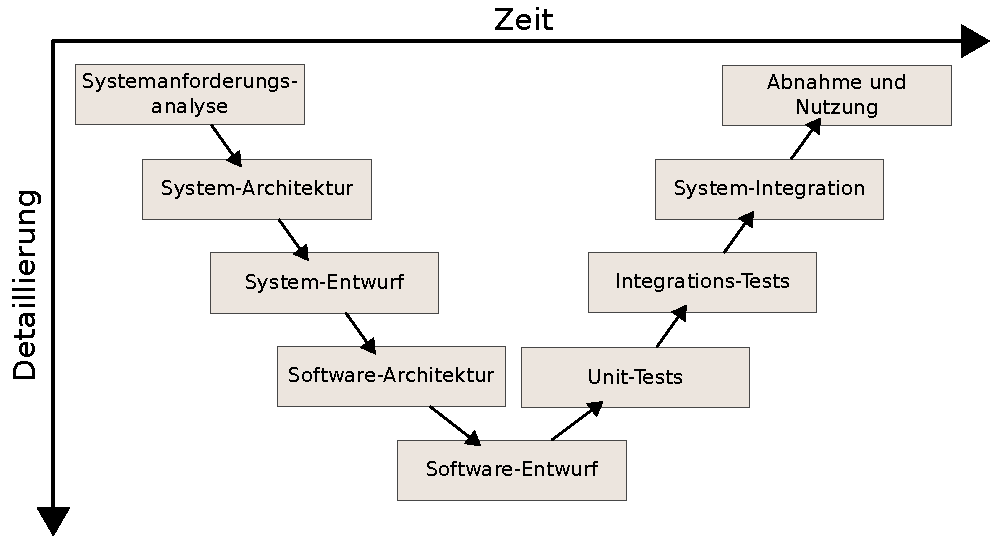
\includegraphics[scale=0.8]{swt2/v-modell.pdf}
		\end{minipage}
\end{itemize}



\section{Agile Entwicklung}

\subsection{Extreme Programming (XP)}
\begin{itemize}
	\item Sammlung aus Werten (Kommunikation, Einfachheit, Feedback, Mut) und Prinzipien (schnelle Lieferung/Feedback, Einfachheit) und Methoden
	\item \textbf{Der Prozess\footnote{\url{http://www.extremeprogramming.org/map/iteration.html}}}\\\\
		\begin{minipage}{\linewidth}
			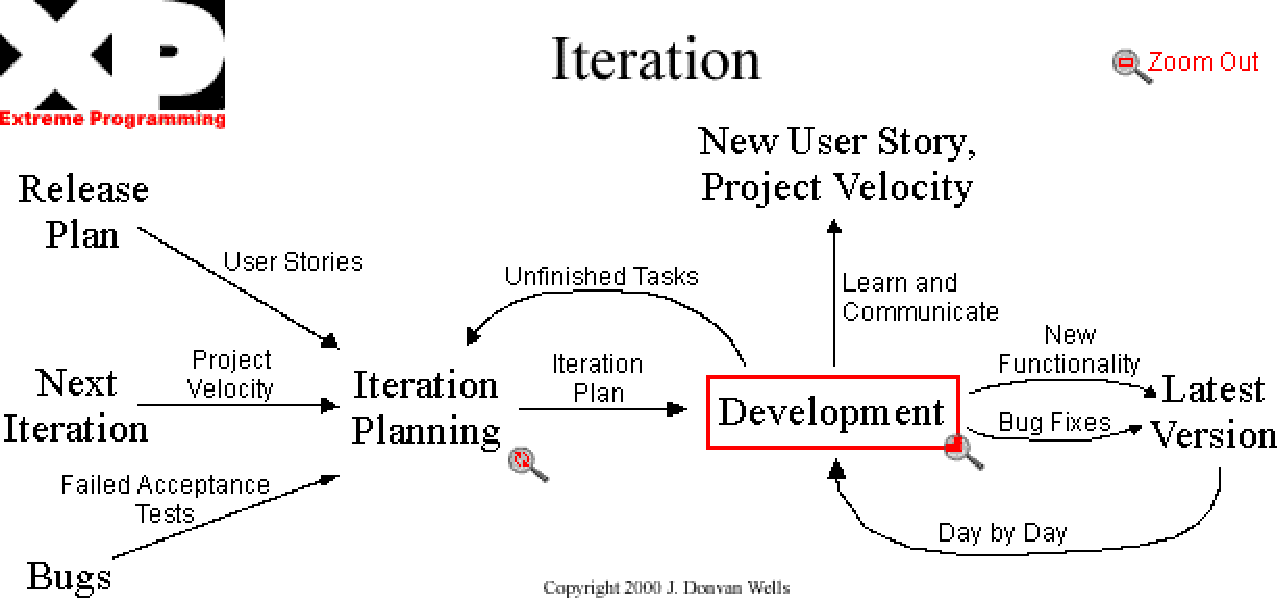
\includegraphics[scale=0.7]{swt2/xp_iteration.pdf}
		\end{minipage}
	\item \textbf{Kritik (allgemein auch an Agile)}
	\begin{itemize}
		\item Schlechte Skalierung bei großen Projekten
		\item Fehlende Dokumentation
		\item Kunden müssen aktiv mitarbeiten
		\item Wirksamkeit mancher Methoden nicht komplett überprüft (beispielsweise Pair-Programming)
	\end{itemize}
\end{itemize}


\subsection{Scrum}
\begin{itemize}
	\item \textbf{Zusammenfassung}
	\begin{itemize}
		\item \textit{Product Owner} erstellt/verwaltet eine priorisierte Liste mit Features, dem \textit{Product Backlog}
		\item Vor jedem \textit{Sprint} entscheidet das \textit{Team} welche Features in diesem \textit{Sprint} umgesetzt werden. Diese werden in den \textit{Sprint Backlog} übernommen
		\item Das \textit{Team} koordiniert die Entwicklung im täglichen \textit{Daily Scrum Meeting}. Der Fortschritt wird in einem Burn-Down-Chart festgehalten
		\item Der \textit{Srum Master} ist für die Kommunikation im \textit{Team} verantwortlich
		\item Während jedem \textit{Sprint} wird ein (möglichst) auslieferungsbereites \textit{Product Increment} erstellt
		\item Letzteres wird vom \textit{Team} im \textit{Sprint Review Meeting} vorgestellt. Anschließend werden im \textit{Retrospective Meeting} mögliche Verbesserungen besprochen
	\end{itemize}
	\item \textbf{Sprints}
	\begin{itemize}
		\item Idealerweise konstante Dauer von höchstens einem Monat
		\item Nach jedem Sprint startet direkt der nächste \(\rightarrow\) der Entwicklungsprozess besteht aus einer Folge von Sprints
		\item Während eines Sprint dürfen keine Änderungen gemacht werden, die das Ziel gefährden oder die Quailität verringern\\\\
		\begin{minipage}{\linewidth}
			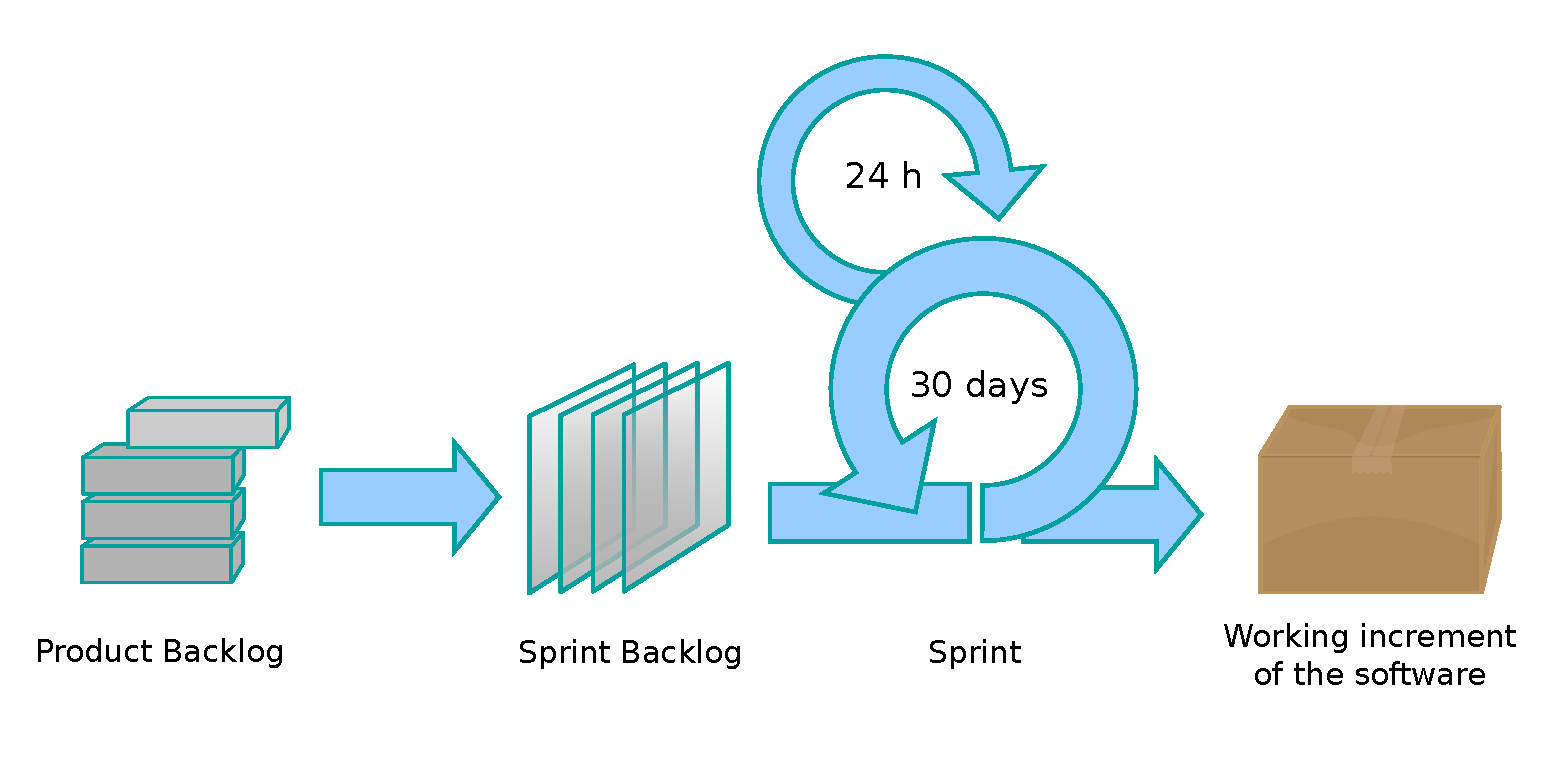
\includegraphics[scale=0.5]{swt2/scrum_process.pdf}
		\end{minipage}
	\end{itemize}
	\item \textbf{Aufgabenverteilung}
	\begin{itemize}
		\item Product Owner
		\begin{itemize}
			\item Repräsentiert den Kunden und ist für den wirtschaftlichen Erfolg des Produkts verantwortlich
			\item Erstellt/priorisiert/erklärt die Produkteigenschaften gegenüber dem Team
			\item Alleinverantwortlich für das Produkt
			\item Typische Fehler: Oft nicht verfügbar, zu wenig Durchsetzungskraft gegenüber unternehmensinternen Stakeholdern oder zu wenig technische Kenntnisse
		\end{itemize}
		\item Scrum Master
		\begin{itemize}
			\item Ist für die Umsetzung von Scrum verantwortlich
			\item Ist für die Kommunikation im Team verantwortlich
			\item Vermittelt gegenüber dem Product Owner
			\item Idealerweise ein Moderator, Coach und erfahrener Softwareentwickler
		\end{itemize}
		\item Team
		\begin{itemize}
			\item Selbstorganisierend, keine vordefinierten Rollen
			\item Idealerweise verschiedene Fachleute (GUI-Designer, Entwickler, Tester, etc.)
			\item Etwa sieben Vollzeitmitarbeiter
		\end{itemize}
		\item Kein klassischer Projektmanager vorhanden. Aufgaben werden von den drei Scrum-Rollen übernommen
	\end{itemize}
	\item \textbf{Product Backlog}
	\begin{itemize}
		\item Liste von Features, die alle Requirements beinhaltet. Nach Geschäftswert sortiert
		\item Jedes Element stellt eine User-Story da und beinhaltet eine Aufwandsangabe (\textit{Story Points})
	\end{itemize}
	\item \textbf{Sprint Backlog}
	\begin{itemize}
		\item User-Stories werden in kleinere Tasks aufgeteilt. Einzelner Task sollte nicht länger als 16 Stunden dauern
		\item Üblicherweise auf einer (non-)virtuellen Pinwand verwaltet \(\rightarrow\) bilden den Sprint Backlog
		\item Verschiedene Zustände pro Task. Beispielsweise: Todo \(\rightarrow\) In Arbeit \(\rightarrow\) Testen \(\rightarrow\) Fertig. Werden bei Zustandsänderung entsprechend verschoben/umgehängt
		\item Problem bei realen Pinwänden: Wissen geht eventuell nach Projektabschluss verloren
	\end{itemize}
	\item \textbf{Tipps für große Projekte}
	\begin{itemize}
		\item Teamgröße: Klein starten und organisch wachsen (siehe Brook's Law)
		\item Abhängigkeiten zwischen Teams verringern
		\item Daily "`Scrum of Scrums"' mit je einem (oder mehreren) Teammitgliedern
	\end{itemize}
	\item \textbf{Tipps für verteilte Teams}
	\begin{itemize}
		\item Nach Möglichkeit vermeiden
		\item Niemals Scrum Master und Team trennen
		\item Teams erst nach Eingewöhnung trennen
	\end{itemize}
\end{itemize}


\subsection{Zusammenfassung Agile Methoden}
\begin{itemize}
	\item Vorteile: Schnelles Feedback sowie reduzierte Risiken; hatte einen großen Einfluss auf Prozessverbesserung in der Industrie
	\item Nachteile: Verwenden der selben Codebasis in verschiedenen Projekten schwierig; Skalierung unklar; hoher Anspruch an die Entwickler; Dokumentation schwierig (Projekte teilweise nur im Code dokumentiert)
	\item Tendenziell Schwächen in Architektur und Design
\end{itemize}



\section{Anforderungsmanagement (Requirements Engineering)}

\subsection{Einführung}
\begin{itemize}
	\item 48 \% aller gescheiterten Softwareprojekte sind an mangelhafter Anforderungsdefinition gescheitert
	\item Beheben von falsch definierten Anforderungen in späteren Entwicklungsphasen kann extrem teuer sein
	\item Beschreibungskriterien: Ausreichend, komplett, widerspruchsfrei, verständlich, eindeutig, überprüfbar, risikoadjustiert
	\item Werden meist in Form von User-Stories (Agile) oder Anwendungsfälle (modellgetrieben) beschrieben
	\item \textbf{Typen von Anforderungen (concern-based Classification)}
	\begin{itemize}
		\item Funktionale Anforderungen (Functional Requirements): Verhalten der Software, beispielsweise bei der Eingabe von Daten; "`kann per Turing-Maschine beschrieben werden"'\footnote{Reussner, andere}
		\item Qualitätsanforderungen (Quality Requirements): Qualitätsmerkmale, beispielsweise Sicherheit, Bedienbarkeit, Performance
		\item Bedingungen (Constraints): Beispielsweise physikalische, rechtliche, kulturelle Umgebung oder Interface (Computerplattform)
	\end{itemize}
	\item Anforderungsingenieur vermittelt zwischen Entwicklern und Benutzern
	\item \textbf{Anforderungsmanagementprozess}
	\begin{enumerate}
		\item Gewinnung unter Einbeziehung sämtlicher Stakeholder
		\item Dokumentation: Anforderungsspezifikation aufstellen
		\item Übereinstimmung: Finden und Aufheben von Konflikten
		\item Überprüfen und Verwalten
	\end{enumerate}
\end{itemize}


\subsection{Techniken zum Finden von Anforderungen}
\begin{itemize}
	\item Fragetechniken: Interviews, Fragebögen, On-Site-Customers
	\item Kreativtechniken: Brainstorming, Perspektivwechsel
	\item Retrospektive Techniken: Systemüberreste, Wiederverwenden, Kokurrenzsysteme
	\item Beobachtungstechniken: Feldbeobachtungen
\end{itemize}

\subsection{Überprüfen ob Anforderungen umgesetzt sind}
\begin{itemize}
	\item Betriebsfähige: Reviews, Tests, formale Beweise
	\item Quantitative: Messen
	\item Qualitative: Keine direkte Prüfung möglich; eventuell (subjektiv) durch Jury
	\item Beschreibende: Reviews
\end{itemize}


\subsection{Grundlegende Beschreibungsempfehlungen}
\begin{itemize}
	\item Problem: Die meisten Anforderungen sind (zu Beginn) in natürlicher Sprache festgehalten
	\item Kurze Sätze, eine Anforderung pro Satz
	\item Festhalten wer für welche Aktionen/Handlungen verantwortlich ist
	\item Führen/Verwenden eines Begriffsglossars
	\item Verwenden einer Satzvorlage
\end{itemize}



\section{Modellgetriebene Entwicklung (Model Driven Development)}
\begin{itemize}
	\item Ziele: Plattformunabhängigkeit; höhere Entwicklungsgeschwindigkeit; bessere Softwarequalität; Wiederverwendbarkeit
	\item Erwartete Vorteile: Kostenreduzierung; kürzere Time-to-Market; variabel
\end{itemize}


\subsection{MDD-Paradigma}
\begin{itemize}
	\item \textit{Domain Expert} künftig für die Entwicklung von Anwendersoftware verantwortlich
	\item Modelle reduzieren die Komplexität, sind (automatisch) analysierbar, verbesseren die Kommunikationseffizienz
	\item \textit{Model-Driven}: Modelle sind primäre Artefakte, anstelle des Sourcecodes.
	\item \textit{Model-Based}: Modelle sind sekundäre Artefakte, die beispielsweise für Dokumentationen erstellt werden
\end{itemize}

\subsubsection{Beispiel: Model Driven Architecture (MDA)}
\begin{itemize}
	\item MDD Implementierung
	\item Bietet Standardisierung
	\item Verwendet existierende Standards
	\item \textbf{Modellformen}
	\begin{itemize}
		\item Computing Independent Models (CIM)
		\begin{itemize}
			\item Umgangssprachliche Beschreibung
			\item Klassendiagramm mit Klassenattributen aber ohne Klassenmethoden
		\end{itemize}
		\item Platform Independent Models (PIM)
		\begin{itemize}
			\item Plattformunabhängiges Modell für Geschäftsprozesse
			\item Hinzufügen von Methoden (und eventuell zusätzlichen, technischen Attributen) zum Klassendiagramm
		\end{itemize}
		\item Platform Specific Models (PSM)
		\begin{itemize}
			\item Plattformabhängiges Modell für Architektur/Services
			\item Ersetzen von generischen Typen durch plattformspezifische
		\end{itemize}
		\item Transformationen (Abstrakte Ebene \(\rightarrow\) Code-Ebene)\\\\
		\begin{tikzpicture}
			\node at (0, 0) [rectangle,draw] (cim)  {\(CIM\)};
			\node at (3, 0) [rectangle,draw] (pim)  {\(PIM\)};
			\node at (6, 0) [rectangle,draw] (psm)  {\(PSM\)};
			\node at (9, 0) [rectangle,draw] (code) {\(Code\)};

			\draw[->] (cim) edge node {} (pim);
			\draw[->] (pim) edge node {} (psm);
			\draw[->] (psm) edge node {} (code);
			\draw[<-] ($(pim.east)!0.5!(psm.west)$) -- ++(0,1cm) node[above] {Plattformmodell}; 
		\end{tikzpicture}
	\end{itemize}
\end{itemize}


\subsection{Schlüsselkonzepte und Definitionen}

\subsubsection{Metamodeling}
\begin{itemize}
	\item Vereinfachtes UML-Klassendiagramm
	\item Müssen immer vollständig sein, d.h. bereits alle Attribute/Typen und Assoziationen/Aggregationen enthalten, da sie automatisch weiterverarbeitet werden
\end{itemize}

\subsubsection{Model Transformation}
\begin{itemize}
	\item Transformation: \texttt{Meta-Model\_A} \(\longrightarrow\) \texttt{Meta-Model\_B} nach vorgegebenen Regeln
\end{itemize}


\subsection{Sprachen und Werkzeuge}
\begin{itemize}
	\item \textbf{Eclipse Modeling Framework (EMF)}
	\begin{itemize}
		\item De-facto MDD-Standard
		\item Wird von vielen großen Firmen und Projekten verwendet
	\end{itemize}
	\item \textbf{Essential Meta-Object Facility (EMOF)}
	\begin{itemize}
		\item Von der \textit{Object Management Group} (OMG) als Metadaten-Architektur definiert
	\end{itemize}
\end{itemize}

% TODO Rest ab Folie #48


\subsection{Forschung und Praxis}



\section{Designpatterns für Enterprise Application Architecture}
\begin{itemize}
	\item \textbf{Eigenschaften von Enterprise Applications (EA)}
	\begin{itemize}
		\item Langlebige Daten: Daten bleiben länger als Anwendungen und Hardware erhalten \(\rightarrow\) müssen in Anwendungen integrierbar sein
		\item Große Datenmengen mit meist mehreren Millionen Datensätzen \(\rightarrow\) effizienter Zugriff notwendig
		\item Konkurrierender Zugriff \(\rightarrow\) Inkonsistenzen müssen verhindert werden
	\end{itemize}
	\item Viele verschiedene Systeme: Shop, Leasing-Management-System, Ausgabenüberwachungssystem
	\item Web Shops: Viele parallele Anwender; einfache Logic
	\item \textbf{Ebenen}
	\begin{itemize}
		\item Präsentation: Benutzerinterface zur Informationsdarstellung und Eingabeverarbeitung
		\item Domain: Logik, Berechnungen
		\item Datenquelle: Kommunikation mit anderen Systemen, beispielsweise Datenbanken
	\end{itemize}
\end{itemize}


\subsection{Patternfamilien}
\begin{itemize}
	\item Jede Familie beschäftigt sich mit einem Problem von EAs
	\item Generell: Kein Pattern ist "`das beste"'. Wahl des Patterns aus einer Familie hängt von den konkreten Vorraussetzungen ab
\end{itemize}

\subsubsection{Domain-Logik Patterns}
\begin{itemize}
	\item Mögliche Herausforderungen: Hohe Komplexität, Austauschbarkeit, Verknüpfung mit Presentation und Datenquelle(n)
	\item \textbf{Pattern: Transaction Script}
	\begin{itemize}
		\item Jede Anfrage wird in einer separaten Prozedur abgearbeitet \(\rightarrow\) sämtliche Transaktionslogik in dieser Prozedur
		\item Beispiel: Laden von Objekt aus der Datenquelle, bearbeiten des Objekts, speichern des Objekts
		\item Vorteile: Einfache, verständliche Prozeduren; unkomplizierte Verbindungen mit Datenquellen; Transaktionsgrenzen einfach feststellbar
		\item Nachteile: Skalieren schlecht bei komplexer Logik; tendenziell doppelter Code
	\end{itemize}
	\item \textbf{Pattern: Domain Model}
	\begin{itemize}
		\item Objektmodell, das Verhalten und Daten beinhaltet
		\item Objekte arbeiten für Transaction zusammen
		\item Vorteil: Bessere Organisation der Domain-Logik
		\item Nachteile: Höhere Ansprüche an Entwickler; Mapping zur Datenquelle komplexer
	\end{itemize}
	\item \textbf{Pattern: Table Module}
	\begin{itemize}
		\item Einzelne Instanz, welche die komplette Logik für eine Tabelle implementiert
		\item Entweder eine Instanz pro Datensatz oder statisch per Singleton
		\item Vorteile: Einfaches Mappen Objekt \(\leftrightarrow\) Tabellenzeile; Logiktrennung für verschiedene Konzepte; nützlich, wenn von bereits verwendeten Technologien unterstützt
		\item Nachteil: Keine Instanzen pro Objekt \(\rightarrow\) eventuell unpraktisch/nachteilig bei komplexen Anwendungen
	\end{itemize}
	\item \textbf{Entscheidungskriterien}
		\item Wichtigstes Kriterium: Komplexität der Domain-Logik
		\begin{itemize}
			\item Bei wenig Komplexität: \texttt{Table Module < Transaction Skript < Domain Model} (gemessen am Implementierungsaufwand)
			\item Bei hoher Komplexität: \texttt{Domain Model < Table Module < Transaction Skript} (gemessen am Implementierungsaufwand)
		\end{itemize}
		\item Wie aufwendig ist das Mapping zur Datenquelle?
		\item Kennen die Entwickler das Domain-Model?
		\item Welche Werkzeuge/Entwicklungsumgebungen werden verwendet?
\end{itemize}

\subsubsection{Datenquelle-Architektur-Patterns}
\begin{itemize}
	\item Ziel: Trennung von Datenbankzugriff und Domain-Logic
	\item Herausforderung: Mapping Objekt \(\leftrightarrow\) Tabellenzeile
	\item \textbf{Pattern: Record Set}
	\begin{itemize}
		\item Lokale (in-memory) Kopie von Tabellenzeile(n)
		\item Einfach zu erzeugen und zu verändern
	\end{itemize}
	\item \textbf{Pattern: Table Data Gateway}
	\begin{itemize}
		\item Ein Objekt als Gateway (nicht als Facade), das den Zugriff auf alle Tabellenzeilen verwaltet
		\item Trennt Anfragen und Datenbankzugriff
		\item Implementiert \textbf{CRUD}-Methoden
		\item Geeignet für \texttt{Transaction Script}, eher ungeeignet für \texttt{Domain Model}
	\end{itemize}
	\item \textbf{Pattern: Active Record}
	\begin{itemize}
		\item Ein Objekt pro Tabellenzeile, das die Datenbankzugriff und Domain-Logic implementiert
		\item Objektorientiert: Vereint Daten und Funktionalität
		\item Mapping muss isomorph sein
		\item Gute Wahl bei wenig komplexer Domain-Logic, ansonsten ungeeignet \(\rightarrow\) \texttt{Data Mapper} verwenden
	\end{itemize}
	\item \textbf{Pattern: Row Data Gateway}
	\begin{itemize}
		\item Objekt, das als Gateway zu einer einzelnen Tabellenzeile fungiert
		\item Idee: Ähnlich wie \texttt{Active Record}, verhindert allerdings die Komplexität; kann SQL-Anfragen für verschiedene Datenbanktypen abstrahieren \(\rightarrow\) alle Zugriffsdetails sind hinter dem Interface versteckt
		\item Meist hat jede Tabelle eine Zusätzliche Finder-Klasse: \texttt{PersonFinder.find(id) \(\rightarrow\) PersonGateway}
		\item Gut geeignet für automatisch erzeugten Zugriffscode (der gesamte Datenbankzugriff wird generiert)
	\end{itemize}
	\item \textbf{Pattern: Identity Map}
	\begin{itemize}
		\item Jedes Objekt wird nur einmal aus der Datenbank geladen und dann lokal im Speicher vorgehalten (Cache)
	\end{itemize}
	\item \textbf{Pattern: Data Mapper}
	\begin{itemize}
		\item Mapping-Layer, der zwischen Datenbank und Objektspeicher vermittelt bzw. diese voneinander isoliert
		\item Mapping kann entweder explizit (für jedes Domain-Objekt existiert ein Mapper) oder Metadaten erfolgt werden, aus denen ggf. Code generiert wird
		\item Beispiel: \texttt{Hibernate}
		\item Verwendung
		\begin{itemize}
			\item Datenbankschema und Objekt-Modell entwickeln sich unabhängig (was meist der Fall ist)
			\item KomplexeBusiness-Logik, \texttt{Active Record} nicht ausreichend
			\item Automatisch erzeugt bei MDD
			\item Legacy Systeme mit bereits existierenden Datenbanken
		\end{itemize}
	\end{itemize}
\end{itemize}

\subsubsection{Sinnvolle Kombinationen aus Datenquelle-Pattern und Domain-Logic-Pattern}
\begin{itemize}
	\item \textbf{Transaction Script}
	\begin{itemize}
		\item \texttt{Row Data Gateway} oder \texttt{Table Data Gateway}
	\end{itemize}
	\item \textbf{Domain Model}
	\begin{itemize}
		\item Wenig komplexes Mapping: \texttt{Active Record}
		\item Komplexes Mapping: \texttt{Data Mapper}
	\end{itemize}
	\item \textbf{Table Module}
	\begin{itemize}
		\item \texttt{Table Data Gateway} (falls RecordSet-Framework)
	\end{itemize}
\end{itemize}

\subsubsection{Object-Relational Structural Patterns}
\begin{itemize}
	\item Mapping von OO-Strukturen zu relationalen Datenbanken (besonders bei \texttt{Domain Model} und \texttt{Data Mapper})
	\item \textbf{Pattern: Single Table Inheritance}
	\begin{itemize}
		\item Verherbungshierarchie mehrerer Klassen wird in einer einzigen Klasse repräsentiert, die Spalten für alle Attribute der verschiedenen Klassen und eine Type-Spalte hat
		\item Vorteile: Einfaches Datenbankschema; keine \texttt{Joins} notwendig; Verschieben von Attributen innerhalb der Hierarchie erfordert kein Anpassen der Tabelle
		\item Nachteile: Viele ungenutzte Attribute; Tabelle kann sehr groß werden; es gibt nur einen Namespace für alle Attribute (problematisch, falls mehrere Klassen gleiche Attributnamen für verschiedene Typen benutzen. Abhilfe: Naming Convention wie beispielsweise \texttt{[Classname]\_[Fieldname]})
	\end{itemize}
	\item \textbf{Pattern: Class Table Inheritance}
	\begin{itemize}
		\item Vererbungshierarchie mit je einer Tabelle pro Klasse
		\item Bei vererbten Klassen werden jeweils lediglich die neuen Attribute in der entsprechenden Tabelle gespeichert
		\item Vorteile: Einfach verständlich; Alle Spalten sind wichtig - keine Speicherverschwendung; einfaches Mapping zwischen Objekt und Datenbank
		\item Nachteile: Beim Laden eines Objekte müssen meist Daten aus mehreren Tabellen geladen werden (Leistungsverlust); aufwendigeres Refactoring; Supertypes können zum Flaschenhals werden
	\end{itemize}
	\item \textbf{Pattern: Concrete Table Inheritance}
	\begin{itemize}
		\item Jede Klasse der Vererbungshierarchie erhält eine Tabelle mit allen (auch den vererbten) Attributen
		\item Vorteile: Einfaches Zugriff, keine überflüssigen Spalten; keine \texttt{Joins} notwendig
		\item Nachteile: Verschieben von Attributen in der Hierarchie erfordert Schemaanpassung; Anpassungen bei Supertypes erfordern viele Änderungen; \texttt{find} über die Superklasse erfordert Suche in allen Subklassen (und damit Subtabellen)
	\end{itemize}
	\item \textbf{Verwendung}
	\begin{itemize}
		\item Alle Pattern in erster Linie zur Verwendung von \texttt{Domain Model} mit \texttt{Data Mapper}
		\item Abwägung zwischen Datendopplung und Geschwindigkeit
		\item Konkrete Wahl hängt von Zugriffsmustern ab
	\end{itemize}
\end{itemize}


\subsection{Praxis: Java Persistance API (JPA)}
\begin{itemize}
	\item Bestandteil von \texttt{Java EE}
	\item Definiert das komplette Mapping zwischen Objekt-Modell und Datenbank
	\item Kann wahlweise per \texttt{Java Annotations} oder \texttt{XML} definiert werden
	\item Vererbungspattern kann explizit festgelegt werden
\end{itemize}



\section{Software Design}

\subsection{Responsibility-Driven Design}
\begin{itemize}
	\item Zentrale Frage: Wie wird die Funktionalität auf die Objekte verteilt?
	\item Software-Objekte sollen tatsächlichen Objekten in der Realität entsprechen
	\item \textbf{Objekte erhalten \textit{Verantwortlichkeiten} (Responsibilities)}
	\begin{itemize}
		\item Doing responsibilities: Für welche Handlungen ist das Objektverantwortlich?
		\item Knowing responsibilities: Welche Informationen hält/teilt das Objekt
	\end{itemize}
	\item Verantwortlichkeiten werden mittels \texttt{Methoden} implementiert
	\item Pattern zum Verteilen von Verantwortlichkeiten: \textit{Informationsexperte}. Verarbeitung erfolgt in dem Objekt, das die Informationen hält
	\item Verarbeitungsbeispiel: Eingabeobjekt wird an die richtige "`Bearbeitungsstelle"' weitergegeben
\end{itemize}


\subsection{Design Diagramme}
\begin{itemize}
	\item Interaktionsdiagramme sind eine große Hilfe beim Entwurf
	\item Aus den fertigen Interaktionsdiagrammen können Software-Klassen abgeleitet werden: Nachricht im Interaktionsdiagramm \(\rightarrow\) Klassenmethode
	\item Typische Bestandteile eines Klassendiagramms: Klassen, Assoziationen, Attribute und deren Typen, Methoden, Interfaces, Abhängigkeiten
\end{itemize}


\subsection{General Responsibility Assignment Software Patterns (GRASP)}
\begin{itemize}
	\item Systematische Beschreibung, welche Objekte für was zuständig sein sollen
	\item \textbf{Creator}
	\begin{itemize}
		\item Legt fest, welches Objekt ein bestimmtes anderes erstellen soll
		\item \texttt{A} erstellt neues Objekt \texttt{B}, falls
		\begin{itemize}
			\item \texttt{A} eine Aggregation von \texttt{B} ist
			\item \texttt{A} \texttt{B}-Objekte beeinhaltet
			\item \texttt{A} \texttt{B}-Objekte mit starker Kopplung verwendet
			\item \texttt{A} die Initialisierungsdaten für \texttt{B} hat
		\end{itemize}
	\end{itemize}
\end{itemize}


\subsection{Zusammenfassung}

\chapter{Telematik}

Zusammenfassung der Vorlesung "`Telematik"' aus dem Wintersemester 2016.\footnote{\url{https://telematics.tm.kit.edu/ws201617_telematik.php}}

\section{Transportprotokolle}

\subsection{Grundlegende Komponenten}

\subsubsection{TCP-Grundlagen}
\begin{itemize}
	\item \textbf{TCP-Verbindungsverwaltung}
	\begin{itemize}
		\item Identifikation einer TCP-Verbindung: Quell-/Zieladresse sowie Quell-/Zielport
		\item Verbindungsaufbau: Server wartet, Client initiiert Verbindung
		\item 3-Wege-Handshake
		\begin{enumerate}
			\item Client \(\rightarrow\) Server: \texttt{TConReq(SYN=1,seq=client\_isn)}
			\item Client \(\leftarrow\) Server: \texttt{TConCnf(SYN=1,ACK=1,seq=server\_isn,ack=client\_isn+1)}
			\item Client \(\rightarrow\) Server: \texttt{ACK(SYN=0,ACK=1,seq=client\_isn+1,ack=server\_isn+1)}
		\end{enumerate}
		\item Zusätzlich: Festlegen der initialen Sequenznummer (\texttt{isn}), Bekanntgabe der Größe des Flusskontrollfensters, Allokation der Puffer
		\item Format einer TCP-Dateneinheit\footnote{\url{https://upload.wikimedia.org/wikipedia/de/f/fd/TCP_Header.svg}}\\
			\begin{minipage}{\linewidth}
				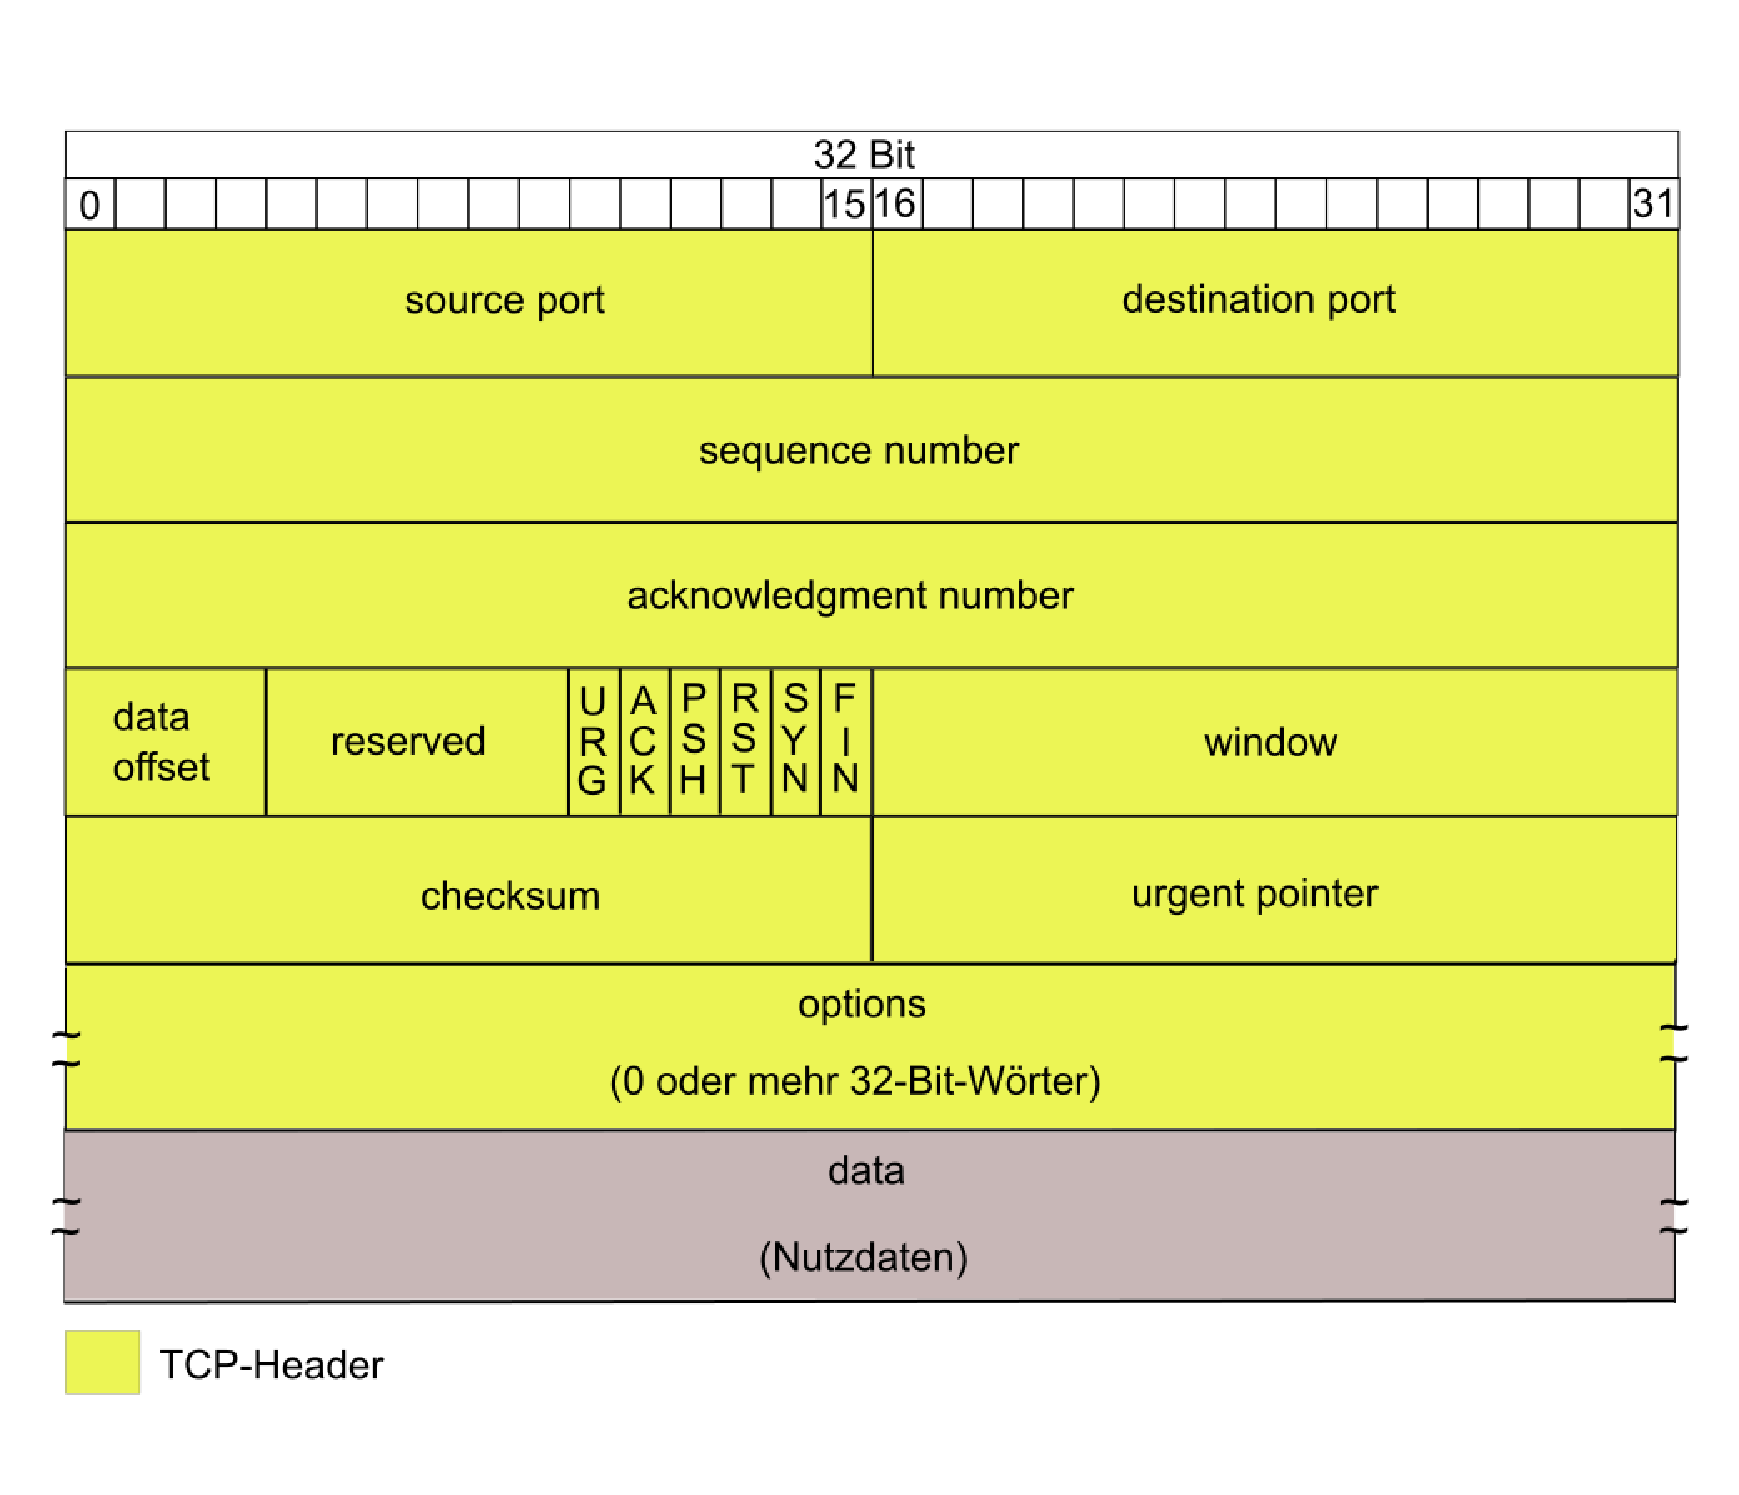
\includegraphics[scale=0.38]{telematik/TCP_Header.pdf}
			\end{minipage}
	\end{itemize}
	\item \textbf{Flusskontrolle zur Schutz des Empfängers vor zu hoher Last}
	\begin{itemize}
		\item Dynamische Anpassung des Empfangsfenster auf Empfängerseite, um die aktuelle verfügbare Puffergröße mitzuteilen. \texttt{RcvWindow} bezeichnet den Anteil des \texttt{RecvBuffer}, das frei ist (jeweils absolute Werte)
		\item Problem: Empfänger meldet ein volles Empfangsfenster. Woher weis der Sender, ab wann er wieder senden darf? \(\rightarrow\) Empfänger muss auch bei vollem Empfangsfenster Dateneinheiten mit einem Byte Länge quittieren (\textit{Zero Window Probing})
	\end{itemize}
	\item \textbf{Angriffe auf den Verbindungsaufbau: SYN-Flooding}
	\begin{itemize}
		\item Massenhaftes Senden von SYN-Dateneinheiten ohne Verbindungsaufbau. Problem: Zustandshaltung auf Empfängerseite für halboffene Verbindungen. Folge: Ressourcen erschöpft, Empfänger kann keine Dateneinheiten mehr annehmen
		\item Lösung: SYN-Cookies
		\begin{itemize}
			\item Verhinderung der Zustandshaltung bis zum letztmöglichen Zeitpunkt: Beginn der Zustandhaltung erst bei Empfang des \texttt{ACK}
			\item Realisierung: Ermittlung der Zustandsinformationen auf Empfängerseite anhand der Informationen aus \texttt{ACK(SYN=0,ACK=1,seq=client\_isn+1,ack=server\_isn+1)}
			\item Kodierungsbeispiel: Zeitstempel zur Verhinderung von Replay-Attacken (5 Bit); ausgewählte MSS aus acht vordefinierten Werten (3 Bit); Hash über Quelladresse und -port sowie Zieladresse und -port, verifiziert dass der Client bereits \texttt{SYN} durchgeführt hat /24 Bit). Daraus entsteht die 32 Bit initiale Sequenznummer des Servers
			\item Nachteil: Vergleichsweise kurze Sequenznummer (32 Bit) reicht nicht für zusätzliche TCP-Optionen und limitiert MSS-Größen auf vordefinierte Werte
			\item Idee: Cookie erst einsetzen, wenn nötig (volle Warteschlange oder Ressourcenengpass)
		\end{itemize}
	\end{itemize}
\end{itemize}

\subsubsection{Staukontrolle}
\begin{itemize}
	\item Beobachtung: Unverhältnismäßiger Leistungseinbruch an Engstellen bei großem Datenaufkommen zwischen zwei schnelleren Netzen \(\rightarrow\) Warteschlangenmanagement notwendig
	\item \textbf{Einfaches Warteschlangenmanagement}
	\begin{itemize}
		\item Puffer im Router voll, nächste Dateneinheit muss verworfen werden ("`Tail Drop"')
		\item Retransmissiontimer im Client steuert Sendewiederholungen
		\item Problem: Synchronisation. Dateineinheiten von mehreren Verbindungen werden quasi gleichzeitig verworfen
	\end{itemize}
	\item \textbf{Aktives Warteschlangenmanagement}
	\begin{itemize}
		\item Das Netz gibt einen Hinweis auf eine entstehende Stausituation, bevor eine Überlast entsteht
		\item Router verwirft (randomisiert) Dateneinheiten, bevor die Warteschlange voll ist. Sorgt für Fairness und verhindert globale Synchronisation
		\item Verfahren
		\begin{itemize}
			\item Konkrete Implementierung: Random Early Detection (RED)
			\begin{itemize}
				\item Wahrscheinlichkeit, dass eine Dateneinheit verworfen wird, steigt linear mit der Warteschlangenlänge
			\end{itemize}
		\end{itemize}
	\end{itemize}
	\item \textbf{Self-Clocking}
	\begin{itemize}
		\item Szenario: Verbindung zweier Netze über langsames Weitverkehrsnetz. Dateneinheiten benötigen bei der langsamen Übertragung mehr Zeit als in den lokalen Netzen. Dadurch kommen sie verzögert beim Empfänger an, welcher sie entsprechend "`langsam"' quittiert. Durch den entstehenden Takt weis der Sender, wie schnell er senden kann. Aber: Wie soll die "`Uhr"' gestartet werden?
		\item Wieso wird trotzdem kein Gleichgewicht erreicht?
		\begin{itemize}
			\item Verbindung kommt nicht ins Gleichgewicht. Mögliche Auslöser: Neue Verbindung/Neustart, automatische Anpassung der Datenrate und Verzögerung
			\item Sender sendet neue Dateneinheiten zu früh
			\item Ressourcenbeschränkungen verhindern Gleichgewicht
		\end{itemize}
	\item \textbf{Slow-Start (Einzelverbindung)}
	\begin{itemize}
		\item Erhöhung der Anzahl der gesendeten Dateneinheiten über die Zeit durch Einführung eines Staukontrollfensters (\texttt{Staukontrollfenster < Flusskontrollfenster}). Verhindert burstartiges Senden der Quelle, was zu vielen Sendewiederholungen führen würde
		\item Bei Verbindungsstart oder Verlust einer Dateneinheit wird das Staukontrollfenster zurückgesetzt
		\item Startverhalten ohne Slow-Start: Viele Sendewiederholungen durch Paketverluste. "`lineares Zickzackwachstum"', das weit hinter der verfügbaren Datenrate zurück bleibt (effektive Nutzung bei 35\%)
		\item Startverhalten mit 2s Slow-Start: Keine Sendewiederholungen, Datenrate nahezu am verfügbaren Maximum. Effiziens abhängig von Vebrindungsdauer, da dann die langsame Slow-Start-Phase an Gewicht verliert
		\end{itemize}
	\end{itemize}
	\item \textbf{Congestion Avoidence (Simultane, konkurrierende Verbindungen)}
	\begin{itemize}
		\item Ohne Congestion Avoidance: Sehr viele Sendewiederholungen (nahezu 50\% im Experiment), sehr unfaire Aufteilung
		\item Mit Congestion Avoidance: Sehr wenige Sendewiederholungen, verschiedene Quittungsstrategien möglich
		\item Zusammenfassung: Faire Aufteilung der verfügbaren Kapazität, langsames Herantasten durch lineares Erhöhen des Staukontrollfensters sowie kaum Sendewiederholungen
	\end{itemize}
	\item \textbf{Fast Retransmit}
	\begin{itemize}
		\item Beobachtung: Nicht jede nicht in Reihenfolge erhaltene Dateneinheit ist ein Indiz für eine Überlastung des Netzes
		\item Mechanismus zur Staukontrolle: Sendewiederholung beim Empfang einer definierten Anzahl duplizierter Quittungen
		\item Vorgehen: Warten auf Timerablauf, dann Sendewiederholung (Wartezeit größer Umlaufzeit \texttt{RTT})
	\end{itemize}
	\item \textbf{Staukontrolle}
	\begin{itemize}
		\item Implizite Staukontrolle: Implizite "`Anzeige"' einer Stausituation ohne explizite Unterstützung des Netzes
		\begin{enumerate}
			\item TCP-Tahoe
			\begin{itemize}
				\item Mechanismen: Slow Start, Timeout, Congestion Avoidance, Fast Retransmit
				\item Nach Timeout oder Empfang duplizirter Quittungen: Beginn von Slow Start
				\item Grundlegende Vorgehensweise: Additives Erhöhen des Congestion Window \texttt{CWnd}, multiplikatives Erniedrigen (\texttt{AIMD})
			\end{itemize}
			\item TCP-Reno
			\begin{itemize}
				\item Zusätzlich zu TCP-Tahoe: Fast Recovery (siehe unten)
				\item Unterscheidet zwischen \textit{schweren Stausituationen} (Timeout bei Ausstehenden Quittungen) und \textit{leichten Stausituationen} (Empfang von duplizierten Quittungen)
				\item Leichte Stausituationen: Kein Rücksetzen auf Slow Start, da Quittungsempfang impliziert, dass weiter neue Daten empfangen worden sind
				\item Schwere Stausituationen: Rücksetzen auf Slow Start wie bei TCP-Tahoe
				\item Fast Recovery
				\begin{itemize}
					\item Szenario: Empfang einer festgelegten Anzahl Quittungen (beispielsweise drei)
					\item Idee: Senden neuer Dateneinheiten, auch wenn der Fehler noch nicht behoben ist (Self-Clocking geht weiter)
					\item Vorgehen: Reduzierung der Belastung (halbieren des Staukontrollfensters) sowie Fast Retransmit
				\end{itemize}
			\end{itemize}
		\end{enumerate}
		\item Explizit Congestion Notification (ECN): Explizite Staukontrolle mit Netzunterstützung
		\begin{itemize}
			\item Idee: Erkennen von Stausituationen im Netz über den Füllstand der Warteschlange (setzt aktives Warteschlangenmanagement voraus) sowie markieren der IP-Einheiten vor Weiterleitung zum Empfänger. Dieser informiert den Sender, um das Staukontrollfenster zu regeln
			\item Signalisierung in Schicht 3 (IP): Nutzung zweier Bits im TOS-Feld der Dateneinheit
			\item Signailisierung in Schicht 4 (TCP): Einführung zusätzlicher Flags im TCP-Kopf
			\begin{itemize}
				\item \texttt{ECE}-Bit: Signalisiert dem Sender die Stausituation (Sender \(\leftarrow)\) Empfänger)
				\item \texttt{CWR}-Bit: Bestätigt dem Empfänger den Erhalt einer Staumeldung (Sender \(rightarrow\) Empfänger)
			\end{itemize}
		\end{itemize}
	\end{itemize}
\end{itemize}

\subsubsection{Fairness}
\begin{itemize}
	\item TCP-Verbindungen konkurrieren um Ressourcen des Netzes \(rightarrow\) faire Aufteilung angestrebt
	\item \textbf{Probleme}
	\begin{itemize}
		\item "`Gierige Nutzer"': Faire Verteilung bezieht sich auf TCP-Verbindungen. Kann daher mehrere Verbindungen gleichzeitig öffnen. Gegenmaßnahme: Verteilung der Kapazität pro Benutzer
		\item "`Gieriger Empfänger"': Da Quittungsverhalten der Empfängerinstanz die Ressourcenzuteilung beeinflusst, kann dieser mehr oder scheller Quittungen senden. Das Staukontrollfenster öffnet sich schneller, damit erhält die Verbindung mehr Ressourcen
		\begin{enumerate}
			\item Mehrere Quittungen pro empfangener Dateneinheit: Sequenznummern zählen Bytes, Staukontrollfenster zählen Dateneinheiten. Bestätigt der Empfänger jede Dateneinheit in mehreren "`Häppchen"', so öffnet sich das Staukontrollfenster schneller
			\item Quittungen schneller senden als Daten empfangen werden. Protokolländerung notwendig
			\item Identische Quittungen mehrfach senden: Fehlende Dateneinheit wird erneut gesendet. Bei TCP-Reno läuft Self-Clocking weiter \(\rightarrow\) Staukontrollfenster wird weiter geöffnet
		\end{enumerate}
	\end{itemize}
\end{itemize}

\subsection{Analyse und Randbedingungen}

\subsubsection{Analyse von TCP: Modelle}
\begin{itemize}
	\item Analytische Beurteilung hinsichtlich Durchsatz und Latenz
	\item Zentrale Fragen: Ist \texttt{TCP} für meine Zwecke geeignet?`Welche Leistung kann ich erwarten?
	\item \texttt{Periodisches Modell}
	\begin{itemize}
		\item Vereinfachte Betrachtung des langfristigen Verhaltens ohne Slow-Start und Sendewiederholungen \(\rightarrow\) Staukontrollfenster bildet "`perfekte"' Sägezahnkurve mit periodischen Paketverlusten
		\item Vorgehen: Berechne die Anzahl übertragender Dateneinheiten \(Y_i\) zwischen zwei aufeinenader folgenden Verlusten von Dateneinheiten (also in einem Durchlauf)
		\item Durchschnittliche Übertragungsrate: \(X=\frac{1}{RTT}\cdot\sqrt{\frac{3}{2p}} = 1,22 \cdot \frac{1}{RTT\cdot\sqrt{p}}\)
		% TODO: mehr?
	\end{itemize}
	\item \texttt{Detaillierstes Verlust-Modell}
	\begin{itemize}
		\item Unterschied zum periodischen Modell: Verluste nicht mehr periodisch \(\rightarrow\) Dauer der Durchläufe nicht mehr gleich lang
		% TODO: mehr?
	\end{itemize}
\end{itemize}

\subsubsection{Hohe Datenraten}

\subsubsection{Kurze Latenzen: TCP und Web}
\begin{itemize}
	\item Interaktiver Dienst, Besucher äußerst ungeduldig \(\rightarrow\) Antwortzeit entscheident
	\item Verwendung von \texttt{HTTP} in \texttt{TCP} \(\rightarrow\) bei jedem Klick/pro Objekt wird mindestens eine \texttt{TCP}-Verbindung aufgebaut \(\rightarrow\) sehr viele Verbindungsaufbauten für wenig Übertragung
	\item Bei kleinen Objekten dominieren RTTs die Antwortzeit; Slow-Start hat entscheidenden Einfluss auf die Verzögerung
	\item \textbf{Möglichkeiten zur Verbesserung}
	\begin{itemize}
		\item Größeres initiales Staukontrollfenster: Mindestens 10 \texttt{TCP}-Segmente mit \(\sim 15\) KByte, da 90\% aller Web-Objekte \(\le 16\) KByte sind. Google-Messungen (in kleiner Umgebung) bestätigen die Vermutung, wobei das initiale Staukontrollfenster auch nicht zu groß werden darf
		\item TCP-Fast-Open (TFO): Verzögerungsreduzierung beim Verbindungsaufbau, in dem bereits im \texttt{SYN}-Paket Daten ausgeliefert werden, die allerdings erst nach dem kompletten Handshake an die Anwendung ausgeliefert werden \(\rightarrow\) verkürzt die Latenz um eine \texttt{RTT}, eröffnet aber auch die Möglichkeit für DoS-Attacken mittels \texttt{SYN}-Flooding \(\rightarrow\) TFO-Cookie als mögliche Lösung
	\end{itemize}
\end{itemize}


\subsection{Aktuelle Entwicklungen}

\subsubsection{Realität im Internet}
\begin{itemize}
	\item Datentransport nicht mehr nur klassischerweise zwischen Endgeräten, die über Routern kommunizieren. Paradigma: \texttt{IP}-Dateneinheiten wirden nicht modifiziert \(\rightarrow\) beliebige Transportprotokolle nutzbar
	\item Praktisch greifen jede Menge Middleboxes in den E2E-Datenstrom ein und können fast alle Felder einer \texttt{TCP}-Dateneinheit verändern \(\rightarrow\) keine E2E-Transparenz mehr. Beispiele: Physikalische (Hardware-Firewall) oder virtuelle (NAT in Heimroutern, Software-Firewall) Einheiten. Datenpfade ohne Middleboxes eher die Ausnahme
	\item Network Address Translation (NAT) für maskierte Netze. NAT-Router ersetzt ausgehende Pakete durch seine Adresse und speichert das Mapping zum Zuordnen von Antworten. NAT-Router muss hierfür das Transportprotokoll kennen
	\item \textbf{Firewall}
	\begin{itemize}
		\item Untersuchen Dateneinheiten nach konfigurierten Regeln und verwerfen diese ggf.
		\item \textit{Shallow Packet Insepction}: Bewertung anhand des \texttt{IP}-Kopfs und den Köpfen der Transportprotokolle
		\item \textit{Deep Packet Inspection}: Anwendungsorientierte Bewertung, beispielsweise das Erkennen und Blockieren von Malware
	\end{itemize}
	\item \textbf{Proxy}
	\begin{itemize}
		\item Führen Kommunikation an statt des Clients durch
		\item Können Ressourcen zwischenspeichern; Anfragen ablehnen/verändern; Logs anlegen
		\item Häufig: Sperren mittels Firewalls, Erlauben mittels Proxys
		\item Nicht-transparent (kann sich Servern gegenüber zu erkennen geben) oder transparent (benötigt Unterstützung der Netzwerkinfrastruktur, häufig zur Überwachung eingesetzt)
	\end{itemize}
	\item \textbf{Load-Balancer}
	\begin{itemize}
		\item Verteilt Anfragen/Berechnungen auf verschiedene, nachgelagerte Server, oft kombiniert mit vorgelagerten Caches
		\item Erscheint als Ziel-Adresse eines Services ("`umgedrehtes"' NAT)
	\end{itemize}
	\item Cache: Schnelle Auslieferung häufig angefragter Daten, oft in Kombination mit einem Proxy
	\item \textit{Head-of-Line Blocking}: Zuverlässiger Transportdienst blockiert auf Grund von fehlenden Dateneinheiten (Reihenfolgetreue) \(\rightarrow\) Daten werden nicht an Anwendung ausgeliefert. Bei Multimediakommunikation und im Web nicht erwünscht (interaktiver Dienst, Antwortzeit entscheident)
	\item \textbf{SPDY und HTTP/2}
	\begin{itemize}
		\item \texttt{SPDY} zunächst von Google zum teilweise Ersetzen von \texttt{HTTP} (Weiterentwicklung durch \texttt{IETF} zu \texttt{HTTP/2})
		\item Ziele
		\begin{itemize}
			\item Kurze Antwortzeiten: Eine dauerhafte \texttt{TCP}-Verbindung pro Server; Priorisierung von Anfragen; Server-Push; effizientere Header-Kodierung (verienfacht, binär und komprimiert)
			\item Verbesserte Sicherheit: \texttt{TLS} verpflichtend 
			\item Rückwärtskompatibilität
		\end{itemize}
		\item Probleme: Kleine initiale Staukontrollfenster behindern \texttt{SPDY}; Slow-Start-After-Idle ruiniert Langzeitverbindungen; Head-of-Line Blocking durch verlorene Dateneinheiten
	\end{itemize}
	\item \textbf{Quick UDP Internet Onnections (QUIC)}
	\begin{itemize}
		\item Ziele: Vermeidung von Head-of-Line Blocking; Reduzierung der \texttt{RTT}
		\item Einbettung zwischen \texttt{UDP} und \texttt{SPDY} bzw. \texttt{HTTP/2}
		\item Wichtige Eigenschaften: Schneller (\texttt{0-RTT}) Verbindungsaufbau; Vorwärtsfehlerkorrektur auf Ebene der Dateneinheiten; eigene Staukontrolle
	\end{itemize}
\end{itemize}

\subsubsection{TCP in Datenzentren}
\begin{itemize}
	\item Extrem hohe Anforderungen an Leistungsfähigkeit der Kommunikationssysteme; häufig Nutzung von Commodity-Netzen; Fat-Tree-Topologie (siehe Datacenter-Ethernet)
	\item \textbf{Typische Eigenschaften}
	\begin{itemize}
		\item Geringe Umlaufzeit durch geografische Nähe
		\item Incast-Kommunikation (Many-To-One): Mehrere Quellen senden zu einer Senke. Beim parallelen Laden zusammenhängender Daten bestimmt die langsamste Verbindung die Geschwindigkeit (Barrier Synchronization) \(\rightarrow\) Staugefahr am Switch
		\item Multiple Paths zwischen Servern
		\item Mischung von langen und kurzen Flows
		\item Virtualisierung
	\end{itemize}
	\item Data-Center-TCP: Konstant kurze Warteschlangen bei Switches durch \texttt{ECN} imd reduzierte Staukontrollfenster beim Sender
\end{itemize}

\subsubsection{Multipath-TCP (MPTCP)}
\begin{itemize}
	\item \textbf{Motivation}
	\begin{itemize}
		\item Mobile Geräte haben typischerweise mehrere Netzwerkgeräte (WLAN, Ethernet, 3G, etc.); redundante Pfade in Datenzentren; Multi-Homing für Serverfarmen \(\rightarrow\) \texttt{TCP}-Verbindungen sollten zwischen Netzwerkgeräten migriert werden können
		\item \texttt{TCP} ist durch statische Identifikation (Adressen, Ports) ein \textit{Single-Path Protokoll}
	\end{itemize}
	\item Ziel: \texttt{TCP} zur Nutzung mehrerer Pfade erweitern; Anwendungskompatibilität und Netzwerkompatibilität sollen erhalten bleiben
	\item Herausforderung: Middleboxen, die Zustände halten
	\item \textbf{Architektur}
	\begin{description}
		\item{\texttt{MPTCP}-Verbindung}: E2E-Kommunikationsbeziehung; besitzt ein oder mehrere \texttt{MPTCP}-Subflows
		\item{\texttt{MPTCP}-Subflow}: Ein konkreter Pfad; entspricht einer "`regulären"' \texttt{TCP}-Verbindung; können dynamisch zu einer \texttt{MPTCP}-Verbindung hinzugefügt/gelöscht werden
		\item{OSI-Schicht}: Neue Subschicht oberhalb von \texttt{TCP} ("`Manegement der Multipath-Verbindung"')
	\end{description}
	\item Weitere Details: Ein Gesamt-Eingangspuffer für alle Subflows; Subflow-Scheduling; Subflow-Staukontrolle
\end{itemize}



\section{Routing im Internet}

\subsection{Grundlagen}
\begin{itemize}
	\item Aufgaben: Weiterleitung sowie Kopplung von Netzen \(\rightarrow\) Verknüpfung einzelner Übertragungsabschnitte zu einer E2E-Übertragung
	\item Wegfindung im Kommunikationssystem: Weiterleitung im Router anhand Weiterleitungstabelle. Schnelle Weiterleitung mittels kurzen Warteschlangen und kleinen Tabellen
	\begin{itemize}
		\item Pro Dateneinheit ein Lookup in Weiterleitungstabelle
		\item \textit{Metriken} (üblicherweise Ganzzahl) zur Bewertung von Übertragungsabschnitten
		\item \textit{Policies} als Betreibervorgabe zur Routingstrategie. Bsp.: Bevorzugt bestimmten Nachbarn wählen
	\end{itemize}
	\item Herausforderung: Weiterleitung in Line-Speed. Dazu extrem teure, spezielle Cisco Hardware mit bis zu \texttt{1,2 Tbit/s} pro Chassi \(\rightarrow\) nur wenige dutzend Nanosekunden Bearbeitungszeit pro Dateneinheit
	\item Das Internet Protokoll (IP): Unzuverlässiger Dienst; keine Kontexthaltung in Zwischensystemen; keine Verbindungen
\end{itemize}

\subsubsection{Router}
\begin{itemize}
	\item \textbf{Weiterleitung}
	\begin{itemize}
		\item Aufbau Weiterleitungstabelle: \(Prefix \rightarrow Port\) mit Default-Regel am Ende (falls keine der oberen Regeln zutrifft)
		\item Falls mehrere Einträge passen: \textit{Longest Prefix Matching}
		\item Suche in Line-Speed: Verfahren
		\begin{itemize}
			\item Binärer Trie: Pfadabstieg entsprechend den Adressbits
			\item Patricia Trie zur kombrimierten Speicherung von Binärbäumen: Knoten ohne Verzweigung überspringen und dabei Index vom nächsten relevanten Bit merken
			\item Problem bei Bäumen: Eintrag im Worst-Case erst nach \(N=Adress\_Laenge\) Schritten gefunden
			\item Hash-Tabelle zur Beschleunigung des Lookups
			\begin{itemize}
				\item Longest-Prefix nicht praktikabel \(\rightarrow\) Suche nach der kompletten Adresse
				\item Trie-Lookups lediglich, wenn kein Eintrag in der Hashtabelle vorhanden ist
			\end{itemize}
			\item Hardwarerealisierung \textit{Content-Addressable Memory} (CAM)
			\begin{itemize}
				\item Speicherzugriff über einen Teil des gespeicherten Inhalts
				\item Sehr schnell, da in Hardware realisiert; paralleler Zugriff möglich
				\item Anwendung hier: Abbildung \(IPAdresse \rightarrow Ausgangsport\)
				\item Problem: Zuordnung einzlner Adressen wenig hilfreich. Daher \textit{Ternary Content-Addressable Memory} mit dont-care Bits \(\rightarrow\) Suche nach Präfixen möglich
			\end{itemize}
		\end{itemize}
		\item Aufgaben bei Weiterleitung: Header überprüfen; TTL aktualisieren; Prüfsumme neu berechnen; Lookup; Fragmentierung; Behandlung von IP-Optionen; ggf. Klassifizierung und Priorisierung
		\item Generische Router-Architektur: Der Routingprozessor behandelt lediglich die Kontrolldateneinheiten. Alle Komponenten außer der Routingprozessor puffern. Zielkonflikt Leistungsfähigkeit vs. Kosten\\\\
		\begin{figure}[!h]
		\centering
		\begin{tikzpicture}
			\node at (4, -3)    [rectangle,draw,minimum height=4cm,minimum width=3cm] (sf)  {Switch-Fabric};
			\node at (4,  0)    [rectangle,draw,minimum height=1cm,minimum width=3cm] (rp)  {Routing-Prozessor};
			\node at (0, -1.5)  [rectangle,draw,minimum height=1cm,minimum width=3cm] (e1)  {Lookup \& Weiterleiten};
			\node at (0, -4.5)  [rectangle,draw,minimum height=1cm,minimum width=3cm] (en)  {Lookup \& Weiterleiten};
			\node at (8, -1.5)  [rectangle,draw,minimum height=1cm,minimum width=3cm] (a1)  {};
			\node at (8, -4.5)  [rectangle,draw,minimum height=1cm,minimum width=3cm] (an)  {};

			\node at (0, 0) {\textbf{Eingangsports}}; \node at (8, 0) {\textbf{Ausgangsports}};
			\node at (0, -3) {\(\vdots\)}; \node at (8, -3) {\(\vdots\)};

			\draw[<->] (sf) edge node {} (rp);
			\draw[-] (e1.west) -- ++(-0.5cm,0) |- (e1); \draw[->] (e1) edge node {} (e1-|sf.west);
			\draw[-] (en.west) -- ++(-0.5cm,0) |- (en); \draw[->] (en) edge node {} (en-|sf.west);
			\draw[-] (sf.east|-a1) edge node {} (a1);   \draw[->] (a1) -| (a1.east) -- ++(0.5cm,0);
			\draw[-] (sf.east|-an) edge node {} (an);   \draw[->] (an) -| (an.east) -- ++(0.5cm,0);
		\end{tikzpicture}
		\end{figure}
	\end{itemize}
	\item \textbf{Switch-Fabric}
	\begin{itemize}
		\item Blockierungen: Gegenmaßnahmen
		\begin{itemize}
			\item \textit{Overprovisioning}: Interne Verbindungen schneller als Eingangsports
			\item Pufferung an den Netzwerkschnittstellen und in Switch-Fabric
			\begin{itemize}
				\item Annahmen zur Vereinfachung: Gleiche Datenrate an allen Ports; alle Pakete gleich groß
				\item Eingangspuffer: Konfliktauflösung am Eingang; geeignete Scheduling-Strategie
				\item Ausgangspuffer: Konfliktauflösung am Ausgang, allerdings \(N\)-fache Vermittlungsgeschwindigkeit der Eingangsports notwendig. Kurze Eingangspuffer zur Aufnahme von jeweils einer Dateneinheit trotzdem notwendig
				\item Verteilter Puffer pro Knotenpunkt in Switch-Fabric: Höherer Speicherbedarf
				\item Zentraler Puffer zur Konflikauflösung: Geringerer Speicher als bei den anderen Puffern nötig, allerfings höhere Anforderungen an die Speicherzugriffszeit 
			\end{itemize}
			\item Backpressur: Überlastsignalisierung an den Eingangsports \(\rightarrow\) Eingangsports reduzieren Last
			\item Parallele Switch-Fabrics
		\end{itemize}
		\item Struktur der Switch-Fabric
		\begin{itemize}
			\item Gemeinsamer Speicher
			\item Bus-/Ringstruktur: Konfliktfreier Zugriff durch Zeitmultiplex; \(Uebertragungskapazitaet \ge \sum Kapazitaet-Eingangsport_i\); Multicast und Broadcast trivial; Anzahl der Anschlüsse sehr begrenzt (\(\le 16\)); Bsp.: \texttt{CISCO 7500}
			\item Koppelmatrix: Alle Eingänge mit alles Ausgängen verbunden; teilweise parallel nutzbar; hoher Verdrahtungsaufwand; unflexibel; besonders effizient bei gleichgroßen Dateneinheiten
			\item Mehrstufige Verbindungsnetzwerke: Ebenfalls alle Eingänge mit allen Ausgängen durch hierarchische Schaltelemente verbunden; geringerer Verdrahtungsaufwand als Koppelmatrix; nicht alle Verbindungen gleichzeitig möglich
		\end{itemize}
	\end{itemize}
\end{itemize}

\subsubsection{Routing-Algorithmen}
\begin{itemize}
	\item Kontrollpfad: Austausch von Routingnachrichten zur Berechnung von Wegen; Routingprotokolle
	\item Datenpfad: Weiterleitung von IP-Paketen
	\item Routingtabelle: \(Prefix \rightarrow Next~Hop\); wird von den Routingalgorithmen erstellt; auf die Anforderungen von Routingalgorithmen optimiert
	\item Weiterleitungstabelle: \(Prefix \rightarrow Ausgangsport\); auf effizienten Lookup optimiert
	\item \textbf{Verteiltes Adaptives Routing}
	\begin{itemize}
		\item Router reagieren denzentral auf sich ändernde Netzsituation (Laständerungen, Linkfehler, etc.)
		\item Adaptiv: Verteiltes Routing mit Informationsaustausch zwischen den Routern
		\item Benötigte Komponenten: Monitoring, Informationsaustausch, Berechnung aktueller/alternativer Routen
	\end{itemize}
	\item \textbf{Distanzvektor vs. Link-State}
	\begin{itemize}
		\item Distanzvektor-Algorithmus: Iterative Berechnung der kürzesten Pfade (beispielsweise via Bellman-Ford-Algorithmus). Umsetzung als \textit{Router Information Protocol} (RIP) im Internet. Routinginformationen werden auf Basis der Informationen von den Nachbarn berechnet und ausgetauscht
		\item Link-State-Algorithmus: Globale Sicht zur Berechnung der kürzesten (Dijkstra-Algorithmus) \(\rightarrow\) jeder Router muss alle Links im Netz kennen \(\rightarrow\) Informationen über lokale Links eines Routers breiten sich im gesamten Netz aus; jeder ROuter berechnet kürzeste Wege selbstständig (replizierte Berechnung)
	\end{itemize}
\end{itemize}

\subsubsection{Routing-Architektur}
\begin{itemize}
	\item Strukturierung in \textit{Autonome Systeme} mit externem (\texttt{Exterior Gateway Protocol}) und internem (\texttt{Interior Gateway Protocol}) Routing \(\rightarrow\) Skalierbarkeit durch zwei logische Ebenen
	\item Autonome Systeme: Erscheinen nach außen als Einheit mit einheitlichem internen Routingprotokoll und gleicherer internen Routingpolicy. IANA delegiert die Zeitteilung
	\begin{itemize}
		\item Aufteilung nach Funktion: Stub-AS (kleines Unternehmen mit einem Provider); Multihomed AS (große Unternehmen mit mehreren Providern); Transit AS (Provider)
		\item Aufteilung nach Bedeutung: Transit AS/Tier-1 mit angeschlossenen Tier-2-Ebenen, etc.
	\end{itemize}
	\item Transit: Ziel ist Übertragungspfade zu allen am Internet teilnehmenden ASen herstellen. AS-Betreiber kauft hierzu die Konnektivität zu einem/mehrerer ASen ("`Durchgangsverkehr"' zu ASen, die nicht direkt angeschlossen werden können)
	\item \textbf{Peering}
	\begin{itemize}
		\item Private Peering: Direktverbindung zweier ASe i.d.R. auf gleicher Ebene mit kostenneutralen Datenaustausch ohne Transitverkehr anderer ASe \(\rightarrow\) Einsparung von Transitkosten, da beide ASe profitieren. Sehr komplex durch unterschiedliche geografische Standorte
		\item Public Peering über \textit{Internet Exchange Points} (IXPs): Neutrale Durchleitung auf Schicht 2; keine Unterscheidung nach Kunde, Inhalt oder Diensttyp. Beispiel: \texttt{DE-CIX} in Frankfurt mit mehreren \texttt{TB/s} Datenaufkommen
	\end{itemize}
	\textbf{Einteilung Autonomer Systeme}
	\begin{description}
		\item{Tier-1}: Größte globale ASe mit Peering zu allen anderen ASen; Verkauf von Transit. Beispiele: Level3, AT\&T, Sprint
		\item{Tier-2}: Große, überregionale ASe für Verbindungen zu Anbietern von Internet-Anwendungen; Verkaufen Transit und betreiben i.d.R. Peering. Beispiele: Vodafone, Comcast, Tele2
		\item{Tier-3}: Kleinere, regionale ASe; Kaufen Transit von Tier-2-ASen, verkaufen Transit an Endanwender und betreiben i.d.R. Peering. Beispiele: KabelBW, Congstar, Versatel
	\end{description}
	\item \textbf{Content-Delivery-Network (CDN)}
	\begin{itemize}
		\item Performante Bereitstellung von Inhalten mit niedrigen Latenzen \(\rightarrow\) Lokation in Tier-1-Nähe wünschenswert
		\item Webserver direkt über eigene Router verbunden. Peering mit wichtigen Providern wie Google oder Yahoo
		\item CDN-internes Loadbalancing über die Access-Router
	\end{itemize}
\end{itemize}


\subsection{Routing-Protokolle}

\subsubsection{Interior Gateway Protocol (IGP)}
\begin{itemize}
	\item \textbf{Routing Information Protocol (RIP)}
	\begin{itemize}
		\item Eines der ersten Routingprotokolle im Internet. Sehr einfach mit wenig Konfigurationsaufwand
		\item Jeder Router kennt nur seine Nachbarn und die Links zu diesen. Periodisches Versenden (Advertisements, 30s-Takt) von Routinginformationen über UDP. Eine Route wird ungültig, wenn sie nach 180s nicht aufgefrischt worden ist (Wert wird auf \(unendlich\) gesetzt)
		\item Lokal berechnete kürzeste Pfade werden an die direkten Nachbarn weitergeleitet \(\rightarrow\) Routen werden im Netz propagiert
		\item \(Distance \in \{1,\dots,15\}\) entspricht der Hop-Anzahl zum Ziel. \(Distance=16\) entspricht "`unendlich"'
		\item Verhalten bei eingehenden Routingnachrichten: Hinzufügen (wenn nicht vorhanden und Metrik nicht \(unendlich\)) oder aktualisieren (falls neue Route besser ist)
		\item Spalten der Routingtabelle: \texttt{Zielnetz}, \texttt{Nächster Router}, \texttt{Anzahl Hops}
		\item Spalten einer Routingnachrichtstabelle: \texttt{Zielnetz}, \texttt{Anzahl Hops}
	\end{itemize}
	\item \textbf{Open Shortest Path First (OSPF)}
	\begin{itemize}
		\item Link-State-Protokoll mit globaler Netzwerksicht \(\rightarrow\) alle Router benötigen eine globale Sicht (abgelegt in Link-State-Datenbank)
		\item Arbeitet direkt oberhalb von \texttt{IP} ohne zwischengelagertes Transportprotokoll
		\item Sychronisierung der Link-State-Database sobald sich zwei benachbarte Router kennenlernen; im weiter Verlauf lediglich Austausch von Updates
		\item Flooding-Protokoll für Routing-Updates per Multicast mit Sequenznummer an alle direkten Nachbarn (Nachbarn aktualisieren nur, wenn Route neu oder besser mit neueren Sequenznummer)
		\item Vermeidung von redundanten Informationsfluten bei Routingupdate: Explizite Auswahl eines \textit{Designated Router} (DR), der die Signalisierungsaufgabe übernimmt
		\item Sicherung der Zuverlässigkeit der Routing-Updates: Pro-Hop-Quittungen mit Zeitgeber und Prüfsummen. Zusätzlich Authentifizierung möglich (beispielsweise durch IPSec auf IP-Ebene)
		\item Format einer Routing-Nachricht: Header inklusive Anzahl an Updates (\textit{Link State Advertisements} LSAs)) mit den LSAs
		\item OSPF-Router müssen ihr direkten Nachbarn kennen (um Updates zu empfangen und den Zustand der Übertragungsabschnitte bestimmen zu können): Periodische Hello-Nachrichten an die Multicast-Adresse \texttt{224.0.0.5} ("`AllOSPFRouters"') \(\rightarrow\) Prüfen ob der Übertragungsabschnitt korrekt funktioniert sowie Auswahl eines zuständigen Routers für den Übertragungsabschnitt
		\item Skalierbarkeit wird durch zusätzliche Hierarchie-Ebene erreicht: Router werden in Gruppen eingeteilt: "`OSPF-Areas"' und diese durch \textit{Area Border Router} verbunden. Alle anderen Router einer Area kommunizieren lediglich mit Routern innerhalb der Area
		\item Abwärtskompatibel zu \texttt{RIP}
		\item Traffic-Engineering durch Type-of-Service-Headerfeld möglich
	\end{itemize}
	\item \textbf{Vergleich/Zusammenfassung}
	\begin{itemize}
		\item \texttt{RIP}: Begrenzte Möglichkeiten (nur eine Metrik, maximale Pfadlänge auf 15 begrenzt); periodische Updates ggf. ohne Änderungen; konvergiert langsam; Count-to-Infinity \(\rightarrow\) für große Netze ungeeignet
		\item \texttt{OSPF}: Behebt \texttt{RIP}-Probleme (konvergiert schnell, zyklenfrei, geringerer Signalisierungsaufwand); zusätzliche Hierarchieebene; \texttt{RIP}-Geräte können am Rand des NEtzwerks eingebunden werden
	\end{itemize}
\end{itemize}

\subsubsection{Exterior Gateway Protocols (EGP): Border Gateway Protokoll (BGP)}
\begin{itemize}
	\item Weltweiter Einsatz als Basis des heutigen weltweiten Internetroutings zwischen Autonomen Systemen
	\item Erweitertes Pfad-Vektor-Protokoll: Verbreitung von Pfaden statt Metriken \(\rightarrow\) garantiert Schleifenfreiheit
	\item Entscheident für die Wegewahl: Netzbetreiberpolicies (hinsichtlich Wirtschaftlichkeit oder vertraglichen Vereinbarungen)
	\item Einsparung von Routingnachrichten durch geschickte Präfixvergabe (Zusammenfassen von Adressbereichen)
	\item \textbf{Zusammenspiel von BGP und IGPs}
	\begin{itemize}
		\item Default-Route für unbekannte/externe Ziele zum nächsten BGP-Router. Nicht praktikabel für Transitverkehr
		\item Veröffentlichung von externen Routen über IGP
		\item IGP-Router auch BGP sprechen lassen. Oft bei großen Backbone-Providern der Fall
	\end{itemize}
	\item BGP-Sessions über TCP-Verbindungen. Routing dabei über IBGP oder über direkte physische Verbindungen (kein Routing nötig) oder manuell konfiguriert. Nachbarn werden \textit{Peers} genannt
	\item \textbf{Nachrichtentypen}
	\begin{itemize}
		\item \texttt{OPEN}: Aufbau einer Verbindung zum Peer. TCP-Verbindung muss bereits bestehen
		\item \texttt{UPDATE}: Bekanntgabe eines neuen, besseren Pfads, Rücknahme eines veralteten Pfads
		\item \texttt{KEEPALIVE}: Quittung zu einem \texttt{OPEN}-Request zum Aufrechterhalten der Verbindung
		\item \texttt{NOTIFICATION}: Fehlermeldungen oder Verbindungsabbau
	\end{itemize}
	\item \textbf{Routing}
	\begin{itemize}
		\item Kein Mechanismus zur Pfadwahl vorgegeben: Policies entscheident
		\item \textit{Routing Information Base} (RIB) zur Verwaltung der Routen
		\item Verarbeitung von Updates: \textit{Input Policy Engine} \(\rightarrow\) \textit{Entscheidungsprozess} \(\rightarrow\) \textit{RIB} \(\rightarrow\) \textit{Output Policy Engine}
		\item Neben der eigentlichen Routingtabelle werden die empfangen/versendeten Routen pro eingehendem/ausgehenden Peer gespeichert
	\end{itemize}
	\item Herausforderungen: Aufrechterhalten der Skalierbarkeit (Tabellenwachstum, Dynamik der Routingänderungen); Sicherheitprobleme
	\item \textbf{Multi-Homing}
	\begin{itemize}
		\item AS am Rand des Internets wird über mehrere ASe an das Internet angeschlossen
		\item Vorteile: Ausfallsicherheit; Verteilungsmöglichkeiten (wichtiger Verkehr über teuren Uplink, restlicher über günstigen)
		\item Nachteil: Aggregierung von Präfixen wird aufgebrochen \(\rightarrow\) Routenänderungen müssen schlimmstenfalls im ganzen Internet propagiert werden. Abhilfe möglicherweise \texttt{NOPEER}-Attribut: Schränkt die Propagierung von Änderungen am Rand des Internets ein
	\end{itemize}
	\item Exponentielles Größenwachstum der Routingtabellen durch zunehmendes Multi-Homing und Verkehrslastsenkung über BGP, da viele kleine Präfixe propagiert werden \(\rightarrow\) zunehmende Dynamik der Routen
	\item Route Flap Damping: Temporäres Unterdrücken von instabilen Routen durch Erhöhen eines Strafwertes pro Update. Strafwert fällt exponentiell wieder ab. Wird ein bestimmter Wert überschritten, werden die Updates unterdrückt. Kann zu Konnektivitätsverlust kommen
	\item \textbf{Sicherheit des Inter-Domain-Routings}
	\begin{itemize}
		\item Probleme: Netzbetreiber verdienen mit der Bekanntgabe von Routinginformationen Geld; wie können die übermittelten Informationen geschützt werden?
		\item Verschiedene Lösungsansätze verschiedener Hersteller zur Sicherung der Übertragung durch Authentifizierung/Verschlüsselung. Umsetzung scheitert bisher an fehlendem Leidensdruck der Netzbetreiber
	\end{itemize}
	\item \textit{Cleaning Center} als Gegenmaßenahme für DDoS-Angriffe auf AS-Upstreams: Gibt den Präfix des betroffenen AS bekannt, filtert den legitimen Verkehrs heraus und schickt diesen per \textit{Clean Pipe} an as AS zurück. Hochleistungsinfrastruktur zum Entdecken von Attacken und Umleiten des Verkehrs erforderlich. Privatsphäreproblem: Dieses AS hat Zugriff auf den gesamten Verkehr (Ändern/Löschen/MitM/etc.)
	\item \textbf{MitM Hijacking}
	\begin{itemize}
		\item Angreifer leiter Verkehr des Opfers durch Bekanntgabe der Präfixe des Opfers über sich selbst um
		\item Schwer zu erkennen ob die Hops auf dem Übertragungspfad legitime Knoten sind oder zu einem MitM-Angriff gehören
		\item Gegenmaßnahme: Alarmsysteme, die globale Routen überwachen und fehlerhafte Bekanntgaben der eigenen Routen melden. Solange nicht alle ASe ihr Routen filtern besteht das Problem weiter. Lösung könnte eine kryptografisch sichere Vertrauenskette für Routinginformationen sein
	\end{itemize}
\end{itemize}


\subsection{Trends}

\subsubsection{Software Defined Networking (SDN)}
\begin{itemize}
	\item Ziel: Verbesserte Wartbarkeit von Netzwerken durch zentrale, herstellerübergreifende Steuerung. \textit{OpenFlow} als De-facto Standard (wird immer komplexer; fünf verschiedene Versionen; sehr viele optionale Features)
	\item Keine allgemeine Definition. Beschreibung über die Eigenschaften
	\begin{description}
		\item{Säule 1}: Separierung von Kontrollebene und Datenpfad
		\item{Säule 2}: Flow-basierte Weiterleitung von Paketen
		\item{Säule 3}: Logik an externen Controller ausgelagert
		\item{Säule 4}: Programmierbarkeit des Netzwerks
	\end{description}
	\item Vorteile: Zentrierte Sicht; neue Funktionalität in Software \(\rightarrow\) verkürzte Entwicklungszyklen; Herstellerunabhängigkeit durch offene Schnittstellen
	\item Nachteile: Skalierbarkeit; Single Point of Failure
	\item \textbf{Flowtable mit SDN-fähigem Switch}
	\begin{itemize}
		\item Nutzung verschiedener Header-Felder zur Weiterleitung über Flowtable und Speicherung des Zustands pro Flow
		\item Verwendung von TCAM: Nutzung von Longest-Prefix-Match für beliebige Header-Felder
		\item Reaktive Flow-Programmierung: Bei eingehenden Paketen wird zunächst geprüft, ob für die Weiterleitung ein Eintrag im Flowtable vorhanden ist. Falls dieser nicht existiert, wird der Eintrag vom Flowcontroller auf dem Switch programmiert. Danach wird das Paket weitergeleitet
	\end{itemize}
	\item \textbf{OpenFlow}
	\begin{itemize}
		\item Durch die \textit{Open Network Foundation} (ONF) spezifiziert; massive Unterstützung durch die Industrie
		\item Definiert die Schnittstelle zwischen Switch (Data Plane) und Controller (Control Plane): Regelt den Zugriff auf die Switch-Konfiguration mit \texttt{Paket-In}- und \texttt{Paket-Out}-Nachrichten
	\end{itemize}
\end{itemize}

\subsubsection{"`Neues"' bei IP}
\begin{itemize}
	\item \texttt{IPv4}-Adressknappheit: Außer in Afrika (\texttt{AFRINIC}) sind bereits überall die Adressblöcke ausgegangen \(\rightarrow\) Umsetzung von \texttt{IPv6} mit Übergangslösung \texttt{NAT} (Bildung von Intranets in privaten Adressräumen mit Adress- und Portumsetzung am Gateway) nötig
	\item Bisher kaum Nachfrage für \texttt{IPv6}. Viele Vorzüge inzwischen auch in \texttt{IPv4} implementiert (NAT, IPsec, etc.)
	\item \textbf{Weitere Vorteile von \texttt{IPv6}}
	\begin{itemize}
		\item Vereinfachtes Management durch Autokonfiguration: Adresse durch Router-Präfix und Interface-ID
		\item Wiederherstellung der Kohärenz durch Beseitigung von NATs und anderen Speziellösungen
		\item Effizienteres Routing durch inhärentere Adresshierarchie
	\end{itemize}
	\item \textbf{Neuerungen in \texttt{IPv6}}
	\begin{itemize}
		\item \textit{Anycast}-Adressen zur Kommunikation mit einem beliebigen Gruppenmitglied
		\item Vereinfachter Header (acht statt 13 Felder): Beispielsweise keine IP-Prüfsumme \(\rightarrow\) höhere Schichten für Checksummen verantwortlich
	\end{itemize}
	\item \textbf{Nachteile}
	\begin{itemize}
		\item Größere Header
		\item Adressen noch weniger handhabbar
		\item Nicht abwärtskompatibel
	\end{itemize}
	\item \textbf{Adressdarstellung}
	\begin{itemize}
		\item Hexadezimal durch acht 16 Bit Worte mit Doppelpunkten dazwischen. Führende Nullen dürfen blockweise weggelassen werden; mehrere Nullblöcke dürfen (einmal pro Adresse) durch \texttt{::} ersetzt werden
		\item \texttt{IPv4}-mapped Adressen: Die letzten 32 Bit der \texttt{IPv6}-Adresse dotted-decimal dargestellt
	\end{itemize}
\end{itemize}



\section{Medienzuteilung}

\subsection{Grundlegende Aspekte}
\begin{itemize}
	\item Einordnung im Schichtenmodell: Schicht 2 (Data Link Layer); direkte Übertragung zwischen zwei Hops mit Bitfehlererkennung
	\item Problem: Mehrere Stationen konkurrieren um den Zugriff (Shared Medium). Multiplexen über Raum, Zeit, Frequenz oder Code nötig
	\item P2P-Kommunikation: Simplex (in eine Richtung); Halb-Duplex (nacheinander in beide Richtungen); Duplex (zeitgleich in beide Richtungen)
\end{itemize}

\subsubsection{Zeitmultiplex: Fest vs. variabel}
\begin{itemize}
	\item \textbf{Fest}
	\begin{itemize}
		\item Systemen sind feste Zeitschlitze zum Senden zugewiesen. Diese werden zwar ggf. nicht benutzt, können allerdings für Dienstgüteanforderungen verwendet werden
	\end{itemize}
	\item \textbf{Variabel}
	\begin{itemize}
		\item Keine festen Zeitschlitze \(\rightarrow\) bedarfsorientierte Nutzung
		\item Kontrollierter Zugriff: Zuteilung durch Master oder Berechtigungstoken
		\item Zufälliger Zugriff: Keinerlei Koordination. Reduzierung der Kollisionswahrscheinlichkeit durch Belegungsprüfung vor dem Senden
	\end{itemize}
\end{itemize}

\subsubsection{Aloha}
\begin{itemize}
	\item Ziel: Funkverbindung als Alternative zum Telefonsystem für Rechnerkommunikation (\texttt{ALOHAnet}) \(\rightarrow\) erstes MAC-Protokoll für paketbasierte, drahtlose Kommunikation
	\item Medienzuteilung: Variabler, zufälliger Zugriff
	\item \textbf{Kollisionserkennung}
	\begin{itemize}
		\item Explizite Kollisionserkennung: Bestätigungen durch höhere Schichten \(\rightarrow\) separater Kommunikationskanel erforderlich
		\item Implizite Kollisionserkennung bei Nutzung von Aloha über Satelliten: Satellit broadcastet empfangene Pakete an alle. Sendende Station erhält eigenes Paket zurück und kann Korrektheit/Kollision überprüfen
		\item Kollision erkannt: Retransmit zu randomisiertem Zeitpunkt
	\end{itemize}
	\item \textbf{Slotted Aloha mit Zeitschlitzen}
	\begin{itemize}
		\item Einsatzbeispiel: Steuerkanal von \texttt{GSM}
		\item Bewertung Slotted Aloha
		\begin{itemize}
			\item Annahmen: Alle Dateneinheiten haben gleiche Länge; Übertragungen starten immer am Beginn eines Zeitschlitzes; alle Systeme sind synchronisiert
			\item Wahrscheinlichkeit für geglückte Übertragung eines Systems: \(Np\big(1-p\big)^{N-1}\) \(\rightarrow\) maximale Auslastung \(U=lim \big(1-\frac{1}{N}\big)^{N-1}, N \rightarrow \infty = \frac{1}{e} = 0,36\)
		\end{itemize}
		\item Bewertung Aloha
		\begin{itemize}
			\item Annahmen: Alle Dateneinheiten haben gleiche Länge; unmittelbare Rückmeldung über Kollisionen
			\item Wahrscheinlichkeit für geglückte Übertragung eines Systems: \(Np\big(1-p\big)^{2(N-1)}\) \(\rightarrow\) maximale Auslastung \(U=lim \frac{N}{2N-1} \big(1-\frac{1}{2N-1}\big)^{2(N-1)}, N \rightarrow \infty = \frac{1}{2e} = 0,18\)
		\end{itemize}
	\end{itemize}
\end{itemize}

\subsubsection{CSMA-basierte Verfahren}
\begin{itemize}
	\item Asynchroner Zugriff mit Medienprüfung ("`Listen before talk"')
	\item Persistenz: Bei besetztem Medium mithören, bis es wieder frei ist (eher ungeeignet, da bei vielen sendewilligen Stationen alle gleichzeitig anfangen würden zu senden) vs. zufälliges Intervall warten und erneut prüfen, ob das Medium frei ist
	\item Zeitfenster für Kollisionen durch "`beschränkte"' Signalausbreitungsgeschwindigkeit im Broadcast-Medium
\end{itemize}


\subsection{Ethernet: IEEE 802.3}
\begin{itemize}
	\item Asynchroner Zugriff; Verwendung von CSMA/CD zur Kollisionserkennung mit exponentiellem Backoff
	\item CSMA/CD: Kollisionserkennung durch den Sender \(\rightarrow\) Erkennung muss vor Beendigung des Sendevorgangserfolgt sein \(\rightarrow\) Mindestlänge eines Paketes durch doppelte maximale Ausbreitungszeit auf dem Medium erforderlich (Pakete müssen ggf. gepadded werden)
	\item Exponentieller Backoff bei Sendewiederholung: Randomisiert aus \(\big\lbrack0,\dots,2^i-1\big\rbrack\) bei \(i\)ter Kollision
	\item \textbf{Auslastungsbewertung}
	\begin{itemize}
		\item \(a=\frac{Ausbreitungsverzoegerung}{Sendezeit}\)
		\item Auslastung unter optimalen Bedingungen: \(U=\frac{Erzielte~Datenrate}{Datenrate~der~Uebertragungsstrecke}=\frac{1}{1+a}\)
	\end{itemize}
\end{itemize}

\subsubsection{Basics}
\begin{itemize}
	\item Kollisionsdomäne: Bereich des Netzes, der vom Auftreten einer Kollision betroffen ist. Gesamtes Netzsegment stellt die Kollisionsdomäne dar
	\begin{itemize}
		\item Repeater (Bus): Komplettes Netz
		\item Brücke (Bus): Jeweils das komplette, durch Brücke abgetrennte Netz
		\item Hub (Stern): Komplettes Netz
		\item Switch (Stern): Jeweils die Verbindung zum Switch. Bei Duplexbetrieb kein CSMA/CD nötig, da keine Kollisionen auftreten können
	\end{itemize}
	\item Kollisionserkennung bei Sternnetzen: CSMA/CD lediglich im halb-duplex-Modus erforderlich
\end{itemize}

\subsubsection{Brücken}
\begin{itemize}
	\item Kopplung lokaler Netze auf Schicht 2
	\item Transparente Brücke: Lokale Weiterleitungsentscheidung in jeder Brücke; Endsystem nicht in Wegewahl involviert; bei Switches eingesetzt
	\item Source-Routing-Brücke: Endsystem fügt Wegewahlinformation in zu Dateneinheit ein; einfach aber in der Praxis wenig eingesetzt
	\item \textbf{Switches}
	\begin{itemize}
		\item Aufgaben: Weiterleitung (Lernen der "`Lokation"' von Endsystemen sowie Aufbau einer Datenbasis); Etablierung einer schleifenfreien Topologie mit \textit{Spanning Tree Algorithmus} (Weiterleitung nur entlang des Baums)
		\item Umsetzung des Spanning Tree Algorithmus (STA)
		\begin{itemize}
			\item Brücken versenden \textit{Bridge Protocol Data Units} (BPDU) mit folgendem Inhalt: Kennung der sendenden Brücke; Kennung der Brücke, die als Root-Brücke angenommen wird; Padkosten von der sendenden Brücke zur Root-Brücke
			\item Verfahren
			\begin{itemize}
				\item Initial: Brücken hab keine Topologieinformationen, erklären sich alle selbst temporär zur Root-Brücke und verschicken entsprechende BPDUs. Keine Weiterleitung "`normaler"' Pakete
				\item Empfang einer BPDU mit niedrigerer Kennung: Brücke betrachtet sich selbst nicht mehr als Root-Brücke und versendet keine BPDUs mehr
				\item Brücken speichern \textit{Designated Port} als Elternelement in Richtung Wurzel
				\item Stabile Phase: Root-Brücke sendet periodisch BPDUs; aktive Brücken leiten diese weiter. Bei Ausbleiben von BPDUs erklären sich Brücken wieder selbst zu Root-Brücken und der Algorithmus startet von vorne
			\end{itemize}
			\item Der resultierende Spanning Tree enthält alle Netze (LANs) und alle designated Brücken. Nicht benutzete Brücken werden ausgespart
			\item \textit{Spanning Tree Protocol} (STP): Umsetzung entsprechend dem SPA. Rekonfigurationsdauer allerdings sehr lange (30-50s) \(\rightarrow\) \textit{Rapid Spanning Tree Protocol} (RSTP) mit wenigen Sekunden Umschaltzeit
			\item Wesentliche Änderungen bei Rapid Spanning Tree Protocol (RSPT)
			\begin{itemize}
				\item Neue Portzustände: \textit{Alternate Port} (bester alternativer Pfad zur Root-Brücke); \textit{Backup Port} (alternativer Pfad zu einem Netz, zu dem eine Verbindung existiert)
				\item Periodisches Senden von BPDUs als Keep-Alive Nachrichten and die nächste Hierarchiebene. Ausfallerkennung von Nachbarn möglich
			\end{itemize}
		\end{itemize}
	\end{itemize}
\end{itemize}

\subsubsection{Ethernet++}
\begin{itemize}
	\item \textbf{Fast Ethernet}
	\begin{itemize}
		\item 1995 als \texttt{IEEE 802.3u (100Base-TX)} mit einer Datenrate von \texttt{100 MBit/s} standardisiert (abwärtskompetibel zu \texttt{10 MBit/s})
		\item Sterntopologie; halb- oder vollduplex; CSMA/CD als Zugriffsverfahren; Autonegotiation zum automatischen Festlegen von Datenrate, Kodierung, etc. (Komponenten sollen eigenständig erkennen mit welcher Datenrate/Kodierung Kommunikation möglich ist; Austausch zwischen Endsystem und zentralem Knoten)
		\item Flusskontrolle
		\begin{itemize}
			\item \textit{Backpressure} bei halbduplex: Kollision herbeiführen oder Medium als belegt vortäuschen. In beiden Fällen greift CSMA/CD \(\rightarrow\) implizite Flusskontrolle
			\item \textit{Halt-und-Weiter} bei duplex: Senden eines \texttt{PAUSE}-Paketes mit zeitlicher Angabe, wie lange der Sender pausieren soll. Löst das Problem längerfristiger Überlatung im Netz nicht
			\item Einführung einer neuen, optionalen Teilschicht zur MAC-Kontrolle mit Kontrolldateneinheiten (unzuverlässiger Best-Effort-Dienst)
		\end{itemize}
	\end{itemize}
	\item \textbf{Gigabit Ethernet}
	\begin{itemize}
		\item Datenrate von \texttt{1 GBit/s} (abwärtskompatibel); Sterntopologie; halb- oder vollduplex; CSMA/CD
		\item Problematisch: Kollisionserkennung bei schnellen Datenraten \(\rightarrow\) Anpassung der Segmentlänge oder der Größe der minimalen Dateneinheit nötig
		\item \textit{Carrier Extension}: Künstliche Erhöhung der Übertragungszeit ohne die minimale Länge der Dateneinheit zu erhöhen \(\rightarrow\) soll Kollisionserkennung sicherstellen
		\item \textit{Frame-Bursting}: Effiziente Übertragung kurzer Dateneinheiten durch Bursts (Stationen übertragen Dateneinheiten direkt hintereinander). Die erste Dateneinheit darf ggf. eine Extension beinhalten; die letzte Dateneinheit muss nach maximal 8092 Byte beginnen
		\item 10 GBit Ethernet
		\begin{itemize}
			\item Datenrate von \texttt{10 GBit/s}; P2P-Verbindungen; vollduplex
			\item Räumt mit Altlasten auf: Kein halbduplex; keine Hubs; kein CSMA/CD; kein Frame-Bursting; kein Carrier-Extension
			\item Verschiedenste physische Verbindungsmöglichkeit/Medien für entsprechende Anforderungen
		\end{itemize}
	\end{itemize}
	\item \textbf{Datacenter-Ethernet}
	\begin{itemize}
		\item Extrem hohe Anforderungen an Leistungsfähigkeit der Telekommunikationssysteme mit Lastspitzen im Bereich von \texttt{100 TBit/s}; Latenzen kritisch; verschiedene Verkehrstypen
		\item Fat-Tree-Topologie: Typischer GBit-Top-of-the-Rack-Switches mit 10GBit-Uplink, die untereinander verbunden werden
		\item Anforderung an Ethernet: Muss mit Mix an Verkehrstypen (SANs, HPC, etc.) zurecht kommen; alle Netzwerkpfade müssen genutzt werden können (Spanning-Tree-Algorithmus sorgt mit Schleifenfreiheit für Unterauslastung) \(\rightarrow\) Priorisierung im Ethernet-Header erforderlich
		\item Converged Enhanced Ethernet
		\begin{itemize}
			\item Erweiterung zu Ethernet als Lösung für unterschiedlichste Anwendungen in Datenzentren
			\item Prioritätsgesteuerte Flusskontrolle mit \texttt{PAUSE}-Dateneinheit um Datenverlust bei Verkehrsklassenüberlastung zu vermeiden. Pausenzeiten können pro Prioritätsstufe individuell gewählt werden
			\item Enhanded Transmission Selection: Erweiterte Prioritätsbehandlung zum Reservieren von Bandbreite. Garantiert eine minimale Datenrate für Pioritätsgruppen
			\item Staukontrolle auf Schicht 2, vergleichbar mit \texttt{TCP}: Stauerkennung mit Stärkenabschätzung und Verursacherbenachrichtigung (kann die Senderate limitieren)
			\item Data Center Bridge Exchange: Soll Interoperabilität sicher stellen, in dem Fähigkeit/Konfiguration von Nachbarn automatisch erkannt wird (durch periodisches Broadcasten von Nachrichten)
		\end{itemize}
		\item Alternativen zum Spanning-Tree-Algorithmus
		\begin{itemize}
			\item Ziel: Mehr Flexibilität hinsichtlich der nutzbaren Netztopologie, beispielsweise durch Nutzung besserer Pfade; Loadbalancing; Fast Recovery bei Topologieänderungen
			\item Einsatz eines Link-State-Routing-Protokolls zur Verbindung von Intermediate-Systemen (I2I)
			\item Vorteile: Lernen der Topologie zur Berechnung kürzester Pfade/alternativer Pfade; Link-State-Datenbank relativ klein, da nur die involvierten Brücken enthalten sind
			\item Abstrakte Sicht mit Intermediate Systemen, die sich nach außen als eine einzelne Brücke darstellen
			\item Nachteile von IP-basiertem Routing: Wenig flexibel; kein Plug-and-Play; Routen müssen konfiguriert werden
			\item Protokolle
			\begin{itemize}
				\item Shortest Path Bridging: Jeder Switch berechnet Spanning-Tree mit sich als Wurzel (Pfad muss in beide Richtungen der selbe sein, dass MAC-Adressen gelernt werden können). Führt oftmals zu besseren Pfade; Switch kann redundante Pfade nutzen; Schleifenvermeidung zentral
				\item Transparent Interconnection of Lots of Links (TRILL): Explizite Kapselung von Dateneinheiten
			\end{itemize}
		\end{itemize}
	\end{itemize}
	\item \textbf{Echtzeit-Ethernet}
	\begin{itemize}
		\item Motivation: Verwendung als ausgereifte Technologie in "`komplexer"' Automatisierung (Industrieautomatisierung, innerhalb eines Fahrzeugs, etc.) \(\rightarrow\) \textit{Time-Triggered Ethernet} (TT-Ethernet)
		\item Anforderungen: Kollisionsfreies Senden zeitkritischer Dateneinheiten; ratenbasierte Kommunikation; Kompatibilität zum Ethernet-Standard
		\item Verkehrsklassen
		\begin{itemize}
			\item Zeitgesteuerte, hochpriore Dateneinheiten (time-triggered): Globale Zuweisung von Zeitschlitzen (Synchronisierung vorausgesetzt); Priorisierung gegenüber ratenlimitierten Datenströmen und Best-Effort-Dateneinheiten
			\item Ratenlimitierte Datenströme (rate-constrained): Definition eines Datenstroms als \textit{Bandwidth Allocation Gap}; Einhaltung in Switches überwacht; Priorisierung gegenüber Best-Effort-Dateneinheiten
			\item Best-Efford Verkehr (u.a. Standard-Ethernet): Standard-Ethernet; Daten  werden nur gesendet, wenn keine höherprioren Dateneinheiten vorhanden sind
		\end{itemize}
		\item Ethernet for Control Automation (EtherCAT): Steuerungsaufgaben auf Feldbus-Ebene zum effizienten Umgang mit kleinen/sehr zeitkritischen Anwendungen; kein Store-and-Forward sondern Verarbeitung während Durchlauf der Dateneinheiten durch Kontroller (Topologie ist ein logischer Ring)
		\item Audio-Video-Bridging (AVB)
		\begin{itemize}
			\item Einsatzgebiete: Rundfunk, Veranstaltungstechnik, Fahrzeige
			\item Anforderungen: Zeitsynchronisation zwischen AVB-Stationen; extrem kleine Zustellverzögerung/Jitter (Audiowiedergabe auf verschiedenen Lautsprechern) \(\rightarrow\) in Hardware integrierte Echtzeituhren mit Hardwarezeitstempeln und Prioritätsklassen
			\item Reservierung von Bandbreite für Datenströme
		\end{itemize}
	\end{itemize}
\end{itemize}


\subsection{Schicht 2+}

\subsubsection{Logical Link Control (LLC)}
\begin{itemize}
	\item Zusätzliche Subschicht auf Schicht zwei, oberhalb von MAC. Bietet verschiedene Diensttypen und Transparenz hinsichtlich Medienzuteilungsverfahren auf MAC-Schicht
	\item Basiert auf \texttt{HDLC}
	\item \textbf{Diensttypen}
	\begin{description}
		\item{LLC 1} Unzuverlässiger, verbindungsloser Dienst: Typischerweise in lokalen Netzen; höhere Schichten für Zuverlässigkeit verantwortlich
		\item{LLC 2} Zuverlässiger, verbindungsorientierter Dienst: Verbindungsauf- und abbau; ACKs; garantierter Empfang und Reihenfolge; FLusskontrolle
		\item{LLC 3} Bestätigter Verbindungsloser Dienst: Dateneinheiten können genau einmal bestätigt werden, keine Wiederholung von Bestätigungen \(\rightarrow\) unzuverlässig; kein Verbindungsauf- und abbau
	\end{description}
	\item \texttt{LLC-Protokoll}
	\begin{itemize}
		\item Unterschiede zu \texttt{HDLC}: Unterstützung von Managementfunktionen durch Kommandos, welche die Gegenstelle beantwortet
		\item Datentransfer
		\begin{description}
			\item{LLC 1}: Verwendet \texttt{UI}-Dateneinheiten
			\item{LLC 2}: Verwendet den \texttt{ABM}-Modus von \texttt{HDLC}
			\item{LLC 3}: Führt zwei neue \texttt{UI}-Dateneinheiten
		\end{description}
	\end{itemize}
\end{itemize}

\subsubsection{Point-to-Point-Protokoll (PPP)}
\begin{itemize}
	\item \textit{Das} Einwahlprotokoll für Endnutzer beim Internetprovider
	\item Anforderungen: Transparente Unterstützung verschiedener Schicht-3-Protokolle; Betrieb über verschiedene Links (ISDN, ATM, DSL, etc.); Erkennung von Bitfehlern/Linkfehler
	\item Transparenz von Schicht-3-Daten: Spezielles Kontrollbyte zum Erkennen von Anfang/Ende einer Dateneinheit trotz Transparenz-Paradigme notwendig. und ggf. Flags voranstellen und übertragen
	\item \textbf{Link Control Protocol (LCP)}
	\begin{itemize}
		\item Aufgaben: Verbindungsaufbau/-abbau; Verbindungskonfiguration; optionale Authentifizierung; Erkennen von Linkfehlern
		\item \texttt{LCP}-Dateneinheit wird via Protokollfeld der \texttt{PPP}-Dateneinheit identifiziert
	\end{itemize}
\end{itemize}



\section{Digitale Leitungscodes}

\subsection{Grundlagen}
Schicht 1 erhält/liefert Bitstrom an Schicht 2 \(\rightarrow\) für Kodierung/Mediumwahl verantwortlich.

\subsubsection{Störquellen}
\begin{itemize}
	\item Dämpfung (Attenuation): Singnalstärke sinkt mit zunehmender Distanz \(\rightarrow\) Singnalstärke muss groß genug sein, damit Empfänger das Signal empfangen/verwerten kann \(\rightarrow\) Signalaustärke muss ausreichend größer als Rauschen sein
	\item Verzögerungsverzerrung (Delay Distortion): Überlappung aufeinander folgender Bits (\textit{Intersymbol-Interferenz}; ergibt sich aus der Signalausbreitungsverzögerung und variiert mit der Frequenz
	\item Rauschen (Noise): Ursachen sind beispielsweise Thermisches Rauschen; Modulationsrauschen; Übersprechen; Impulsrauschen
\end{itemize}

\subsubsection{Baudrate vs. Datenrate}
\begin{itemize}
	\item Datenrate (Übertragungsgeschwindigkeit): Gemessen in Bit pro Sekunde. Annahme, dass alle Bits die gleiche Länge haben und "`kontinuierlich"' fließen
	\item Baudrate (Schrittgeschwindikeit): Anzahl der Signalwechsel pro Sekunde
\end{itemize}


\subsection{Beispiele}

\subsubsection{Binäre Leitungscodes: Non-Return-To-Zero (NRZ)}
\begin{itemize}
	\item Symbolwerte werden durch Signalwert bestimmt
	\item \(\{0,1\}\) werden durch Pegel über das gesamte Interval festgelegt; Signalwechsel nur an den Intervalgrenzen
	\item Nachteile: Taktrückgewinnung bei langen Folgen oder Wertänderung nicht möglich; Gleichstromkomponente
\end{itemize}

\subsubsection{Biphase Leitungscodes}
\begin{itemize}
	\item Symbolwerte werden durch Phasenwerte bestimmt
	\item \textbf{NRZI}
	\begin{itemize}
		\item Idee: Erkennung durch Signalwechsel an Grenzen des Taktintervalls
		\item \texttt{1}: Signalwechsel
		\item \texttt{0}: Kein Signalwechsel
		\item Nachteile: Taktrückgewinnung bei langen \texttt{0}-Folgen nicht möglich; Gleichstromkomponente
		\item Verwendung beispielsweise bei Fast-Ethernet
	\end{itemize}
	\item \textbf{Manchesterkodierung}
	\begin{itemize}
		\item Idee: Signalerkennung durch Flankenwechsel in der Intervallmitte
		\item \texttt{1}: Signalwechsel von hoher Pegel \(\rightarrow\) niedriger Pegel
		\item \texttt{0}: Signalwechsel  vonniedriger Pegel \(\rightarrow\) hoher Pegel
		\item Erzeugbar durch \texttt{XNOR} über Takt und NRZ-kodierten Daten
		\item Vorteil: Taktrückgewinnung möglich; keine Gleichstromkomponente
		\item Nachteil: Baudrate bei 1-und-0-Folgen doppelt so hoch wied Datenrate
	\end{itemize}
\end{itemize}

\subsubsection{Ternäre Leitungscodes}
\begin{itemize}
	\item Die beiden Symbolwerte \texttt{0} und \texttt{1} werden auf drei Signalwerte (\texttt{-1}, \texttt{0}, \texttt{1}) abgebildet
	\item \textbf{Return-to-Zero (RZ)}
	\begin{itemize}
		\item \texttt{1}: Positiver Pegel in der ersten Takthälfte, 0-Pegel in der zweiten
		\item \texttt{0}: Negativer Pegel in der ersten Takthälfte, 0-Pegel in der zweiten
		\item Vorteile: Taktrückgewinnung
		\item Nachteile: Baudrate doppelt so hoch wie Datenrate; Gleichstromanteil
	\end{itemize}
	\item \textbf{AMI}
	\begin{itemize}
		\item Signalerkennung durch Signalwert im Intervall. Verwendung beispielsweise bei \texttt{ISDN} oder \(S_0\)-Bus
		\item \texttt{1}: Abwechseln positiver/negativer Pegel über das gesamte Interval
		\item \texttt{0}: 0-Pegel
		\item Vorteile: Gleichstromfrei; Baudrate
		\item Nachteile: Tasktrückgewinnung bei langen 0-Folgen nicht möglich
		\item Modifizierte \texttt{AMI}-Codes zur Taktrückgewinnung
		\begin{itemize}
			\item \texttt{B8ZS} (\texttt{ISDN} Nordamerika): Substitution durch Füllsequenz beim Auftreten von 8 Nullen
			\item \texttt{HBD3} (\texttt{ISDN} Europa/Japan): Substitution durch Füllsequenz beim Auftreten von 4 Nullen
		\end{itemize}
	\end{itemize}
\end{itemize}

% TODO: Mehr Blockcodes?
\subsubsection{Blockcodes Leitungscodes}
\begin{itemize}
	\item \texttt{m} werden als Block zusammengefasst und zu einem neuen Block der Länge \texttt{n} kodiert
	\item Ziele: Ermöglichen von Taktrückgewinnung; Vermeiden der Ineffiziens des Manchestercodes
	\item \texttt{4B/5B}: Verwendung bei \texttt{Fast Ethernet}
	\item Vorteil: Bessere Taktrückgewinnung bei Folgen; höhere Gleichstromfreiheit
	\item Nachteil: Kodierungsoverhead; teilweise Effiziensprobleme
\end{itemize}



\section{Telekommunikationsnetze}
\begin{itemize}
	\item Zweck: Austausch von Daten über "`größere"' Distanzen
	\item Strikte Trennung zwischen Teilnehmer- und Netzseite
	\item Bis 1975 rein analoges Netz mit hierarchische Struktur: Zentralvermittlungsstellen (vollvermascht), Hauptvermittlungsstellen, Knotenvermittlungsstellen, Endvermittlungsstellen. Ziffernreihenfolge der Vorwahl entspricht der Wahlreihenfolge der Vermittlungstellen
\end{itemize}

\subsection{Integrated Services Digital Network (ISDN)}

\subsubsection{Architektur}
\begin{itemize}
	\item Digital bis zum Teilnehmer mit Integration unterschiedlicher Dienste (Sprache, Daten, Bild, etc.) sowie Bereitstellung zusätzlicher Dienste (Wahlwiederholung, Direktwahl, Umleitung von Anrufen, etc.)
	\item Trennung von Teilnehmer-Installation und Netzseite mit digitalen Orts- und Fernvermittlungsstellen
	\item Leitungsvermittlung mit dedizierter Signalisierung zur Ressourcenreservierung
	\item Aufgaben des Netzabschlusses (NT): Übertragungstechnischer Abschluss; Speisung der Teilnehmerinstallation (Normalbetrieb und Notbetrieb); Erkennung von Rahmenfehlern
	\begin{description}
		\item{NT1}: Taktrückgewinnung Rahmen; Rahmensynchronisation; Echo-Kanal-Steuerung
		\item{NT2}: Vermittlungsfunktionen; nur bei Telefonanlagen vorhanden (optional)
	\end{description}
	\item Aufgaben von ET (Exchange Termination) auf Schicht 1-3: Medienzugriff auf D-Kanal (Schicht 2); Signalisierung (Schicht 3); Multiplex/Demultiplex
	\item Aufgaben von LT (Line Termination) auf Schicht 1: Umsetzung der Übertragungsverfahren; Regenerieren des Takts; Fernstromversorgung der Teilnehmer
	\item \textbf{Kanäle}
	\begin{description}
		\item{B-Kanal}: Nutzdatenübertragung bei 64 kbit/s; mehrere unabhängige Kanäle möglich; Medienzuteilung
		\item{D-Kanal}: Signalisierung bei 16 kbit/s zwischen Endsystem und NT; Medienzugriff (konkurrierende CSMA/CD-Variante); oft als Standleitung "`missbraucht"'
		\item{E-Kanal}: Medienzugriff (CS, CD) NT zu Endsystem bei 16 kbit/s; Unterstützung des konkurrierenden Medienzugriffs auf D-Kanal (NT reflektiert D-Kanal ankommenden \(S_0\)-Rahmen in E-Kanal)
	\end{description} 
\end{itemize}

\subsubsection{Teilnehmeranschluss}
\begin{itemize}
	\item \textbf{Datenübertragung}
	\begin{itemize}
		\item Teilnehmer-Schnittstelle \(S_0\): Doppelader pro Übertragnungsrichtung (Vierdraht-Übertragungsverfahren) für verschiedene Topologien (im Folgenden: Bus); Raummultiplex (Trennung der Übertragungsrichtungen) oder Zeitmultiplex (Rahmenstruktur)
		\item Rahmenerkennung durch gezielte Coderegelverletzung am Anfang und am Ende eines Rahmens
		\item \(U_{k0}\)-Schnittstelle zwischen Teilnehmerinstallation und Ursprungsvermittlungsstelle (Zweidraht-Schnittstelle)
		\begin{itemize}
			\item Zeitgetrenntlageverfahren: Halbduplexbetrieb (gleiches Adernpaar für beide Übertragungsrichtungen) mit abwechselndem Senden/Empfangen (Ping-Pong-Verfahren); Vermittlungsstelle gibt Takt vor
			\item Gleichlageverfahren mit Echokompensation: Gleiche Frquenz und Zeit bei der Übertragung, endkoppelt durch Gabelschaltung
		\end{itemize}
	\end{itemize}
	\item \textbf{Medienzugriff über D-Kanal}
	\begin{itemize}
		\item Endsysteme greifen unabhängig von einander auf D-Kanal zu (beispielsweise um eine Verbindung zu etablieren); CSMA/CD-basiert; frei, falls für 8 Bit keine Aktivität erkennbar; Kollisionserkennung durch Abhören des E-Kanals
		\item Kollisionserkennung bei gleichzeitigem Sendebeginn durch unterschiedliche Daten im Adressfeld
	\end{itemize}
	\item \textbf{D-Kanal-Signalisierung}
	\begin{itemize}
		\item Trennung: Signalisierung am Teilnehmeranschluss; Signalisierung im \texttt{ISDN}-Netz (separates Netz zur Signalisierung)
		\item Signalisierung am Teilnehmeranschluss
		\begin{itemize}
			\item Schicht 3: \texttt{Q.931}-Protokoll zum Austausch von Signalisierungsinformationen zwischen Endsystemen. Eindeutige Identifikation der Endysteme durch \texttt{ISDN}-Adresse
			\item Schicht 2: \texttt{LAP-D}-Protokoll zwischen Endsystem und erster Vermittlungsstelle
		\end{itemize}
		% TODO: Auf- und Abbau von Verbindungen?
	\end{itemize}
\end{itemize}

\subsubsection{SS7}
% TODO: Was davon ist wichtig?


\subsection{Digital Subscriber Line (DSL)}
\begin{itemize}
	\item Ziel: ISDN gefühlt zu langsam \(\rightarrow\) leistungsfähige Lösung für den Teilnehmeranschluss mit Unterstützung von Datendiensten mit höherer Datenrate
	\item Grundlegende Varianten: Asymmetric DSL mit unterschiedlichen Datenraten im Up- und Download, typischerweise für Privathaushalte; Symmetric (DSL) als Standleitung für Geschäftskunden (meist wesentlich teurer, reine Datenanschluss ohne Telefonie)
	\item Frequenzmultiplexen: Verschiedene Frequenzbereiche für Telefonie, Upstream, Downstream
	\item Nutzbare Datenrate am Anschluss abhängig von der Dämpfung, bedingt durch Kabeldurchmesser (sinkt mir steigendem Kabeldurchmesser, Entfernung und Störungen durch Aderanordnung im Kabel (\texttt{NEXT}, Sender stört Empfänger; \texttt{FEXT} Sender stören sich gegenseitig)
	\texttt{Architektur}
	\begin{itemize}
		\item Broadband Remote Server (BRAS): Erster Router in Richtung Backbone; Aggregiert Verkehr und stellt Schicht-3-Konnektivität über PPP her; Authentifizierung/Autorisierung/Accounting via \texttt{RADIUS}-Protokoll
		\item Weiterentwicklung: ADSL, VDSL
	\end{itemize}
\end{itemize}


\subsection{Label Switching}

\subsubsection{Konzept}
\begin{itemize}
	\item Allgemeine Ziele: Schnelle Vermittlung; differenzierte Behandlung von Datenströmen; hohe Ressourcenauslastung
	\item Idee: Switching auf Schicht 2 statt Routing auf Schicht 3 mit Hilfe lokal gültiger Kennungen (\textit{Labels})
	\item Einfügen der Labels als zusätzlicher Header zwischen Schicht 2 und Schicht 3 \(\rightarrow\) effizienterer Zugriff möglich
	\item \textit{Label-Forwarding -Information-Base} als Weiterleitungstabelle
\end{itemize}

\subsubsection{ATM}
\begin{itemize}
	\item Ziel/Aufgaben: Flexibles Transportprotokoll für verschiedene Inhalte (beispielsweise Audio, Video, Daten); Komplexitätsverlagerung in die Endsysteme (Fehler-/Flusskontrolle) \(\rightarrow\) einfache Verarbeitung in den Zwischensystemen; Segmentieren und Multiplexen verschieden getakteter Eingangssignale
	\item Paketarchitektur: Header (Kennung, Virtueller Kanal, Virtueller Pfad, Prüfsumme; insgesamt 5 Bytes); Nutzdaten (48 Bytes)
	\item \textbf{IP über ATM}
	\begin{itemize}
		\item \texttt{IP}-Router am Backbone-Rand haben \texttt{ATM}-Interface und nutzen häufig virtuelle Kanäle zu anderen \texttt{IP}-Routern
		\item Router-Aufgaben: Adressumsetzung \(\big\lbrack\)\texttt{IP}-Paket \(\Leftrightarrow\) \texttt{ATM}-Paket\(\big\rbrack\) mit Routing und Segmentierung/Reassemblierung
	\end{itemize}
\end{itemize}

\subsubsection{Multiprotocol Label Switching (MPLS)}
\begin{itemize}
	\item Idee: Verwendung von Labels konstanter Länge um die Weiterleitungsleistung von IP-Routern zu erhöhen
	\item Verwendung von \texttt{IP}; unabhängig von Schicht 2 und Hersteller (\texttt{IETF}-Standard)
	\item \textbf{Komponenten}
	\begin{itemize}
		\item Label-Switching-Router (LSR): \texttt{IP}-Router mit \texttt{MPLS}-Fähigkeiten; kann \texttt{IP}-Adressen auf Basis von \texttt{IP}-Präfixen weiterleiten
		\item MPLS-Knoten: Arbeitet nur auf Labels; keine \texttt{IP}-Weiterleitung möglich
		\item Label-Edge-Router (LER): Router am Eingang/Ausgang einer \texttt{MPLS}-Domäne; klassifiziert Dateneinheiten beim Domäneneintritt
	\end{itemize}
	\item \textbf{Weiterleitungsklassen (Forwarding Equivalence Class)}
	\begin{itemize}
		\item Gleiche Klasse von Dateneinheiten, gleiche Behandlung
		\item Granularität der Weiterleitungsklassen entscheident für schnelle Weiterleitung oder differenzierter Behandlung
		\item Beispiele: Gleiches Präfix und gleiches \texttt{ToS}-Feld; gleiche \texttt{IP}-Adresse und gleiche Portnummer; gleicher Domänengrenzrouter
	\end{itemize}
\end{itemize}

\chapter{Virtuelle Systeme}

Zusammenfassung der Vorlesung "`Virtuelle Systeme"' aus dem Wintersemester 2016.\footnote{\url{https://os.itec.kit.edu/deutsch/3257_3261.php}}

\section{Einführung}
\begin{itemize}
	\item Abstraktion: Versteckt Implementierungsdetails niedrigerer Ebenen und stellt vereinfachte Interfaces zu Ressourcen zur Verfügung \(\rightarrow\) vereinfacht das Design auf höheren Ebenen. Beispiel: Dateien als Abstraktion einer Festplatte mit Interface (\texttt{open, read, write})
	\item \textbf{Interfaces}
	\begin{itemize}
		\item Instruction Set Architectur (ISA): Betriebssystemunabhängiges Interface für den Hardwarezugriff; beispielsweise \texttt{IA-32}
		\item Application Binary Interface (ABI): Interface für den Hardwarezugriff, das vom Betriebssystem zur Verfügung gestellt wird; beispielsweise \textit{system calls}
		\item Nachteile: Eventuell schlechte Portabilität, da höhere Ebenen von entsprechenden Interfaces abhängig sind; beispielsweise ist Software an bestimmte ISAs und OSe gebunden
	\end{itemize}
\end{itemize}


\subsection{Virtualisierung}
\begin{itemize}
	\item Isomorphismus zwischen Gast und Host: Gast-Operationen werden auf enstprechende Host-Operationen überführt und ausgeführt
	\item \textbf{Aufgaben der Virtualisierung}
	\begin{itemize}
		\item Zuordnung von virtuellen zu realen Ressourcen
		\item Verwenden von realen Maschinenbefehlen oder System Calls um die Anweisungen aus dem Gastsystem auszuführen
	\end{itemize}
	\item \textbf{Prozess Virtuelle Maschinen}
	\begin{itemize}
		\item Ausführen von Anwendungen mit der selben oder einer anderen \textbf{API}, \textbf{ABI} oder \textbf{ISA} als die Hostplatform
		\item Interaktion mit dem Host-Betriebssystem zur Laufzeit via System Calls
		\item Runtime zur Verwaltung der Gastprozesse \(\rightarrow\) Vermischung von Gast- und Hostprozessen
		\item Beispiel: \textit{Wine}
		\item Binary Translation
		\begin{itemize}
			\item Selbes Betriebssystem, verschiedene \texttt{ISAs}: EInführung einer Zwischenschicht zur Übersetzung der \texttt{ABI}-Befehle
			\item Beispiel \texttt{Digital FX!32}: Erlaubt das Ausführen von Windows-Anwendungen, die für \texttt{x86} kompiliert worden sind, auf \texttt{Alpha}-Prozessoren
			\item Beispiel \texttt{HP Dynamo}: Optimierung zur Laufzeit innerhalb der selben Umgebung
		\end{itemize}
		\item Anwendungsbeispiel Java Virtual Maschine: Spezifizierung eines high-level Interfaces. Das Betriebssystem wird als Standard-Bibliothek abstrahiert
	\end{itemize}
	\item \textbf{System Virtuelle Maschinen}
	\begin{itemize}
		\item 
	\end{itemize}
\end{itemize}
\chapter{Web-Anwendungen und Serviceorientierte Architekturen (II)}

Zusammenfassung der Vorlesung "`Web-Anwendungen und Serviceorientierte Architekturen (II)"' aus dem Sommersemester 2017.\footnote{\url{https://cm.tm.kit.edu/study_wasa2p.php}}

\section{C\&M-Software-Entwicklung}
\begin{itemize}
	\item Ziele: Stetige Weiterentwicklung der praktizierten Software-Entwicklung; 
\end{itemize}



\section{Domain Modeling}

\subsection{Einführung}
\begin{itemize}
	\item \textbf{Motivation}
	\begin{itemize}
		\item 
	\end{itemize}
\end{itemize}


\subsection{Domain-Driven Design (DDD)}


\subsection{Anwendungen in der Software-Entwicklung}



\section{Microservices and Web APIs}

\subsection{Einführung}
\begin{itemize}
	\item Motivation
	\begin{itemize}
		\item Monolithische Software-Systeme werden immer größer (siehe "`Software-Krise"' von 1968) und komplexer
		\item \textit{System-Zentrierung}: Software-Entwicklung, da hier immer ein Software-System realisiert wird
		\item \textit{Prozess-Zentrierung}: SOA-Entwicklung, da Geschäftsprozesse unterstützt werden sollen
	\end{itemize}
	\item Feingranulare, kooperierende Services, die jeweils individuelle Teilaufgaben übernehmen und individuell entwickelt und deployt werden
	\item \textbf{Beeinflusst durch:}
	\begin{itemize}
		\item Domain-Driven Design
		\item Hexagonale Architektur
		\begin{itemize}
			\item Ziel: Anwendung soll unabhängig von ihrer Laufzeitumgebung testbar sein \(\rightarrow\) Trennung von Geschäftslogik und externen Abhängigkeiten. Funktionalität soll ausschließlich über \texttt{APIs} angesprochen werden können
			\item Hexagonale Darstellung symbolisiert die Schnittstellen ("`Ports and Adapters"'). \textit{Adapter} konvertieren die \textit{Events}, die an den \textit{Ports} eintreffen in Prozeduren
		\end{itemize}
		\item Continuous Delivery (CD) und Build Pipelines
		\begin{itemize}
			\item Jeder Repository-Checkin wird als Release Candidate behandelt, automatisch gebaut und automatisiert getestet
			\item Visualisierung des Zustands
			\item Eine Pipeline pro Microservice
		\end{itemize}
		\item Virtualisierung
		\begin{itemize}
			\item System-Virtualisierung: Hyperviser verwaltet die Gastressourcen. Pro VM ein Betriebssystem mit eigenem Kernel
			\item Container-Virtualisierung: Prozessvirtualisierung mit separatem Prozess pro Container. Ohne Hypervisor; erlaubt schnelleres Provisioning; Container teilen sich den Kernel
		\end{itemize}
	\end{itemize}
	\item \textbf{Beziehung zu \texttt{SOA}}
	\begin{itemize}
		\item Microservices bilden einen bestimmten Ansatz um \texttt{SOA} umzusetzen
		\item Verwendung von Shared Libraries empfehlenswert, erhöhen allerdings auch die Kopplung
	\end{itemize}
\end{itemize}


\subsection{Grundlagen}
\begin{itemize}
	\item \textbf{Eigenschaften/Ziele}
	\begin{itemize}
		\item "`Single-Responsible-Principle"': Jeder Microservice implementiert einen bestimmten Prozess. Idealerweise ein Microservice pro Team, Entwicklungsaufwand sollte zwei Wochen nicht übersteigen
		\item Selbstständigkeit: Ein Microservice pro Gerät \(\rightarrow\) Änderungen am Microservice bleiben auf eine Maschine beschränkt
		\item Kommunikation über \texttt{APIs}
		\item Lose Kopplung: Änderungen an einem Service dürfen keine Auswirkungen auf andere Services haben \(\rightarrow\) reduziert den Verwaltungsaufwand
		\item Hohe Kohäsion: Für jede Aufgabe ist genau ein Service zuständig \(\rightarrow\) Änderungen betreffen lediglich einen Service (siehe "`Single-Responsible-Principle"')
	\end{itemize}
	\item \textbf{Backends for Frontends (BFFs)}
	\begin{itemize}
		\item Serverseitige Backends für UIs (ein Backend pro UI), die unabhängig von einander entwickelt werden können
		\item Weiterentwicklung von API-Gateways
		\item Idealerweise ein Backend pro Team
	\end{itemize}
	\item \textbf{Kommunikationsmöglichkeiten}
	\begin{itemize}
		\item Request-Response-basiert
		\begin{itemize}
			\item Remote Procedure Call (RPC): Stub-basierter Zugriff auf eine entfernte Ressource. Bsp.: \texttt{SOAP}
			\item REpresentational State Transfer (REST): Ressourcen-orientiert und vom internen Speicher entkoppelt; basiert auf \texttt{HTTP}. RESTful \texttt{APIs} müssen die fünf REST-Prinzipien erfüllen
			\begin{enumerate}
				\item Adressierbarkeit von Ressourcen über eindeutige \texttt{URLs}
				\item Veränderungen von Daten nur über eine Repräsentation
				\item Zustandslose Kommunikation
				\item Verschiedene Repräsentationen pro Ressource in Abhängigkeit des Anfragenden
				\item Navigation ausschließlich über \texttt{URLs}, die vom Server bereitgestellt werden
			\end{enumerate}
		\end{itemize}
		\item Event-basiert (Producer-Consumer-Schema): \textit{Message-Brokers} verteilten Event-Nachrichten. Beispiele: \texttt{RabbitMQ} oder \texttt{Apache Kafka}
	\end{itemize}
	\item \textbf{Klassifizierung von \texttt{APIs} nach Richardson}
	\begin{itemize}
		\item Vier verschiedene, hierarchisch angeordnete Typen, die jeweils auf den untergeordneten basieren
		\begin{description}
			\item{Level 3:} Hypermedia (Hypermedia-orientiert)
			\item{Level 2:} Protocol Properties (Ressourcen-orientiert)
			\item{Level 1:} Resources (Ressourcen-orientiert)
			\item{Level 0:} Plain Old XML
		\end{description}
	\end{itemize}
\end{itemize}


\subsection{Design von Web APIs}
\begin{itemize}
	\item Qualitätskriterien: Einfach zu verstehen; Technologie-unabhängig; konsistent; erweiterbar; weiterentwickelbar
	\item \texttt{API} sollte Startpunkt der Entwicklung sein ("`\texttt{API} first"'); Design-Guidelines aufstellen und umsetzen
	\item \textbf{Entwicklungsstrategie: \texttt{API} First}
	\begin{enumerate}
		\item Anforderungen an den Service aufstellen (ableiten aus Analysephase)
		\item Iterativ: Entwickeln/Verbessern der \texttt{API}; Reviewen der \texttt{API}
		\item Service und Consumer entwickeln
	\end{enumerate}
	\item \textbf{\texttt{API} Guideline-Sammlung}
	\begin{itemize}
		\item Ressourcen-orientiert mit einheitlichem Look-and-Feel
		\item Einheitliche Namenssyntax, beispielsweise bei \texttt{HTTP}-Headern oder \texttt{JavaScript}-Objekten
		\item Selbsterklärende Beschreibungen bei URLs zur Ressourcen-Identifikation
		\item Sinnvolle Objektfilter. Bsp.: \texttt{/sales-orders/?filter=(creation\_date=20151106)}
		\item Korrekte Verwendung der \texttt{HTTP}-Methoden
	\end{itemize}
	\item \textbf{OpenAPI}
	\begin{itemize}
		\item Spezifikation zur Definition von RESTful \texttt{APIs}; unterstützt von einigen IT-Konzernen; aus Swagger abgeleitet
		\item \texttt{JSON}- oder \texttt{YAML}-Bschreibung
		\begin{description}
			\item[info:] Metainformationen
			\item[paths:] Endpunkte und Methoden
			\item[definitions:] Zur Wiederverwendung von Objekten
		\end{description}
	\end{itemize}
	\item \textbf{Swagger}
	\begin{itemize}
		\item Stellt Werkzeuge zum Testen und zur Dokumentation von OpenAPI-beschriebenen \texttt{APIs} zur Verfügung
		\item Swagger Editor: Erstellen/Verändern von \texttt{APIs}
		\item Swappger Codegen: Erstellen von Software-Stubs
		\item Swagger UI: Automatisches Erzeugen von Dokumentation
	\end{itemize}
	\item \textbf{Schematischer Ansatz zum Entwickeln von Web \texttt{APIs}}
	\begin{itemize}
		\item Grundlage: Domänen-Modell, Feature-Liste, UI-Entwürfe
		\item Identifikation von Ressourcen: Jedes Domänen-Objekt ist eine potentielle Ressource
		\item Abgleich mit der \textit{Humane Service Registry} zum Wiederverwenden existierender \texttt{APIs}
		\item Implementierung der Ressourcen-CRUD-Methoden mittels \texttt{HTTP}-Methoden
		\item Implementierung von URL-Attributen zum Sortieren, Filtern, etc.
	\end{itemize}
\end{itemize}


\subsection{API Management}
\begin{itemize}
	\item Motivation: ZentralesVerwalten, Dokumentieren, Weiterentwickeln, Wiederverwenden von \texttt{APIs}
	\item \textbf{Service Registry}
	\begin{itemize}
		\item Zentrale Verwaltungskomponente; \textit{Service Provider} publisht \texttt{APIs}, \textit{Service Consumer} sucht \texttt{APIs}
		\item Beispiel: \textit{Humane Service Registry} (HSR) aller \texttt{APIs}, die bei C\&M entwickelt worden sind. Attribute sind u.a. Name, Beschreibung und Service-Gruppe
	\end{itemize}
	\item Bestandteile einer \texttt{API}-Managementumgebung: Management, Administrationsportal, Entwicklerportal, \texttt{API}-Microgateway
	\item \texttt{API}-Lifecycle: Design, Secure, Deploy, Publish, Analyze, Operate
	\item \textbf{\texttt{API}-Proxy}
	\begin{itemize}
		\item Verbindet \texttt{API} und Anwendung
		\item Policies: Sicherheit, Traffic-Management, Vermittlung, Erweiterungen
		\item Anwedungsfälle: JSON-Threat-Protection, Quotas, Caching, Frontend einer Microservice-Umgebung, Anfragenlimitierung (Consumer muss ggf. bekannt sein)
		\item Kann Authentifizierung per (externem) \texttt{OAuth2.0}-Server vornehmen
	\end{itemize}
\end{itemize}



\section{ConnectedCar}

\subsection{Einführung}
\begin{itemize}
	\item Trends im Automotive-Geschäftsbreich: Viele "`Innovative"' Lösungen rund um das vernetzte Fahrzeug; technologischer Fortschritt (Hardware, Sensorik, Software, etc.); IT-Unternehmen drängen in den Markt
	\item Herausforderungen: Echtzeitereignisprocessing, Sicherheit, IAM
	\item \texttt{HERE}: Entwicklung von Schnittstellenspezifikation für ConnctedCars. Beispiele: Real Time Traffic; On-Street Parking; Road Signs; Hazard Warnings
	\item \textbf{Gefahrenwarndienst: HazardWarningServiceGroup (HazSG)}
	\begin{itemize}
		\item Warnt vor potentiellen Gefahren (Aquaplaning, Blitzeis, Verkehrsstaus, Unfälle, etc.)
		\item Dienst erhält Ereignisse vom Fahrzeug und sendet im Gegenzug Gehfahreninformationen
	\end{itemize}
	\item \textbf{Complex Event Processing (CEP)}
	\begin{itemize}
		\item Definition Ereignis: "`feingranulare, diskrete Ereignisse"' (bspw. Temperaturveränderung) versus "`grobgranulares Ereignis"' (Glatteiswarnung, Umleitungsempfehlung)
		\item Typisierung von Ereignissen
		\item Verarbeitung von kontinuierlichen Ereignissen in Echtzeit
		\item Mustererkennung: \texttt{[Temperatur < 0]} \(+\) \texttt{[Räder blockieren]} \(\rightarrow\) \texttt{[Blitzeis]}
		\item Esper: CEP-System für Java
		\begin{itemize}
			\item Untersuchen von Datenströmen mittels Event-Processing-Language oder Pattern Matching
			\item Erzeugen von komplexen (kompositen) Ereignistypen
			\item Dynamische Veränderung der Informationsauswertung zur Laufzeit
		\end{itemize}
		\item Aufbau eines \texttt{CEP}-Systems
		\begin{itemize}
			\item Ereignismodell: Definiert Typen und Attribute von Ereignissen
			\item Übertragungskanäle: Verschiedene Technologien möglich, i.d.R. ereignisgetriebene Subscriber-Publisher-Systeme. Beipsielsweise \texttt{RabbitMQ} oder Apache Kafka
			\item Ereignisverarbeitung durch \textit{Event Processing Agents} (EPA): Durchsuchen den Ereignisstrom nach Mustern
		\end{itemize}
		\item Streaming Technologien
		\begin{itemize}
			\item Apache Kafka: Topic-gestützte Verteilung von Ereignisobjekten von Quellen auf Konsumenten; Zusammenfassen von Konsumenten zu \textit{Consumer Groups}
			\item Spring Cloud Stream: Framework für ereignisgesteuerte Microservices. Abstrahiert die Streaming-Middleware (beispielsweise Apache Kafka); direkte Verbindung zwischen Anwendungen möglich (steigert die Effizienz)
		\end{itemize}
	\end{itemize}
	\item \textbf{Ergeignisverarbeitung in der ConnectedCar-Domäne}
	\begin{itemize}
		\item Im Fahrzeug: Entlastung des Backends; Echtzeitanforderungen; Hochverfügbarkeit; Datenschutz
		\item Im Backend: Kombinierbarkeit mit anderen Fahrzeugen; Änderung der Verfahren; Hinzuziehen weiterer Quellen
		\item Ereignisvorverarbeitung im Fahrzeug: Entlastung von Infrastruktur/Backend; dynamische Konfigurierbarkeit durch das Backend möglich (beispielsweise durch gezielte Anfragen)
	\end{itemize}
\end{itemize}


\subsection{Analyse und Entwurf}
\begin{itemize}
	\item Domänenmodell als Grundlage zur Web-\texttt{APIs}, die für den \texttt{HazardWarningService} notwendig sind
	\item \textbf{Vorgehen}
	\begin{enumerate}
		\item Kapselung des Domänenmodells in Services
		\item Ermittlung der notwendigen Service-Operationen pro Service (statische \texttt{API}-Spezifikation)
		\item Ergänzen der dynamischen Inhalte, bei beispielsweise ablaufbeschreibende Diagramme (dynamische \texttt{API}-Spezifikation)
	\end{enumerate}
\end{itemize}



\section{Web Services with Quality}

\subsection{Softwarequalität}
\begin{itemize}
	\item \textbf{Motivation}
	\begin{itemize}
		\item Definition: Grad, zu dem Software die Erwartungen unter bestimmten Bedingungen erfüllt
		\item Wichtig um ein gegebenes Problem zu lösen; Katastrophen zu verhindern; Wartungskosten einzusparen
	\end{itemize}
	\item \textbf{Produktqualitätsmodel (ISO/IEC 25010:2011)}
	\begin{itemize}
		\item Klassifizierung von acht Haupteigenschaften, die weiter unterteilt werden
		\item Eigenschaften
		\begin{itemize}
			\item Funktionale Eignung: Zu welchem Grad werden die Voraussetzungen erfüllt
			\item Leistungsfähigkeit
			\item Benutzbarkeit: Wirksamkeit, Effizienz, Zufriedenheit
			\item Kompatibilität: Zusammenarbeit mit anderen Produkten
			\item Zuverlässigkeit: Unter bestimmten Bedingungen für einen vorgegebenen Zeitraum
			\item Sicherheit: IAM
			\item Wartbarkeit
			\item Portierbarkeit
		\end{itemize}
	\end{itemize}
	\item \textbf{Qualitätsmetamodell}
	\begin{itemize}
		\item \textit{Quality Characteristic}: Kategorie von Qualitätsattributen (beispielsweise Wartbarkeit); kann in mehrere \textit{Quality sub-characteristics} unterteilt werden
		\item \textit{Quality Attribute}: \texttt{[1..*]} quantifizieren eine \textit{Quality Characteristic}
		\item \textit{Quality Criterion}: Zufriedenheitsschwelle pro \textit{Quality Attribute}
		\item \textit{Quality indicator}: Weist auf die Umsetzung von \textit{Quality Attributes} hin; kann aus Design Pattern, Best Practices, etc. abgeleitet werden
		\item \textit{Quality Metric}: Formalisiert \textit{Quality Indicators}
	\end{itemize}
\end{itemize}


\subsection{Qualitätsindikatoren für Webservices}
\begin{itemize}
	\item \textbf{Best Pratices für RESTful Webservices}
	\begin{itemize}
		\item Fokus auf Wartbarkeit/Benutzbarkeit
		\item Versionierung
		\begin{itemize}
			\item Möglichkeiten: Eingebettet in die URL; Verwendung des \texttt{HTTP}-Headers
			\item RESTful Webservices müssen nicht versioniert werden (wegen des Hypermedia-Gedankens)
		\end{itemize}
		\item Beschreiben von Ressourcen
		\begin{itemize}
			\item Verwendung von domänenspezifischen Substantiven, beispielsweise in Anlehnung an die \texttt{Javascript}-Nameconventions
			\item Vermeiden von unnötigen Bezeichnungen/Ressourcen
			\item Vermeiden Plural-Singular-Mischformen
		\end{itemize}
		\item Fehlerbehandlung
		\begin{itemize}
			\item Fehlermeldungen müssen klar und verständlich sein
			\item Spezifische Nutzung von \texttt{HTTP}-Fehlercodes ("`Antwort-Code"')
			\item Inhalt einer Fehlermeldung: Separate Meldung für Entwickler und Benutzer; anwendungsspezifischer Fehlercode ("`Fehler-Code"'); Link zu weiteren Informationen
		\end{itemize}
	\end{itemize}
\end{itemize}



\section{API-Spezifikationen}

\subsection{Einführung}
\begin{itemize}
	\item Motivation: Wichtiges Unternehmensgut; kann nicht mehr verwendet werden, wenn veröffentlicht (ggf. hohe Supportkosten)
	\item \textbf{Qualitätsmerkmale}
	\begin{itemize}
		\item Kundensicht: Einfach zu verstehen/nutzen
		\item Unabhängig von Technologien/Anwendungsfällen (\texttt{API}-First)
		\item Konsistent und erweiterbar (iterative Entwicklung mit Experten)
	\end{itemize}
	\item Unterscheidung zwischen Backend-Service-APIs (kapseln Geschäftslogik) und Backend-For-Frontend-APIs (kapseln mehrere Backend-Service-APIs: Feature-orientiert, UI-orientiert)
	\item Hpermedia-Aspekt wird meist ignoriert: Pfadtypen werden "`hard-codiert"'
\end{itemize}

\subsection{Entwurf von Backend-Service-APIs}
\begin{enumerate}
	\item Analysieren der bestehenden Analyse-und Entwicklungsartefakte
	\item Identifikation von Ressourcen
	\item Ressourcen in \textit{Humane Service Registry} nachschauen und ggf. ergänzen
\end{enumerate}



\section{Scrum}

\subsection{Einführung}
\begin{itemize}
	\item Komplexere Anforderungen/Erwartungen erfordern moderne Methoden in der Softwareentwicklung
	\item Eigenschaften agiler Methoden: Iterativ; inkrementell; mehr Kundenwert in kürzerer Zeit; basieren auf dem \textit{Agilen Manifest (2001)}
	\item Beispiele: Extrem Programming (XP); Kanban
	\item \textbf{Scrum}
	\begin{itemize}
		\item Ziel: Geregelte Zusammenarbeit in selbstorganisierenden Teams
		\item Komplexitätsreduktion durch Transparenz; Inspektion; Adaption
		\item Sprints: Regelmäßiges, kurzes Intervall (2-3 Wochen), in der UserStories umgesetzt werden. Ergebnis ist ein lauffähiges Produktinkrement (vollständig umgesetzt und getestet)
	\end{itemize}
\end{itemize}


\subsection{Rollen}
\begin{itemize}
	\item ProductOwner: Verantwortlich für Rentabilität; Produktvision; Überwachen der Qualität; Produktpflege; Releases. Allerdings kein Projektleiter
	\item ScrumMaster: Teamcoach, der das Entwicklungsteam extern vertritt und für das Gelingen verantwortlich ist. Verwaltet das \textit{Impediment Backlog}
	\item Entwicklungsteam: Selbstorganisierte Umsetzung der Softwareanforderungen in Teams von zwei bis 7 Personen; Verantwortlich für Qualität. Auch kein Projektleiter
\end{itemize}


\subsection{Artefakte}
\begin{itemize}
	\item \textbf{Product Backlog}
	\begin{itemize}
		\item Priorisierte Anforderungsliste in Form von UserStories
		\item ProductOwner sortiert die Liste nach Geschäftswert
		\item Meist: Aufsplitten der UserStories beim Wandern "`nach oben"'
		\item \texttt{DEEP}-Kriterien für ein gutes Product Backlog
		\begin{description}
			\item[Details:] Hinreichend detailliert
			\item[Estimated:] Geschäftswert schätzbar
			\item[Emergent:] Wachstum und Veränderung
			\item[Prioritized:] Nach Priorisierung sortiert
		\end{description}
		\item Überarbeitung der Sortierung in \textit{Grooming-Meetings} (kein offizieller Bestandteil von Scum)
	\end{itemize}
	\item \textbf{User Stories}
	\begin{itemize}
		\item Feature aus User-Sicht in ein bis zwei kurzen Sätzen: Wer?, Was?, Warum?
		\item Bestandteile: Id, Aufwand in \textit{Story Points}, Akzeptanzkriterien
	\end{itemize}
	\item \textbf{Planning Poker}
	\begin{itemize}
		\item Aufwandschätzung einer UserStory; kein spezifische Methode von Scrum vorgschrieben, \textit{Planning Poker} wird häufig eingesetzt
		\item Alle Teammitglieder geben unabhängig Schätzungen ab; Extrema müssen ihren Standpunkt erklären; Wiederholen bis Konsens gefunden
	\end{itemize}
	\item \textbf{Sprint Backlog}
	\begin{itemize}
		\item Enthält: Alle UserStories des aktuellen Sprints sowie die abgeleiteten Aufgaben
		\item Visualisiert durch (virtuelles) Taskboard \(\rightarrow\) schafft Transparenz
	\end{itemize}
	\item Impediment Backlog: ScrumMaster-geführtes Backlog, in dem alle Probleme, die während des DailyScrum auftreten, gelistet werden
	\item \textbf{Charts}
	\begin{description}
		\item[Burndown-Chart:] Zeigt den Restaufwand innerhalb eines Sprints
		\item[Velocity-Chart:] Zeigt die Leistungsfähigkeit des Teams in StoryPoints pro Sprint
	\end{description}
\end{itemize}


\subsection{Meetings}
\begin{itemize}
	\item \textbf{Sprint Planning I (Was?)}
	\begin{itemize}
		\item Formulierung des Sprint-Ziels sowie Auswahl der UserStories (nach "`Bauchgefühl"') \(\rightarrow\) Erstellen des \textit{Sprint-Backlogs}
		\item Festlegen der Akzeptanzkriterien
		\item Detailliertes Verständnis für den Kundenwunsch nötig
	\end{itemize}
	\item \textbf{Sprint Planning II (Wie?)}
	\begin{itemize}
		\item Ziel: Design und Entwurf für das Produktinkrement
		\item Folgt am gleichen Tag
		\item Ableiten von Aufgaben aus den UserStories sowie Abschätzen des Zeitaufwands
	\end{itemize}
	\item \textbf{Daily Scrum}
	\begin{itemize}
		\item Tägliches Meeting zur Synchronisation
		\item Nicht länger als 15 min; idealerweise stehend; keine Problemlösungen
		\item ScrumMaster moderiert und achtet auf Regeleinhaltung
	\end{itemize}
	\item \textbf{Sprint Review}
	\begin{itemize}
		\item Ziel: Abschluss des Sprints, meist mit Kunde
		\item Analyse des Inkrements unter Einhaltung der Abnahmekriterien
		\item Feedbacksammlung zur Produktverbesserung
	\end{itemize}
	\item Sprint Retrospektive: Optimierung der Zusammenarbeit und der Entwicklungsprozesse ohne den Kunden
\end{itemize}


\subsection{Agile Entwicklung mit Scrum}
\begin{itemize}
	\item Managementwerkzeug ohne Vorgabe von Entwicklungspraktiken \(\rightarrow\) Team entscheidet darüber eigenverantwortlich (Vermeidung von "`technische Schulden"')
	\item Gemeinsames Verständnis inklusive grober, gemeinsamer Architekturvision
	\item \textbf{CAS-Eigenschaften einer Architekturvision}
	\begin{description}
		\item[Clear:] Darstellung der Umsetzung von nicht-funktionalen Anforderungen; Einsatz einer Modellierungssprache
		\item[Accepted:] Von allen mitgetragen; keine architektonischen Alleingänge
		\item[Short:] Kein vollständiges Modell
	\end{description}
	\item Collective Ownership: Gemeinsame Verantwortung des Teams für den gesammten Quellcode
	\item Pair Programming: Zwei Entwickler arbeiten zusammen an einem Computer; regelmäßiger Rollenwechsel nach mehreren Minuten
	\item Refactoring: Code-Updates ohne das externe Verhalten zu ändern; lauffähige Testfälle wichtig
	\item \textbf{Inkrementeller Entwurf}
	\begin{itemize}
		\item Entwicklung erfolgt in kleinen Teilen \(\rightarrow\) flache Aufwandskurve für neue Features \(\rightarrow\) Code muss leicht änderbar/wartbar sein
		\item Einhaltung der SOLID-Entwurfskriterien
	\end{itemize}
	\item Testgetriebene Entwicklung: Testfälle werden vor der eigentlichen Entwicklung geschrieben
	\item \textbf{Verhaltensgetriebene Entwicklung}
	\begin{itemize}
		\item Ziel: Automatisierte Überprüfung der Anforderungen
		\item Während der Anforderungserhebung in "`natürlicher"' Sprache definiert (beispielsweise \texttt{Gherkin})
		\item Erleichtert den Übergang von Anforderungssprache zu Implementierungssprache
	\end{itemize}
	\item Continuous Integration
\end{itemize}



\section{Sicherheit}

\subsection{Sicherheitsorientierter Entwicklungsprozess}
\begin{itemize}
	\item Informationssicherheit: Schutz von Informationen, insbesondere der Systeme, die sie benutzen, speichern und übermitteln
	\item Sicherheit wird meist nur zweitrangig betrachtet. Histrorische Systeme waren lange isoliert, erst durch das Internet stieg das Schutzbedürfnis
	\item \textbf{Schutzziele}
	\begin{itemize}
		\item CIA: Confidentiality (Vertraulichkeit), Integrity (Integrität) und Availability (Verfügbarkeit)
		\item Viele weitere Schutzziele möglich, beispielsweise Authentizität, Nachweisbarkeit, Verantwortlichkeit, Datenschutz
	\end{itemize}
	\item \textbf{Identity and Access Management (IAM)}
	\begin{itemize}
		\item Ziel: Schutz der Integrität. \textit{Wer} darf \textit{welche} Ressourcen \textit{wie} nutzen?
		\item IAM regelt den Ressourcenzugriff
		\item Trennung in Enterprise und Consumer IAM
	\end{itemize}
\end{itemize}


\subsection{Authentifizierung und Autorisierung in Web-Anwendungen}
\begin{itemize}
	\item \textbf{Ablauf}
	\begin{enumerate}
		\item Benutzer sendet Authentifizierungsdaten an die Web-Anwendung mit Referenzmonitor
		\item Web-Anwendung authentifiziert Benutzer am Benutzerverzeichnis, dieses erzeugt ein Token, das an den Benutzer übergeben wird
		\item Benutzer sendet das Token an die Web-Anwendung. Diese prüft die dazugehörigen Berechtigungen über den Autorisierungsserver
		\item Autorisierungsserver validiert das Token am Benutzerverzeichnis
		\item Autorisierungsserver antwortet der Web-Anwendung
	\end{enumerate}
	\item Absicherung traditioneller, monolithischer Web-Anwendungen: Abfangen von Anfragen durch zentrale Komponente
	\item Probleme bei MicroServices: Zugriffskontrolle muss in jedem MicroService implementiert werden; Anfragen durch Weitergabe der Anmeldedaten des Benutzers
	\item \textbf{Ablauf beim Servicezugriff}
	\begin{itemize}
		% TODO: Wo ist effektiv der Unterschied?
		\item Im Namen des Benutzers
		\item Im eigenen Namen
	\end{itemize}
	\item \textbf{Tokens}
	\begin{itemize}
		\item Idee: Token als Autorisierungsnachweis bei Anfragen
		\item Typen
		\begin{itemize}
			\item By-Reference-Token: Beinhaltet keine zusätzlichen Informationen außerhalb des Netzwerks
			\item By-Value-Token: Beinhaltet alle notwendigen Informationen
		\end{itemize}
		\item Profile
		\begin{itemize}
			\item Bearer-Token: Kann von jedem benutzt werden (vgl. Bargeld)
			\item Holder-of-Key-Token: Kann nur durch authentifizierten Benutzer genutzt werden (vgl. Krditkarte)
		\end{itemize}
	\end{itemize}
\end{itemize}


\subsection{Einsatz von Sicherheitsmustern beim Systementwurf}
\begin{itemize}
	\item Sicherheitsmuster: Strukturierte Beschreibung von Sicherheitswissen; bekannte und erprobte Lösungen für Sicherheitsprobleme auf unterschiedlichen Abstraktionsebenen
	\item Sicherheitsanforderungen lassen sich auf Schutzziele zurückführen; Sicherheitsmuster zur Erfüllung von Sicherheitsanforderungen verfügbar
	\item \textbf{Zugriffskontrolle}
	\begin{itemize}
		\item Referenzmonitor: Bindeglied zwischen Authentifizierung und Autorisierung
		\item Sicherheitsmuster für Authentifizierung: Wissen, Besitz, Sein
		\item Sicherheitsmuster für Autorisierung: Attributbasiert, rollenbasiert, identitätsbasiert, etc.
	\end{itemize}
	\item \textbf{Beispiele}
	\begin{itemize}
		\item Referenzmonitor
		\begin{itemize}
			\item Fängt alle Ressourcenanfragen ab und prüft, ob diese autorisiert sind und leitet im Erfolgsfall an das geschützte Objekt weiter
			\item Sehr allgemeingehalten; keine Vorgaben hinsichtlich Authentifizierung und Autorisierung
		\end{itemize}
		\item Identitätsbasierte Zugriffskontrolle: Zugriffsmatrix in der Form \(\lbrack Subjekt, Ressource \rbrack \longrightarrow Recht\)
		\item Rollenbasierte Zugriffskontrolle
		\begin{itemize}
			\item Rollen: Rechte/Pflichten, die zusammengefasst einer Tätigkeit zugeordnet werden
			\item Werden Personen oder Gruppen zugeordnet
			\item Meist nur auf einzelne Systeme beschränkt
		\end{itemize}
		\item Attributsbasierte Zugriffskontrolle: An boolesche Algebra angelehnt; Nutzung von Umweltinformationen möglich
		\item Authentifizierung: Prüfung einer digitalen Identität; Auswahl des Verfahrens wird durch den Schutzbedarf bestimmt; Mehr-Faktor-Authentifizierung möglich
		\item Authrntifizierungsmethoden im Consumer IAM
		\begin{itemize}
			\item Über soziales Netzwerk
			\item Risikobasiert: Authentzitätswahrscheinlichkeit auf Basis gesammelter Daten berechnen
			\item QR-Codes
			\item Mobile Anwendung: Zusenden von Anmeldelinks
			\item Videokonferenz mit Personalausweis
		\end{itemize}
	\end{itemize}
\end{itemize}











\end{document}
